\documentclass{report}
\usepackage{graphicx} % Required for inserting images
\usepackage{tabularx}
  \usepackage{listings} 
\usepackage{amsmath}
\usepackage{amssymb}
\usepackage{tikz}
  \usepackage{nicefrac}
  \usepackage{booktabs}
  \usepackage{url}
\usepackage{multirow}
\usepackage{colortbl}
\usepackage{pifont}
\usepackage[most]{tcolorbox}
\usepackage{array}
\usetikzlibrary{arrows.meta, % if the figure contains arrow-tips
                bending,     % arrow tips on arcs are "bent," i.e., deformed a bit
                patterns     % if the figure contains pattern fills
               }

\usetikzlibrary{spy}
\usetikzlibrary{arrows,shapes,automata,backgrounds,petri,positioning}
\usetikzlibrary{decorations.pathmorphing}
\usetikzlibrary{decorations.shapes}
\usetikzlibrary{decorations.text}
\usetikzlibrary{decorations.fractals}
\usetikzlibrary{decorations.footprints}
\usetikzlibrary{shadows}
\usetikzlibrary{arrows.meta, % if the figure contains arrow-tips
                bending,     % arrow tips on arcs are "bent," i.e., deformed a bit
                patterns     % if the figure contains pattern fills
               }

\usetikzlibrary{spy}
\usetikzlibrary{arrows,shapes,automata,backgrounds,petri,positioning}
\usetikzlibrary{decorations.pathmorphing}
\usetikzlibrary{decorations.shapes}
\usetikzlibrary{decorations.text}
\usetikzlibrary{decorations.fractals}
\usetikzlibrary{decorations.footprints}
\usetikzlibrary{shadows}
\usetikzlibrary{arrows.meta, % if the figure contains arrow-tips
                bending,     % arrow tips on arcs are "bent," i.e., deformed a bit
                patterns     % if the figure contains pattern fills
               }

\usetikzlibrary{spy}
\usetikzlibrary{arrows,shapes,automata,backgrounds,petri,positioning}
\usetikzlibrary{decorations.pathmorphing}
\usetikzlibrary{decorations.shapes}
\usetikzlibrary{decorations.text}
\usetikzlibrary{decorations.fractals}
\usetikzlibrary{decorations.footprints}
\usetikzlibrary{shadows}
\usepackage{adjustbox}
\usepackage{caption}

  
\graphicspath{{figs/}}

\newcommand{\texorpdfstring}[1]{{#1}}


\newcommand{\eg}{e.g.}
\DeclareMathOperator{\convo}{Conv}
\newcommand{\etal}{et. al.}
\newcommand{\ie}{i.e.}
\newcommand{\mn}[1]{{\color{black}{#1}}}
\DeclareMathOperator{\id}{Id}
\newcommand{\fxpsi}{\Phi_{\theta}^{BA}}
\newcommand{\fxvarphi}{\Phi_{\theta}^{AB}}
\newcommand{\fxpsivarepsilon}{\Phi_{\theta \varepsilon}^{BA}}
\newcommand{\fxvarphivarepsilon}{\Phi_{\theta \varepsilon}^{AB}}
\definecolor{ggreen}{HTML}{115740}
\newcommand{\mathds}{\mathbb}
\newcommand{\wrt}{with respect to}
\newcommand{\coloneqq}{:=}

\newcommand{\gradicon}{\texttt{GradICON}} 
\newcommand{\lsim}{\mathcal{L}_{\text{sim}}} 
\newcommand{\lreg}{\mathcal{L}_{\text{reg}}} 
\newcommand{\lsimgicon}{\mathcal{L}_{\text{sim}}^{\texttt{GradICON}}} 
\newcommand{\lsimicon}{\mathcal{L}_{\text{sim}}^{\texttt{ICON}}} 
\newcommand{\lreggicon}{\mathcal{L}_{\text{reg}}^{\texttt{GradICON}}} 
\newcommand{\lregicon}{\mathcal{L}_{\text{reg}}^{\texttt{ICON}}} 

\newcommand{\real}[0]{\mathbb{R}}

\newcommand{\ia}[0]{{I^\text{M}}}
\newcommand{\ib}[0]{{I^\text{F}}}


\title{Symmetries of the image registration problem and their application to learning based solutions}
\author{Hastings Greer }
\date{April 2024}

\begin{document}

\maketitle

\section{Thesis Statement}
Image registration is a problem where the correct solution has inherent symmetries. By formalizing this observation, and then restricting deep networks that solve the registration problem to have these same symmetries, we can boost performance and regularize, simplify, and accelerate training. 

\section{Introduction}

Image registration is a core tool for medical imaging studies. In my thesis, I
seek to improve the performance of learning based approaches on this task
through implementing losses and architectures for inverse consistency and equivariance. First, as a foundation, I am developing the
notation for registration algorithms. By writing registration algorithms as
operators, it becomes ergonomic to prove properties of these algorithms at the
blackboard.
With this notation, I analyze and exploit symmetries (inverse consistency and spatial
equivariance) that the solution to the registration problem should have in
order to regularize and accelerate training. Finally, we find that the models we have developed through this approach have a novel emergent ability: they can be trained on composite datasets from various parts of the body and modalities, and perform well on all while even generalizing to unseen organ systems. These registration foundation models are currently achieving high impact, and we seek to keep the wind behind this impact by continuing to improve performance.

Practically, this thesis also serves as documentation for the ICON\_registration library, 

%Second, I have developed and developing software that allows our production code to share notation and structure with our blackboard results. 
\section{Notation}

Careful development of notation is a fundamental component of progress in image
registration, and one that is easily overlooked (and difficult to publish in
conferences!)

\subsection{Pre-existing Notation}
The standard in the field of image registration is to describe loss functions
such as similarity loss and regularization loss with typeset equations, but
represent the registration algorithm itself using a flowchart.
\cite{balakrishnan2019voxelmorph} Follows this pattern exactly, although the
relatively simple internal structure of their approach means that there is
little structure to capture with improved notation. Multistep architectures
such as \cite{shen2019networks, mok2020large} use flowcharts along with prose
to clarify ambiguities. The need for new notation comes into the forefront int
LapIRN \cite{mok2020large} where there is significant Across these papers,
there is the standard that the images are functions from a domain to
intensities $I: \Omega \rightarrow \mathcal{R}$ and the transform is a function
from the image domain to the image domain $\varphi: \Omega \rightarrow \Omega$.

The canonical unsupervised registration loss in this notation is

$$\mathcal{L}_\text{sim} = \text{Sim}(I^\text{moving} \circ  \varphi , I^\text{fixed}) $$

(In about half of works in the literature, $\varphi$ is used to indicate the a map from the moving space to the fixed space, and then the map used in the similarity loss is written $\varphi^{-1}$ to indicate that the map is used to pull back the moving image features. In these works, $'\varphi'$ is never computed, so $\varphi^{-1}$ just becomes a long name for the pullback map. I have found that it is better to always talk about the pullback map from the fixed space to the moving space and denote it with a single Greek letter, as otherwise the equations always have $\square^{-1}$ dotted about in an unhelpful way, especially as writing it on every map slows whiteboard analysis, I want to use the superscript space for other information, and only including the inverse symbol sometimes is tremendously confusing.)

\section{Registration algorithms, not maps, as the primary object of study}

My central concept in notation is to describe registration algorithms $\Phi:
	\left( (\Omega \rightarrow \mathcal{R}) \times (\Omega \rightarrow \mathcal{R})
	\right) \rightarrow (\Omega \rightarrow \Omega) $. \footnote{Cyclemorph
	\cite{cyclemorph} uses a similar notation, refering to the maps from moving to
	fixed and fixed to moving as $\phi_{XY}$ and $\phi_{YX}$, but does not
	elaborate that arbitrary expressions can be substituted for X and Y} These
algorithms take in a pair of images, and return a map. Written with this
notation, the unsupervised registration loss becomes

$$ \mathcal{L}_\text{sim} = \text{Sim}(I^\text{moving} \circ  \Phi[I^\text{moving}, I^\text{fixed}] , I^\text{fixed}) $$

By focusing on the properties of registration algorithms $\Phi$ instead of maps
$\varphi$, it becomes easy to succinctly describe symmetries of these
algorithms, and to regularize how the transform varies as images change,
instead of just how the transform varies in space.

As an example, one of the simplest regularization losses based on a symmetry is
to require that the registration algorithm be symmetric.
%One of the early works advocating this approach for image registration is CycleMorpah.


In my notation, the inverse consistency loss can be written succinctly and
unambiguously as

$$ \mathcal{L}_{inv} = ||\Phi[I^A, I^B] \circ \Phi[I^B, I^A] - id||^2_2$$

\subsection{Parallelism of Notation and Code}

$\Phi$ is a torch module, and we take seriously that it returns a function, not a tensor- it returns a python function that maps tensors of coordinates to tensors of coordinates. We have developed a novel python library based on this principle. 

For example, a typical simple definition of a convnet for registration $\Phi$ is 
		$ \Phi_\theta[I^A, I^B](\vec{x}) := \text{Conv}_\theta[\text{cat}(I^A, I^B)](\vec{x}) + \vec{x} $

In our library, this is a class with the following definition:

\begin{verbatim}
class FunctionFromVectorField(RegistrationModule):
    """
    Wrap an inner neural network 'net' that returns a tensor of displacements
    [B x N x H x W (x D)], into a RegistrationModule that returns a function that
    transforms a tensor of coordinates
    """

    def __init__(self, net):
        super().__init__()
        self.net = net

    def forward(self, image_A, image_B):
        tensor_of_displacements = self.net(image_A, image_B)
        displacement_field = self.as_function(tensor_of_displacements)

        def transform(coordinates):
            return coordinates + displacement_field(coordinates)

        return transform
\end{verbatim}

The direct correspondence between notation in publications and code in our open source libraries accelerates development. This library, developed in the course of this thesis, $\texttt{icon\_registration}$, has been downloaded 523 times in the past month from pypi.


\section{Literature Review}

\subsection{Unsupervised image registration.}
In addition to prior work on equivariance, we also build on research into unsupervised image registration. The foundational concept~\cite{balakrishnan2019voxelmorph} driving this subfield is to predict deformations using a neural network. Training minimizes a similarity and a regularity loss. It is feasible to learn multiple steps of registration by simply penalizing the final similarity and regularity~\cite{shen2019networks, greer2021icon, tian2022}, even when the steps have different transform models~\cite{greer2023inverse, shen2019networks}. Diffeomorphisms can be guaranteed by special vector field integration layers~\cite{dalca2018unsupervised}, inversion layers~\cite{asymreg} or \emph{encouraged} by a loss, such as diffusion \cite{balakrishnan2019voxelmorph, shen2019networks}, or inverse consistency \cite{greer2021icon, tian2022}. Accuracy can be improved by learning features, computing cost volumes from the similarity between features in the fixed and moving images, and predicting a transform based on this cost volume: the final image similarity then is sufficient to learn good features~
\cite{mok2020large}.

\subsection{Distributable registration neural networks}

Most current deep registration approaches are intended to be used by deciding on the task to be solved, and then training a model. Voxelmorph \cite{balakrishnan2019voxelmorph} has achieved great impact with this model, many other papers have achieved little impact despite improving on Voxelmorph's performance because experimenting with different registration networ

There are several ongoing efforts to develop and distribute a neural network where the default mode of use is to download weights and then use them for your task, without performing training. The central attribute distinguishing this approach is that a paper 
developing a distributable egistration network will evaluate their trained model on a different dataset than they trained it on. This gives an estimate of how it will perform on the customer's dataset.

There are three main ways that a downstream registration task is likely to differ from the training set: Different organ system, different field of view, different imaging modality.

SynthMorph\cite{SynthMorph} trained their network on synthetic brain images, and achieved high accuracy for brain images from a variety of datasets. They conquer different imaging modalities by broadening the imaging modalities in the training set to encompass the customer imaging modality. They punt on organ system by focusing on brain registration. They fail to address the issue of different field of view, requiring careful work by the customer to bring their data into the SynthMorph default field of view.

EasyReg\cite{EasyReg} added common sense registration pipeline components to the SynthMorph model: built in brain extraction, robust affine pre-registration to an atlas coordinate system, built in intensity pre-processing. These serve to bring arbitrary brain image \emph{in distribution} to the existing SynthMorph model, allowing plug and play deformable brain registration. The result is an extremely pracitcal whole brain registration product.

BrainMorph\cite{BrainMorph} takes a different tack to the field of view issue. By using the equivariance trick from KeyMorph\cite{KeyMorph}, their method's performance is independent of field of view. They approach the modality question largely by training on diverse modalities.

\cite{uniGradICON} and \cite{multiGradICON} tackle the harder challenge of generalizing to arbitrary organ systems. The approach is to simply train on multiple organ systems. They also use this approach from field of view differences, using synthetic augmentation. MultiGradICON extends this to multiple modalities, both by incorporating many modalities in the training process and synthetically augmenting them. Finally, they close any train-test divergence using instance optimization.

\subsection{Inverse Consistent deep registration methods}

Inverse consistency in deep image registration approaches is commonly promoted 
via a penalty~\cite{greer2021icon,shen2019networks,jun2018ICNet,Nazib2021Cnn}
on the inverse consistency error. Extensive work also exists on
optimization-based \emph{exactly} inverse consistent image registration. For example, by using a symmetric image similarity measure and an inverse consistency loss on the transformations~\cite{christensen2001consistent} or by performing robust inverse consistent rigid registrations with respect to a middle space~\cite{REUTER20101181}.
% Christensen and Johnson~\cite{christensen2001consistent} introduce a symmetric
% image similarity measure and an inverse consistency loss on the
% transformations. Reuter et al.~\cite{REUTER20101181} perform robust inverse
% consistent rigid registration by performing all comparisons in a middle space,
% reached by applying a deformation and its inverse to the two images to be registered, and
% carefully symmetrically optimizing the parameters of this deformation. This
% approach is used in FreeSurfer. 
ANTs SyN~\cite{avants2008symmetric} is an
approach to inverse consistent deformable registration, but by default is part
of a multi-step affine then SyN pipeline which is not as a whole inverse
consistent. %The most famous of these approaches is ANTs SyN~\cite{avants2008symmetric}. %introduced a multi-step, multi-resolution registration process where similarity computation occurs in the middle space between two images, which results in inverse consistency. 

%This is related to our approach for multi-step
%inverse consistent registration, as we input images from the 'middle' space
%into our 'second step' neural network using the TwoStepConsistent operator,
%but we compute similarity only in the space of the fixed image.

\vskip0.5ex
Mok \emph{et al.}~\cite{Mok_2020_CVPR} introduce a deep-learning framework that is
exactly inverse consistent. They
take advantage of the fact that a stationary velocity field (SVF) transform representation allows for
fast inversion of a transform by integrating the negated velocity
field. Thus, by calling their network twice, the second time with the inputs
reversed, they can construct a transform $\Phi^{AB} = \exp(N_\theta[I^A, I^B])
	\circ \exp(-N_\theta[I^B, I^A])$. This registration network is
inverse-consistent by construction, but only supports one step. \emph{Our approach will provide a general inverse consistent multi-step framework.}
%Our construction applied to stationary velocity
%field registration results in a slightly different one-step registration
%network $\Phi^{AB} = exp(N_\theta[I^A, I^B] -N_\theta[I^B, I^A])$ with the
%same property. Our principle advancement over Mok \emph{et al.} is the
%introduction of an operator for chaining one-step registration networks into a
%multistep registration network while maintaining exact inverse consistency.

\vskip0.5ex
Iglesias \emph{et al.}~\cite{iglesias2023easyreg} introduce a two-step deep registration framework for brain registration that is
inverse consistent by construction. First, they
independently segment each image with a U-Net into 97 anatomical regions. The centroids of
these regions and the corresponding regions of an atlas are then used to obtain an affine transformation to the atlas. This is inverse consistent.
Second, each brain image is resampled to the atlas
space followed by an SVF-based transformation, where the velocity field is obtained by two calls to their velocity field network: $\exp(N_\theta[I^A, I^B] - N_\theta[I^B, I^A])$. This symmetrization retains inverse consistency and is conceptually similar to our approach. \emph{However, their approach, unlike ours,  does not directly extend to $N$ steps and is not trained end to end.}
%This two-step process improves performance over a one-step approach. 
%\emph{Our approach is end to end and provides a general framework for $N$ step inverse consistent registration.}% provides a general principle for $N$ However, unlike our proposed approach the approach by Iglesias \emph{et al.} is not directly extendable to $N$ steps and is not trained-end-to-end.}
%They
%accelerate the training of this deformable step by initializing the network
%weights to those of a pretrained non-inverse-consistent SVF network with the
%weights of the output convolution divided by 2. This two-step process improves
%\vskip0.5ex
%There is extensive literature on deep multi-step approaches. The core idea
%is to conduct the registration in multiple steps with the warped image
%produced by the previous step being the input to the latter step. Thus, the
%original input image pairs can be registered progressively. AVSM
%\cite{shen2019networks} achieves this by reusing the same neural network at each
%step. Other works in the literature~\cite{mok2020large,greer2021icon,lin2022GradICON}
%setup different neural networks at each step. In addition, these steps are often conducted in a coarse-to-fine manner. Namely, the neural network at the current
%step registers the input images at a coarse resolution, interpolates the
%output deformation field to a finer resolution, composes the interpolated
%deformation field with the composed transformation from previous steps, warps
%the moving image at the finer resolution, and passes the warped image and target
%image to the neural network at next step.
%Greer \emph{et al.} and Tian \emph{et al.}~\cite{greer2021icon,lin2022GradICON} define an abstract \texttt{TwoStep} operator to represent the process described above. However, this \texttt{TwoStep} operation does not guarantee inverse consistency between
%the \emph{composed} forward transformation and the \emph{composed} backward
%transformation.%, given that the output forward and backward transformations of each step are inverse consistent. 
%\emph{To address this issue, we propose a novel operator for multi-step registration to obtain inverse consistent registration by construction.}
%
\subsection{Equivariant Deep Registration Methods}


We review related work at the intersection of equivariance (and how to achieve it) and image registration, as well as previous work on unsupervised learning of neural networks for image registration.  

\vskip0.5ex
\noindent
\textbf{Equivariant encoders.}
%The literature has a wonderful diversity of equivariant feature encoders. 
The most impactful equivariant layers in the field of neural networks have been ordinary convolution \cite{fukushimaneocognitronbc} and attention \cite{parikh-etal-2016-decomposable}, which are equivariant to translation and permutation,  respectively. In this work, we focus on using attention and convolution to make a registration algorithm that is by construction $[W, U]$ equivariant to translation. However, there are also more recent approaches to create components with additional geometric equivariances such as to rotation. These include group equivariant convolution
\cite{cohen2016group}, StyleGAN's equivariant convolution \cite{karras2021alias}, and spherical harmonic convolution \cite{moyer2021equivariant}. These
should be explored in future work to expand the deformations with respect to
which our approach (based on what we call \emph{coordinate attention}, see Sec.~\ref{sec:coordinate_attention_block})  is $[W, U]$ equivariant.

\vskip0.5ex
\noindent
\textbf{Keypoint-based equivariant registration architectures.}
Several registration approaches relying on keypoint matching have been proposed~\cite{Lowe2004DistinctiveIF, SURF}. Notably, any approach that aligns keypoints to keypoints using a least squares fit is $[W, U]$ equivariant to rigid motions if the keypoint selectors and descriptors are equivariant to rigid motions. The reason can be derived from the notion of equivariance as follows: \emph{if two points correspond before warping the input images, they should correspond afterwards}. The keypoints align with each other before and after a warp is applied, and move with features on the input images when they are warped. SURF \cite{SURF} and related methods fall under this category in the subfield of non-learning-based 2D image alignment. For medical image registration, learning-based approaches that leverage keypoints include EasyReg \cite{iglesias2023ready}, Keymorph \cite{Yu22a}, SAME++ \cite{Tian2023SAMEAS} and E-CNN \cite{billot2023equivariant}. 
SAME++ \cite{Tian2023SAMEAS} uses a pretrained foundation model as a convolutional encoder, and extracts matched keypoints from it using methods traditionally used in 2D image feature alignment, such as checking for cycle consistency. This alignment is then refined using a trained deep network with overall strong performance on lung, abdomen, and head/neck computed tomography (CT) registration tasks.
EasyReg, E-CNN and Keymorph achieve equivariant registration by locating a fixed set of keypoints in each image and aligning matching keypoints.
EasyReg's \cite{iglesias2023ready} affine pre-registration is by construction $[W,U]$ equivariant to affine deformations because it works by segmenting the brain images to be registered, and then bringing the centroids of the segmented regions into alignment. In effect, this uses each segmented region as a keypoint. In our experiments (see Sec.~\ref{sec:experiments}) we will see that this strategy works well even for out-of-distribution translations, and exhibits strong performance when detailed segmentations are available for training. In the KeyMorph work of \cite{Wang2023ARA}, equivariance is achieved in an unsupervised setting by learning to predict keypoints in brain images. Unlike SURF and related approaches, KeyMorph avoids the need for a matching step by predicting keypoints in a fixed order. Finally, in the E-CNN work of \cite{billot2023equivariant}, the authors leverage a rotationally equivariant encoder built using spherical harmonics to predict features, and the centers of mass of each feature channel are then used as keypoints and rigidly aligned in a differentiable manner. The network is trained by warping a single image with two different transforms and then penalizing the difference between the network output and the transform used to generate the pair.

%Unlike existing methods, we in some sense have a dense collection of keypoints instead of sparse: this means we don't have to pick a transformation model on top of them. (Keymorph has 128 keypoints, Same++ has <5000, we have ~80,000)

\vskip0.5ex
\noindent
\textbf{Equivariance losses.} Several works aim for equivariance via suitably designed loss terms. In the CoMIR work of \cite{Nordling2023ContrastiveLO}, for instance, the authors train an image encoder to be equivariant to rotations and deformations using an unsupervised contrastive loss with additional constraints. 
%, and then use those encoder features within a loss to numerically optimize B-Spline or affine transforms to perform alignment. 
%They achieve strong performance on 2-D image registration problems, especially in multimodal settings. %discusses equivariant image representations heavily. Could be good to
%compare against. Is by far the most influential existing equivariant
%registration work. 
%In \cite{Honkamaa2022DeformationEC} a registration network is trained as part of an image synthesis network that is made equivariant by losses. % We probably do not need to cite this, tangentially relevant.
Furthermore, the concept of $W$-bipath consistency, introduced in \cite{Truong_2021_ICCV}, is effectively a penalty to encourage the $[W, U]$ equivariance to B-Spline transforms. In particular, \cite{Truong_2021_ICCV} uses penalties to enforce that $\Phi[I^M, I^F \circ U] = \Phi[I^M, I^F] \circ U$ as well as inverse consistency, which together are sufficient conditions for $[W, U]$ equivariance. While this is undoubtedly useful for training (as it is equivariance enforced by a loss), it is not likely to hold for out-of-distribution data, unlike our approach which is \emph{by construction} $[W,U]$ equivariant.% (see Sec.~\ref{sec:experiments}). 
%They achieve strong performance in the setting of 2-D natural images.

%\subsection{Inverse Consistency}
%
%The most popular equivariance of registration to exploit is of course an equivariance
%with respect to the order 2 finite group, specifically inverse consistency (of course, it is not normally thought of as such). There has been
%rapid progress recently in moving from algorithms that are inverse consistent
%via a penalty \cite{zhang2018inverse, tian2022} to algorithms
%that are inverse consistent as a consequence of their architecture
%\cite{greer2023inverse, asymreg, iglesias2023ready}. Our approach,
%while [W, U] equivariant to translation by construction, is only approximately inverse
%consistent by a penalty: specifically we use the GradICON regularizer
%\cite{tian2022} to strongly encourage both regularity and inverse consistency.




\section{Components of the Thesis already published}

\subsection{ICON}
%\begin{abstract}
%
%	Learning maps between data samples is fundamental. Applications range from
%	representation learning, image translation and generative modeling, to the
%	estimation of spatial deformations. Such maps relate feature vectors, or map
%	between feature spaces. Well-behaved maps should be regular, which can be
%	imposed explicitly or may emanate from the data itself. We explore what induces
%	regularity for spatial transformations, e.g., when computing image
%	registrations. Classical optimization-based models compute maps between pairs
%	of samples and rely on an appropriate regularizer for well-posedness. Recent
%	deep learning approaches have attempted to avoid using such regularizers
%	altogether by relying on the sample population instead. We explore if it is
%	possible to obtain spatial regularity using an inverse consistency loss only
%	and elucidate what explains map regularity in such a context. We find that deep
%	networks combined with an inverse consistency loss and randomized off-grid
%	interpolation yield well behaved, approximately diffeomorphic, spatial
%	transformations. Despite the simplicity of this approach, our experiments
%	present compelling evidence, on both synthetic and real data, that regular maps
%	can be obtained without carefully tuned explicit regularizers, while achieving
%	competitive registration performance.%and only marginal degradation in registration performance.
%\end{abstract}

It is well known that image registration models should be inverse consistent. The first three papers of my thesis have involved exploiting this property. The first publication, ICON \cite{greer2021icon}, proved the claim that a standard inverse consistency loss is sufficient to make an ordinary network that predicts

The first publication of the thesis, \cite{greer2021icon}, was focused on a novel approach to regularizing image registration: optimizing for inverse consistency and then getting regularity as a side effect. This approach only had one hyperparameter, which was aspirationally could allow training on a new dataset with less tuning needed than multigaussian regularizers, which have may hyperparameters to manually adjust. This publication introduced the "Registration Network" notation, including explicity denoting the input images to the registration network, and the operators TwoStep and Downsample that allow hierarchical multistep registration networks to be constructed.

In this work, we also developed and published the library $\texttt{icon\_registration}$, upon which the software for all following papers in the thesis as been build.
\subsection{GradICON}

With ICON we had a strong suspicion that policing the diffeomorphic status of the transform via the inverse consistency error was an excellent idea, as yielded smooth diffeomorphic maps without penalizing large deformations. The ICON formulation had issues in practice because it behaved differently at different resolutions of the displacement field, and fell apart particularly for high resolutions.
Lin Tian and I simultaneously independently discovered that this can be ameliorated by penalizing the gradient of the inverse consistency error instead of the error directly. This lead to a large reduction in transform irregularity and increase in convergence speed. This GradICON regularizer appears to dominate ICON regularization, diffusion regularization, and bending energy regularization for any desired level of transform regularity. We submitted this as a joint first author paper to CVPR 2022. 

	We achieve state-of-the-art registration
	performance on a variety of real-world medical image datasets using a single
	set of hyperparameters and a single non-dataset-specific training protocol.

This paper fulfilled the promise of the ICON paper that an inverse consistency
based regularizer could be easier to tune than existing approaches.

\subsection{ConstrICON}


	Inverse consistency is a desirable property for image registration. GradICON produced high quality approximately inverse consistent transforms, but there are still some tasks like atlas building where exactly inverse consistent transforms are needed. In ConstrICON
\cite{Greer2023InverseCB}, we proposed
	a simple technique to make a neural registration network inverse consistent by
	construction, as a consequence of its structure, as long as it parameterizes
	its output transform by a Lie group. We extended this technique to multi-step
	neural registration by composing many such networks in a way that preserves
	inverse consistency. This multi-step approach also allows for
	inverse-consistent coarse to fine registration. We evaluate our technique on
	synthetic 2-D data and four 3-D medical image registration tasks and obtain
	excellent registration accuracy while assuring inverse consistency.%, ie coarse to fine, 


Here, we begin to see the power of registration network notation for formally
proving properties of multistep registration algorithms.
\section{Ongoing work and plan for the Thesis}

\subsection{Coordinate Attention with Refinement Layers}

A desirable property of image registration algorithms is that a correspondence estimate (e.g., the true oracle correspondence) for an image pair is maintained under deformations of the input images. Formally, the estimator should be equivariant to a desired class of image transformations. In "Coordinate Attention with Refinement Layers", I  present careful analyses of the desired equivariance properties in the context of multi-step deep registration networks. Based on these analyses I 1) introduce the notions of $[U,U]$ equivariance (network equivariance to the \emph{same} deformations of the input images) and $[W,U]$ equivariance (where input images can undergo \emph{different} deformations); we 2) show that in a suitable multi-step registration setup it is sufficient for overall $[W,U]$ equivariance if the first step has $[W,U]$ equivariance and all others have $[U,U]$ equivariance; we 3) show that common displacement-predicting networks only exhibit $[U,U]$ equivariance to translations instead of the more powerful $[W,U]$ equivariance; and we 4) show how to achieve multi-step $[W,U]$ equivariance via a coordinate-attention mechanism combined with displacement-predicting refinement layers (CARL). Overall, our approach obtains excellent practical registration performance on several 3D medical image registration tasks and outperforms existing unsupervised approaches for the challenging problem of abdomen registration.

This paper continues the theme of calculating properties of multistep
registration networks by manipulating registration network notation.

I have submitted CARL to Neurips 2024 and am awaiting a response. If it is
rejected, I plan to resubmit to CVPR. For the resubmission, I will add in the 2nd step of training from the GradICON paper to see if this boosts performance, and increase the number of evaluation pairs on the Abdomen1k dataset to 200.

The CVPR submission deadline is in November, but I intend to make these changes after the October 10th ISBI deadline.

\subsection{Pursuit of Rotational equivariance}

The ICON paper left open the issue of convergence speed and a rapidly escalating regularization hyperparameter, and solving this led to the successful GradICON result. Likewise, the CARL result leaves open the question of rotational equivariance, and solving this open question is an attractive topic for follow on research. I will attempt three routes towards developing a general unsupervised registration architecture with built in [W, U] equivariance to a class of transforms including rotation.

\begin{itemize}
	\item The Keymorph architecture has unimpressive performance but full rotation equivariance. By our construction, a hybrid keymorph-with-refinement-layers architecture could be made to have full rotational equivariance with the performance bonus of a multi-step method. This would have the downside of precluding a general uniGradICON like model, as the keypoints would be organ-specific. This would also allow fully factoring out the deformation 

	\item The CARL model should have rotational equivariance if an appropriately invariant feature encoder is used in the coordinate attention block. This was architecture was not used in CARL due to training instability, but I will make an attempt to resolve this by initializing a rotationaly equivariant CARL model using known transforms, following the Keymorph training procedure.

	\item There are hints that the processes of instance optimization and iteration of the TwoStep operator are inherently equivariant. These hints will be fleshed out into formal proofs, and if these proofs suggest an architecture, this will be pursued.
\end{itemize}

I will evaluate these approaches on the task of atlas generation for the OAI dataset, and submit this atlas building approach as a four page paper to ISBI, with deadline October 11th.

\subsection{Similarity Measure investigation, and Registration Foundation Models}

The final paper that I aim to produce in this thesis is an extension of the sequence uniGradICON and multiGradICON. These two papers, which I helped to coauthor, developed a foundation model based on the GradICON architecture and training procedure, which is general- the same model is used across different data sets. In the HugeGradICON paper I will scale both the dataset diversity and model size- this is of course what you do with a foundation model. Where the "Equivariance of Iterated Registration Steps" Paper leans heavily toward methodological novelty and mathematical tricks, the HugeGradICON paper will be entirely practical, aiming to boost the performance of the approach on the kinds of cases that it is being used on in the wild. We have a unique opportunity to learn about its real world useage from github issues:

Users will use the registration tool on non-brain-extracted images. The model needs to either enforce brain extraction for brain registration, as is done in EasyReg \cite{easyReg}, or perform adequadely when brain extraction is not performed. We will augment the training set with non-brain-extracted images, and test performance without brain extraction, and add an open source brain extraction model to the CLI if performance without it is not adequate.

In addition, I will use the label image / input image distinction and randomization strategy introduced in MultiGradICON to attempt to boost registration performance on non-brain-extracted images, by sometimes running the model on the brain extracted image but evaluating the loss on the full head image, and vice versa.

Users do not always have access to original images before resampling. Therefore, our model needs to accurately register images that have black bars introduced by the resampling procedure. To achieve this, I will use the "Label image" / "Input" image distinction again, by only adding black bars to the network input image, but not the image on which the loss is evaluated.

Multimodal registration is necessary. The multiGradICON research has found that adding multimodal registration to the training set does improve performance on multimodal tasks, but harms performance on unimodal tasks. This should be amelioriated by increasing network capacity. I intend to further boost multimodal registration performance by adding SynthMorph shapes and brains datasets to the composite dataset.

Finally, for some tasks rotational equivariance or exact inverse consistency are required, and these properties
we will experiment with replacing the GradICON backbone with the ConstrICON and CARL backbones.

All performance will be evaluated on the tasks used for GradICON, uniGradICON and multiGradICON, allowing easy comparison to current state of the art.

This work will be my focus after the november resubmission of the CARL paper, and I intend to submit HugeGradICON to MICCAI in March 2025.

\chapter{ICON}

\section{ICON}


\section{Motivation}
\label{section:motivation}

Learning maps between feature vectors or spaces is an important task. Feature vector maps are used to improve representation learning~\cite{chen2020exploring}, or to learn correspondences in natural language processing~\cite{blitzer2006domain}. Maps between spaces are important for generative models when using normalizing flows~\cite{kobyzev2020normalizing} (to map between a simple and a complex probability distribution), or to determine spatial correspondences between images, e.g., for optical flow~\cite{horn1981determining} to determine motion from videos~\cite{fortun2015optical}, depth estimation from stereo images~\cite{laga2020survey}, or medical image registration~\cite{sotiras2013deformable,tustison2019learning}.

\vskip0.5ex
Regular maps are typically desired; \eg, diffeomorphic maps for normalizing flows to properly map densities, or for medical image registration to map to an atlas space~\cite{joshi2004unbiased}. Estimating such maps requires an appropriate choice of transformation model. This entails picking a parameterization, which can be simple and depend on few parameters (\eg, an affine transformation), or which can have millions of parameters for 3D nonparametric approaches~\cite{holden2007review}. Regularity is achieved by 1) picking a simple transformation model with limited degrees of freedom, 2) regularization of the transformation parameters, 3) or implicitly through the data itself. Our goal is to demonstrate and understand how spatial regularity of a transformation can be achieved by encouraging \emph{inverse consistency} of a map. Our motivating example is image registration/optical flow, but our results are applicable to other tasks where spatial transformations are sought. %, such as the ones discussed in the preceding paragraph.

%Image registration is the process of estimating spatial correspondences between images. It is an essential task for many medical applications, e.g., to register to a common atlas space for analysis, to assess changes over time, or to reconcile planning and treatment images in the presence of spatial deformations.

\vskip0.5ex
Registration problems have traditionally been solved by numerical optimization~\cite{modersitzki2004numerical} of a loss function balancing an image similarity measure and a regularizer. Here, the predominant paradigm is \emph{pair-wise} image registration\footnote{A notable exception is congealing~\cite{zollei2005efficient}.} where many maps may yield good image similarities between a transformed moving and a fixed image; the regularizer is required for well-posedness to single out the most desirable map. Many different regularizers have been proposed~\cite{holden2007review,modersitzki2004numerical,risser2011simultaneous} and many have multiple hyperparameters, making regularizer choice and tuning difficult in practice. Deep learning approaches to image registration and optical flow have moved to learning maps from \emph{many image pairs}, which raises the question if explicit spatial regularization is still required, or if it will emanate as a consequence of learning over many image pairs. For optical flow, encouraging results have been obtained without using a spatial regularizer~\cite{dosovitskiy2015flownet,ranjan2017optical}, though more recent work has advocated for spatial regularization to avoid ``vague flow boundaries and undesired artifacts''~\cite{hui2018liteflownet,hur2019iterative}. Interestingly, for medical image registration, where map regularity is often very important, almost all the existing work uses regularizers as initially proposed for pairwise image registration~\cite{shen2019networks,yang2017quicksilver,balakrishnan2019voxelmorph} with the notable exception of~\cite{bhalodia19} where the deformation space is guided by an autoencoder instead.

\vskip0.5ex
Limited work explores if regularization for deep registration networks can be avoided entirely, or if weaker forms of regularizations might be sufficient. To help investigate this question, we work with binary shapes (where regularization is particularly important due to the aperture effect~\cite{horn1986robot}) and real images. We show that regularization is necessary, but that carefully encouraging \emph{inverse consistency} of a map suffices to obtain approximate diffeomorphisms. The result is a simple, yet effective, nonparametric approach to obtain well-behaved maps, which only requires limited tuning. In particular, the in practice often highly challenging process of selecting a spatial regularizer is eliminated.

%\todo[inline]{mn: we should find a good terminoloy to talk about this. we still use a form of regularization, but it is much weaker than the standard regularization, because it doesn't depend on penalizing spatial derivatives in any form. Not sure how to best keep these two types of regularization apart wrt. terminology. Suggestions are welcome. Maybe call one spatial regularization and the other one inverse consistency regularization?}
%\todo[inline]{Hastings: I like inverse consistency regularization}
%\todo[inline]{rk: I propose ``weak regularization'', similar to the term ``weakly-labeled data'' that is commonly used when ``strong'' (detailed) labels are not available?} 

\vskip0.5ex
\noindent {\bf Our contributions} are as follows: (1) We show that \emph{approximate} inverse consistency, combined with off-grid interpolation, results in approximate diffeomorphisms, when using a deep registration model trained on large datasets. Foregoing regularization is insufficient; (2) Bottleneck layers are not required and many network architectures are suitable; (3) Affine preregistration is not required; (4) We propose randomly sampled evaluations to avoid transformation flips in texture-less areas and an inverse consistency loss with beneficial boundary effects; (5) We present good results of our approach on synthetic data, MNIST, and a 3D magnetic resonance (MR) knee dataset of the Osteoarthritis Initiative (OAI).

% \noindent {\bf Our contributions} are summarized below:
% \begin{itemize}[noitemsep,topsep=0pt,parsep=0pt,partopsep=0pt, leftmargin=13pt]
% \item[1)] We show that \emph{approximate} inverse consistency, combined with off-grid interpolation, results in approximate diffeomorphisms, when using a deep registration model trained on large datasets. Foregoing regularization is insufficient.
% \item[2)] We show that bottleneck layers are not required and many network architectures are suitable.
% \item[3)] We show that affine preregistration is optional. % Our approach can capture affine transformation components, but also benefits from affine preregistration.
% \item[4)] We propose randomly sampled evaluations to avoid transformation flips in texture-less areas and an inverse consistency loss with beneficial boundary effects.
% \item[5)] We show good results of our approach on synthetic data, MNIST, and a 3D magnetic resonance knee dataset. %, showing state-of-the-art performance.
% \end{itemize}

%\todo[inline]{We should find a catchy acronym for branding. How about Deep RegUlarity InDuced (DRUID) registration. Open, of course, to other options. Though this could let us say: DRUID works like magic :) }

\section{Background and Analysis}
\label{section:background}

Image registration is typically based on solving  optimization problems of the form
\begin{equation}
  \theta^* = \underset{\theta}{\text{argmin}}~\mathcal{L}_{\text{sim}}(I^A\circ \Phi^{-1}_\theta,I^B) + \lambda\mathcal{L}_{\text{reg}}(\theta)\enspace,\label{eq:basic_reg}
\end{equation}
where $I^A$ and $I^B$ are moving and fixed images, $\mathcal{L}_{\text{sim}}(\cdot,\cdot)$ is the similarity measure, $\mathcal{L}_{\text{reg}}(\cdot)$ is a regularizer%\footnote{A regularizer typically encourages amooth transformations.}
, $\theta$ are the transformation parameters, $\Phi_\theta$ is the transformation map, and $\lambda\geq 0$. We consider images as functions from $\mathbb{R}^N$ to $\mathbb{R}$ and maps as functions from $\mathbb{R}^N$ to $\mathbb{R}^N$. We write $\|f\|_p$ for the $L^p$ norm on a scalar or vector-valued function $f$.

\vskip0.5ex
Maps, $\Phi_\theta$, can be parameterized using few parameters (\eg, affine, B-spline~\cite{holden2007review}) or nonparametrically with continuous vector fields~\cite{modersitzki2004numerical}. In the nonparametric case, parameterizations are infinite-dimensional (as one deals with function spaces) and represent displacement, velocity, or momentum fields~\cite{balakrishnan2019voxelmorph,shen2019networks,yang2017quicksilver,modersitzki2004numerical}. Solutions to Eq.~\eqref{eq:basic_reg} are classically obtained via numerical optimization~\cite{modersitzki2004numerical}. Recent deep registration networks are conceptually similar, but \emph{predict} $\tilde{\theta}^*$, \ie, an estimate of the true minimizer $\theta^*$. %, and by using  many samples for training instead of \emph{optimizing} over a single $(I_0,I_1)$ pair.

\vskip0.5ex
There are three interesting observations: \emph{First}, for transformation models with few parameters (\eg, affine), regularization is often not used (\ie, $\lambda=0$). \emph{Second}, while deep learning (DL) models minimize losses similar to Eq.~\eqref{eq:basic_reg}, the parameterization is different: it is over network \emph{weights}, resulting in a predicted $\theta^*$ instead of optimizing over $\theta$ directly. \emph{Third}, DL models are trained over \emph{large collections of image pairs} instead of a single $(I^A,I^B)$ pair. This raises the following questions: \textbf{Q1}) Is explicit spatial regularization necessary, or can we avoid it for nonparametric registration models? \textbf{Q2}) Is using a \emph{single} neural network parameterization to predict \emph{all} $\theta^*$ beneficial? For instance, will it result in simple solutions as witnessed for deep networks on other tasks~\cite{shah2020pitfalls} or capture meaningful deformation spaces as observed in~\cite{yang2017quicksilver}? \textbf{Q3}) %\todo{We technically do not show this. Can we add one of these results to one of the figures?}
Does a deep network parameterization itself result in regular solutions, even if only applied to a single image pair, as such effects have, \eg, been observed for structural optimization~\cite{hoyer2019neural}?

\vskip0.5ex
Regularization typically encourages spatial smoothness by penalizing derivatives (or smoothing in dual space). Commonly, one uses a Sobolev norm or total variation. Ideally, one would like a regularizer adapted to deformations one expects to see (as it encodes a prior on expected deformations \eg, as in~\cite{niethammer2019metric}). In consequence, picking and tuning a regularizer is cumbersome and often involves many hyperparameters. While avoiding explicit regularization has been explored for deep registration / optical flow networks~\cite{dosovitskiy2015flownet,ranjan2017optical},  there is evidence that regularization is beneficial~\cite{hui2018liteflownet}. 

\vskip0.5ex
\emph{Our key idea is to avoid complex spatial regularization and to instead obtain approximate diffeomorphisms by encouraging inverse consistent maps {via regularization}.}


%replacing it by an inverse consistency loss, i.e., an inverse consistency regularizer, when combined with a deep network parameterization, with training over large numbers of image pairs, and with randomized (i.e., off-grid) evaluations of the consistency loss.
%Intuitively, if one can achieve inverse consistency while at least assuring continuous maps, one obtains diffeomorphic transformations \emph{without explicitly enforcing spatial smoothness} as a diffeomorphism is nothing else than a smooth (here continuous) map with a smooth inverse.
%\todo[inline]{Might need to be careful with the diffeo statement here. What can we really say about the transformations that are being outputted here.}


%\subsection{Weakly-Regularized Nonparametric Registration}
\subsection{Weakly-regularized registration}
\label{subsection:regularization_thoughts_and_sorting}

Assume we eliminate regularization ($\lambda=0$) and use the $p$-th power of the $L^p$ norm of the difference between the warped image, $I^A\circ\Phi_\theta^{-1}$, and the fixed image, $I^B$, as similarity measure. Then, our optimization problem becomes
\begin{equation}
  \theta^* = \underset{\theta}{\arg \min}~\int (I^A(\Phi_\theta^{-1}(x))-I^B(x))^p~\mathrm{d}x\,,~p\geq 1, \label{eq:only_similarity}
\end{equation}
\ie, the image intensities of $I^A$ should be close to the image intensities of $I^B$ \emph{after} deformation. Without regularization, we are entirely free to choose $\Phi_\theta$. Highly irregular minimizers of Eq.~\eqref{eq:only_similarity} may result as each intensity value $I^A$ is simply matched to the closest intensity value of $I^B$ regardless of location. For instance, for a constant $I^B(x)=c$ and a moving image $I^A(y)$ with a unique location $y_c$, where $I^A(y_c)=c$, the optimal map is $\Phi_\theta^{-1}(x) = y_c$, which  is not invertible: only \emph{one point} of $I^A$ will be mapped to the \emph{entire} domain of $I^B$. Clearly, more spatial regularity is desirable. Importantly, irregular deformations are common optimizers of Eq.~\eqref{eq:only_similarity}. 

\vskip1ex
Optimal mass transport (OMT) is widely used in machine learning and in imaging. Such models are of interest to us as they can be inverse consistent. An OMT variant of the discrete reformulation of Eq.~\eqref{eq:only_similarity} is
\begin{equation}
    \theta^* = \underset{\theta}{\arg\min}~\mathrm{d}x \sum_{i=1}^S (I^A(\Phi_\theta^{-1}(x_i))-I^B(x_i))^p\, \label{eq:only_similarity_discrete}
\end{equation}
%\todo[inline]{FX: are these explanations below correct? Maybe we should write this a bit more formally. I was just shooting for some high level intuition so far}
for $p\geq 1$, where $i$ indexes the $S$ grid points $x_i$, $\Phi_\theta^{-1}(x_i)$ is restricted to map to the grid {points} $y_i$ of $I^A$, and $\mathrm{d}x$ is the discrete area element. Instead of considering all possible maps, we attach a unit mass to each \emph{intensity} value of $I^A$ and $I^B$ and ask for minimizers of Eq.~\eqref{eq:only_similarity_discrete} which transform the intensity distribution of $I^A$ to the intensity distribution of $I^B$ via \emph{permutations} of the values only. As we only allow permutations, the optimal map will be \emph{invertible} by construction. This problem is equivalent to optimal mass transport for one-dimensional empirical measures~\cite{peyre2019computational}. One obtains the optimal value by ordering all intensity values of $I^A$ ($I^A_1\leq \cdots\leq I^A_S$) and $I^B$ ($I^B_1\leq \cdots\leq I^B_S$). The minimum is the $p$-th power of the  $p$-Wasserstein distance ($p\geq 1$) 
$\mathcal{W}_p^p = \sum_i |I^A_i-I^B_i|^p$.
%(or in general by the p-th power of the p-Wasserstein distance ($p\geq 1$) when penalizing $|x-y|^p$ instead of $|x-y|^2$) can then simply be computed as 
%is then simply
%\begin{equation}
%    \mathcal{W}_p^p = \sum_{i=1}^S |I^A_i-I^B_i|^p\,.
%\end{equation}
In consequence, minimizers for Eq.~\eqref{eq:only_similarity} are related to sorting, but do not consider spatial regularity. Note that solutions might not be unique when intensity values in $I^A$ or $I^B$ are repeated. 
%Solutions will be invertible when using the Monge form of optimal transport, but might not be in the Kantorovich formulation where mass is allowed to split~\cite{peyre2019computational}.
Solutions via sorting were empirically explored for registration in~\cite{Rholfing12} to illustrate that they, in general, do not result in spatially meaningful registrations.
%Based on these considerations
At this point, our idea of using inverse consistency (\ie, invertible maps)
as the only regularizer appears questionable, given that OMT often provides an inverse consistent model (when a matching, \ie, a Monge solution, is optimal), while resulting in irregular maps (Fig.~\ref{fig:matching_examples}).

\vskip0.5ex
\emph{{Yet, we will show that a registration network, combined with %a careful implementation of
  an inverse consistency loss, encourages map regularity.}}
%continuous maps (and even more regular diffeomorphisms).}

%it is highly related to the Monge problem discussed above, which 


\begin{figure}
  \centering
  \includegraphics[width=0.92\columnwidth]{src_tgt.pdf}
%   \begin{tabular}{cc}
% %    (b) Two SSD mapping solutions &
% %    (c) Two OMT mapping solutions \\
%     {\footnotesize (a) Source function} & {\footnotesize (b) Target function} \\
%     \resizebox{0.43\columnwidth}{!}
%     {
%       \input{./xfig_figs/mse_omt_functions_illustration_I0.tikz}
%     }
%     &
%     \resizebox{0.43\columnwidth}{!}
%     {
%       \input{./xfig_figs/mse_omt_functions_illustration_I1.tikz}
%     }
%     \\
%     {\footnotesize (c) MSE map example} & {\footnotesize (d) OMT map example} \\
%     \resizebox{0.43\columnwidth}{!}
%     {
%       \input{./xfig_figs/mse_illustration_example0.tikz}
%     }
%     &
%     \resizebox{0.43\columnwidth}{!}
%     {
%       \input{./xfig_figs/omt_illustration_example1.tikz}
%     }
%   \end{tabular}
  \caption{Source and target functions for a 1D registration example. Panels (c) and (d) show two possible solutions for mean square error (MSE) and OMT, respectively. In both cases,  solutions may not be unique. However, for OMT, matching solutions will be one-to-one, \ie, invertible. OMT imposes a stronger constraint than MSE on the obtainable maps, but irregular maps are still permissible.
  }
  \label{fig:matching_examples}
  \vspace{-0.2cm}
\end{figure}

%   \begin{tabular}{cc}
% %    (b) Two SSD mapping solutions &
% %    (c) Two OMT mapping solutions \\
%     {\footnotesize (a) Source function} & {\footnotesize (b) Target function} \\
%     \resizebox{0.43\columnwidth}{!}
%     {
%       \input{./xfig_figs/mse_omt_functions_illustration_I0.tikz}
%     }
%     &
%     \resizebox{0.43\columnwidth}{!}
%     {
%       \input{./xfig_figs/mse_omt_functions_illustration_I1.tikz}
%     }
%     \\
%     {\footnotesize (c) MSE map example} & {\footnotesize (d) OMT map example} \\
%     \resizebox{0.43\columnwidth}{!}
%     {
%       \input{./xfig_figs/mse_illustration_example0.tikz}
%     }
%     &
%     \resizebox{0.43\columnwidth}{!}
%     {
%       \input{./xfig_figs/omt_illustration_example1.tikz}
%     }
%   \end{tabular}






%\begin{figure}
%  \centering
%  \begin{tabular}{cc}
%%    (b) Two SSD mapping solutions &
%%    (c) Two OMT mapping solutions \\
%    (a) Source function & (b) Target function \\
%    \resizebox{0.45\columnwidth}{!}
%    {
%      \input{./xfig_figs/mse_omt_functions_illustration_I0.tikz}
%    }
%    &
%    \resizebox{0.45\columnwidth}{!}
%    {
%      \input{./xfig_figs/mse_omt_functions_illustration_I0.tikz}
%    }
%    \\
%    (c) MSE map example 1 & (d) MSE map example 2 \\
%    \resizebox{0.45\columnwidth}{!}
%    {
%      \input{./xfig_figs/mse_illustration_example0.tikz}
%    }
%    &
%    \resizebox{0.45\columnwidth}{!}
%    {
%      \input{./xfig_figs/mse_illustration_example1.tikz}
%    }
%    \\
%    (e) OMT map example 1 & (f) OMT map example 2 \\
%    \resizebox{0.45\columnwidth}{!}
%    {
%      \input{./xfig_figs/omt_illustration_example0.tikz}
%    }
%    &
%    \resizebox{0.45\columnwidth}{!}
%    {
%      \input{./xfig_figs/omt_illustration_example1.tikz}
%    }
%  \end{tabular}
%  \caption{(a/b) Source and target functions for a 1D registration example. (c/d) Two possible solutions for mean square error (MSE) and (e/f) for optimal mass transport (OMT). In both cases solutions are not unique. For OMT in the Monge formulation solutions will be one-to-one and hence invertible by construction. %However, as the OMT problem is not strictly solutions might not be unique. %In the Kantorovich formulation the OMT solutions might not even be one-to-one and mass might be distributed in different proportions between intensity values. Hence,
%    While OMT imposes a stronger constraint than MSE on the obtainable mappings, irregular spatial transformations are still possible. %To discourage foldings we therefore introduce an invertibility loss and evaluate it using randomization to force off-grid interpolations and thereby encouraging continuous solutions (see Fig.~\ref{fig:off_grid_resampling}).
%  }
%  \label{fig:matching_examples}
%\end{figure}

\subsection{Avoiding undesirable solutions} %via deep learning}
\label{subsec:deep_network_intuition}

\noindent
\textbf{Simplicity}.
The highly irregular maps in Fig.~\ref{fig:matching_examples} occur for \emph{pair-wise} image registration. Instead, we are concerned with training a network over an \emph{entire image population}. Were one to find a global inverse consistent minimizer, a network would need to implicitly approximate the sorting-based OMT solution. As sorting is a continuous piece-wise linear function~\cite{blondel2020fast}, it can, in principle, be approximated according to the universal approximation theorem~\cite{leshno1993multilayer}. However, this is a limit argument. Practical neural networks for sorting are either \emph{approximate}~\cite{liu2011learning,engilberge2019sodeep} or very large (\eg, $O(S^2)$ neurons for $S$ values~\cite{chen1990neural}). Note that deep networks often tend to simple solutions~\cite{shah2020pitfalls} and that we do not even want to sort \emph{all} values for registration. Instead, we are interested in more \emph{local} permutations, rather than the global OMT permutations, which is what we will obtain for neural network solutions with inverse consistency.
%\todo{One of the important point is that sorting has no notion of locality. What about a notion of spatialized permutations?}

\vskip0.5ex
\noindent
\textbf{Invertibility}.
Requiring map invertibility implies searching for a matching (a Monge formulation in OMT) which is an optimal permutation, but which may not be continuous\footnote{It would be interesting to study how well a network approximates an OMT solution and if it naturally regularizes it.}.
%Invertibility is a consequence of the Monge OMT formulation, as it searches over \emph{permutations}.
%While one could use an OMT loss for a deep registration network it is not clear if this is desirable as efficient implementations use the Kantorovich formulation which does not guarantee invertible maps and 
Instead, our goal is a \emph{continuous and invertible} map. %For continuity we therefore want to penalize deviations from
We therefore want to penalize deviations from
\begin{equation}
    \Phi_{\theta}^{AB} \circ \Phi_{\theta}^{BA} = \operatorname{Id}\,,\label{eq:inverse_consistency}
\end{equation}
where $\Phi_{\theta}^{AB}$ denotes a predicted map (by a network with weights $\theta$) to register image $I^A$ to $I^B$; $\Phi_{\theta}^{BA}$ is the network output with reversed inputs and $\operatorname{Id}$ denotes the identity map.

\vskip0.5ex
Inverse consistency of maps has been explored to obtain symmetric maps for pair-wise registration~\cite{hart2009optimal,christensen2001consistent} and for registration networks~\cite{zhang18,shen2019networks}. Related losses have been proposed on images (instead of maps) for registration~\cite{boah19,boah20} and for image translation~\cite{zhang2020cross}. However, none of these approaches study inverse consistency for regularization. Likely, because it has so far been believed that additional spatial regularization is required for nonparametric registration.

%In addition, while inverse consistency terms have also been used in deep registration networks, they have not been explored for their resulting regularization effects. For example, Kim et al~\cite{boah19,boah20} encourage inverse consistency of intensities (rather than the transformations themselves);
%Zhang~\cite{zhang18} approximates the inverse of $\Phi_{AB}$ and compare it to $\Phi_{BA}$; and Shen et al~\cite{shen19} encourage inverse consistency by penalizing violations of Eq.~\eqref{eq:inverse_consistency}.
%But all of these approaches couple inverse consistency terms with spatial regularization of the vector field parameterizing the transformation,

%Kim et al~\cite{boah19,boah20} develop an extension of Voxelmorph that directly learns the deformation field and imposes an inverse consistency loss. They also penalize the magnitude of the deformation field to promote smoothness, which we demonstrate is not necessary. This paper's inverse consistency loss operates on pixel intensities instead of directly on the deformations, which means that they need the smoothing loss in order to have a well defined minimum in blank areas of the image. In addition, this form of cycle consistency does not have a good gradient early in training, when the network is not yet close to inverse consistent.

%Zhang~\cite{zhang18} approximates the inverse of $\Phi_{AB}$ and compares it to $\Phi_{BA}$. Because this loss directly compares displacement vectors, it does work on low-texture regions of the image. However, the approximation used is only first order since computing the true inverse of an arbitrary displacement map is computationally expensive and not necessarily well defined if the map isn't invertible. This inaccurate approximation of the inverse prevents Zhang from driving their inverse consistency loss to zero, and so they find that auxiliary smoothness and anti-folding losses are needed.

%Shen et al~\cite{shen19} use an inverse consistency loss alongside their conventional similarity loss and smoothing penalty. They use a much more complex parametrization of the transform than we do, with affine transforms followed by a Stationary Velocity Field, and apply the inverse consistency separately to the affine and diffeomorphic components of the transform. They report that adding an inverse consistency loss to the affine stage of their approach improves results, while adding an inverse consistency loss to their diffeomorphic stage actually hurts their network's performance. This may be because their specific formulation of the inverse consistency loss does not handle boundaries as well as the loss presented herein.


%In parallel with that research into the
%best parametrization for registration, it has often been brought up that it would be beneficial for the transforms produced by registration to be inverse consistent, ie
%\todo[inline]{add reference for inverse consistency in image reg.}
%$$\Phi_{I_A, I_B} \circ \Phi_{I_B, I_A} = id$$

%\subsection{Smoothness via approximate inverse consistency} 
\subsection{Approximate inverse consistency} 
\label{subsec:h1_by_approximate_inverse_consistency}

As we will show next, \emph{approximate inverse consistency} by itself yields regularizing effects in the context of pairwise image registration.

\vskip0.5ex
Denote by $\fxvarphi(x)$ and $\fxpsi(x)$ the output maps of a network for images 
$(I^A,I^B)$ and $(I^B,I^A)$, respectively.
%\todo{FX, I put this back in. There was somehow something missing in the text.}.
%FX: ok
%In practice, this map is only defined at grid points, but we extend it to the full domain by interpolation. %However, our arguments apply quite independently of how the maps are actually computed.
As inverse consistency by itself does not prevent discontinuous solutions, we propose to use \emph{approximate} inverse consistency to favor $C^0$ solutions. 
%We now show that once diffeomorphic solutions have been favored, an implicit $H^1$ regularization emerges from the introduction of the noise.
We approximate the network's variance as two vector-valued independent spatial white noises $n_1(x),n_2(x)\in\mathbb{R}^N$
%\todo{The notation for the noise and that $i$ indexes dimension needs to be properly introduced.}
%\todo{I don't understand this $n_1(i,x)$ notation. Why not $n_1(x_i)$ instead? I also made $i$ go to $S$. This is correct, right?}
% FX: the noise is like the map, it is vector valued so i denotes the vector components.
($x \in [0,1]^N$ with $N$=2 or $N$=3 the image dim.) of variance $1$ for each space location and dimension and define 
\begin{align*}
  \fxvarphivarepsilon(x) & = \fxvarphi(x) + \varepsilon n_1(\fxvarphi(x))\enspace, \\ 
  \fxpsivarepsilon(x)    & = \fxpsi(x) + \varepsilon n_2(\fxpsi(x))\enspace,
\end{align*}
with $\varepsilon>0$. We then consider the loss $\mathcal{L} = \lambda\mathcal{L}_{\text{inv}} + \mathcal{L}_{\text{sim}}$, with inverse consistency component ($\mathcal{L}_{\text{inv}}$)
\begin{equation}
\begin{split}
  \mathcal{L}_{\text{inv}} & = 
  \left\| \fxvarphivarepsilon \circ \fxpsivarepsilon - \operatorname{Id} \right\|^2_2 + 
  \left\| \fxpsivarepsilon \circ \fxvarphivarepsilon - \operatorname{Id} \right\|^2_2
  %+ \right. \\
  %&~~~~~\,\, \, \, \left. \left\| \fxpsivarepsilon \circ \fxvarphivarepsilon - \operatorname%{Id} \right\|^2_2 \right) 
\end{split}
\label{EqLossSymmetric:partInv}
\end{equation}
and similarity component ($\mathcal{L}_{\text{sim}}$)
\begin{equation}
  \mathcal{L}_{\text{sim}}  =  
  \left\| I^A \circ \fxvarphi - I^B \right\|^2_2 + 
  \left\| I^B \circ \fxpsi  - I^A \right\|^2_2\enspace.
  \label{EqLossSymmetric:partSim}
  %\left. \| \fxpsivarepsilon \circ \fxvarphivarepsilon - \operatorname{Id} \|^2_2 \right)
\end{equation}
%\mathcal{L}_{sim} = & \| I^A \circ \fxvarphi - I^B \|^2_2 + \| I^B \circ \fxpsi  - I^A \|^2_2\
% \begin{alignat}{1}
%   &\mathcal{L}_\lambda =\lambda \left( \| \fxvarphivarepsilon \circ \fxpsivarepsilon - \operatorname{Id} \|^2_2 + \| \fxpsivarepsilon \circ \fxvarphivarepsilon - \operatorname{Id} \|^2_2 \right) \notag \\
%   &\mathcal{L}_{sim}= \| I^A \circ \fxvarphi - I^B \|^2_2 + \| I^B \circ \fxpsi  - I^A \|^2_2\,.\label{EqLossSymmetric}
% \end{alignat}
%where $\| \cdot \|^2$ is the sum-of-squares loss.
Importantly, note that there are \emph{multiple} maps that can lead to the same $I^A \circ \fxvarphi$ and $I^B \circ \fxpsi$. Therefore, among all these maps,  minimizing the loss $\mathcal{L}$ drives the maps towards those that minimize the two terms in Eq.~\eqref{EqLossSymmetric:partInv}.
%When minimizing the loss $\mathcal{L}$, it is clear that fixing
%
%\todo{Why should we fix this? Is this not a joint optimization problem in $\theta$?} 
% FX: in fact, this is the indeterminacy of the transformation on the regions of the flat areas of the images that I want to refer to. Multiple deformations can lead to the same result
%
%
%$I^A \circ \fxvarphi$ and $I^B \circ \fxpsi$, one is left with the minimization of the two first terms.
%\todo{I removed the previous line here, which is in the comment, because it was an incomplete sentence and appeared redundant. FX, was this correct?}
%We make the following assumption:

\vskip1ex
\noindent
\textbf{Assumption}.
\emph{Both terms in Eq.~\eqref{EqLossSymmetric:partInv} can be driven to a small value (of the order of the noise), by minimization.}
\par
%Our experiments in Sec.~\ref{section:experiments} will verify this assumption.
%\todo{I removed the sentence afterwards. Not sure if you think it was essential. THe one that starts with ``Note however''.}
% FX: I am ok to remove it.
%
%Note however, that one might have to train the network for a long time in order to get the matching part of the loss very stable so that the gradient descent only optimizes on the first part of the loss.
%The network acts transitively on the dataset via smooth invertible maps. I.e., for any given image pair $(I^A,I^B)$ of the training dataset, there exist outputs of the network which are inverse consistent and smooth. As a consequence, when considering only a pair of images $(I^A,I^B)$ the last two terms of the loss \eqref{EqLossSymmetric} can be made zero by the network, therefore \emph{the overall error after training is of the order of the energy of the noise}, if a global minima is reached. 

\vskip1ex
We first Taylor-expand one of the two terms in Eq.~\eqref{EqLossSymmetric:partInv} (the other follows similarly), yielding

{\centering
\scalebox{0.955}{\parbox{1.05\linewidth}{%
\begin{equation}
  \begin{split}
  \left\| \fxvarphivarepsilon \circ \fxpsivarepsilon - \operatorname{Id} \right\|^2_2  \approx
  & \left\| \fxvarphi \circ \fxpsi~+ \right. \\
  & ~~~~\varepsilon n_1(\fxvarphi \circ \fxpsi)~+ \\
  & ~~~\left. \mathrm{d}\fxvarphivarepsilon(\varepsilon n_2(\fxpsi)) - \operatorname{Id}\right\|^2_2\enspace.
  \end{split}
\end{equation}
}}}
%
%\begin{equation}
%  \begin{split}
%  \left\| \fxvarphivarepsilon \circ \fxpsivarepsilon - \operatorname{Id} \right\|^2_2  \approx
%  & \left\| \fxvarphi \circ \fxpsi~+ \right. \\
%  & ~~~~\varepsilon n_1(\fxvarphi \circ \fxpsi)~+ \\
%  & ~~~\left. \mathrm{d}\fxvarphivarepsilon(\varepsilon n_2(\fxpsi)) - \operatorname{Id}\right\|^2_2\enspace.\nonumber
%  \end{split}
%\end{equation}
Defining the right-hand side as $A$, developing the squares and taking expectation, we obtain 
%\begin{alignat}{1}
%  &\| \fxvarphivarepsilon \circ \fxpsivarepsilon - \operatorname{Id} \|^2_2  \approx   \| %\fxvarphi \circ \fxpsi + \varepsilon n_1(\fxvarphi \circ \fxpsi)  \notag \\
%  &\qquad\qquad + d\fxvarphivarepsilon(\varepsilon n_2(\fxpsi)) - \operatorname{Id}\|^2_2=:A
%\end{alignat}
%\todo{I also don't understand the following equation. Why can I suddenly pull the epsilon out of the map for the $\epsilon n_2$ term for example?}
%FX: because varepsilon is a positive constant and the differential is linear.
%We develop the squares in $A$ and take expectation, to get 
%\begin{multline}%\label{EqExpectation}
%    \mathbb{E}[\| \fxvarphivarepsilon \circ \fxpsivarepsilon - \operatorname{Id} \|^2_2] = \| \fxvarphi \circ \fxpsi - \operatorname{Id} \|^2_2 \\+ \varepsilon^2 \mathbb{E}[\|n_1\circ(\fxvarphivarepsilon \circ \fxpsivarepsilon)\|^2_2] + \varepsilon^2 \mathbb{E}[\|d\fxvarphivarepsilon( n_2) \circ \fxpsi \|^2_2]\,,\nonumber
%    %+ \varepsilon^4 \mathbb{E}[\langle d\fxvarphi_{\varepsilon}( n_2) \circ \fxpsi, n_1\circ(\fxvarphivarepsilon \circ \fxpsivarepsilon \rangle]\,,
%\end{multline}
% \begin{alignat}{1}%\label{EqExpectation}
%  % & \mathbb{E}[\| \fxvarphivarepsilon \circ \fxpsivarepsilon - \operatorname{Id} \|^2_2] 
%   &\mathbb{E}[A] = \| \fxvarphi \circ \fxpsi - \operatorname{Id} \|^2_2 \\
%   &\hspace{-0.2cm}+ \varepsilon^2 \mathbb{E}[\|n_1\circ(\fxvarphivarepsilon \circ \fxpsivarepsilon)\|^2_2] + \varepsilon^2\mathbb{E}[\|d\fxvarphivarepsilon( n_2) \circ \fxpsi \|^2_2]\,,\nonumber
%     %+ \varepsilon^4 \mathbb{E}[\langle d\fxvarphi_{\varepsilon}( n_2) \circ \fxpsi, n_1\circ(\fxvarphivarepsilon \circ \fxpsivarepsilon \rangle]\,,
% \end{alignat}
\begin{equation}
  \begin{split}
   \mathbb{E}[A] = & \left\| \fxvarphi \circ \fxpsi - \operatorname{Id} \right\|^2_2  \\
   & + \varepsilon^2 \mathbb{E}\left[\left\|n_1\circ(\fxvarphivarepsilon \circ \fxpsivarepsilon)\right\|^2_2\right] \\ 
   & + \varepsilon^2\mathbb{E}\left[\left\|\mathrm{d}\fxvarphivarepsilon( n_2) \circ \fxpsi \right\|^2_2\right]\enspace,
  \end{split}
  \label{eqn:expectation_of_A}
\end{equation}
since, by independence, all the cross-terms vanish (the noise terms have $0$ mean value).
The second term is constant, \ie,
\begin{alignat}{1}
  &\mathbb{E}\left[\left\|n_1\circ(\fxvarphivarepsilon \circ \fxpsivarepsilon)\right\|^2_2\right] =
  \\
    %\\ \mathbb{E}[\int \| n_1\|^2_2(y)\operatorname{Jac}((\fxpsivarepsilon)^{-1} \circ (\fxvarphivarepsilon)^{-1}) dy]\\
  &\int \mathbb{E}\left[\|n_1\|^2_2(y)\right] \operatorname{Jac}((\fxpsivarepsilon)^{-1} \circ (\fxvarphivarepsilon)^{-1})~\mathrm{d}y= \text{const.} \,, \notag
\end{alignat}
where we performed a change of variables and denoted the determinant of the Jacobian matrix as $\operatorname{Jac}$. The last equality follows from the fact that the variance of the noise term is spatially constant and equal to $1$. % and by a change of variables.
%\todo{What do you mean by ``the result is the volume of the domain''}
% FX: I meant just integrate 1 on the domain
%Since the noise term is set to a small positive value, the last term in Eq.\eqref{EqExpectation} can be neglected since in $\varepsilon^4$. 
By similar arguments, the last expectation term in Eq.~\eqref{eqn:expectation_of_A} can be rewritten as
\begin{multline}\label{EqWhiteNoise}
  \mathbb{E}\left[\left\|\mathrm{d}\fxvarphivarepsilon( n_2) \circ \fxpsi \right\|^2_2\right] = \\ % \int \mathbb{E}[(n_2^{\top}d(\fxvarphivarepsilon)^{\top} d\fxvarphivarepsilon(n_2)) \circ \fxpsi]\,dx\\
  %= \int \operatorname{Tr}([d(\fxvarphivarepsilon)^{\top} d\fxvarphivarepsilon] \circ \fxpsi) dx %\label{EqSecondToLast}
   \int \operatorname{Tr}(\mathrm{d}(\fxvarphivarepsilon)^{\top} \mathrm{d}\fxvarphivarepsilon) \operatorname{Jac}((\fxpsi)^{-1})~\mathrm{d}y\,,
\end{multline}
where $\operatorname{Tr}$ denotes the trace operator. As detailed in the suppl. material, the identity of Eq.~\eqref{EqWhiteNoise} relies on a change of variable and on the property of the white noise, $n_2$, which satisfies null correlation in space and dimension $\mathbb{E}[n_2(x) n_2(x')^\top] = \operatorname{Id}_{\mathbb{R}^N}$ if $x=x'$ and $0$ otherwise.

\vskip1ex
\noindent
\textbf{Approximation \& $H^1$ regularization}.
We now want to connect the approximate inverse consistency loss of Eq.~\eqref{EqLossSymmetric:partInv} with $H^1$ norm type regularization. 
Our assumption implies that $\fxvarphi \circ \fxpsi,\fxpsi \circ \fxvarphi$ are close to identity, therefore one has 
$\operatorname{Jac}((\fxpsi)^{-1}) \approx \operatorname{Jac}(\fxvarphi)$. Assuming this approximation holds%\footnote{In fact, it would be sufficient for the Jacobian determinants to assume their ratio bounded below and above by positive constants.}
, we use it in Eq.~\eqref{EqWhiteNoise}, together with the fact that, $\fxvarphivarepsilon \approx \fxvarphi + O(\varepsilon)$ to get at order $\varepsilon^2$ (see suppl. material for details) to approximate $\mathcal{L}_{\text{inv}}$, \ie,
%\todo{How is this a Taylor series expansion of this equation. This equation only seems to be a subterm. Does this need to point somewhere else? Am also entirely lost as to what this Taylor series expansion has to do with all the previous developments in this section.} 
%\todo{The following equation appears to assume that SSD is zero. This seems problematic.}
%\todo{I cannot follow how you get to the following equation. Maybe add entire derivation to supplementary material?} 
%FX: will put it in appendix.
%\begin{equation}
%  \begin{split}
%  \mathcal{L}_{\text{inv}} & \approx \left\| \fxvarphi \circ \fxpsi - \operatorname{Id}\right\|^2_2  + \left\| \fxpsi \circ \fxvarphi - \operatorname{Id}\right\|^2_2 \\
%  + \varepsilon^2 &\left\| d \fxvarphi \sqrt{\operatorname{Jac}(\fxvarphi)} \right\|^2_2 
%  + \varepsilon^2 \left\| d \fxpsi \sqrt{\operatorname{Jac}(\fxpsi)} \right\|^2_2 \, 
%  \end{split}
%\label{EqH1regularization}
%\end{equation}

{\centering
\scalebox{0.90}{\parbox{1.12\linewidth}{%
\begin{equation}
\begin{split}
 \mathcal{L}_{\text{inv}} & \approx \left\| \fxvarphi \circ \fxpsi - \operatorname{Id}\right\|^2_2  + \left\| \fxpsi \circ \fxvarphi - \operatorname{Id}\right\|^2_2 \\
  + \varepsilon^2 &\left\| \mathrm{d} \fxvarphi \sqrt{\operatorname{Jac}(\fxvarphi)} \right\|^2_2 
  + \, \varepsilon^2 \left\| \mathrm{d} \fxpsi \sqrt{\operatorname{Jac}(\fxpsi)} \right\|^2_2\, .
  \end{split}
  \label{EqH1regularization}
\end{equation}
}}}
%\begin{equation}
%  \begin{split}
%  \mathcal{L}_{\text{inv}} & \approx \left\| \fxvarphi \circ \fxpsi - \operatorname{Id}\right\|^2_2  + \left\| \fxpsi \circ \fxvarphi - \operatorname{Id}\right\|^2_2 \\
%  & + \varepsilon^2 \left\| d \fxvarphi \sqrt{\operatorname{Jac}(\fxvarphi)} \right\|^2_2 \\
%  & + \varepsilon^2 \left\| d \fxpsi \sqrt{\operatorname{Jac}(\fxpsi)} \right\|^2_2 \, 
%  \end{split}
%\label{EqH1regularization}
%\end{equation}
% \begin{alignat}{1}
%   &\mathcal{L}_\lambda \approx \| \fxvarphi \circ \fxpsi - \operatorname{Id}\|^2_2  + \| \fxpsi \circ \fxvarphi - \operatorname{Id}\|^2_2 \label{EqH1regularization} \\
%   &+ \varepsilon^2 \| \nabla \fxvarphi \sqrt{\operatorname{Jac}(\fxvarphi)} \|^2_2 + \varepsilon^2 \| \nabla \fxpsi \sqrt{\operatorname{Jac}(\fxpsi)} \|^2_2 \,.\notag 
% \end{alignat}
%Under the conditions of application of the Taylor expansion above,
We see that approximate inverse consistency leads to an $L^2$ penalty of the gradient, weighted by the Jacobian of the map. This is a type of Sobolev ($H^1$ more precisely) regularization sometimes used in image registration. In particular, the $H^1$ term is likely to control the compression and expansion magnitude of the maps, at least on average, on the domain.
%Importantly, this type of regularization implies that the singular values of $\nabla \fxvarphi$ and $\nabla \fxpsi$ should be upper-bounded in average on the domain. Note also that an upper-bound on $\fxvarphi$\todo{Cannot follow this. Where does the upper-bound for $\fxvarphi$ suddenly come from?} gives a positive lower-bound on the singular values of $\nabla \fxpsi$, which controls the compression of the map. 
% FX: I chose to remove the statements about upper-bounds which I found a bit shaky.
%In conclusion, we have shown that by using approximate inverse consistency, $H^1$ regularization can emerge. 
\mn{\emph{Hence, approximate inverse consistency leads to an implicit $H^1$ regularization, formulated directly on the map.}}
%and not on the velocity field defining the displacements as is common in diffeomorphic registration. 

\vskip1ex
\noindent
\textbf{Inverse consistency with no noise and the implicit regularization of inverse consistency}.
Turning the noise level to zero also leads to regular displacement fields in our experiments when predicting maps with a neural network. In this case, we observe that inverse consistency is only approximately achieved. Therefore, one can postulate that the error made in computing the inverse entails the $H^1$ regularization as previously shown. 
%In this case, the two first terms in Eq.~\eqref{EqH1regularization} are null\todo{Why are they null? I cannot follow this.} and one is left with the two last terms. 
% FX: I prefer to remove it since it is more technical than the average content of the section. 
The possible caveat of this hypothesis is that the inverse consistency error might not be independent of the displacement fields, which was assumed in proving the emerging $H^1$ regularization.
Last, even when the network should have the capacity to exactly satisfy inverse consistency for all data, we conjecture that the implicit bias due to the optimization will favor more regular outputs.

\vskip0.5ex
\emph{A fully rigorous theoretical understanding of the regularization effect due to the data population and its link with inverse consistency %when no noise is used 
is important, but beyond our scope here.}
%We conjecture that this approach makes learning the regularization %metric
%more adaptive to the given population data, without the need for additional parameter tuning.
%\todo{I removed the long following registration conjecture. I felt it was somewhat redundant with what was already in the text. But feel free to put it back in if you think it is necessary.}
%FX: I'd like to put back in a conclusion sentence. Feel free to change.

%\par{\textbf{Inverse consistency and population effect. }} 

%\subsection{Our registration conjecture}
%
%Based on these considerations, we conjecture that a deep neural network with \emph{fixed and sufficiently small} capacity will result in smooth maps when combined with an approximate inverse consistency loss. 
%We gave two arguments in this direction: (1) the optimal transport model is inverse consistent while it is not reproduced in our experiments with standard architectures which could be explained with the limited expressiveness of the neural network.
%(2) Approximate inverse consistency encourages the emergence of smooth solutions as shown in a pairwise registration setting. \par
%Theoretical understanding of the regularization effect due to the data population and its link with inverse consistency when no noise is used is important and beyond our scope here. We conjecture that this approach makes the regularization metric learning more adaptive to the given population data, without the need of additional parameter tuning.
 

%Based on these considerations, we conjecture that a deep neural network with \emph{fixed and sufficiently small} capacity cannot represent sorting for arbitrary input image pairs, which would result in an invertible solution of Eq.~\eqref{eq:only_similarity_discrete}. In consequence it will not result in the highly irregular transformations which are optimal for Eqs.~\eqref{eq:only_similarity} and~\eqref{eq:only_similarity_discrete}, because 1) it can only approximate sorting, 2) the numerical solution algorithm will not be able to find such an irregular solution, and 3) as the solutions need to hold for a large set of training pairs, simple solutions will be easier to represent. Further, by adding inverse consistency losses combined with off-grid linear interpolation for their evaluation we will encourage $C^0$ diffeomorphic transformations. The result is a highly-flexible deep network for nonparametric registration which obtains well-behaved transformations induced by the limited network capacity, the data samples, and by off-grid evaluations of inverse consistency.

%The following 1D example (which can be extended to higher dimensions) shows why inverse consistency has regularizing properties.
%When $\mathcal{L}_{inv}$ is large, then of course optimizing it pushes the neural network towards outputting inverse consistent results. Interestingly, once $\mathcal{L}_{inv}$ is small, when we take into account the network's uncertainty due to it operating over a large dataset, a penalty on the gradient of $\Phi$ appears. To see this, we start again from the definition of $\mathcal{L}_{inv}$ and investigate the case of the transforms being invertible, but the neural network not outputting the exact inverse. We can model this as $\Phi_{AB}(x) = f^{-1}(x), \Phi_{BA}(x) = f(x) + e(x)$ where e is some small random error coming from the neural network's uncertainty as to how it will behave when its inputs are swapped. Then
%To see this, we assume $\Phi_{AB}(x) = f^{-1}(x), \Phi_{BA}(x) = f(x) + e(x)$ where e is some small random error coming from the neural network's uncertainty as to how it will behave when its inputs are swapped. Then 
%\begin{multline}
%  \int_0^1 (f^{-1}(f(x) + e(x)) - x)^2~dx \\ \approx \int_0^1 \left(f^{-1}(f(x)) + \frac{df^{-1}(y)}{dy}|_{y = f(x)} \cdot e(x) -x\right)^2~dx 
%  \\ = \int_0^1 \left(\frac{df^{-1}(y)}{dy}|_{y = f(x)}\cdot e(x)\right)^2 dx \label{eq:directreg},
%\end{multline}
%where we used a first order Taylor series expansion and assumed that $e(x)$ is small. As desired, this term penalizes the invertibility error $e$. 
%In addition, it directly penalizes the gradient of $f^{-1}(y)$, i.e. the gradient of $\Phi_{AB}$
%Now, we can rewrite Eq.~\eqref{eq:directreg} as 
%\begin{equation}
%    \int_0^1 \left(\frac{1}{f'(x)}\cdot e(x)\right)^2 dx\,.\label{eq:directreg_error}
%\end{equation}
%\todo[inline]{mn: I cannot follow the argument below. It is unclear where the second term comes from or how it will behave. Seems very handwavy. As it stands the penalty is weighted by $\frac{1}{f'(x)}$, but I am not sure what this tells me other than that it is more costly to have flat transformations with small values of $f'(x)$. Seems like this term has an incentive to produce very extreme transformations. I am confused.}

%In light of Eq.~\eqref{eq:directreg_error}, we see that in the presence of error the inverse of the spatial derivative of $f$ will be penalized and hence $f'(x)$ will be strongly penalized if it gets close to zero. These competing effects work together to gently constrain $f'$ to be not too large and not too small. However, this penalty is enforced only in regions where the neural network cannot drive its uncertainty about its inverse to zero, which largely corresponds to textureless regions in the images. It is lack of network capacity that leads to the error $e$ that in turn drives these penalties on the gradient, and in our experiments we will demonstrate that in the absence of this error gradients are not regularized and that one can obtain regularizing effects when registering an image pair when artificially introducing registration errors, even in the absence of a neural network.

%\opt{icml_submission}{
%{\color{blue} FX: Just to be sure I understand Hastings' points:

%We consider hereafter that the network expressiveness has limited capacity. This limited capacity may affect the network to reproduce exactly the inverse of a given map. Write for a given generated map $\varphi_\theta$ its approximate inverse by the network, $\psi_\theta(x) = \varphi_\theta^{-1}(x) + e(x)$ where $e(x)$ computed by the inverse consistency loss. This error depends on the given objects to be registered denoted by $(A,B)$. We thus denote it by $e_{(A,B)}$ as well as the map $\varphi_{\theta(A,B)}$. The inverse consistency loss can be written as
%\begin{align}
%   & \int_{(A,B)} \int_{\Omega} \|\psi_\theta \circ \varphi_\theta \|^2\mathrm{d}x \, \mathrm{d}(A,B) \\
%   & =  \int_{(A,B)} \int_{\Omega} \|e_{A,B} \circ \varphi_\theta \|^2\mathrm{d}x \, \mathrm{d}(A,B)\,\\
 %  & = \int_{(A,B)} \int_{\Omega} \|e_{A,B} \|^2 \operatorname{Jac}(\varphi_\theta^{-1})\mathrm{d}x \, \mathrm{d}(A,B)   \,.
%\end{align}
%We now formulate a hypothesis which can be verified experimentally: the error $e_{(A,B)}$ is of order $\varepsilon$ and does not vary too much w.r.t. $\varphi_\theta$. The error $e_{(A,B)}$ being of constant magnitude and across data and space, we get 
%\begin{align}
%   & \int_{(A,B)} \int_{\Omega} \|\psi_\theta \circ %\varphi_\theta \|^2\mathrm{d}x \, \mathrm{d}(A,B) \\
%   & \approx \varepsilon 
%    \int_{(A,B)} \int_{\Omega}  \operatorname{Jac}(\varphi_\theta^{-1})\mathrm{d}x \, \mathrm{d}(A,B) = \varepsilon\,.
%\end{align}
%This reasoning cannot explain the regularizing effect, if any. So, the hypothesis made is probably wrong. The conclusion is that one cannot factor out the error term. As a consequence, we need to analyze what happens in the optimization with 
%\begin{equation}
 %   \int_{\Omega} \|e_{A,B} \|^2 \operatorname{Jac}(\varphi_{\theta(A,B)}^{-1}) \, \mathrm{d}x + \int_{\Omega} \|e_{B,A} \|^2 \operatorname{Jac}(\varphi_{\theta(B,A)}^{-1}) \, \mathrm{d}x
%\end{equation}
%which is the symmetric version of the loss, for a given pair of objects.
%}
%{\color{cyan} My starting point is that we have access to the computed maps. And I find important to not write the penalty on the true inverse. The first point we can argue is that for large values of the inverse consistency, we will be able to to show that, the maps will be invertible at least in a certain range of parameters (indirectly defining a range of data)}
%{\color{green} This composes the functions in the opposite order, preventing the Taylor expansion trick from working.}
%\todo[inline]{FX: What do we do with this derivations? Is it incorrect? Is Hasting's version correct in 1D? I recall there was an issue with assuming that the error is constant over space, which is likely an incorrect assumption.}

%}

%\todo[inline]{Hastings: You are computing $(f^{-1} + error) \circ f $, which does not show the regularizing effect. I am computing $(f^{-1}) \circ (f + error)$ which does show the regularizing effect. Both of these are approximations to the true situation, $(f^{-1} + error1) \circ (f + error2)$. However, the latter formulation allows the chance that the loss goes to zero without e going to zero by error1 and error2 cancelling out, which is why I have avoided it.}

%\begin{equation}
%    \approx \int_0^1 \left(\frac{df^{-1}(y)}{dy}|_{y = f(x)} \cdot e(x) + \text{O}( \frac{d^2f^{-1}}{dy}e^2(x) )\right)^2 dx
%\end{equation}
%assuming e small
%\begin{equation}
%    \approx \int_0^1 \left(\frac{1}{f'(x)}\cdot e(x)\right)^2 dx
%\end{equation}


%For this subsection we only consider the 1-D case, but the concepts also apply to the 2-D and 3-D cases, where they are more difficult to explain.
%\iffalse
%$\mathcal{L}_{inv}$ can be non zero in two ways: first: $\Phi_{BA}$ is not invertible at all, or second: The neural network does not output the exact inverse when its inputs are swapped.
%
%In order to investigate the first case, we lower bound
%\begin{equation}
%    \mathcal{L}_{sim} \geq \min\limits_f ||f \circ \Phi_{BA} - id||_2^2
%\end{equation}
%\begin{equation}
%    = \min_f \int_0^1 (f(\Phi_{BA}(x)) - x)^2 dx 
%\end{equation}
%The minimizing value of f(z) in (7) depends on the values x for which $\Phi_{BA}(x) = z$: If this value is unique then of course f(z) = x, however if it is not unique then f(z) is a weighted average of all values x for which $\Phi_{BA}(z) = x$]
%\begin{equation}
%=\int_{\{y: |\{x:\Phi(x) = y\}| > 1\}} \sum_{\{x: \Phi(x) = y\}}(\frac{x  - \bar{x}}{\Phi'})^2 dy
%\end{equation}
%\todo[inline]{finish derivation or delete, not terribly important to keep in paper. When it's not 3AM I can prove this scales like (length of inversion$^2$ * slope$^2$)}
%
%This lower bound looks like a penalty that is zero when phi is invertable, nonzero otherwise, similar to the explicit penalty in \cite{zhang18}
%\fi



%\subsection{Transform Parametrization}
%When calculating the deformation between a pair of images, people have tried several ways to force the correspondence to be reasonable. Differential equation formulations such as SVF and LDDMS use a parametrization of the deformation that guarantees a diffeomorphism. Honestly, this works, and works well enough that it's not obvious that we should try anything else. However, these approaches have two weaknesses: First, they have a large number of hyperparameters for smoothing kernels, which are difficult to experimentally optimize because they are part of the loss and not the model. Second, numerically integrating velocity or momentum fields takes up a relatively large amount of video memory and computation, especially since it is necessary to preserve the gradient through the integration. This prevents the use of large batch sizes.

%Another approach is to parametrize the deformation field using B-Splines. This approach is faster and can guarantee a diffeomorphic result with appropriate hard constraints on the parameters. However, it can only represent a very limited subset of diffeomorphisms.

%Finally, some neural network registration approaches, especially in the early days of the field before momentum or velocity parametrizations became the default, simply outputted the deformation field directly. It was believed that a smoothing penalty was necessary for this approach to yield reasonable mappings, and this smoothing penalty ended up having to be strong enough that it reduced the space of diffeomorphisms that the network could produce. We directly output the deformation field on a per pixel basis, but omit the smoothing penalty.

%\subsection{Inverse Consistency}
%
%SyN in ANTs enforces this consistency by modifying the registration model and similar modifications have been used for deep networks to encourage inverse consistency.
%their formulation of the registration model, while many neural network papers enforce this consistency using an additional loss. 

\section{Approximately diffeomorphic registration}

%Assuring smooth maps via inverse consistency requires careful formulations and implementations. 
We base our registration approach on training a neural network $F_\theta^{AB}$ which, given input images $I^A$ and $I^B$, outputs a grid of \emph{displacement} vectors, $D_\theta^{AB}$, in the space of image $I^B$, assuming normalized image coordinates covering $[0,1]^N$. We obtain \emph{continuous} maps by interpolation, \ie, 
\begin{equation}
  \Phi_\theta^{AB} = D_{\theta}^{AB} + \operatorname{Id}, \quad D_{\theta}^{AB} = \operatorname{interp}(F_{\theta}^{AB})
  %\Phi_\theta^{AB} = \operatorname{interpolate}[F_\theta^%{AB}] + \operatorname{Id},~D_\theta^{AB} := F_\theta^{AB}\,,
  \label{eq:map_interpolation}
\end{equation}
where $I^A\circ\Phi_\theta^{AB} \approx I^B$. Under the assumption of linear interpolation (bilinear in 2D and trilinear in 3D), $\Phi_\theta^{AB}$ is continuous and differentiable except on a measure zero set. Building on the considerations of Sec.~\ref{section:background} we seek to minimize %the registration loss
\begin{equation}
  \mathcal{L}(\theta) = \mathbb{E}_{p(I^A,I^B)}\left[\mathcal{L}_{\text{sim}}^{AB} + \lambda \mathcal{L}_{\text{inv}}^{AB}\right],\label{eq:overall_loss}
\end{equation}
where $\lambda\geq 0$ and $p(I^A,I^B)$ denotes the distribution over all possible image pairs. The similarity and invertibility losses depend on the neural network parameters, $\theta$, and are 
\begin{alignat}{1}
  \mathcal{L}_{\text{sim}}^{AB} &= \mathcal{L}_{\text{sim}}(I^A \circ \Phi_\theta^{AB}, I^B) + \mathcal{L}_{\text{sim}}(I^B \circ \Phi_\theta^{BA}, I^A) \notag \\
  \mathcal{L}_{\text{inv}}^{AB} &= \mathcal{L}_{\text{inv}}(\Phi_\theta^{AB},\Phi_\theta^{BA}) + \mathcal{L}_{\text{inv}}(\Phi_\theta^{BA},\Phi_\theta^{AB})
\label{eqn:similarity_and_consistency_loss}
\end{alignat}
%\begin{equation}
%\begin{split}
%  \mathcal{L}_{\text{sim}}^{AB} &= \mathcal{L}_{\text{sim}}(I^A \circ \Phi_\theta^{AB}, I^B) + \mathcal{L}_{\text{sim}}(I^B \circ \Phi_\theta^{BA}, I^A)  \\
%  \mathcal{L}_{\text{inv}}^{AB} &= \mathcal{L}_{\text{inv}}(\Phi_\theta^{AB},\Phi_\theta^{BA}) + \mathcal{L}_{\text{inv}}(\Phi_\theta^{BA},\Phi_\theta^{AB})
%\end{split}
%\label{eqn:similarity_and_consistency_loss}
%\end{equation}
with
\begin{equation}
    \mathcal{L}_{\text{sim}}(I,J) = \|I-J\|_2^2\,,
    \mathcal{L}_{\text{inv}}(\phi,\psi) = \|\phi \circ \psi - \operatorname{Id}\|_2^2\,.
\end{equation}
%\begin{equation}
%  \begin{split}
%    \mathcal{L}_{\text{sim}}(I,J) &  = \|I-J\|_2^2 \\
%    \mathcal{L}_{\text{inv}}(\phi,\psi) & = \|\phi \circ \psi - \operatorname{Id}\|_2^2
%  \end{split}
%  \end{equation}
% \begin{alignat}{2}
%   &\mathcal{L}_{sim}^{AB} &&= \mathcal{L}_{sim}(I^A \circ \Phi_\theta^{AB}, I^B) + \mathcal{L}_{sim}(I^B \circ \Phi_\theta^{BA}, I^A)\,, \notag\\
%   &&& \mathcal{L}_{sim}(I,J) = \|I-J\|_2^2\label{eq:similarity_loss}\,,\\
%   & \mathcal{L}_{inv}^{AB} &&= \mathcal{L}_{inv}(\Phi_\theta^{AB},\Phi_\theta^{BA}) + \mathcal{L}_{inv}(\Phi_\theta^{BA},\Phi_\theta^{AB})\,,\notag\\
%   &&& \mathcal{L}_{inv}(\phi,\psi) = \|\phi \circ \psi - \operatorname{Id}\|_2^2\,.\label{eq:consistency_loss}
% \end{alignat}
%\todo{I(FX) do no like the use of $A, B$ in  $A \circ B$ since $A,B$ are used for something different than maps. I suggest fully writing the losses instead of factorizing it. This will not spoil space. MN: If I don't do this then it is okay with space here, but then I need to discuss this for all the other equations below, i.e., I need to state it needs to be symmstrized. I'd rather avoid this.} 
%\begin{multline}
%  \mathcal{L}_{sim}^{AB}(I^A,I^B) = \mathcal{L}_{sim}(I^A \circ \Phi_\theta^{AB}, I^B)% \\ + \mathcal{L}_{sim}(I^B \circ \Phi_\theta^{BA}, I^A);~
%  \mathcal{L}_{sim}(A,B) = \|A-B\|_2^2\label{eq:similarity_loss}\,,
%\end{multline}

%\begin{multline}
%  \mathcal{L}_{inv}^{AB} = \mathcal{L}_{inv}(\Phi_\theta^{AB},\Phi_\theta^{BA}) + \mathcal{L}_{inv}(\Phi_\theta^{BA},\Phi_\theta^{AB}),\\
%  \mathcal{L}_{inv}(A,B) = \|A \circ B - \operatorname{Id}\|_2^2\,.\label{eq:consistency_loss}
%\end{multline}
%\begin{equation}
%    \theta^* = \underset{\theta}{\text{argmin}} \mathcal{L}(F_\theta)
%\end{equation}
%Here $||g||^2_2$ indicates the squared $L^2$ norm of the vector function g on the region of interest, $[0, 1]^N$.
For simplicity, we use the squared $L^2$ norm as similarity measure. Other measures, \eg, normalized cross correlation (NCC) or mutual information (MI), can also be used. When $\mathcal{L}_{\text{inv}}^{AB}$ goes to zero, $\Phi_\theta^{AB}$ will be approx. invertible and continuous due to Eq.~\eqref{eq:map_interpolation}. Hence, we obtain approximate $C^0$ diffeomorphisms without  differential equation integration,  hyperparameter tuning, or transform restrictions. Our loss in Eq.~\eqref{eq:overall_loss} is symmetric in the image pairs due to the symmetric similarity and invertibility losses in Eq.~\eqref{eqn:similarity_and_consistency_loss}.
%Eqs.~\eqref{eq:similarity_loss}-\eqref{eq:consistency_loss}.
%\todo{I(FX) removed the last sentence. I think it brings no beneficial information here. Feel free to put back in.}
%If desired, non-symmetric variants can be used in implementation, as for randomly sampled image pairs the loss will be symmetric in \emph{expectation}.

%\todo[inline]{mn: should probably define what these norms mean and what you use as the similarity measure. I suspect for practical purposed localized NCC would be great. But for this initial paper we can stick with SSD if you think it is easier.}
%\todo[inline]{did you experiment with other similarity functions as well? --No (Hastings) Can leave that for future papers I think}



%\todo[inline]{mn: this requires some discussion. I see how you get invertibility, but it should be justified why you think the resulting mapping will be differentiable.}
%\todo[inline]{mn: I might move the paragraphs below into the experimental section}

%\subsection{Boundaries}
%
%\iffalse
%\begin{figure}
%\includegraphics[width=150pt]{triangles_and_circles.png}
%\caption{In the presence of large deformations, and when capturing affine components, it is necessary% to be able to map some points in $[0, 1]^N$ to points outside of $[0, 1]^N$. } \label{figlargedef}
%\end{figure}
%\fi

\vskip0.5ex
\noindent
\textbf{Displacement-based inverse consistency loss}.
A general map $\Phi_\theta^{AB}$ may map points in $[0, 1]^N$ to points outside $[0, 1]^N$. Extrapolating maps across the boundary is cumbersome. Hence, we only interpolate displacement fields as in Eq.~\eqref{eq:map_interpolation}. We rewrite the inverse consistency loss as
\begin{alignat}{1}
    \mathcal{L}_{\text{inv}}(\Phi_\theta^{AB},\Phi_\theta^{BA}) & = \left\|(D_\theta^{AB} + \operatorname{Id}) \circ (D_\theta^{BA} + \operatorname{Id}) - \operatorname{Id}\right\|^2_2 \notag \\
    & = \left\|(D_\theta^{AB}) \circ \Phi_\theta^{BA}  + D_\theta^{BA} \right\|_2^2
\end{alignat}
%\begin{equation}
%\begin{split}
%    \mathcal{L}_{\text{inv}}(\Phi_\theta^{AB},\Phi_\theta^{BA}) & = \left\|(D_\theta^{AB} + \operatorname{Id}) \circ (D_\theta^{BA} + \operatorname{Id}) - \operatorname{Id}\right\|^2_2 \\
%    & = \left\|(D_\theta^{AB}) \circ \Phi_\theta^{BA}  + D_\theta^{BA} \right\|_2^2
%\end{split}
%\end{equation}
% and analogously for $\mathcal{L}_{i}(\Phi_\theta^{BA},\Phi_\theta^{AB})$,
and use it for implementation, as it is easier to evaluate.

%A general map $\Phi_{BA}$ may map points in $[0, 1]^N$ to points outside $[0, 1]^N$. When computing $\Phi_{AB} \circ \Phi_{BA}$, extrapolating the map $\Phi_{AB}^{grid}$ ( when represented as a grid of input-output pairs with inputs in $[0, 1]^N$) to an input like $(0, -.5, .5)$ using nearest neighbor extrapolation doesn't make sense, as multiple inputs (all $(.5, \alpha, .5) ~ \alpha \in \mathbb{R^-}$ ) map to $\Phi_{AB}^{grid}(.5, 0, .5)$ : the map is not injective. However, extrapolating a displacement field  $D$ does make sense, as the resulting map can be injective: $(.5, \alpha, .5) \rightarrow [\Phi_{AB}^{grid} - id^{grid}](.5, 0, .5) + (.5, \alpha, .5)$. For this reason, we take care to define $\Phi$ as $interpolate(D) + id^{function}$ as opposed to $interpolate(D + id^{grid})$. This doesn't affect the similarity loss since $\mathcal{L}_{sim}$ only evaluates $\Phi$ on points in $[0, 1]^N$. However, this definition requires that when evaluating on a grid and using $\circ$ to denote `interpolate the left hand values at the right hand points', the inverse consistency loss is computed as
%\begin{equation}
%    \mathcal{L}_{inv} = ||(D_{AB} + id^{func}) \circ (D_{BA} + id^{func}) - id^{func}||^2_2
%\end{equation}
%\begin{equation}
%    = ||(D_{AB}) \circ \Phi_{BA}  + D_{BA} ||_2^2
%\end{equation}


%\subsection{The importance of correctly computing the $L^2$ norm in $\mathcal{L}_{inv}$}

\begin{figure}
  \centering
  \begin{tabular}{cc}
    \resizebox{0.45\columnwidth}{!}
    {
      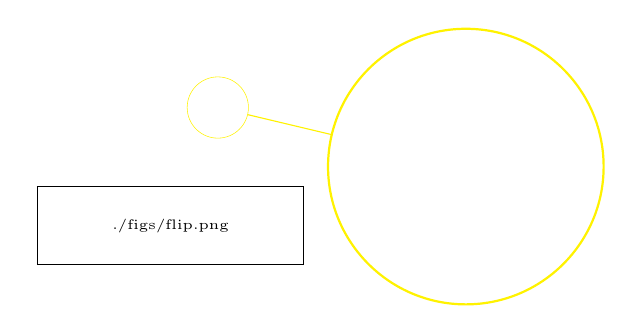
\begin{tikzpicture}[spy using outlines={circle,yellow,magnification=4.5,size=3.5cm, connect spies}]
        \node {\pgfimage[width=0.28\textwidth]{./figs/flip.png}};
        \spy on (.6,1.5) in node [left] at (5.5,0.75);
      \end{tikzpicture}
    }
    &
    \resizebox{0.45\columnwidth}{!}
    {
      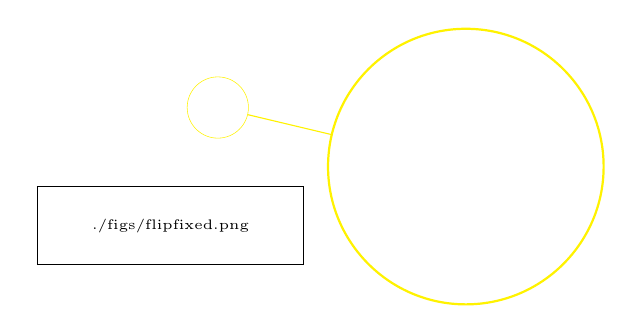
\begin{tikzpicture}[spy using outlines={circle,yellow,magnification=4.5,size=3.5cm, connect spies}]
        \node {\pgfimage[width=0.28\textwidth]{./figs/flipfixed.png}};
        \spy on (0.6,1.5) in node [left] at (5.5,0.75);
      \end{tikzpicture}
    }
    \vspace{-0.1cm}
  \end{tabular}
%\includegraphics[width=100pt]{flip.png}\includegraphics[width=100pt]{flipfixed.png}
\caption{\emph{Left}: Output generated by a network trained with inverse consistency, evaluated on a grid (not randomly); the loss cannot detect that these maps flip the pair of pixels in the upper right corner, as that error is not represented in the composed map. \emph{Right}: Output from a network trained with random evaluation off of lattice points.} \label{fig:flips}
\end{figure}

% \begin{figure}
%   \centering
%   \begin{tabular}{cc}
%     {\footnotesize (a) Forward map}  & \footnotesize{(b) Backward map} \\
%     \resizebox{0.43\columnwidth}{!}
%     {
%       \input{./xfig_figs/off_grid_sample_illustration_forward_map.tikz}
%     }
%     &
%     \resizebox{0.43\columnwidth}{!}
%     {
%       \input{./xfig_figs/off_grid_sample_illustration_backward_map.tikz}
%     }
%     \\
%     \footnotesize{(c) Forward displacement}  & \footnotesize{(d) Backward displacement} \\
%     \resizebox{0.43\columnwidth}{!}
%     {
%       \input{./xfig_figs/off_grid_sample_illustration_forward_map_function.tikz}
%     }
%     &
%     \resizebox{0.43\columnwidth}{!}
%     {
%       \input{./xfig_figs/off_grid_sample_illustration_backward_map_function.tikz}
%     }
%   \end{tabular}
%   \vspace{-0.2cm}
%   \caption{In this example, grid points (solid black circles) map to each other inverse consistently. The forward map (a) is inverted by the backward map (b). However, folding of the space occurs as the middle two points swap positions. Off-grid points map under linear interpolation according to (c/d). We see that the interpolated displacements for the small solid blue circle do not result in an invertible map. Hence, this mismatch would be penalized by the inverse consistency loss, but only when evaluated off-grid.}
%   \label{fig:off_grid_resampling}
% \end{figure}

%\vskip0.5ex

\begin{figure}
  \centering
  \includegraphics[width=0.9\columnwidth]{fwd_bwd_displacement.pdf}
  \caption{\label{fig:off_grid_resampling}In this example, grid points (\textcolor{black}{$\bullet$}) map to each other inverse consistently. The forward map (a) is inverted by the backward map (b) and folding of the space occurs as the middle two points swap positions. Off-grid points map under linear interpolation according to (c/d). The interpolated displacements for (\textcolor{red}{$\bullet$}) do not result in an invertible map. Hence, this mismatch would be penalized by the inverse consistency loss, but only when evaluated off-grid.}
  \vspace{-0.2cm}
\end{figure}


\noindent
\textbf{Random evaluation of inverse consistency loss}.
$\mathcal{L}_{\text{inv}}^{AB}$ can be evaluated by approximating the $L^2$ norm, assuming constant values over the grid cells. In many cases, this is sufficient. However, as Fig.~\ref{fig:flips} illustrates, swapped locations may occur in uniform regions  where a registration network only sees uniform background. This swap, composed with itself, is the identity as long as it is only evaluated at the center of pixels/voxels. Hence, the map appears invertible to the loss. However, outside the centers of pixels/voxels, the map is not inverse consistent when combined with linear interpolation. To avoid such pathological cases, we approximate the $L^2$ norm by random sampling. This forces interpolation and therefore results in non-zero loss values for swaps. Fig.~\ref{fig:off_grid_resampling} shows why off-grid sampling combined with inverse consistency is a stronger condition than only considering deformations at grid points. In practice, we evaluate the loss



%\begin{align}
%  %\begin{split}
%    & \mathcal{L}_{\text{inv}}(\Phi_\theta^{AB},\Phi_\theta^{BA}) = \left\| (D_\theta^{AB}) \circ \Phi_\theta^{BA}  + D_\theta^{BA} \right\|_2^2\\
%    & ~~= \mathbb{E}_{x \sim \mathcal{U}(0,1)^N} \left[(D_\theta^{AB}) \circ \Phi_\theta^{BA}  + D_\theta^{BA}\right]^2(x) \nonumber \\
%    & ~~\approx \nicefrac{1}{N_p}\sum\nolimits_{i} \left([(D_\theta^{AB}) \circ (D_\theta^{BA} + \operatorname{Id})  + D_\theta^{BA}] (x_i + \epsilon_i) \right)^2  \nonumber \\
%    & ~~= \nicefrac{1}{N_p}\sum\nolimits_{i} \left([D_\theta^{AB} \circ (D_\theta^{BA} \circ (x_i + \epsilon_i) + x_i + \epsilon_i) \right.  \nonumber \\
%    & ~~~~~~~~~~~~~~~~~~~~~~~~+ \left. D_\theta^{BA} \circ (x_i + \epsilon_i)]\right)^2 \nonumber
%  %\end{split}
%\end{align}
\vspace{-0.1cm}
{\centering
\scalebox{0.87}{\parbox{1.15\linewidth}{%
\begin{align}
  %\begin{split}
    & \mathcal{L}_{\text{inv}}(\Phi_\theta^{AB},\Phi_\theta^{BA}) = \left\| (D_\theta^{AB}) \circ \Phi_\theta^{BA}  + D_\theta^{BA} \right\|_2^2 \nonumber \\
    & ~~= \mathbb{E}_{x \sim \mathcal{U}(0,1)^N} \left[(D_\theta^{AB}) \circ \Phi_\theta^{BA}  + D_\theta^{BA}\right]^2(x)  \nonumber \\
    & ~~\approx \nicefrac{1}{N_p}\sum\nolimits_{i} \left([(D_\theta^{AB}) \circ (D_\theta^{BA} + \operatorname{Id})  + D_\theta^{BA}] (x_i + \epsilon_i) \right)^2  \\
    & ~~= \nicefrac{1}{N_p}\sum\nolimits_{i} \left([D_\theta^{AB} \circ (D_\theta^{BA} \circ (x_i + \epsilon_i) + x_i + \epsilon_i) \right.  \nonumber \\
    & ~~~~~~~~~~~~~~~~~~~~~~~~+ \left. D_\theta^{BA} \circ (x_i + \epsilon_i)]\right)^2\enspace, \nonumber
  %\end{split}
\end{align}
}}}





% \begin{multline}
%   \mathcal{L}_{inv}(\Phi_\theta^{AB},\Phi_\theta^{BA}) = ||(D_\theta^{AB}) \circ \Phi_\theta^{BA}  + D_\theta^{BA} ||_2^2 \\
%   = \mathbb{E}_{x \sim \mathcal{U}(0,1)^N} \left[(D_\theta^{AB}) \circ \Phi_\theta^{BA}  + D_\theta^{BA}\right]^2(x)\\
%   \approx \frac{1}{N_p}\sum_{i=1}^{N_p} \left([(D_\theta^{AB}) \circ (D_\theta^{BA} + \operatorname{Id})  + D_\theta^{BA}] (x_i + \epsilon_i) \right)^2 \\
%     = \frac{1}{N_p}\sum_{i=1}^{N_p} ([D_\theta^{AB} \circ (D_\theta^{BA} \circ (x_i + \epsilon_i) + x_i + \epsilon_i) \\ + D_\theta^{BA} \circ (x_i + \epsilon_i)])^2, 
% \end{multline}

where $N_p$ is the number of pixels/voxels, $\mathcal{U}(0,1)^N$ denotes the uniform distribution over $[0,1]^N$, $x_i$ denotes the grid center coordinates and $\epsilon_i$ is a random sample drawn from a multivariate Gaussian with standard deviation set to the size of a pixel/voxel in the respective spatial directions. 

%To implement this model we 1) sample random image pairs to evaluate the expectations, 2) reformulate the inverse consistency term with respect to the predicted displacement fields, and 3) propose a random sampling strategy for the inverse consistency loss to avoid foldings.




%\begin{equation}
%    \mathcal{L}_{inv}^{A,B} = ||(D_{AB}) \circ (D_{BA} + id)  + D_{BA} ||_2^2
%\end{equation}
%\begin{equation}
%    = \mathbb{E}_{x \sim [0, 1]^N} \left[(D_{AB}) \circ (D_{BA} + id)  + D_{BA}\right]^2(x)
%\end{equation}
%\begin{equation}
%    \approx \frac{1}{\text{num pixels}}\sum \left([(D_{AB}) \circ (D_{BA} + id^{func})  + D_{BA}] (id^{grid} + \epsilon) \right)^2
%\end{equation}
%\begin{equation}
%    = \frac{1}{\text{num pixels}}\sum \left([D_{AB} \circ (D_{BA} \circ (id^{grid} + \epsilon) + id^{grid} + \epsilon) + D_{BA} \circ (id^{grid} + \epsilon)]\right)^2
%\end{equation}

%where $\epsilon$ be some noise with standard deviation on the order of pixel stride and shape (batchsize x 3 x height x width x depth),

%When computing $\mathcal{L}_{inv}^{A,B}$ one is tempted to approximate the $L^2$ norm assuming the values are constant over the grid cells. This does usually work, so unlike the boundaries section you don't necessarily need to implement this section. However, for some network architectures the neural network can learn a local minimum where it picks a set of pixels to always swap with each other. This swap, composed with itself, is the identity as long as its only evaluated at the center of pixels. Therefore the loss thinks that the transform is invertible. However outside the centers of pixels this type of transform is not invertible. This is of course a problem, but suggests a solution:  actually compute the $L^2$ norm over our function in the region of interest by sampling its output at a grid with noise added. Letting $\epsilon$ be some noise with standard deviation on the order of pixel stride and shape (batchsize x 3 x height x width x depth), 

%This expression is visually unpleasant, but numerically effective.

\section{Experiments}
\label{section:experiments}

Our experiments address several aspects:  First, we compare our approach to \emph{directly} optimizing the maps $\Phi^{AB}$ and $\Phi^{BA}$ on a 2D toy dataset of $128 \times 128$ images. Second, on a 2D toy dataset of $28 \times 28$ images, we assess the impact of architectural and hyperparameter choices. Finally, we assess registration performance on real 3D MR images of the knee. 

\subsection{Datasets}
\label{subsection:datasets}

\noindent
\textbf{MNIST}. We use the standard MNIST dataset with images of size $28 \times 28$, restricted to the number ``5'' to make sure we have semantically matching images. For training/testing, we rely on the standard partitioning of the dataset.

%\todo{How many for training and testing?}

\vskip0.5ex
\noindent
\textbf{Triangles \& Circles.} We created 2D triangles and circles ($128 \times 128$) with radii and centers varying uniformly in $[.2,.4]$ and $[.4,.7]$, respectively. 
Pixels are set to 1 inside a shape and smoothly decay to -1 on the outside. We train using 6,000 images and test on 6,000 separate images\footnote{Code to generate images and replicate these experiments is available at \url{https://github.com/uncbiag/ICON}}.

% \emph{MNIST}: Our initial discovery of this effect (regularization only through inverse consistency) was made while playing around with MNIST digits. We restrict our analysis to the images labeled "5" to help make sure each pair of images has a semantically correct correspondence. We use the standard train/test split of MNIST. 
% \\
% \emph{Triangles and Circles}:\todo{re-run experiments at uniform 64x64}
% We use also use a synthetic dataset composed of a mix of triangles and circles. The centers and radii of the trianges and circles vary uniformly, with radius ranging from .2 to .4 and the center coordinate ranging from .4 to .7. The angle of the triangles is selected randomly. This dataset takes two forms with different difficulties: The 'filled' triangles and circles dataset attains a value of 1 inside the shape and smoothly ramps to -1 outside the shape, while the hollow version of this dataset is zero everywhere except near the boundary: specifically, it is one minus the square, pixelwise, of the filled dataset. In each case, there is a training set of 6000 images, and a test set of 6000 images. Code to generate this dataset is included with this papser.\\ 

\vskip0.5ex
\noindent
\textbf{OAI knee dataset}. These are 3D MR images from the Osteoarthritis Initiative (OAI). Images are downsampled to size $192 \times 192 \times 80$,
%\todo{Don't you upsample for evaluation?} 
normalized such that the 1th percentile is set to 0, the 99th percentile is to 1, and all values are clamped to be in $[0,1]$. As a preprocessing step, images of left knees are mirrored along the left-right axis. The dataset contains ~\mn{2,532} training images and 301 test pairs. 

\subsection{Architectures}
\label{subsection:architectures}

We experiment with four neural network architectures. All networks output displacement fields, $D_\theta^{AB}$. We briefly outline the differences below, but refer to the suppl. material for details. The first network is an \textbf{MLP} with 2 hidden layers and ReLU activations. The output layer is reshaped into size $2 \times W \times H$. %and to represent the grid of displacement vectors $\Phi$ is computed.
Second, we use a convolutional encoder-decoder network (\textbf{Enc-Dec}) with 5 layers each, reminiscent of a U-Net \emph{without} skip connections. 
Our third network uses 6 convolutional layers without up- or down-sampling. The input to each layer is the concatenation of the outputs of all previous layers (\textbf{ConvOnly}). 
Finally, we use a \textbf{U-Net} with skip and residual connections. The latter is similar to \textbf{Enc-Dec}, but uses LeakyReLU activations and batch normalization.
%\todo{Is there a particular reason why some networks appear to use Relu, others LeakyRelu, some batchnorm and others not. It seems to muddy the waters a bit.} 
%The latter three networks output two feature maps at the final layer, interpreted as a grid of displacement vectors.
In all architectures, the final layer weights are initialized to 0, so that optimization starts at a network outputting a zero displacement field.



% In this paper we refer to four neural network architectures: Dense, Encoder-Decoder, U-Net, and Convolutions. Here are the details of each.\\
% Dense: Dense refers to a Multilayer perceptron with no special structure. We use hidden layers of size 8000 and 3000, and a relu nonlinearity. The output layer is dimension 2 x W x H, which is reshaped into a grid of displacement vectors from which $\Phi$ is calculated as above.\\
% Encoder-Decoder: The Encoder-Decoder used in this paper is composed of a convolutional encoder and decoder, resembling a U-Net with no skip connections. Each layer consists of a stride 2 convolution or transpose convolution with kernel size 3x3 in the encoder and 4x4 in the decoder, followed by a ReLu nonlinearity. The layers have 16, 32, 64, 256, and 512 features in the encoder, and 256, 128, 64, 32, and 16  features in the decoder.\\
% Convolutions: This refers to a simple architecture consisting of six convolution layers, each with 5x5 kernel, ReLu nonlinearity,  and 10 output features. No downsampling or upsampling is performed. Each layer is fed as input the concatenation of the outputs of all previous layers. \\ 
% U-Net: We use a U-Net with skip and residual connections. The convolutional layers have the same shapes and output dimensions as the encoder decoder network, but use Leaky Relu activation placed before convolution instead of after. In addition, batch normalization is inserted before each convolution, and a residual connection is routed around each convolution, using upsampling or downsampling as required to match the image size. 
% In each case, the weights of the final layer of the neural network are initialized to zero instead of randomly, such that training begins with the network outputting a displacement field of zero.

% \todo[inline]{I think it would be good to have a separate dataset section describing the datasets, sample sizes, etc.  Also to more clearly describe how these datasets were generated, in particular, for the circles and triangles examples.}

% \todo[inline]{Seems a bit random still here in the explanation when what dataset is used. Sometimes it is solid and sometimes not. But it is not really clear why.}


\subsection{Regularization by approx. inverse consistency}
\label{subsec:imperfect_inverse_consistency}

\begin{figure}
   \resizebox{\columnwidth}{!}{
     \centering
     \includegraphics[width=1.0\columnwidth]{noise_effect_tex.pdf}
     %\includegraphics[width=1.0\columnwidth,angle=-90]%{noise_effect.png}
   }
   \caption{Comparison between \textbf{U-Net} results and \textbf{direct optimization} (no neural network; over $\Phi_\theta^{AB}$ and $\Phi_\theta^{BA}$) w/ and w/o added noise,  using the inverse consistency loss with $\lambda = 2,048$. Direct optimization w/o noise leads to irregular maps, while adding noise or using the \textbf{U-Net} improves map regularity (best viewed zoomed).} \label{fig:regularity_by_inexact_inverse_consistency}
     %{While both methods are able to drive the composition of deformations to the identity, in the neural network case this forces smoothness, while in the direct optimization case this does not force smoothness, merely invertability. Result of directly optimizing the displacement maps $D^{AB}$ and $D^{BA}$ to minimize our loss, with and without noise added during the computation of $\Phi$ from $D$. When noise is added to the maps, regularized transforms are produced, while without noise no regularization occurs. No neural network is involved in this experiment.} 
     \vspace{-0.2cm}
\end{figure}

Sec.~\ref{subsec:h1_by_approximate_inverse_consistency} formalized that approximate inverse consistency results in regularizing effects. Specifically, when $\Phi_\theta^{AB}$ is approximately the inverse of $\Phi_\theta^{BA}$, the inverse consistency loss $\mathcal{L}^{AB}_{\text{inv}}$ can be approximated based on Eq.~\eqref{EqH1regularization}, highlighting its implicit $H^1$ regularization.
%as $\varepsilon^2 \| \nabla \psi \sqrt{\operatorname{Jac}(\psi)} \|^2$.\todo{FX: This notation needs to be fixed once you have finalized your notation.}
We investigate this behavior by three experiments: 
\mn{Pair-wise image registration (1) with artificially added noise (\textbf{noise}) and (2) without (\textbf{no noise}) artificially added noise, and (3) population-based registration via a \textbf{U-Net}.}
% (1) Pair-wise image registration without noise (\textbf{no noise}); (2) Pair-wise image registration with artificially added noise (\textbf{noise}); and (3) Population-based . 
Fig.~\ref{fig:regularity_by_inexact_inverse_consistency} shows some sample results, supporting our theoretical exposition of Sec.~\ref{subsec:h1_by_approximate_inverse_consistency}: Pair-wise image registration without noise results in highly irregular transformations even though the inverse consistency loss is used. Adding a  small amount of Gaussian noise with standard deviation of 1/8th of a pixel (similar to the inverse consistency loss magnitudes we observe for a deep network) to the displacement fields before computing the inverse consistency loss, results in significantly more regular maps. Lastly, using a \textbf{U-Net} yields highly regular maps. Notably, all three approaches result in approximately inverse consistent maps. The behavior for pair-wise image registration elucidates why inverse consistency has not appeared in the classical (pair-wise) registration literature as a replacement for more complex spatial regularization. The proposed technique \emph{only} results in regularity when inverse consistency errors are present.

\vskip0.5ex
\emph{In summary, our theory is supported by our experimental results: approximate inverse consistency regularizes maps.}

%In the above experiment, when the map was parameterized directly, the optimizer was able to drive $e(x)$ to zero on the majority of the images. Hence, the gradient of $\Phi$ was not restricted. On the other hand, when the map was parameterized using a neural network, the gradient of $\Phi$ was penalized as $e$ did not go to zero. In light of this result, we hypothesize that if we artificially introduce an error term $e(x)$ to the direct parameterization of the transform, then optimization will also yield smooth transforms. To test this, we move to a dataset of intermediate difficulty, filled in triangles and circles at a resolution of 128 x 128. We parameterize the transforms as two 128 x 128 x 2 displacement maps, each voxel of which is treated as a parameter for optimization. At each step we add these displacement maps to the identity map as well as to some Gaussian noise with magnitude 1/8th of a pixel (roughly the magnitude of $e(x)$ found in our successful neural network experiments) to obtain $\Phi^{AB}$ and $\Phi^{BA}$. We then optimize $\mathcal{L}(\Phi^{AB}, \Phi^{BA})$ as above. As a control, we also perform this experiment with noise magnitude zero, i.e., without any noise. Fig.~\ref{fig:regularizing_via_noise} illustrates that as expected, introducing noise serves to regularize the transforms, providing evidence that our understanding of the weak regularization imposed by our loss is correct. 

%\begin{figure}

\subsection{Regularization for different networks}

\begin{table}
\centering
\resizebox{\columnwidth}{!}{%
\begin{tabular}{lllllllll}
\toprule
& \multicolumn{8}{c}{\textbf{MNIST}}  \\ 
\midrule
Network $\rightarrow$ & \multicolumn{2}{c}{\bf MLP} & \multicolumn{2}{c}{\bf Enc-Dec} &\multicolumn{2}{c}{\bf U-Net} & \multicolumn{2}{c}{\bf ConvOnly} \\
\midrule
$\lambda$ $\downarrow$ & Dice & Folds~~ & Dice & Folds &  Dice & Folds & Dice & Folds  \\
\midrule
64 & 0.92 & 26.61 & 0.80 & 0.15 & \textbf{0.93} & 3.87 & \textbf{0.93} & 30.20  \\
128 & \textbf{0.92} & 9.95 & 0.77 & 0.08 & \textbf{0.92} & 1.45 & 0.90 & 16.27 \\
256 & \textbf{0.91} & 2.48 & 0.72 & 0.01 & 0.90 & 0.41 & 0.88 & 7.17  \\
512 & \textbf{0.90} & 0.72 & 0.66 & 0.03 & 0.89 & 0.09 & 0.85 & 3.12  \\
1,024 & \textbf{0.88} & 0.34 & 0.62 & 0.06 & 0.86 & 0.02 & 0.81 & 0.54\\
2,048 & \textbf{0.87} & 0.16 & 0.63 & 0.00 & 0.73 & 0.09 & 0.76 & 0.07\\
\bottomrule
\end{tabular}
}\\
\resizebox{\columnwidth}{!}{%
\begin{tabular}{lllllllll}
\toprule
& \multicolumn{8}{c}{\textbf{Triangles \& Circles}} \\ 
\midrule
Network $\rightarrow$ & \multicolumn{2}{c}{\bf MLP } & \multicolumn{2}{c}{\bf  Enc-Dec} &\multicolumn{2}{c}{\bf U-Net} & \multicolumn{2}{c}{\bf ConvOnly} \\
\midrule
$\lambda$ $\downarrow$  & Dice & Folds~~ & Dice & Folds &  Dice & Folds & Dice & Folds  \\
\midrule
64 & \textbf{0.98} & 1.24 & 0.94 & 3.50 & \textbf{0.98} & 2.74 & 0.97 & 12.57  \\
128 & \textbf{0.98} & 0.73 & 0.90 & 2.71 & \textbf{0.98} & 1.59 & 0.96 & 10.15  \\
256 & \textbf{0.98} & 0.27 & 0.88 & 1.11 & 0.97 & 1.14 & 0.96 & 8.49  \\
512 & \textbf{0.97} & 0.10 & 0.87 & 0.65 & 0.96 & 0.70 & 0.94 & 6.61  \\
1,024 & \textbf{0.96} & 0.03 & 0.86 & 0.22 & 0.95 & 0.25 & 0.92 & 3.91  \\
2,048 & \textbf{0.95} & 0.03 & 0.85 & 0.15 & 0.94 & 0.09 & 0.89 & 2.18  \\
\bottomrule
\end{tabular}
}
\caption{Network performance across architectures and regularization strength $\lambda$. \textbf{MLP} / \textbf{U-Net} perform best. All methods work.}\label{tab:registration_across_architectures}
\vspace{-0.2cm}
\end{table}


\begin{figure}
  \includegraphics[width=0.97\columnwidth]{TrianglesFivesCombined-compressed.pdf}
  % \resizebox{\columnwidth}{!}{
  % \begin{tabular}{c}
  %   \includegraphics[width=1.0\columnwidth]{Foobar} \\
  %   \includegraphics[width=1.0\columnwidth,angle=-90]{Triangles-2}
  % \end{tabular}
  % }
%\includegraphics[width=160pt]{tri_quant.png}
%\includegraphics[width=160pt]{mnist_quant.png}

\caption{Comparison of networks as a function of $\lambda$. \textbf{U-Net} and \textbf{MLP} show the best performance due to their ability to capture long and short range dependencies. \textbf{Enc-Dec} and \textbf{ConvOnly}, which capture only long range and only short range dependencies, resp., also learn regular maps, but for a narrower range of $\lambda$. In all cases, maps become smooth for sufficiently large $\lambda$. Best viewed zoomed.} \label{fig:registration_across_architectures}
\vspace{-0.2cm}
\end{figure}

Sec.~\ref{subsec:imperfect_inverse_consistency} illustrated that approximate inverse consistency yields regularization effects which translate to regularity for network predictions, as networks will, in general, not achieve perfect inverse consistency. A natural next question to ask is ``how much the results depend on a particular architecture''? To this end, we assess four different network types, focusing on MNIST and the triangles \& circles data. We report two measures on held-out images: the \emph{Dice score} of pixels with intensity greater than $0.5$, and the mean number of \emph{folds}, \ie, pixels where the volume form $\mathrm{d}V$ of $\Phi$ is negative.

%The first question we address is whether the regularity of the transforms produced by our technique is enforced by the inverse consistency loss, or if the observed regularity is, in fact, an artifact of the network design.  
%If an experimenter combines our loss with their architecture, are they likely to obtain good results for an appropriate $\lambda$? 
%To that end, we use the same loss with four neural network architectures and two different toy datasets: all the numbers "5" from \texttt{MNIST}, and a collection of 6,000 triangles and circles. 

% \todo[inline]{I think it would also be good to somewhere at the beginning describe the different network architectures you used. Some of this material should likely go into supplementary material. Also, do you mean fully connected when you say dense?}

\vskip0.5ex
One hypothesis as to how network design could drive smoothness %-- which could invalidate our claim that transform regularity is driven by the loss --
would be that smoothness is induced by convolutional layers (which can implement a smoothing kernel). 
If this were the case, we would expect the \textbf{MLP} to produce irregular maps with a high number of folds. Vice versa, since the \textbf{MLP} has no spatial prior, obtaining smooth transforms would indicate that smoothness is promoted by the loss itself. The latter is supported by Fig.~\ref{fig:registration_across_architectures}, showing regular maps even for the \textbf{MLP} when $\lambda$ is sufficiently large. Note that $\lambda=0$ in Fig.~\ref{fig:registration_across_architectures} corresponds to an unregularized MSE solution, as discussed in Sec.~\ref{subsection:regularization_thoughts_and_sorting}; maps are, as expected, highly irregular and regularization via inverse consistency is clearly needed.

% see Fig.~\ref{fig:registration_across_architectures}), indicating that the transform is regularized by the loss function as opposed to any spatial prior in the network.  
%if we obtain smooth transforms from a dense network then we know that the smoothness is coming from the loss
% the regularity we observe in the transform is driven by the loss function, would be that the smoothness we see in U-Net results actually comes from the convolution operator in our neural network, which can implement a smoothing kernel. If this were the case, we would expect a dense neural network trained on our loss to produce transforms with a high number of folds, or some other sort of qualitative deficiency. Alternatively, since a dense network has no spatial prior, if we see smooth transforms from a dense network then we know that the smoothness is coming from the loss. To test this, we train a dense (fully connected) neural network on our 2-D datasets. We obtain smooth results (see Fig.~\ref{fig:registration_across_architectures}), indicating that the transform is regularized by the loss function as opposed to any spatial prior in the network.  

\vskip0.5ex
A second hypothesis is that regularity results from a \emph{bottleneck} structure within a network, \eg, a \textbf{U-Net}. In fact, Bhalodia \etal~\cite{bhalodia19} show that autoencoders tend to yield smooth maps. To assess this hypothesis, we focus on the \textbf{Enc-Dec} and \textbf{ConvOnly} type networks; the former has a bottleneck structure, while the latter does not.
Fig.~\ref{fig:registration_across_architectures} shows some support for the hypothesis that a bottleneck promotes smooth maps: for a specific $\lambda$, \textbf{Enc-Dec} appears to have more strongly regularized outputs compared to \textbf{U-Net}, with \textbf{ConvOnly} being the most irregular.
%the Encoder-Decoder appears to have intensely regularized outputs %compared to the U-Net, while the pure convolution (with no upsampling %or downsampling) network has more irregular outputs than the U-Net. 
Yet, higher values of $\lambda$ (\eg, 1,024 or 2,048) for \textbf{ConvOnly} yield equally smooth maps. Overall, a bottleneck structure does have a regularizing effect, but regularity can also be achieved by appropriately weighing the inverse consistency loss (see Tab.~\ref{tab:registration_across_architectures}).

\vskip0.5ex
\emph{In summary, our experiments indicate that the regularizing effect of inverse consistency is a robust property of the loss, and should generalize well across architectures.}

% As a result, the ideal value of $\lambda$ appears to vary with network architecture, in these extreme cases all the way from 64 for the autoencoder to 2048 or 1024 for the purely convolutional network. However, for appropriate values of $\lambda$ all three networks work.
% \todo[inline]{Wasn't the argument that one can use a wide range of $\lambda$'s and hence these networks are easy to tune. This seems to be contradicted by what you say above.}

% To test this we create two networks, one by removing the downsampling and upsampling layers of the U-Net, leaving a network composed only of full resolution convolutions, and another where we strip out the skip connections, leaving an Encoder-Decoder. Fig.~\ref{fig:registration_across_architectures} shows some support for the hypothesis that a bottleneck has a smoothing effect: the Encoder-Decoder appears to have intensely regularized outputs compared to the U-Net, while the pure convolution (with no upsampling or downsampling) network has more irregular outputs than the U-Net. As a result, the ideal value of $\lambda$ appears to vary with network architecture, in these extreme cases all the way from 64 for the autoencoder to 2048 or 1024 for the purely convolutional network. However, for appropriate values of $\lambda$ all three networks work.
% \todo[inline]{Wasn't the argument that one can use a wide range of $\lambda$'s and hence these networks are easy to tune. This seems to be contradicted by what you say above.}

%The third hypothesis we investigated is that the smoothness comes from the texture of the data, because a unique smooth map aligns each bump and crag in the optimal way~\cite{niethammer2019metric}. The second dataset of filled shapes was included to check whether this was the case, with large textureless regions inside the shapes. Fig.~\ref{fig:registration_across_architectures} illustrates that in these textureless regions inverse consistency is still sufficient to force a neural network to output a smooth transform. 

%\subsection{ Comparison to direct optimization of $\Phi_{AB}$ / $\Phi_{BA}$}
%% \todo[inline]{The following sentence is a bit complex and should be simplified. Need to read the paper to do this. Or Hastings can you do it, as you read this paper in more detail?}
%%Bhalodia et al.~\cite{bhalodia19} found that registration neural networks operating on a population of images, when forced to match the output of another neural network while passing the registration information through a bottleneck layer, necessarily output transforms on a submanifold of the space of all transforms. Further, they found that transforms in that submanifold are smooth. If this effect is driving the smoothness of our results, we expect that our loss should not produce smooth results when the transforms themselves are optimized instead of network weights.
%In this experiment, we compare our approach to directly optimizing vectors of the \emph{deformation field}, as typically done in traditional pairwise image registration. We specifically focus on the synthetic triangles \& circles dataset and train a \textbf{U-Net} architecture with the inverse consistency loss and $\lambda=2048$. 
%%We investigate aligning triangles and circles, but this time as outlines instead of filled in and at a resolution of 128 x 128 instead of 28 x 28. We train a U-Net architecture with $\lambda = 2048$ on this dataset and loss. We compare it to optimizing vectors of the deformation field directly, as in traditional pairwise image registration. 
%As can be seen from Fig.~\ref{fig:high_res_shape_outlines} (columns 4 \& 7), both approaches produce invertible transforms, since, in each case, the composition of $\Phi^{AB}$ and $\Phi^{BA}$ is close to the identity.
%%Both 
%% to produce invertible transforms, as can be seen in columns 4 and 7 of Fig.~\ref{fig:high_res_shape_outlines}, since in each case the composition of $\Phi_{AB}$ and $\Phi_{BA}$ is close to the identity. 
%  However, training the network with the proposed inverse consistency loss yields smooth deformations, while direct optimization of the deformation field produces very ragged deformations. While invertible, such deformations are not semantically meaningful. This provides strong empirical evidence that the inverse consistency loss exerts implicit regularization applied to the gradient, resulting from the neural network's uncertainty about how it will behave with swapped inputs 
%  (especially in textureless areas). When this uncertainty is removed by always using the same pair of images, the implicit gradient penalty vanishes.
%This also elucidates why inverse consistency has not appeared in the classical image registration literature as a replacement for more complicated smoothness constraints. The proposed technique only solves the aperture problem in the presence of a population, and so is not suitable for direct optimization.

%% \todo[inline]{Agree! The population aspect is, to me, the key factor for smoothness ... as the data acts as an implicit regularizer. Also, it might be due to SGD, e.g., as it is hypothesized that SGD prefers ``simple'' solutions, see, e.g., 
%  https://arxiv.org/pdf/1909.12051.pdf}


%    \centering
%    \begin{tabular}{c c c c}
%       Image A & With Noise & Without Noise & Image B \\
%    \end{tabular}
%    \includegraphics[width=1\columnwidth]{noise_small.png}
%    \caption{Result of directly optimizing the displacement maps $D^{AB}$ and $D^{BA}$ to minimize our loss, with and without noise added during the computation of $Phi$ from $D$. When noise is added to the maps, regularized transforms are produced, while without noise no regularization occurs. No neural network is involved in this experiment.}
%    \label{fig:regularizing_via_noise}
%\end{figure}

\subsection{Performance for 3D image registration}

% \todo[inline]{Here you also give some details on batchsize etc., but you don't do this for any of the other experiments. Would be good to have a section to summarize all of these different network settings for all the experiments. Could also go partially into the supplementary material.}

For experiments on real data, we focus on the 3D OAI dataset. To demonstrate the versatility of the advocated inverse consistency loss in promoting map regularity, we refrain from affine pre-registration (as typically done in earlier works) and simply compose \mn{the maps of} \emph{multiple U-Nets} instead. In particular, we compose up to four U-Nets \mn{as follows:} A composition of two U-Nets is initially trained on low-resolution image pairs. Weights are then frozen and this network is composed with a third U-Net, trained on high-resolution image pairs. This network is then optionally frozen and composed with a fourth U-Net, again trained on high-resolution image pairs. During this multi-step training, the weighting of the inverse consistency loss is gradually increased. We train using ADAM \cite{Kingma15a} with a batch size of 128 in the low-res. stage, and a batch size of 16 in the high-res. stage. MSE is used as image similarity measure.

\vskip0.5ex
We compare our approach, \textcolor{ggreen}{InverseConsistentNet (\texttt{ICON})}, against the methods of \cite{shen2019networks}, in terms of (1) cartilage Dice scores between registered image pairs~\cite{AmbellanTackEhlkeetal.2018} (based on manual segmentations) and (2) the number of folds. The segmentations are not used during training and allow quantifying if the network yields semantically meaningful registrations. Tab.~\ref{tab:oai_results} lists the corresponding results, Fig.~\ref{fig:teaser} shows several example registrations. Unlike the other methods in Tab.~\ref{tab:oai_results}, except where explicitly noted, \mn{\texttt{ICON} does not require affine pre-registration. Since affine maps are inverse consistent, they are not penalized by our method.}
%, as the deformation can capture the affine component,
Notably, despite its simplicity, \texttt{ICON} yields performance (in terms of Dice score \& folds) comparable to more complex, explicitly regularized methods. We emphasize that our objective is not to outperform existing techniques, but to present evidence that regular maps can be learned \emph{without} carefully tuned regularizers.


% Tab.~\ref{tab:registration_across_architectures} indicated good performance across architectures (for appropriate $\lambda$'s), but in particular for the \textbf{MLP}. 
% An \textbf{MLP} is, of course, not possible in 3D. 
% Hence, we train a 3D \textbf{U-Net} instead. 
% To compete with other state-of-the-art registration techniques (\cf \cite{shen2019networks}), we rely on a more expressive architecture, composed of multiple U-Net steps and a training schedule for $\lambda$ (see supp. mat. for details). We train using SGD with a batch-size of 128 during low-resolution pre-training and a batch-size of 8 during training with high-resolution images.

% We use SSD image similarity, and use a batch size of 128 during low resolution pretraining, and a batch size of 8 during the final high resolution training. We use a training schedule for lambda, ending on 3200, as described in more detail in the supplementary material. Training takes approximately 4 days on 4 RTX 2080s. We compare cartilage Dice scores between registered image pairs~\cite{AmbellanTackEhlkeetal.2018} based on manual segmentations. These segmentations are not used during training and allow quantifying if the network yields semantically meaningful registrations. Tab.~\ref{tab:oai_results} shows the good performance of our approach. Notably, unlike the other methods in the table except where explicitly noted, our technique has no affine pre-registration, as the deformation can capture the affine component since affine maps are inverse consistent, and hence not penalized by our method.

% During this process we determined one unfortunate property of our loss function, which is that it demands a large batch size to capture large deformations, as with a batch size less than 128 the network did not capture the full range of shifts and warps present in the OAI dataset. For this reason, we  heavily downsampled the input in order to fit batches into VRAM: the original OAI images are 384 x 384 x 160, and the registration methods we compared to were all able to run at 192 x 192 x 80, while our network accepted images 96 x 96 x 40. For this reason, we upsample the transforms produced by our network to 192 x 192 x 80 so that our results can be directly compared with these other methods. 

\vskip0.5ex
\emph{In summary, using \texttt{ICON} yields (1) competitive Dice scores, (2) acceptable folds and (3) fast performance.}\\[-0.6cm]

%reduced computation time (as testing just boils down to a forward pass through the model). 

% \begin{figure}
%   \centering
%   \includegraphics[width=0.32\columnwidth]{oai-a-trimmed.png}\hfill
%   \includegraphics[width=0.32\columnwidth]{oai-warped-b-trimmed.png}\hfill
%   \includegraphics[width=0.32\columnwidth]{oai-b-trimmed.png}
%   % \resizebox{\columnwidth}{!}{
%   % \begin{tabular}{ccc}
%   %   \includegraphics[width=0.335\columnwidth]{oai-a-trimmed.png} &
%   %   \includegraphics[width=0.335\columnwidth]{oai-warped-b-trimmed.png} &
%   %   \includegraphics[width=0.335\columnwidth]{oai-b-trimmed.png}
%   % \end{tabular}
%   % }
%   \caption{Example OAI registration result generated by our network. \emph{Left to right}: fixed, warped moving, and moving image. The warped moving image is visually very similar to the fixed image; the transformation grid (colored) is, as desired, smooth.}
%   %OAI data is challenging for a registration technique because of the large variation in size and shape of the joint and the framing of the MR images.}
%     \label{fig:oai_example}
% \end{figure}


\begin{table}
\begin{small}
\centering
\resizebox{\columnwidth}{!}{%
\begin{tabular}{lllll}
\toprule
\textbf{Method} &  $\mathcal{L}_{\text{sim}}$ & \textbf{Dice} & \textbf{Folds} & \textbf{Time} [s]\\
\midrule
Demons & MSE & 63.47 & 19.0 & 114\\
SyN & CC & 65.71 & 0 & 1330\\
NiftyReg & NMI & 59.65 & 0 & 143\\
NiftyReg & LNCC & 67.92 & 203 & 270\\
vSVF-opt & LNCC & 67.35 & 0 & 79\\
Voxelmorph (w/o affine) & MSE & 46.06 & 83 & 0.12\\
Voxelmorph & MSE & 66.08 & 39.0 & 0.31\\
AVSM (7-Step Affine, 3-Step Deformable) & LNCC & 68.40 & 14.3 & 0.83\\
\midrule
\textcolor{ggreen}{\texttt{ICON}} (2 step \nicefrac{1}{2} res., 2 step full res., w/o affine) & MSE & 65.1 & 118.4 & 1.06\\
\textcolor{ggreen}{\texttt{ICON}} (2 step \nicefrac{1}{2} res., 1 step full res., w/o affine) & MSE & 66.16 & 169.4  & 0.57 \\
\textcolor{ggreen}{\texttt{ICON}} (2 step \nicefrac{1}{2} res., w/o affine) & MSE & 59.36 & 49.35  & 0.09 \\
\bottomrule 
\end{tabular}
}
\caption{Comparison of \textcolor{ggreen}{\texttt{ICON}} against the methods in \cite{shen2019networks}, on cross-subject registration for OAI knee images.\label{tab:oai_results}}
\vspace{-0.6cm}
\end{small}
\end{table}

\section{Limitations, future work, \& open questions}
\label{sec:future_work}

Several questions remain and there is no shortage of theoretical/practical directions, some of which are listed next.

%For example, exploring different similarity measures (both classical measures, such as mutual information or localized normalized cross correlation, as well as measures based on deep features) could further improve our approach.
%Convergence could likely be accelerated by implementing a multi-scale strategy and accuracy might improve by multi-step extensions.
%As we only regularize via inverse consisteny, extensions to piecewise diffeomorphic formulations seem conceivable.

\vskip0.5ex
\noindent
\textbf{Network architecture \& optimization.} Instead of specifying a spatial regularizer, we now specify a network architecture. While our results suggest regularizing effects for a variety of architectures, we are still lacking a clear understanding of how network architecture and numerical optimization influence solution regularity.

\vskip0.5ex
\noindent
{\bf Diffemorphisms at test time.} We simply encourage inverse consistency via a quadratic penalty. Advanced numerical approaches (\eg, augmented Lagrangian methods~\cite{nocedal2006numerical}) could more strictly enforce inverse consistency during \emph{training}. Our current approach is only \emph{approximately diffeomorphic} at test time. To guarantee diffeomorphisms, one could explore combining inverse consistency with fluid deformation models~\cite{holden2007review}. These have been used for deep registration networks~\cite{yang2017quicksilver,yang2016fast,shen2019networks,shen2019region,dalca2018unsupervised} combined with explicit spatial regularization. We would simply predict a velocity field and obtain the map via integration. By using our loss, sufficiently smooth velocity fields would likely emerge. Alternatively, one could use diffeomorphic transformation parameterizations by enforcing positive Jacobian determinants~\cite{shu2018deforming}.

\vskip0.5ex
\noindent
{\bf Multi-step.} Our results show that using a multi-step estimation approach is beneficial; successive networks can refine deformation estimates and thereby improve registration performance. What the limits of such a multi-step approach are (i.e., when performance starts to saturate) and how it interacts with deformation estimates at different resolution levels would be interesting to explore further. 

\vskip0.5ex
\noindent
{\bf Similarity measures.} For simplicity, we only explored MSE. NCC, local NCC, and mutual information would be natural choices for multi-modal registration. In fact, there are many opportunities to improve registrations \eg using more discriminative similarity measures based on network-based features, multi-scale information, or side-information during training, \eg, segmentations or point correspondences.

% We now use a multi scale strategy, and so this doesn't belong in future work
%\vskip0.5ex
%\noindent
%{\bf Multi-scale strategy.} Convergence could likely be accelerated by a multi-scale strategy and accuracy might improve by multi-step extensions~\cite{shen2019networks}.
%
% \vskip0.5ex
% \noindent
% {\bf Piecewise diffeomorphisms.} Not all maps are diffeomorphic and more general transformation models, such as piecewise diffeomorphisms should be explored. Those could, \eg, be achieved via  inverse consistency on separate subregions.
% %As we no longer use an explicit spatial regularizer such models are expected to be much easier to formulate.

\vskip0.5ex
\noindent
{\bf Theoretical investigations.} It would be interesting to establish how regularization by inverse consistency relates to network capacity, expressiveness, and generalization. Further, establishing a rigorous theoretical understanding of the regularization effect due to the data \emph{population} and its link with inverse consistency would be important.

\vskip0.5ex
\noindent
{\bf General inverse consistency.} Our work focused on spatial correspondences for registration, but the benefits of inverse consistency regularization are likely much broader. For instance, its applicability to general mapping problems (\eg, between feature vectors) should be explored.\\[-0.5cm]


% \begin{itemize}[itemsep=2pt, topsep=0pt,parsep=0pt,partopsep=0pt,leftmargin=*]
% \item {\it Network architecture \& Optimization}: Instead of specifying a spatial regularizer, we now specify a network architecture. While our results suggest regularizing effects for a variety of network architectures, we are still lacking a clear understanding of how network architecture and numerical optimization influence solution regularity.
% \item {\it Diffemorphisms at test time}: We simply encourage inverse consistency via a quadratic penalty. Advanced numerical approaches (e.g., augmented Lagrangian methods~\cite{nocedal2006numerical}) could more strictly enforce inverse consistency during \emph{training}. Note that our current approach is only \emph{approximately diffeomorphic} at test time. To guarantee diffeomorphisms one could explore combining inverse consistency with fluid deformation models~\cite{holden2007review}. These have been used for deep registration networks~\cite{yang2017quicksilver,yang2016fast,shen2019networks,shen2019region,dalca2018unsupervised} combined with explicit spatial regularization. We would simply predict a velocity field and obtain the map via integration. By using our inverse consistency loss,  sufficiently smooth velocity fields would likely emerge. Alternatively, we could use diffeomorphic transformation parameterizations by enforcing positive Jacobian determinants~\cite{shu2018deforming}.
% \item {\it Similarity measures}: For simplicity, we only explored SSD. NCC, local NCC, and mutual information would be natural choices for multi-modal registration. In fact, there are many opportunities to improve registrations by using more discriminative similarity measures based on network-based features, or side-information during training, e.g., segmentations or point correspondences.
% \item {\it Multi-scale strategy}: Convergence could likely be accelerated by a multi-scale strategy and accuracy might improve by multi-step extensions~\cite{shen2019networks}.
% \item {\it Piecewise diffeomorphisms}: Not all maps are diffeomorphic and more general transformation models, such as piecewise diffeomorphisms should be explored. Those could likely be achieved by imposing inverse consistency on separate subregions.
% %As we no longer use an explicit spatial regularizer such models are expected to be much easier to formulate.
% \item {\it Theoretical investigations}: It would be interesting to establish how regularization by inverse consistency relates to network capacity, expressiveness, and generalization. Further, establishing a rigorous theoretical understanding of the regularization effect due to the data \emph{population} and its link with inverse consistency would be important,
% \item {\it General inverse consistency}: Our work focused on spatial correspondences for registration, but the benefits of inverse consistency regularization are likely much broader. E.g., its applicability to general mapping problems (e.g., between feature vectors) should be explored.
%  \end{itemize}

%

%\begin{itemize}[noitemsep,topsep=0pt,parsep=0pt,partopsep=0pt,leftmargin=*]
%\item {\it Network architecture and optimization}: Classic nonparametric registration approaches make use of a similarity measure and a regularizer penalizing spatial derivatives. We have now shifted our focus to weak regularization via inverse consistency and the choice of a network architecture. It would be interesting to further explore how network architecture affects solution regularity and what role the chosen optimization strategy plays.
%\item {\it Enforcing diffemorphisms at test time}: We use a relatively na\"ive way of enforcing inverse consistency via a quadratic penalty as we targeted a simple formulation. But more advanced approaches to encourage or enforce inverse consistency could easily be explored. For example, one could use an augmented Lagrangian strategy for inverse consistency~\cite{nocedal2006numerical}. This would increase training time, but would likely result in even greater insensitivity with respect to the choice of a penalty parameter. Of course, none of the methods which encourage inverse consistency via a loss during training will assure inverse consistency at testing time. This is why we talk about ``approximately diffeomorphic'' registration for our proposed approach. However, it would be straightforward to combine the approach with a fluid model~\cite{holden2007review}. Such transformation models have also been explored for deep registration networks~\cite{yang2017quicksilver,yang2016fast,shen2019networks,shen2019region,dalca2018unsupervised} and typically use a regularizer penalizing spatial derivatives on the velocity field. Hence, we could simply predict this velocity field and use our inverse consistency loss in the same way. The only difference would be that the transformation map would be obtained via numerical integration. Another alternative would be to use a parameterization which will be diffeomorphic by construction (by assuring that the determinant of Jacobian stays positive) as done in~\cite{shu2018deforming}.
%\item {\it Alternative similarity measures}: For simplicity we have only explored a basic SSD similarity measures here. NCC, local NCC, and mutual information would be natural choices for multi-modal registration. However, there are much richer opportunities to explore similarity measures based on feature embeddings of the network (to capture more complex and descriptive image information) or similarity measures based on point-clouds or surfaces (for example, using similarity measures motivated by optimal mass transport theory), or using side-information such as segmentations at training time. Such advanced similarity measures might result in improved correspondences as they can be significantly more discriminative with respect to local image structure.
%\item {\it Multi-scale strategy}: Convergence could likely be accelerated by implementing a multi-scale strategy and accuracy might improve by multi-step extensions.
%\item {\it Piecewise diffeomorphic transformations}: In practice, not all transformations can be assumed to be diffeomohpic. Piecewise diffeomorphic transformation would be interesting to explore and transformations which might no longer be one-to-one everywhere (for example when two tissues separate during deformation). It would be interesting to see how such methods could be formulated and how they might intersect with registration work related to occlusion modeling in computer vision.
%\item {\it Theoretical investigations}: It would be highly interesting to theoretically investigate what causes the desirable smoothness properties and how they relate to network capacity, expressiveness, and generalization.
%\end{itemize}


\section{Conclusion}
\label{sec:conlusion}

We presented a deliberately simple deep registration model which generates approximately diffeomorphic maps by regularizing via an inverse consistency loss. We theoretically analyzed why inverse consistency leads to spatial smoothness and empirically showed the effectiveness of our approach, yielding \mn{competitive} %state-of-the-art
3D registration performance. 

\vskip1ex
Our results suggest that simple deep registration networks might be as effective as more complex approaches which require substantial hyperparameter tuning and involve choosing complex transformation models. As a wide range of inverse consistency loss penalties lead to good results, only the desired similarity measure needs to be chosen and extensive hyperparameter tuning can be avoided. This opens up the possibility to easily train extremely fast custom registration networks on given data. Due to its simplicity, ease of use, and computational speed, we expect our approach to have significant practical impact. We also expect that inverse consistency regularization will be useful for other tasks, which should be explored in future work.
%\clearpage

% Acknowledgements should only appear in the accepted version.



%
%\onecolumn
\section*{Introduction}
We cover these topics in the supplementary material that did not fit into the main manuscript:
\begin{itemize}
\item We retrace the proof of the $H^1$ regularizing property of approximate inverse consistency in greater detail.
\item We specify all details of the neural network architectures used in the manuscript's experiments, including number of features, number of layers, training proceedure, etc.
\end{itemize}

\section{Detailed proof of the regularizing effect of inverse consistency}

This section details our derivation for the smoothness properties emerging from approximate inverse consistency. 

%\subsection{Smoothness via approximate inverse consistency} 

%We now give arguments for the regularizing properties of approximate inverse consistency in the context of pairwise image registration.
Denote by $\fxvarphi(x)$ the output map of a network for images $(I^A,I^B)$ and by $\fxpsi(x)$ the output map between $(I^B,I^A)$
%\todo{FX, I put this back in. There was somehow something missing in the text.}.
%FX: ok
%In practice, this map is only defined at grid points, but we extend it to the full domain by interpolation. %However, our arguments apply quite independently of how the maps are actually computed.
%Inverse consistency by itself does not prevent discontinuous solutions, we propose to use approximate inverse consistency to favor $C^0$ solutions. 
%We now show that once diffeomorphic solutions have been favored, an implicit $H^1$ regularization emerges from the introduction of the noise.
Recall that we add two independent spatial white noises $n_1(x),~n_2(x)\in\mathbb{R}^N$ ($x \in [0,1]^N$ with $N = 2$ or $N = 3$ the dimension of the image)
%$n_1(i,x),n_2(i,x)$
%($i = 1,\ldots,N$; $x \in [0,1]^N$ with $N = 2$ or $N = 3$ the dimension of the image)
of variance $1$ for each spatial location to the two output maps and define $\fxvarphivarepsilon(x) := \fxvarphi(x) + \varepsilon n_1(\fxvarphi(x))$ and $\fxpsivarepsilon(x) := \fxpsi(x) + \varepsilon n_2(\fxpsi(x))$ with $\varepsilon$ a positive parameter.
We consider the following loss
\begin{multline}\label{EqLossSymmetric2}
    \mathcal{L} =\lambda \left( \| \fxvarphivarepsilon \circ \fxpsivarepsilon - \operatorname{Id} \|^2_2 + \| \fxpsivarepsilon \circ \fxvarphivarepsilon - \operatorname{Id} \|^2_2 \right) + \| I^A \circ \fxvarphi - I^B \|^2_2 + \| I^B \circ \fxpsi  - I^A \|^2_2\,.
\end{multline}
%where $\| \cdot \|^2$ is the sum-of-squares loss.
%Importantly, remark that there are multiple maps that can lead to the same $I^A \circ \fxvarphi$ and $I^B \circ \fxpsi$. Therefore, among all these maps,  the minimization of the loss $\mathcal{L}$ drives the maps towards those minimizing the first two terms.
%When minimizing the loss $\mathcal{L}$, it is clear that fixing
%
%\todo{Why should we fix this? Is this not a joint optimization problem in $\theta$?} 
% FX: in fact, this is the indeterminacy of the transformation on the regions of the flat areas of the images that I want to refer to. Multiple deformations can lead to the same result
%
%
%$I^A \circ \fxvarphi$ and $I^B \circ \fxpsi$, one is left with the minimization of the two first terms.
%We make the following assumption:
%\par
%\textbf{Assumption: }
%\emph{The minimization of the two first terms can be driven to a small value of the order of the noise.}
%\par
%Our experiments in Sec.~\ref{section:experiments} will verify this assumption.
%\todo{I removed the sentence afterwards. Not sure if you think it was essential. THe one that starts with ``Note however''.}
% FX: I am ok to remove it.
%
%Note however, that one might have to train the network for a long time in order to get the matching part of the loss very stable so that the gradient descent only optimizes on the first part of the loss.
%The network acts transitively on the dataset via smooth invertible maps. I.e., for any given image pair $(I^A,I^B)$ of the training dataset, there exist outputs of the network which are inverse consistent and smooth. As a consequence, when considering only a pair of images $(I^A,I^B)$ the last two terms of the loss \eqref{EqLossSymmetric} can be made zero by the network, therefore \emph{the overall error after training is of the order of the energy of the noise}, if a global minima is reached. 
Throughout this section, we give the details of the expansion in $\varepsilon$ of the loss, thus we use the standard notations $o$ and $O$ w.r.t $\varepsilon \rightarrow 0$.
We focus on the first two terms (that we denote by $\lambda \mathcal{L}_{\text{inv}}$) since the regularizing property comes from the inverse consistency.
We expand one of the first two terms  of \eqref{EqLossSymmetric2} since by symmetry the other is similar. If the noise is bounded (or with high probability in the case of Gaussian noise), we have
\begin{equation}
  \| \fxvarphivarepsilon \circ \fxpsivarepsilon - \operatorname{Id} \|^2_2 =   \| \fxvarphi \circ \fxpsi + \varepsilon n_1(\fxvarphi \circ \fxpsi)  + d\fxvarphivarepsilon(\varepsilon n_2(\fxpsi)) - \operatorname{Id}\|^2_2 + o(\varepsilon^2)\,,
\end{equation}
where $d\Phi$ denotes the Jacobian of $\Phi$. By developing the squares and taking expectation, we get 
\begin{multline}\label{EqExpectation}
    \mathbb{E}[\| \fxvarphivarepsilon \circ \fxpsivarepsilon - \operatorname{Id} \|^2_2] = \| \fxvarphi \circ \fxpsi - \operatorname{Id} \|^2_2 + \varepsilon^2 \mathbb{E}[\|n_1\circ(\fxvarphivarepsilon \circ \fxpsivarepsilon)\|^2_2] + \varepsilon^2 \mathbb{E}[\|d\fxvarphivarepsilon( n_2) \circ \fxpsi \|^2_2] +  o(\varepsilon^2)\,,
    %+ \varepsilon^4 \mathbb{E}[\langle d\fxvarphi_{\varepsilon}( n_2) \circ \fxpsi, n_1\circ(\fxvarphivarepsilon \circ \fxpsivarepsilon \rangle]\,,
\end{multline}
since by independence all the cross-terms vanish. Indeed, the noise terms have $0$ mean value.
The second term is constant:
\begin{multline}
    \mathbb{E}[\|n_1\circ(\fxvarphivarepsilon \circ \fxpsivarepsilon)\|^2_2] =
     \mathbb{E}[\int \| n_1\|^2_2(y)\operatorname{Jac}((\fxpsivarepsilon)^{-1} \circ (\fxvarphivarepsilon)^{-1}) dy]  \\
     = \int \mathbb{E}[\|n_1\|^2_2(y)] \operatorname{Jac}((\fxpsivarepsilon)^{-1} \circ (\fxvarphivarepsilon)^{-1})~dy= const \,, \nonumber
\end{multline}
where we performed a change of variables and denoted the determinant of the Jacobian matrix as $\operatorname{Jac}$. The last equality follows from the fact that $\mathbb{E}[\|n_1\|^2_2(y)] = 1 \,\forall y$, \ie the variance of the noise is constant equal to $1$. Last, we also use the change of variables $y = \fxvarphivarepsilon \circ \fxpsivarepsilon(x)$.
%\todo{What do you mean by ``the result is the volume of the domain''}
% FX: I meant just integrate 1 on the domain
%Since the noise term is set to a small positive value, the last term in Eq.\eqref{EqExpectation} can be neglected since in $\varepsilon^4$. 
By similar computations, the last term in Equation \eqref{EqExpectation} is equal to
\begin{equation}\label{EqWhiteNoise}
  \mathbb{E}[\|d\fxvarphivarepsilon( n_2) \circ \fxpsi \|^2_2] =   \int \mathbb{E}[(n_2^{\top}d(\fxvarphivarepsilon)^{\top} d\fxvarphivarepsilon(n_2)) \circ \fxpsi]\,dx\,.
  \end{equation}
  In the next formula, we use coordinate notations. For $i,k \in 1,\ldots , N$, we denote by $\partial_i \Psi^k$ the partial derivative w.r.t. the i$^{\text{th}}$ coordinate of the k$^{\text{th}}$ component of the map $\Psi: \mathbb{R}^N \to \mathbb{R}^N$, the notation $n^i(x)$ stands for the i$^{\text{th}}$ component of the noise, $i \in 1,\ldots , N$. 
Using these notations, we have 
  \begin{multline}\label{EqTraceSimplification}
     \mathbb{E}[(n_2(x))^{\top}d(\fxvarphivarepsilon)^{\top} d\fxvarphivarepsilon(n_2(x))]=\mathbb{E}[ \sum_{k,i,j} n_2^i(x)\partial_i [\fxvarphivarepsilon]^k(x) \partial_j [\fxvarphivarepsilon(x)]^k n_2^j(x)]
     \\
     =\mathbb{E}[ \sum_{k,i} \partial_i [\fxvarphivarepsilon]^k(x) \partial_i [\fxvarphivarepsilon(x)]^k]
     \,.
  \end{multline}
   In the previous equation, we used the property of the white noise $n_2$ which satisfies null correlation in space and dimension $\mathbb{E}[n_2^k(x)n_2^{k'}(x')] = 1$ if $(k,x)=(k',x')$ and $0$ otherwise. Recognizing the trace in Formula \eqref{EqTraceSimplification}, we finally get
  \begin{equation}\label{EqWhiteNoise2}
\mathbb{E}[\|d\fxvarphivarepsilon( n_2) \circ \fxpsi \|^2_2]  = \int \operatorname{Tr}([d(\fxvarphivarepsilon)^{\top} d\fxvarphivarepsilon] \circ \fxpsi) dx %\label{EqSecondToLast}
   = \int \operatorname{Tr}(d(\fxvarphivarepsilon)^{\top} d\fxvarphivarepsilon) \operatorname{Jac}((\fxpsi)^{-1})~dy\,,
\end{equation}
where $\operatorname{Tr}$ is the trace. 
The last equality follows from the change of variables with $\fxpsi$.

\par{\textbf{Approximation and resulting $H^1$ regularization: }}
Under the hypothesis that $\fxvarphi \circ \fxpsi,\fxpsi \circ \fxvarphi$ are close to identity, one has 
$\operatorname{Jac}((\fxpsi)^{-1}) = \operatorname{Jac}(\fxvarphi) + o(1)$. Therefore, the last term of \eqref{EqWhiteNoise2} is approximated by
\begin{equation}\label{EqFirstSimplification}
   \int \operatorname{Tr}(d(\fxvarphivarepsilon)^{\top} d\fxvarphivarepsilon) \operatorname{Jac}((\fxpsi)^{-1})~dy = 
   \int \operatorname{Tr}(d(\fxvarphivarepsilon)^{\top} d\fxvarphivarepsilon) \operatorname{Jac}(\fxvarphi)~dy + o(1)\,.
\end{equation}
Note that we only need an approximation at zero$^{\text{th}}$ order, since this term appears at second order in the penalty $\mathcal{L}_{\text{inv}}$.
Assuming this approximation holds%\footnote{In fact, it would be sufficient for the Jacobian determinants to assume their ratio bounded below and above by positive constants.}
, we use it in Eq.~\eqref{EqWhiteNoise2}, together with the fact that, $\fxvarphivarepsilon = \fxvarphi + O(\varepsilon)$ to approximate at order $\varepsilon^2$ the quantity $\mathcal{L}_{\text{inv}}$, \ie,
\begin{equation}
  \mathcal{L}_{\text{inv}}  = \left\| \fxvarphi \circ \fxpsi - \operatorname{Id}\right\|^2_2  + \left\| \fxpsi \circ \fxvarphi - \operatorname{Id}\right\|^2_2 
   + \varepsilon^2 \left\|  d\fxvarphi \sqrt{\operatorname{Jac}(\fxvarphi)} \right\|^2_2 
   + \varepsilon^2 \left\|  d\fxpsi \sqrt{\operatorname{Jac}(\fxpsi)} \right\|^2_2 + o(\varepsilon^2) \, .
\label{EqH1regularization}
\end{equation}
Last, the square root that appears in the $L^2$ norm is simply a rewriting of the term on the r.h.s. of Eq.~\eqref{EqFirstSimplification}. 
%Under the conditions of application of the Taylor expansion above,

%\todo{How is this a Taylor series expansion of this equation. This equation only seems to be a subterm. Does this need to point somewhere else? Am also entirely lost as to what this Taylor series expansion has to do with all the previous developments in this section.} 
%\todo{The following equation appears to assume that SSD is zero. This seems problematic.}
%\todo{I cannot follow how you get to the following equation. Maybe add entire derivation to supplementary material?} 
%FX: will put it in appendix.

% \begin{alignat}{1}
%   &\mathcal{L}_\lambda \approx \| \fxvarphi \circ \fxpsi - \operatorname{Id}\|^2_2  + \| \fxpsi \circ \fxvarphi - \operatorname{Id}\|^2_2 \label{EqH1regularization} \\
%   &+ \varepsilon^2 \| \nabla \fxvarphi \sqrt{\operatorname{Jac}(\fxvarphi)} \|^2_2 + \varepsilon^2 \| \nabla \fxpsi \sqrt{\operatorname{Jac}(\fxpsi)} \|^2_2 \,.\notag 
% \end{alignat}
%Under the conditions of application of the Taylor expansion above,
We see that approximate inverse consistency leads to an $L^2$ penalty of the gradient, weighted by the Jacobian of the map. Generally, this is a type of Sobolev ($H^1$ more precisely) regularization sometimes used in image registration in a different context, see \cite{template_matching} for a particular instance. In particular, the $H^1$ term is likely to control the compression and expansion magnitude of the maps, at least on average, on the domain.
Hence, approximate inverse consistency leads to an implicit $H^1$ regularization, formulated directly on the map. 
\par
In comparison with the literature, the regularization is not formulated on the velocity field defining the displacement by integration as it is standard in diffeomorphic registration of pairwise images since the pioneering work of \cite{DuGrMi1998}. In our context, the resulting $H^1$ penalty concerns the map itself. On the theoretical side, one can ask if such regularization makes the problem well posed from the analytical point of view, \ie existence of minimizers, regularity of solutions. However, few works have explored this type of regularization directly on the map, see for instance the work in \cite{DEPASCALE2016237} in the context of optimal transport. In contrast, $H^1$ regularization of the velocity field has been explored resulting in a non-degenerate metric on the group of diffeomorphisms as proven in \cite{Michor2005}.
%and not on the velocity field defining the displacements as is common in diffeomorphic registration. 
\par{\textbf{Further discussion: }}
When the noise level $\varepsilon$ is turned to $0$, we also observe a regularizing effect when the map is output by a neural network. (Although not when the map is directly optimized.) Since the network does not perfectly satisfy the inverse consistency soft constraint, we conjecture that the resulting error behaves like the white-noise we studied above, thereby explaining the observed regularization. 
\par
Another important challenge is to understand the regularization bias which comes from the population effect. In this case, we conjecture that this approach makes learning the regularization metric
more adaptive to the given population data.
\vskip0.5ex
\emph{However, a fully rigorous theoretical understanding of the regularization effect due to the data population and its link with inverse consistency when no noise is used 
is important, but beyond our scope here.}
%We conjecture that this approach makes learning the regularization metric
%more adaptive to the given population data, without the need for additional parameter tuning.
%\todo{I removed the long following registration conjecture. I felt it was somewhat redundant with what was already in the text. But feel free to put it back in if you think it is necessary.}
%FX: I'd like to put back in a conclusion sentence. Feel free to change.

%\par{\textbf{Inverse consistency and population effect. }} 

%\subsection{Our registration conjecture}
%
%Based on these considerations, we conjecture that a deep neural network with \emph{fixed and sufficiently small} capacity will result in smooth maps when combined with an approximate inverse consistency loss. 
%We gave two arguments in this direction: (1) the optimal transport model is inverse consistent while it is not reproduced in our experiments with standard architectures which could be explained with the limited expressiveness of the neural network.
%(2) Approximate inverse consistency encourages the emergence of smooth solutions as shown in a pairwise registration setting. \par
%Theoretical understanding of the regularization effect due to the data population and its link with inverse consistency when no noise is used is important and beyond our scope here. We conjecture that this approach makes the regularization metric learning more adaptive to the given population data, without the need of additional parameter tuning.
 

%Based on these considerations, we conjecture that a deep neural network with \emph{fixed and sufficiently small} capacity cannot represent sorting for arbitrary input image pairs, which would result in an invertible solution of Eq.~\eqref{eq:only_similarity_discrete}. In consequence it will not result in the highly irregular transformations which are optimal for Eqs.~\eqref{eq:only_similarity} and~\eqref{eq:only_similarity_discrete}, because 1) it can only approximate sorting, 2) the numerical solution algorithm will not be able to find such an irregular solution, and 3) as the solutions need to hold for a large set of training pairs, simple solutions will be easier to represent. Further, by adding inverse consistency losses combined with off-grid linear interpolation for their evaluation we will encourage $C^0$ diffeomorphic transformations. The result is a highly-flexible deep network for nonparametric registration which obtains well-behaved transformations induced by the limited network capacity, the data samples, and by off-grid evaluations of inverse consistency.




\section{Network Architectures}

In this manuscript we refer to four neural network architectures: MLP, Encoder-Decoder, U-Net, and Convolutions. The details of each are provided next.\\
\subsection{MLP} MLP refers to a multilayer perceptron with no special structure. The input, a pair of images, is flattened into a vector. Next, it is passed through hidden layers of size 8000 and 3000, each followed by a ReLU nonlinearity. The output layer is of dimension 2 $\cdot$ Image Width $\cdot$ Image Height, which is reshaped into a grid of displacement vectors from which $\Phi$ is calculated.\\
\subsection{Encoder-Decoder} The Encoder-Decoder used in this manuscript is composed of a convolutional encoder and decoder, resembling a U-Net with no skip connections. Each layer consists of a stride 2 convolution or transpose convolution with kernel size 3x3 in the encoder and 4x4 in the decoder, followed by a ReLU nonlinearity. The layers have 16, 32, 64, 256, and 512 features in the encoder, and 256, 128, 64, 32, and 16  features in the decoder. As in all cases, the output is a grid of displacement vectors.\\
\subsection{ConvOnly} This refers to an architecture consisting of six convolutional layers, each with 5x5 kernel, ReLU nonlinearity,  and 10 output features. No downsampling or upsampling is performed. Each layer is fed as input the concatenation of the outputs of all previous layers. \\ 
\subsection{U-Net} This is a U-Net with skip and residual connections. The convolutional layers have the same shapes and output dimensions as the encoder decoder network, but use Leaky ReLU activation placed before convolution instead of after. In addition, batch normalization is inserted before each convolution, and a residual connection is routed around each convolution, using upsampling or downsampling as required to match the image size. \par

For all four of these architectures the weights of the final layer of the neural network are initialized to zero instead of randomly, such that training begins with the network outputting a displacement field of zero. The code specifying these architectures is included in the file \path{networks.py}


\section{Software Architecture}
 In the codebase that we developed for this paper, registration algorithms are implemented as subclasses of \verb|pytorch.nn.Module|. A registration algorithm's \verb|forward| method takes as input a batch of pairs of images to register $I^A$ and $I^B$, and returns a python function $\Phi[I^A, I^B]:\mathbb{R}^N \rightarrow \mathbb{R}^N$ that maps a batch of vectors from the space of image B to the space of image A. For example, to use a neural network that outputs a displacement field as a registration algorithm, we wrap it in the class FunctionFromVectorField:

\begin{lstlisting}[language=Python]
class FunctionFromVectorField(nn.Module):
    def __init__(self, net):
        super(FunctionFromVectorField, self).__init__()
        self.net = net

    def forward(self, image_A, image_B):
        vectorfield_phi = self.net(image_A, image_B)

        def ret(input_):
            return input_ + compute_warped_image_multiNC(
                vectorfield_phi, input_, self.spacing, 1
            )
        return ret
\end{lstlisting}
where \path{compute_warped_image_multiNC} interpolates between the vectors of its first argument at tensor of positions specified by its second argument.
This code corresponds to equation (11) in the manuscript. Note especially that in the returned function \verb|ret|, we add the input to the interpolated displacement. We do not attempt to interpolate a grid representation of a map (ie, a voxelized displacement field added to a voxelized identity map), as a displacement field can be extrapolated naturally, but a map cannot.   

We find this organizational convention to be highly composable: this approach makes it simple to construct a registration algorithm that expands on the behavior of a component registration algorithm. For example, to operate on a high resolution pair of images with a low resolution registration algorithm, we use a wrapper with the following simple \verb|forward| method:

\begin{lstlisting}[language=Python]
def forward(self, image_A, image_B):
    x = self.avg_pool(x, 2, ceil_mode=True)
    y = self.avg_pool(y, 2, ceil_mode=True)
    return self.wrapped_algorithm(x, y)
\end{lstlisting}
Since the output is a fully fledged function $:\mathbb{R}^N \rightarrow \mathbb{R}^N$ which is resolution agnostic, it does not need to be modified by this method and can simply be passed along.

\section{Composition of transforms}
We have defined a registration algorithm as a functional $\Phi$ which takes as input two functions $\mathbb{R}^N \rightarrow \mathbb{R}$,
$I^{A}$ and $I^B$, and outputs a map $\mathbb{R}^N \rightarrow \mathbb{R}^N$ that aligns them, specifically satisfying $I^A \circ \Phi[I^A, I^B] \simeq I^B$.
Most registration algorithms have multiple steps, such as an affine step followed by a deformable step, and so it is useful to define how to compose two algorithms (i.e., two procedures for computing a map from a pair of images) $\Phi$ and $\Psi$. 
The most obvious approach to this problem is to apply $\Phi$ to the problem $\{I^A, I^B\}$, yielding a function  $\Phi^{AB}$ such that $I^A \circ \Phi^{AB} \simeq I^B$. Then, the intermediate image $\tilde{I}^A := I^A \circ \Phi^{AB}$ is computed using the function $\Phi^{AB}$ that was found, and the second registration problem is declared to be registering $\{\tilde{I}^A, I^B\}$ by computing a map using the algorithm $\Psi$.
Putting this together, we set out to define an operator TwoStep satisfying the equation
\begin{equation}
I^A \circ TwoStep\{\Phi, \Psi\}[I^{A}, I^B] = (\tilde{I}^{A}) \circ \Psi[\tilde{I}^A, I^B] \simeq I^B \,,
\end{equation}
\begin{equation}
I^A \circ TwoStep\{\Phi, \Psi\}[I^{A}, I^B] = (I^{A} \circ \Phi[I^A, I^B]) \circ \Psi[I^A \circ \Phi[I^A, I^B], I^B] \simeq I^B \,.
\end{equation}
Since composition is associative, we can move the parentheses and isolate TwoStep as 
\begin{equation}
TwoStep\{\Phi, \Psi\}[I^{A}, I^B] = \Phi[I^A, I^B] \circ \Psi[I^A \circ \Phi[I^A, I^B], I^B] \,.
\end{equation}
    
\noindent This is implemented in our code base as another registration algorithm with the following forward method 
\begin{lstlisting}[language=Python]
def forward(self, image_A, image_B):
    phi = self.netPhi(image_A, image_B)
    phi_vectorfield = phi(self.identityMap)
    self.image_A_comp_phi = compute_warped_image_multiNC(
        image_A, phi_vectorfield, self.spacing, 1
    )
    psi = self.netPsi(self.image_A_comp_phi, image_B)
    return lambda input_: phi(psi(input_))
\end{lstlisting}

\section{Training Procedure for synthetic data and MNIST}
\subsection{Regularization by approximate inverse consistency}
To investigate the regularizing effects of approximate inverse consistency, we register an image of a circle and a triangle by three methods: By directly optimizing the forward and reverse displacement vector fields, by directly optimizing the displacement vector fields with added noise, and by optimizing a U-Net that outputs a displacement vector field over a dataset that includes the image of a circle and triangle. This dataset was generated as follows: 
a center $(cx, cy)$ for each image is sampled uniformly from $[0.4, 0.7] \times [0.4, 0.7]$, a radius $r$ is sampled from $[0.2, 0.4]$, and an angle $\theta$ from $[0, 2 \pi]$. Each point in the image is then associated with an intensity by one of the following formulas:
Half of the generated images are chosen to be circles and their intensities are set via the expression
\begin{equation}
    \tanh\left(- 40 \cdot (\sqrt{(x - cx)^2 + (y - cy)^2} - r)\right) \,,
\end{equation}
while the remainder are chosen to be triangles and their intensities are set to
\begin{equation}
\tanh\left(-40 \cdot (\sqrt{(x - cx)^2 + (y - cy)^2}
    - r \cdot \frac{\cos(\frac{\pi}{3}) }{ \cos((\arctan2(x - cx, y - cy) + \theta) \% (\frac{2 \pi}{ 3}) - \frac{\pi}{ 3})}\right) \,.
\end{equation}
In each case, the ADAM optimization algorithm is chosen, with a learning rate of $0.0001$. While training the U-Net, a batch size of 128 is used. The code to train the U-Net is included as \path{training_scripts/triangle_example.py}, and the code to directly optimize the deformation fields is included as \path{notebooks/NoNetwork.ipynb}
\subsection{Regularization for different networks}
For all architectures and choices of $\lambda$, the following training procedure was followed. The network is trained in pytorch using the Adam algorithm, a batch size of 128, and a learning rate of $0.0001$, for 18750 steps (400 epochs). The self contained notebook to generate/download the datasets, train each combination and generate Figure 6 is included in the supplementary files as \path{notebooks/InverseConsistencyGenerateFigure6.ipynb}. This code can be downloaded and run on its own, as it only depends on pytorch and matplotlib.
\section{Training Procedure for our OAI knee results}

\subsection{Automatic increase of $\lambda$ during training}
During our initial experiments with training our registration network on real data, we found that, in the event that an initial value of $\lambda$ was selected that was too low, leading to an unacceptable degree of folding, we were able to increase $\lambda$ and continue training the network, suppressing the folds without significantly reducing the achieved DICE score. However, when we repeated the training with $\lambda$ beginning at this high value, training proceeded much more slowly due to the ill-conditioned nature of solving a constrained optimization problem using a large quadratic penalty. This was never an issue when registering 2-D datasets, because it was feasible to train on them for a sufficient number of iterations for Adam optimization to automatically resolve the ill conditioning using a small step size. However, on the 3-D dataset this issue threatened to make training times impractical.  Our initial solution to this problem was to begin training with $\lambda$ small, and manually increase $\lambda$ during training whenever the number of folds became large. While this worked well, it introduced a large number of hyperparameters in the form of a complex training schedule, defeating the purpose of our approach. Instead, we decided to select as a hyperparameter the acceptable number of folds, and increase $\lambda$ at each iteration of training if the number of folds measured that iteration exceeded the decided-upon acceptable number of folds.
\begin{figure}
    \centering
    \includegraphics{figs/ICON_OAI-4}\\
    \caption{Architectures used for our OAI results. The low resolution component inside DownsampleInput only requires an 8th the memory and computing power of the whole network, and pretraining it alone makes our overall approach computationally feasible on a single 4 GPU machine. Once it is pretrained, it is plugged into the larger model as shown.}
    \label{fig:oai-arc}
\end{figure}

\subsection{Details}

The ``acceptable number of folds" hyperparameter was set to 200. 200 was the first value tried for this hyperparameter, however this choice was informed by the outcome of previous experiments where $\lambda$ was set manually. 

First, the `low resolution network' is composed of two U-Nets that each take as input a pair of knee images at half resolution, and output a displacement map. These are combined using the operator TwoStep as described above. The low resolution network is trained end to end with $\lambda$ incremented whenever the batch-mean number of folds exceeds 200, as described above. The batch size used is 128, the learning rate is set to $0.00005$, and the network is trained for 16,000 steps. This low resolution pretraining serves to greatly reduce the overall time needed to train the neural network, since much larger batches of images can fit into GPU memory. This step is performed by the included script \path{training_scripts/double_deformable_knee.py}, and the resulting loss curve is reproduced here in Figure 2.

Second, the `low resolution network' is wrapped with a class that downsamples input images, and then combined with a U-Net that takes as input full resolution images, again using the operator TwoStep. The weights of the low resolution network are frozen, and the full resolution network is trained for 75,000 steps, with a learning rate of $0.00005$ and a batch size of 16. This step is performed by the included script \path{training_scripts/hires_finetune_frozen_lowres.py}. The loss curve associated with this step is presented in Figure 2.
Finally, evaluation of the low resolution and full networks is performed using the included notebooks.  \path{DoubleDeformableDICE.ipynb} and \path{DoubleDeformable-HiresDICE.ipynb} respectively. Training was done on a machine with 4 RTX 3090 GPUs, taking 2 days for the low resolution component and 4 days for the high resolution component.
\begin{figure}
    \centering
    Low Resolution Pretraining\par\medskip
    \includegraphics[width=150pt]{OAI-training-curves/low_lambda.png}
    \includegraphics[width=150pt]{OAI-training-curves/low_Linv.png}
    \includegraphics[width=150pt]{OAI-training-curves/low_Lsim.png} \\
    High Resolution Fine Tuning\par\medskip
    \includegraphics[width=150pt]{OAI-training-curves/high_lambda.png}
    \includegraphics[width=150pt]{OAI-training-curves/high_Linv.png}
    \includegraphics[width=150pt]{OAI-training-curves/high_Lsim.png} \\
    High Resolution Fine Tuning (Second Step)\par\medskip
    \includegraphics[width=150pt]{OAI-training-curves/high_2_lambda.png}
    \includegraphics[width=150pt]{OAI-training-curves/high_2_Linv.png}
    \includegraphics[width=150pt]{OAI-training-curves/high_2_Lsim.png}
    \caption{Training curves for our result on OAI dataset. It is interesting that the required value of $\lambda$ to suppress folding increases over the course of training, and in particular increases rapidly once we begin training in high resolution. Nonetheless, our approach of incrementing $\lambda$ by a fixed amount whenever the number of folds in a batch exceeds a threshold successfully generates smooth transforms.}
    \label{fig:training_curves}
\end{figure}
\iffalse
\begin{figure}
    \centering
    \includegraphics[width=50pt]{SupplementaryMaterialKneeImages/AxialPair0ImageA.png}
    \includegraphics[width=50pt]{SupplementaryMaterialKneeImages/AxialPair0ImageB.png}
    \includegraphics[width=50pt]{SupplementaryMaterialKneeImages/AxialPair0WarpedImageA.png}
    \includegraphics[width=50pt]{SupplementaryMaterialKneeImages/AxialPair0WarpedImageAGrid.png}
    \includegraphics[width=70pt]{SupplementaryMaterialKneeImages/AxialPair0dV.png}\\
    
    \includegraphics[width=50pt]{SupplementaryMaterialKneeImages/CoronalPair0ImageA.png}
    \includegraphics[width=50pt]{SupplementaryMaterialKneeImages/CoronalPair0ImageB.png}
    \includegraphics[width=50pt]{SupplementaryMaterialKneeImages/CoronalPair0WarpedImageA.png}
    \includegraphics[width=50pt]{SupplementaryMaterialKneeImages/CoronalPair0WarpedImageAGrid.png}
    \includegraphics[width=70pt]{SupplementaryMaterialKneeImages/CoronalPair0dV.png}\\
    
    \includegraphics[width=50pt]{SupplementaryMaterialKneeImages/SagittalPair0ImageA.png}
    \includegraphics[width=50pt]{SupplementaryMaterialKneeImages/SagittalPair0ImageB.png}
    \includegraphics[width=50pt]{SupplementaryMaterialKneeImages/SagittalPair0WarpedImageA.png}
    \includegraphics[width=50pt]{SupplementaryMaterialKneeImages/SagittalPair0WarpedImageAGrid.png}
    \includegraphics[width=70pt]{SupplementaryMaterialKneeImages/SagittalPair0dV.png}\\
    
    \includegraphics[width=50pt]{SupplementaryMaterialKneeImages/AxialPair1ImageA.png}
    \includegraphics[width=50pt]{SupplementaryMaterialKneeImages/AxialPair1ImageB.png}
    \includegraphics[width=50pt]{SupplementaryMaterialKneeImages/AxialPair1WarpedImageA.png}
    \includegraphics[width=50pt]{SupplementaryMaterialKneeImages/AxialPair1WarpedImageAGrid.png}
    \includegraphics[width=70pt]{SupplementaryMaterialKneeImages/AxialPair1dV.png}\\
    
    \includegraphics[width=50pt]{SupplementaryMaterialKneeImages/CoronalPair1ImageA.png}
    \includegraphics[width=50pt]{SupplementaryMaterialKneeImages/CoronalPair1ImageB.png}
    \includegraphics[width=50pt]{SupplementaryMaterialKneeImages/CoronalPair1WarpedImageA.png}
    \includegraphics[width=50pt]{SupplementaryMaterialKneeImages/CoronalPair1WarpedImageAGrid.png}
    \includegraphics[width=70pt]{SupplementaryMaterialKneeImages/CoronalPair1dV.png}\\
    
    \includegraphics[width=50pt]{SupplementaryMaterialKneeImages/SagittalPair1ImageA.png}
    \includegraphics[width=50pt]{SupplementaryMaterialKneeImages/SagittalPair1ImageB.png}
    \includegraphics[width=50pt]{SupplementaryMaterialKneeImages/SagittalPair1WarpedImageA.png}
    \includegraphics[width=50pt]{SupplementaryMaterialKneeImages/SagittalPair1WarpedImageAGrid.png}
    \includegraphics[width=70pt]{SupplementaryMaterialKneeImages/SagittalPair1dV.png}\\
    \caption{Axial, Coronal, and Sagittal views of the first two image pairs from the introductory figure in the body of the paper. We also present maps of the jacobian of the transforms.}
    \label{fig:my_label}
\end{figure}
\fi



\chapter{GradICON}

\section{Introduction}
\vspace{-0.15cm}
\begin{figure}[htp]
	\centering
	\includegraphics[width=\columnwidth]{Figures/IntroFigure.pdf}
	% \begin{tabular}{ccc}
	%     \hspace{-1em}
	% 	\includegraphics[width=.35\linewidth]{Figures/medical_vis_cvpr-2/OAI0Plane1warped_image_A_grid}&\hspace{-2em} 
	% 	\includegraphics[width=.35\linewidth]{Figures/medical_vis_cvpr-2/HCP0Plane2warped_image_A_grid} &\hspace{-2em}
	% 	\includegraphics[width=.35\linewidth]{Figures/medical_vis_cvpr-2/Dirlab0Plane3warped_image_A_grid}\\ 
	% \end{tabular}
	\caption{Example source (\emph{left}), target (\emph{middle}) and warped source (\emph{right}) images obtained with our method, trained with a \textbf{single protocol}, using the proposed \texttt{GradICON} regularizer. \label{Fig:teaser}}
	\vspace{-0.8cm}
\end{figure}
Image registration is a key component in medical image analysis to estimate
spatial correspondences between image
pairs~\cite{crum2004non,sotiras2013deformable}. Applications include
estimating organ motion between treatment fractions in radiation
therapy~\cite{kessler2006image,han2021deep}, capturing disease
progression~\cite{viergever2016survey}, or allowing for localized analyses in
a common coordinate system~\cite{evans2012brain}. \vskip0.5ex Many different
registration algorithms have been proposed over the last decades in medical
imaging~\cite{modersitzki2003numerical,miller2006geodesic,vialard2012diffeomorphic,viergever2016survey,chen2021deep}
and in computer vision~\cite{horn1981determining,fortun2015optical}.
Contributions have focused on different transformation models (\ie, what types
of transformations are considered permissible), similarity measures (\ie, how
``good alignment'' between image pairs is quantified), and solution strategies
(\ie, how transformation parameters are numerically estimated). The respective
choices are generally based on application requirements as well as assumptions
about image appearance and the expected transformation space. In consequence,
while reliable registration algorithms have been developed for transformation
models ranging from simple parametric models (\eg, rigid and affine
transformations) to significantly more complex nonparametric
formulations~\cite{modersitzki2003numerical,miller2006geodesic,vialard2012diffeomorphic}
that allow highly localized control, practical applications of registration
typically require many choices and rely on significant parameter tuning to
achieve good performance.
% \begin{figure}[htp]
% 	\centering
% 	\includegraphics[width=\columnwidth]{Figures/IntroFigure.pdf}
% 	% \begin{tabular}{ccc}
% 	%     \hspace{-1em}
% 	% 	\includegraphics[width=.35\linewidth]{Figures/medical_vis_cvpr-2/OAI0Plane1warped_image_A_grid}&\hspace{-2em} 
% 	% 	\includegraphics[width=.35\linewidth]{Figures/medical_vis_cvpr-2/HCP0Plane2warped_image_A_grid} &\hspace{-2em}
% 	% 	\includegraphics[width=.35\linewidth]{Figures/medical_vis_cvpr-2/Dirlab0Plane3warped_image_A_grid}\\ 
% 	% \end{tabular}
% 	\caption{Example source (\emph{left}), target (\emph{middle}) and warped source (\emph{right}) images obtained with our method, trained with a \textbf{single protocol}, using the proposed \texttt{GradICON} regularizer. \label{Fig:teaser}}
% 	\vspace{-0.4cm}
% \end{figure}
Recent image registration work has shifted the focus from solutions based on numerical optimization for a specific image pair to learning to predict transformations based on large populations of image pairs via neural networks~\cite{yang2017quicksilver,dalca2018unsupervised,chen2021deep,ilg2017flownet,dosovitskiy2015flownet,sun2018pwc,teed2020raft,huang2022flowformer}. However, while numerical optimization is now replaced by training a regression model which can be used to quickly predict transformations at test time, parameter tuning remains a key challenge as loss terms for these two types of approaches are highly related (and frequently the same). Further, one also has additional choices regarding network architectures. Impressive strides have been made in optical flow estimation as witnessed by the excellent performance of recent approaches~\cite{huang2022flowformer} on Sintel~\cite{butler2012naturalistic}. However, our focus is medical image registration, where smooth and often diffeomorphic transformations are desirable; here, a simple-to-use learning-based registration approach, which can adapt to different types of data, has remained elusive. In particular, nonparametric registration approaches require a balance between image similarity and regularization of the transformation to assure good matching at a high level of spatial regularity, as well as \emph{choosing} a suitable regularizer. This difficulty is compounded in a multi-scale approach where registrations at multiple scales are used to avoid poor local solutions.

\vskip0.5ex
Instead of relying on a complex spatial regularizer, the recent \texttt{ICON} approach~\cite{greer2021icon} uses only inverse consistency to regularize the sought-after transformation map, thereby dramatically reducing the number of hyperparameters to tune. While inverse consistency is not a new concept in image registration and has been explored to obtain transformations that are inverses of each other when swapping the source and the target images~\cite{christensen2001consistent}, \texttt{ICON}~\cite{greer2021icon} has demonstrated that a sufficiently strong inverse consistency penalty, by itself, is sufficient for spatial regularity when used with a registration network. Further, as \texttt{ICON} does not explicitly penalize spatial gradients of the deformation field, it does not require pre-registration (\eg, rigid or affine), unlike many other related works. However, while conceptually attractive, \texttt{ICON} suffers from the following limitations: 1) training convergence is slow, rendering models costly to train; and 2) enforcing approximate inverse consistency strictly enough to prevent folds becomes increasingly difficult at higher spatial resolutions, necessitating a suitable schedule for the inverse consistency penalty, which is not required for \texttt{GradICON}.
\vskip0.5ex
Our approach is based on a surprisingly simple, but effective observation: penalizing the Jacobian of the inverse consistency condition instead of inverse consistency directly\footnote{\ie, penalizing deviations from $\nabla(\Phi_\theta^{AB}\circ\Phi_\theta^{BA}-\operatorname{Id})=0$ instead of deviations from $\Phi_\theta^{AB}\circ\Phi_\theta^{BA}-\operatorname{Id}=0$.} applies zero penalty for inverse consistent transform pairs but 1) yields significantly improved convergence, 2) no longer requires careful scheduling of the inverse consistency penalty, 3) results in spatially regular maps, and 4) improves registration accuracy. These benefits facilitate a \emph{unified} training protocol with the same network structure, regularization parameter, and training strategy across registration tasks.
\vskip0.5ex
\noindent
{\bf Our contributions are as follows:}
\vspace{-0.1cm}
\begin{itemize}
	\item We develop \texttt{GradICON} ({\texttt{Grad}}ient {\texttt{I}}nverse
	      {\texttt{CON}}sistency), a versatile regularizer for learning-based image
	      registration that relies on penalizing the Jacobian of the inverse consistency
	      constraint and results, empirically and theoretically, in spatially
	      well-regularized transformation maps. \vspace{-0.1cm}
	\item We demonstrate state-of-the-art (SOTA) performance of models trained with
	      \texttt{GradICON} on three large medical datasets: a knee magnetic resonance
	      image (MRI) dataset of the Osteoarthritis Initiative
	      (OAI)~\cite{nevitt2006osteoarthritis}, the Human Connectome Project's
	      collection of Young Adult brain MRIs (HCP)~\cite{van2012human}, and a computed
	      tomography (CT) inhale/exhale lung dataset from
	      COPDGene~\cite{regan2011genetic}. %\textcolor{red}{RK: I think this needs to be adjusted given all new experiments, right?}
	      %\texttt{GradICON} outperforms the SOTA for the OAI dataset and results in competitive performance on COPDGene.
	      %\item We release code and pretrained models for these datasets to allow our methods to be investigated by other researchers, and expediently deployed on downstream tasks
\end{itemize}

\vspace{-0.15cm}
\section{Related work}
\label{sec:related_work}
\vspace{-0.15cm}
\noindent
\textbf{Nonparametric transformation models \& regularization.} There are various ways of modeling a transformation between image pairs. The most straightforward nonparametric approach is via a displacement field~\cite{thirion1998image}. Different regularizers for displacement fields have been proposed~\cite{holden2007review}, but they are typically only appropriate for small displacements~\cite{modersitzki2003numerical} and cannot easily guarantee diffeomorphic transformations~\cite{ashburner2007fast}, which is our focus here for medical image registration. Fluid models, which parameterize a transformation by velocity fields instead, can capture large deformations and, given a suitably strong regularizer, result in diffeomorphic transformations. Popular fluid models are based on viscous fluid flow~\cite{christensen19943d,christensen1996deformable}, the large deformation diffeomorphic metric mapping (LDDMM) model~\cite{beg2005computing}, or its shooting variant~\cite{miller2006geodesic,vialard2012diffeomorphic}. Simpler stationary fluid approaches, such as the stationary velocity field (SVF) approach~\cite{arsigny2009fast,vercauteren2008symmetric}, have also been developed. While diffeomorphic transformations are not always desirable, they are often preferred due to their invertibility, which allows mappings between images to preserve object topologies and prevent foldings that are physically implausible. These models have initially been developed for pair-wise image registration where solutions are determined by numerical optimization, but have since, with minimal modifications, been integrated with neural networks~\cite{yang2017quicksilver,balakrishnan2019voxelmorph,shen2019networks}. In a learning-based formulation, the losses are typically the same as for numerical-optimization approaches, but one no longer directly optimizes over the parameters of the chosen transformation model but instead over the parameters of a neural network which, once trained, can quickly predict the transformation model parameters.

\vskip0.5ex
Fluid registration models are computationally complex as they require solving a fluid equation (either greedily or via direct numerical integration~\cite{miller2001group}, or via scaling and squaring~\cite{arsigny2009fast}), but can guarantee diffeomorphic transformations. In contrast, displacement field models are computationally cheaper but make it more difficult to obtain diffeomorphic transformations. Solution regularity can be obtained for displacement field models by adding appropriate constraints on the Jacobian~\cite{haber2007image}. Alternatively, invertibility can be encouraged by adding inverse consistency losses, either for numerical optimization approaches~\cite{christensen2001consistent} or in the context of registration networks as is the case for \texttt{ICON}~\cite{greer2021icon}. Similar losses have also been used in computer vision to encourage cycle consistencies~\cite{godard2017unsupervised,yin2018geonet,wang2019cycles,bian2022learning} though they are, in general, not focused on spatial regularity. Most relevant to our approach, \texttt{ICON}~\cite{greer2021icon} showed that inverse consistency alone is sufficient to approximately obtain diffeomorphic transformations when the displacement field is predicted by a neural network. \emph{Our work extends this approach by generalizing the inverse consistency loss to a gradient inverse consistency loss, which results in smooth transformations, faster convergence, and more accurate registration results.}

\vskip0.5ex
\noindent
\textbf{Multi-scale image registration.} Finding good solutions for the optimization problems of image registration is challenging, and one might easily get trapped in an unfavorable local minimum. In particular, this might happen for self-similar images, such as lung vessels, where incorrect vessel alignment might be locally optimal. Further, if there is no overlap between vessels, a similarity measure might effectively be blind to misalignment, which is why it is important for a similarity measure to have a sufficient capture range\footnote{Note that keypoint approaches~\cite{hansen2021graphregnet} and approaches based on optimal transport~\cite{shen2021accurate} can overcome some of these issues. However, in this work, we focus on the registration of images with grid-based displacement fields.}.
\vskip0.5ex
Multi-scale approaches have been proposed for optimization-based registration models~\cite{studholme1995multiresolution,maes1999comparative,thevenaz2000optimization,zhao2019recursive} to overcome these issues. For these approaches, the loss function is typically first optimized at a coarse resolution, and the image warped via the coarse transformation then serves as the input for the optimization at a finer resolution. This helps to avoid poor local optima, as solutions computed at coarser resolutions effectively increase capture range and focus on large-scale matching first rather than getting distracted by fine local details. Multi-scale approaches have also been used for learning-based registration~\cite{eppenhof2019progressively,mok2020large,hering2019mlvirnet,jiang2020multi,de2019deep,shen2019networks} and generally achieve better results than methods that only consider one scale~\cite{balakrishnan2019voxelmorph}. These methods all use sub-networks operating at different scales but differ in how the multi-scale strategy is incorporated into the network structure and the training process. A key distinction is if source images are warped as they pass through the different sub-networks~\cite{hering2019mlvirnet,mok2020large,de2019deep,greer2021icon} or if sub-networks always start from the unwarped, albeit downsampled, source image~\cite{eppenhof2019progressively}. The former approach simplifies capturing large deformations as sub-networks only need to refine a transformation rather than capturing it in its entirety.
However, these methods compute the similarity measure and the regularizer losses at all scales, which requires balancing the weights of the losses across all scales and for each scale between the similarity measure and the regularizer. Hence, there are many parameters that are difficult to tune. To side-step the tuning issue, it is common to rely on a progressive training protocol to avoid tuning the weights between losses at all scales. We find that our multi-resolution approach trains well when the loss and regularizer are applied \emph{only} at the highest scale: the coarser components are effectively trained by gradients propagating back through the multi-scale steps.%But it introduces another question what the learning rate and epochs should be used when progressively train each of the sub-networks.

\vspace{-0.15cm}
\section{Gradient Inverse Consistency (\texttt{GradICON})}
\label{sec:gradinv}
\vspace{-0.15cm}
\subsection{Preliminaries}
\label{subsec:preliminaries}
\vspace{-0.15cm}
We denote by $I^A:\Omega\,{\to}\,\mathds{R}$ and
$I^B:\,\Omega{\to}\,\mathds{R}$ the \emph{source} and the \emph{target} images in our registration problem. By $\Phi^{AB}: \mathds{R}^d\to\mathds{R}^d$ we denote a \emph{transformation map} with the intention that $I^A \circ \Phi^{AB} \sim I^B$. The map $\Phi^{AB}$ is a \emph{diffeomorphism} if it is differentiable, bijective and its inverse %$(\Phi^{AB})^{-1}: \Omega\to\Omega$ 
is differentiable as well\footnote{Basically, we are interested in properties of $\Phi^{AB}(\Omega)$, as this is the region that can affect the image similarity, but since many maps (\eg, translations) carry points outside of $\Omega$, $\Phi^{BA}$ must be defined at those points for $\Phi^{AB} \circ \Phi^{BA}$ to be defined on all of $\Omega$. In practice, this is achieved for a displacement field $D$ by $\Phi^{AB}:=  x + \texttt{interpolate}(D, \texttt{clip}(x, [0, 1]^d))$.
}.
\emph{Optimization-based} image registration approaches typically solve the optimization problem %\textcolor{red}{notation: $\varphi$?}
\begin{equation}
	\label{equ:conventional_registration}
	\tau^*=\arg\min_{\tau}\lsim(I^A\circ\varphi^{-1}_{\tau},I^B)+\lambda \lreg(\tau)\enspace,
	% \vspace{-0.1cm}
\end{equation}
where $\lsim(\cdot,\cdot)$ is the \emph{similarity measure}, $\lreg(\cdot)$ is a \emph{regularizer}, $\tau$ are the transformation parameters, and $\lambda\geq 0$. In \emph{learning-based} registration, one does not directly optimize over the transformation parameters of $\varphi^{-1}$, but instead over the parameters $\theta$ of a neural network $\Phi_\theta$ that predicts $\varphi^{-1}$ given the source and target images. Such a network is trained over a set of image pairs $I=\{(I^A_i, I^B_i)\}_{i=1}^N$ by solving

\begin{equation}
\resizebox{0.9 \columnwidth}{!}{
    $\theta^*{=}\arg\underset{\theta}{\min} \frac{1}{N}\sum_{i=1}^N \lsim\left(I^A_i\circ\Phi^{AB}_{\theta,i},I^B_i\right)\,{+}\,
        \lambda\lreg(\Phi^{AB}_{\theta,i})$
}\label{eq:learning_loss}
\end{equation}
with $\Phi^{AB}_{\theta,i}$ as shorthand for  $\Phi_\theta[I^A_i, I^B_i]$ denoting the output of the network given the $i$-th input image pair.  By training with $(I_i^A,I_i^B)$ and $(I_i^B,I_i^A)$ the loss is symmetric in expectation. For ease of notation, we omit the subscripts $i$ or $\theta$ in cases where the dependency is clear from the context.

\vspace{-0.15cm}
\subsection{Regularization}
\label{subsec:approach}
\vspace{-0.15cm}
Picking a good regularizer $\lreg$ is essential as it implicitly expresses the class of transformations one considers plausible for a registration. Ideally, the space of plausible transformations should be known (\eg, based on physical principles) or learned from the data. As nonparametric image registration (at least for image pairs) is an ill-posed problem~\cite{fischer2008ill}, regularization is required to obtain reasonable solutions.
\vskip0.5ex
Regularizers frequently involve spatial derivatives of various orders to discourage spatial non-smoothness~\cite{holden2007review}. This typically requires picking a type of differential operator (or, conversely, a smoothing operator) as well as all its associated parameters. Most often, this regularizer is \emph{chosen} for convenience and not learned from data. Instead of explicitly penalizing spatial non-smoothness, \texttt{ICON}~\cite{greer2021icon} advocates using \emph{inverse consistency} as a regularizer, which amounts to learning a transformation space from data in the class of (approximately) invertible transforms. When implementing inverse consistency, there is a choice of loss. The \texttt{ICON} approach penalizes the sum-of-squares difference between  the identity and the composition of the maps between images $(I^A,I^B)$ and $(I^B,I^A)$, \ie, the regularizer has the form
$ \lregicon = \|\Phi_\theta^{AB}\circ\Phi_\theta^{BA}-\operatorname{Id}\|_2^2\,,$
where $\operatorname{Id}$ denotes the identity transform.
%$\Phi_\theta^{AB}$ is the output of the neural network with parameter $\theta$ and inputs $(I^A,I^B)$.
In \cite{greer2021icon}, it is shown that this loss has an \emph{implicit}
regularization effect, similar to a sum-of-squares on the gradient of the
transformation, \ie, an $H^1$ type of norm. In fact, it turns out that regular
invertible maps can be learned without \emph{explicitly} penalizing spatial
gradients. Inspired by this observation, we propose to use the Jacobian
($\nabla$) of the composition of the maps instead, \ie,%\vspace{-0.15cm}
\begin{equation}
        % \vspace{-0.25cm}
	\lreggicon = \left\|\nabla\left[\Phi_\theta^{AB}\circ\Phi_\theta^{BA}\right]-\mathbf{I} \right\|_F^2\enspace,
	\label{eq:grad_icon_regularizer}
	% \vspace{-0.5cm}
\end{equation}
where $\mathbf{I}$ the identity matrix, and $\|\cdot\|_F^2$ is the squared Frobenius norm \emph{integrated} over $\Omega$. As we will see in \ref{sec:experiments}, this loss equally leads to regular maps by exerting another form of implicit regularization, which we analyze in \ref{subsection:analysis}.  To understand the implicit regularization of the \texttt{ICON} loss, one makes the modeling choice $\Phi^{AB}_{\theta} = \Phi^{AB} + \varepsilon n^{AB}$ such that $\Phi^{BA}(\Phi^{AB}) = \operatorname{Id}$, \ie, the output of the network is inverse consistent up to a white noise term $n$ with parameter $\varepsilon >0$ (artificially introduced to make the discussion clear). This white noise can be used to prove that the resulting maps are regularized via the square of a \emph{first-order Sobolev (semi-) norm}. Further, \cite{greer2021icon} empirically showed that an approximate diffeomorphism can be obtained without the white noise when used in the context of learning a neural registration model: if inverse consistency is not exactly enforced,  as suggested above, the inconsistency can be modeled by noise, and the observed smoothness is explained by the theoretical result. In our analysis, we follow a conceptually similar idea.

\vspace{-0.15cm}
\subsection{Analysis}
\label{subsection:analysis}
\vspace{-0.15cm}
\noindent
{\bf Implicit $H^1$ type regularization.}
Since the \texttt{GradICON} loss of \ref{eq:grad_icon_regularizer} is formulated in terms of the gradient, it is a natural assumption to put the white noise on the Jacobians themselves rather than on the maps, \ie, $\nabla \Phi^{AB}_\theta = \nabla \Phi^{AB} + \varepsilon N$ where $N$ is a white noise. This model of randomness is motivated by the stochastic gradient scheme on the \emph{global} population that drives the parameters of the networks. At the level of maps, we write $ \Phi^{AB}_\theta =  \Phi^{AB} + \varepsilon n$ where $N = \nabla n$. Since integration is a low-pass filter, the noise $n$ applies to the low frequencies of $\Phi_\theta^{AB}$. In addition, we expect the low frequencies of the noise to be dampened by the similarity measure between $I^A \circ \Phi^{AB}$ and $I^B$.
Hence, we hypothesize that $\| n \| \ll \| \nabla n \|$, which will be used only once in our analysis. This comparison means that our estimates of the gradient $\nabla n$ and $n$ on our grid satisfy this inequality. We assess this hypothesis \ref{SupplementaryTheoreticalDerivation}.
We start by rewriting the \gradicon~regularizer %\footnote{Let us remind the reader that there is an implicit integral sign over the image domain that is omitted for readability.} 
, by applying the chain rule, as
\begin{multline}
	\lreggicon =    \|\left(\nabla \Phi^{AB}(\Phi^{BA}_\theta) + \varepsilon \nabla n^{AB}( \Phi^{BA}_{\theta}) \right) \cdot \\ \left(\nabla \Phi^{BA} + \varepsilon \nabla n^{BA}\right)  - \mathbf{I}\|_F^2\enspace,
	\label{eqn:loss_expanded1}
\end{multline}
using $\nabla \Phi^{AB}_\theta = \nabla \Phi^{AB} + \varepsilon \nabla n^{AB}$
and still omitting the integral sign. We now Taylor expand the loss \wrt $\varepsilon$ and in particular expand the $\nabla \Phi^{AB}(\Phi^{BA}_\theta)$ term from \ref{eqn:loss_expanded1} as
\begin{equation}
	\begin{split}
		& \nabla \Phi^{AB}(\Phi^{BA}_\theta) = \\
		& \nabla \Phi^{AB}(\Phi^{BA}) + \varepsilon \nabla^2 \Phi^{AB}(\Phi^{BA}) n^{BA} + o(\varepsilon)\enspace.
	\end{split}
	\label{eqn:expansion2}
\end{equation}
where $\| n\|~{\ll}~\| \nabla n \|$ implies that the approximation
\begin{equation}
	\nabla \Phi^{AB}(\Phi^{BA}_\theta) = \nabla \Phi^{AB}(\Phi^{BA}) + o(\varepsilon)
\end{equation}
holds as it is only compared with $\nabla n$ in the expansion. Using the first-order approximation $\nabla n^{AB}(\Phi_\theta^{BA}){\approx}\nabla n^{AB}(\Phi^{BA})$, see Appendix \ref{SupplementaryTheoreticalDerivation},
and simplifying Eq. \eqref{eqn:loss_expanded1}, we obtain
\begin{equation}\label{EqExpansion2}
	\resizebox{0.9\columnwidth}{!}{
		$\lreggicon\,{\approx}\,\varepsilon^2 \| \nabla n^{AB}( \Phi^{BA}) \nabla \Phi^{BA}\,{+}\,
			\nabla \Phi^{AB}(\Phi^{BA})  \nabla n^{BA}\|_F^2,$
	}
\end{equation}
as $\nabla \Phi^{AB}(\Phi^{BA})\,{=}\,[\nabla \Phi^{BA}]^{-1}$ (and selecting the first-order coefficients in $\varepsilon$).
Expanding the square then yields
\begin{equation}
    \label{eqn:analysis:squareexpansion}
    \resizebox{.9\columnwidth}{!}{%
    $
    \begin{split}
        & \hspace{-0.8cm}\lreggicon \approx \\
        \hspace{0.15cm}\varepsilon^2
        \Bigl(
        & \left\| \nabla n^{AB}(\Phi^{BA}) \nabla \Phi^{BA}\right\|^2_{F}~+ %\\ &
        \left\| \left[\nabla \Phi^{BA}\right]^{-1}\nabla n^{BA} \right\|^2_{F} \\
        & \, + 2 \langle  \nabla n^{AB}(\Phi^{BA}) \nabla \Phi^{BA},\left[\nabla \Phi^{BA}\right]^{-1}\nabla n^{BA} \rangle_{F}
        \Bigr)\,.
    \end{split}
    $
 }
\end{equation}
Under the assumption of independence of the white noises $\nabla n^{AB}$ and $\nabla n^{BA}$, the contribution of the last term in \ref{eqn:analysis:squareexpansion} vanishes in expectation. We are left with the following loss, at order $\varepsilon^2$, now taking expectation,
\vspace{-0.1cm}
\begin{equation}
    \label{EqTakingExpectation}
    \resizebox{.8\columnwidth}{!}{%
    $
    \begin{split}
        \mathbb{E}[\lreggicon] \approx \varepsilon^2 &
        \mathbb{E}
        \Biggl[
        \left\| \nabla n^{AB}(\Phi^{BA}) \nabla \Phi^{BA}\right\|^2_{F}
        ~+ \\
        & \hspace{0.38cm}
        \left\|
        \left[\nabla \Phi^{BA}\right]^{-1}\nabla n^{BA}
        \right\|^2_{F}
        \Biggr] \,.
    \end{split}
     $
 }
\end{equation}
Note that the expectation is explicit due to the white noise assumption; thus, \ref{EqTakingExpectation} can be further simplified to
% \vspace{-0.1cm}
\begin{equation}
    \label{Equ:regularization_form}
    \resizebox{.8\columnwidth}{!}{%
            $
    	\begin{split}
    		\mathbb{E}[\lreggicon]  \approx \varepsilon^2 &
    		\Biggl(
    		\left\|
    		\left[\nabla \Phi^{AB}\right]^{-1} \sqrt{\operatorname{Det}(\nabla\Phi^{AB})}
    		\right\|_F^2 \\
    		& \hspace{0.23cm}
    		%\left.
    		+ \left\|
    		\left[\nabla\Phi^{BA}\right]^{-1}
    		\right\|_F^2\Biggr)\enspace.
    		%\right)\enspace,
    	\end{split}
     $
     }
\vspace{-0.2cm}
\end{equation}
\ref{Equ:regularization_form} amounts to an $L^2$ regularization of the inverse of the Jacobian maps on $\Phi^{AB}$ and $\Phi^{BA}$ which explains why we call it $H^1$ type of regularization, see Appendix \ref{SupplementaryTheoreticalDerivation}; yet, strictly speaking, it is \emph{not} the standard $H^1$ norm \cite{mang2016H1}.
\vskip0.5ex
\noindent
\textbf{Comparison with \texttt{ICON} \normalfont{\cite{greer2021icon}}. }
Interestingly, our analysis shows that \texttt{GradICON} is an $H^1$ type of regularization as for \texttt{ICON}, although we could have expected a second-order regularization from the model. Such higher-order terms appear when taking into account the magnitude of the noise $n$ in the expansion. While there are several assumptions that can be formulated differently, such as the form of the noise and the fact that it is white noise for given pairs of images $(I^A, I^B)$, we believe that \ref{Equ:regularization_form} is a plausible explanation of the observed regularity of the maps in practice. Importantly, since this regularization is implicit, \texttt{GradICON}, as well as \texttt{ICON} can learn based on a slightly more informative prior than this $H^1$ regularization which relies on simplifying assumptions.
\vskip1ex
\noindent
\textbf{Why \texttt{GradICON} performs better than  \texttt{ICON}.}
In practice, we observe that learning a registration model via the \texttt{GradICON} regularizer of \ref{eq:grad_icon_regularizer} shows a faster convergence than using the \texttt{ICON} regularizer, not only in the toy experiment of  Sec.~\ref{sec:exp_convergence_toy_demo} but also on real data. While we do not yet have a clear explanation for this behavior, we provide insight based on the following key differences between the two variants.
\vskip0.5ex
\emph{First}, a difference by a translation is not penalized in the \texttt{GradICON} formulation, but implicitly penalized in the similarity measure, assuming images are not periodic. \emph{Second}, using the Jacobian in \ref{eq:grad_icon_regularizer} correlates the composition of the map between neighboring voxels. In a discrete (periodic) setting, this can be seen by expanding the squared norm. To shorten notations, define $\psi(x) \coloneqq \Phi^{AB}(\Phi^{BA}(x)) - \operatorname{Id}$ considered as a discrete vector. Then, \ref{eq:grad_icon_regularizer} is the sum over voxels  $\sum_{i} \frac{| \psi(x_i+\delta) - \psi(x_i)|^2}{\delta^2}$, which can be rewritten as
\begin{equation}
	\label{eqn:moregradiconcorr}
	\lreggicon = \frac{2 \| \psi \|_{L^2}^2}{\delta^2}   \left(1 - \frac{\langle \psi(\cdot),\psi(\cdot + \delta)\rangle }{\|\psi\|^2_{L^2}}\right)\enspace,
\end{equation}
where $\delta$ is the (hyper-)parameter for the finite difference estimation of the gradient.
This shows that the \texttt{GradICON} regularizer includes more correlation than the \texttt{ICON} regularizer, which would only contain the first factor in \ref{eqn:moregradiconcorr}. \emph{Lastly}, it is known \cite{Charpiat2007} that gradient descent on an $H^1$ energy rather than $L^2$ energy is a preconditioning of the gradient flow, emphasizing high-frequencies over low-frequencies. In our case, however, high-frequencies are the dominant cause of folds. Consequently, as \texttt{GradICON} penalizes high frequencies but allows low frequencies of the composition of the maps to deviate from identity, this is beneficial to avoid folds\footnote{Indeed, the neighborhood of identity of invertible maps is much larger for small-frequency perturbations than for high-frequency perturbations; what matters for invertibility is the norm of the gradient.}.
\emph{Overall, \texttt{GradICON} is more flexible than \texttt{ICON} while retaining the non-folding behavior of the resulting maps}.

% &+ \frac{1}{\Delta^2}||\varphi^{AB}(\varphi^{BA}(x+\Delta))-(x+\Delta)||^2_F\\
%&-\frac{2}{\Delta^2}[\varphi^{AB}(\varphi^{BA}(x))-x][\varphi^{AB}(\varphi^{BA}(x+\Delta))-(x+\Delta)]\,.

% \subsection{Resolution invariance}
% Another property of gradient inverse consistency is that its value is invariant to the change of resolution. In multi-resolution registration networks where the loss function needs to be computed at different resolutions, the similarity measure is invariant to the resolution and the regularizer balance factor will require tweaking between different resolutions if the regularizer term is variant to the resolution. Otherwise, the regularizer will play less effect on the total loss while the increase of the resolution. 
% We use spatial transformer~\cite{jaderberg2015spatial} for transformation warping. The spatial transformer assumes the transformation field in a standard range $[-1,1]$, thus the size of one voxel is $\frac{1}{N}$ with $N$ being the shape of the transformation field along one dimension. The expectation of inverse consistency loss can be seen as $E[\mathcal{L}_{reg}^{ICON}]=C_1*{voxel\_size}=\frac{C_1}{N}$ which will decrease when resolution increases. $\Delta$ in Equ.~\ref{eq:grad_icon_regularizer_expansion} is a small number equal or less than one voxel thus we can notate it as $C_2*{voxel\_size}=\frac{C_2}{N}$. In gradient inverse consistency loss shown in Equ.~\ref{eq:grad_icon_regularizer_expansion}, the $N$ denominator in the deviation will be canceled by $\frac{1}{\Delta^2}$ leading to a expectation invariant to the resolution $N$. [ADD EXPERIMENTS]

\vspace{-0.15cm}
\section{Implementation}
\label{sec:network_architecture}
\vspace{-0.15cm}
To learn a registration model under \ref{eq:grad_icon_regularizer}, we use a neural network that predicts the transformation maps. In particular, we implement a multi-step (\ie, multiple steps within a forward pass), multi-resolution approach trained with a two-stage process, followed by \emph{optional} instance optimization at test time. We will discuss these parts next.

\vspace{-0.15cm}
\subsection{Network structure}
\label{subsection:networkstructure}
\vspace{-0.15cm}
To succinctly describe our network structure, we henceforth omit $\theta$ and represent a \emph{registration neural network} as $\Phi$ (or \eg $\Psi$). The notation $\Phi^{AB}$ (shorthand for $\Phi[I^A, I^B]$) represents the output of this network (a transform from $\mathbb{R}^d \rightarrow{} \mathbb{R}^d$) for input images $I^A$ and $I^B$.  To combine such registration networks into a multistep, multiscale approach, we rely on the following combination operators from~\cite{greer2021icon}:
\begin{equation*}
\resizebox{.9\columnwidth}{!}{%
$
\begin{split}
    & \texttt{Down}\{\Phi\}[I^A, I^B] := \Phi[\texttt{AvgPool}(I^A, 2), \texttt{AvgPool}(I^B, 2)] \\
    & \texttt{TS}\{\Phi, \Psi\}[I^A, I^B] := \Phi[I^A, I^B] \circ \Psi[I^A \circ \Phi[I^A, I^B], I^B]
\end{split}
 $
 }
\end{equation*}
The downsample operator (\texttt{Down}) is for predicting the warp between two high-resolution images using a network that operates on low-resolution images, and the two-step operator (\texttt{TS}) is for predicting the warp between two images in two steps, first capturing the coarse transform via $\Phi$ and then the residual transform via $\Psi$.
We use these operators to realize a multi-resolution, multi-step network, see \ref{Fig:network_diagram}, via
\begin{align}
	\label{equ:network_definition}
	\begin{split}
		&\texttt{Stage1} = \texttt{TS} \{\texttt{Down}\{
		\texttt{TS}\{ \texttt{Down} \{ \Psi_1\}, \Psi_2 \}\}, \Psi_3 \} \,\\
		&\texttt{Stage2}=\texttt{TS} \{ \texttt{Stage1}, \Psi_4\}
	\end{split}
\end{align}
Our \emph{atomic} (\ie, not composite) registration networks $\Psi_i$ are each represented by a UNet instance\footnote{For reference, \texttt{networks.tallUnet2} in the \texttt{ICON} source code.} from \cite{greer2021icon} taking as input two images and returning a \emph{displacement field} $D$. These displacement fields are converted to functions $ x \mapsto x + \texttt{interpolate}(D, x)$ since the above operators are defined on networks that return functions from $\mathbb{R}^d$ to $\mathbb{R}^d$.

\begin{figure}
	\centering
	\includegraphics[width=0.90\columnwidth]{Figures/network.pdf}
	\caption{\label{Fig:network_diagram} Illustration of the
		combination steps to create our registration network, see \ref{equ:network_definition}, from the atomic registration networks ($\Psi_i$) via the downsample (\texttt{Down})
		and the two-step (\texttt{TS}) operator.}
	\vspace{-0.4cm}
\end{figure}

\vspace{-0.15cm}
\subsection{Training}
\label{subsection:training}
\vspace{-0.15cm}
We define a \emph{single} training protocol that is applied to train a network on \emph{all} the registration tasks of Sec.~\ref{sec:experiments}. For \emph{preprocessing}, each image has its intensity clipped and rescaled to $[0, 1]$, with clipping intensities appropriate for the modality and anatomy being registered. For modalities with region of interest (ROI) annotations (brain and lung), all values outside the region of interest are set to zero.
For intra-subject registration, we have many fewer pairs to train on\footnote{For intra-subject reg.,
	$N{=}($dataset size$)$ instead of $N{=}(\text{dataset size}^2$).}, so we perform \emph{augmentation} via random flips along axes and small affine warps (see \ref{sec:affine_augmentation}). %\ie, each voxel coordinate is mapped according to $x \mapsto (\mathbf{A} +\gamma\mathbf{N})[x~1]$ with $[\mathbf{A}]_{ii} \sim \mathcal{U}\{\pm 1\}$ ($0$ otherwise), and $\forall i,j: [\mathbf{N}]_{ij} \sim 
In all experiments, the image similarity measure is combined with the \texttt{GradICON} regularizer to yield the overall loss
\begin{equation}
	\label{equ:loss_function}
        % \vspace{-0.4cm}
	\begin{split}
		\mathcal{L} = & \lsim(I^A \circ \Phi[I^A, I^B], I^B)\, + \\
		& \lsim(I^B \circ \Phi[I^B, I^A], I^A)\, + \\
		&+ \lambda \lVert \nabla (\Phi[I^A, I^B] \circ \Phi[I^B, I^A]) - \mathbf{I}\rVert_F^2\enspace.
	\end{split}
        \vspace{-0.4cm}
\end{equation}
In our implementation, $\nabla (\Phi^{AB} \circ \Phi^{BA})$ is computed using one-sided finite differences with $\Delta x =$1e-3, $\lVert \cdot \lVert^2_F$ is computed by (uniform) random sampling over $\Omega$ with number of samples equal to the number of voxels in the image $/ 2^d$, and we use coordinates where $\Omega = [0, 1]^3$.
\vskip0.5ex
\noindent
\textbf{Multi-stage training.} We train in two stages. $\texttt{Stage1}$: we train the multi-resolution network defined in \ref{equ:network_definition} with the loss from \ref{equ:loss_function}. $\texttt{Stage2}$: we train with the same loss, jointly optimizing the parameters of $\texttt{Stage1}$ and $\Psi_4$.

\vskip0.5ex
\noindent
\textbf{Instance optimization.} We optionally optimize the loss of \ref{equ:loss_function} for 50 iterations at \emph{test time} \cite{wang2022PLOSL}. This typically improves performance but also increases runtime.
\vskip0.5ex
Unless noted otherwise, we use LNCC (local normalized cross-correlation) with a Gaussian kernel (std. of 5 voxels), computed as in~\cite{vishnevskiy2017isotropic}, and \texttt{GradICON} with balancing parameter $\lambda = 1.5$. \texttt{Stage1} and \texttt{Stage2} are trained using ADAM at a learning rate of 5e-5 for 50,000 iterations each. {\bf This protocol remains \emph{fixed} across all datasets}, and any result obtained by exactly this protocol
is marked by $\dagger$; if instance optimization is included, results are marked by $\ddagger$.

\vspace{-0.15cm}
\section{Experiments}\label{sec:experiments}
\vspace{-0.15cm}
\noindent
\textbf{Ethics.} We use one 2D synthetic (\textbf{Triangles and Circles}), one real 2D (\textbf{DRIVE}), and four real 3D datasets (\textbf{OAI}, \textbf{HCP}, \textbf{COPDGene}, \textbf{DirLab}). Acquisitions for all real datasets were approved by the respective Institutional Review Boards.% (IRB). % for the different studies. 

\vspace{-0.15cm}
\subsection{Datasets}
\label{subsection:datasets}
\vspace{-0.15cm}
\noindent
\textbf{Triangles and Circles.} A synthetic 2D dataset introduced in \cite{greer2021icon} where images are either triangles or circles. We generate 2000 hollow images with size $128\times128$ which consist of the shape edges and use them as the training set.
\vskip0.5ex
\noindent
\textbf{DRIVE \normalfont{\cite{staal2004ridge}}.} This 2D dataset contains 20 retina
images and the corresponding vessel segmentation masks. We use the segmentation masks to define a synthetic registration problem. In particular, we take downsampled segmentations as the source (/target) image and warp them with random deformations generated by ElasticDeform\footnote{\url{https://zenodo.org/badge/latestdoi/145003699}} to obtain the corresponding target (/source) image. We generate 20 pairs per image, leading to 400 pairs at size $292{\times}282$ in total.
\vskip0.5ex
\noindent
\textbf{OAI \normalfont{\cite{nevitt2006osteoarthritis}}.} We use a subset of 2532 images from the full corpus of MR images of the Osteoarthritis Initiative ({\bf OAI}\footnote{\url{https://nda.nih.gov/oai}}) for training and 301 pairs of images for testing. The images are normalized so that the $1
$th percentile and the $99$th percentile of the intensity are mapped to 0 and 1, respectively. Then we clamp the normalized intensity to be in $[0, 1]$. We follow the train-test split\footnote{Available at \url{https://github.com/uncbiag/ICON}} used in \cite{greer2021icon,shen2019networks}. We downsample images from $160{\times}384{\times}384$ to $80{\times}192{\times}192$
\vskip0.5ex
\noindent
\textbf{HCP \normalfont{\cite{van2012human}}.} We use a subset of T1-weighted and brain-extracted images of size $260{\times}{311}{\times}{260}$ from the Human Connectome Project's (HCP) young adult dataset to assess inter-patient brain registration performance. We downsample images to $130{\times}{155}{\times}{130}$ for training but evaluate the average Dice score for 28 manually segmented subcortical brain regions~\cite{rushmore2022anatomically,rushmore_r_jarrett_2022_dataset}\footnote{\url{https://doi.org/10.5281/zenodo.6967315}} at the original resolution. We train on 1076 images, excluding the 44 images we use for testing.
\vskip0.5ex
\noindent
\textbf{COPDGene \normalfont{\cite{regan2011genetic}}.} We use a subset of
\footnote{The dataset contains 1000 pairs, but 1 pair is also in the \textbf{DirLab} challenge set, and so was excluded from training.} 
999 inspiratory-expiratory lung CT pairs from the {\bf COPDGene}
study\footnote{\url{https://www.ncbi.nlm.nih.gov/gap}}~\cite{regan2011genetic} with provided lung segmentation masks for training. The segmentation masks are computed automatically\footnote{\url{shorturl.at/ciEW6}}. CT images are first resampled to isotropic spacing (2mm) and cropped/padded evenly along each dimension to obtain a $175{\times}{175}{\times}{175}$ volume. Hounsfield units are clamped within $[-1000,0]$ and scaled linearly to $[0,1]$. Then, the lung segmentations are applied to the images to extract the lung region of interest (ROI). Among the processed data, we use 899 pairs for training and 100 pairs for validation.
\vskip0.5ex
\noindent
\textbf{DirLab\normalfont{\cite{castillo2013reference}}.} This dataset is only used to evaluate a trained network. It contains 10 pairs of inspiration-expiration lung CTs with 300 anatomical landmarks per pair, manually identified by an expert in thoracic imaging. We applied the same preprocessing and lung segmentation as for \textbf{COPDGene}.

\vspace{-0.15cm}
\subsection{Ablation study}
\label{subsection:ablationstudy}
\vspace{-0.15cm}
In Table~\ref{table:ablation}, we investigate 1) which UNet structure should be used and 2) how multi-resolution, multi-stage training, instance optimization, and data augmentation affect the registration results. To this end, we train  on \textbf{COPDGene} and evaluate on \textbf{DirLab} using the same similarity measure, regularizer weight $\lambda$, and number of iterations. We report the \emph{mean target registration error (mTRE)} on landmarks (in mm) and the percentage of voxels with negative Jacobian ($\%|J|$).
\newcommand{\abTS}{\phantom{$\dagger$}}
\begin{table}[t!]
	\resizebox{\columnwidth}{!}{%
		\centering
		\begin{tabular}{lcccccc}\toprule
			\textbf{Backbone}                               & \bf Res. & \bf 2nd   & \bf Opt.  & \bf Aug.  & \bf mTRE                & $\%|J|$ \\[-2pt]
			                                                &          &           &           &           & {\footnotesize (in mm)} &         \\[-2pt] \midrule
			UNet from \cite{balakrishnan2019voxelmorph}     & 1        &           &           &           & 17.582\abTS              & 0.01440 \\ \hline %\cline{1-1}
			\multirow{7}{*}{UNet from \cite{greer2021icon}} & 1        &           &           &           & 5.412\abTS              & 0.00014 \\
			                                                & 3        &           &           &           & 3.259\abTS              & 0.00109 \\
			                                                & 3        &           &           & \ding{51} & 2.587\abTS              & 0.00032 \\
			                                                & 3        & \ding{51} &           &           & 3.182\abTS              & 0.00042 \\
			                                                & 3        & \ding{51} & \ding{51} &           & 1.378\abTS              & 0.00021 \\
			                                                & 3        & \ding{51} &           & \ding{51} & 1.932$\dagger$          & 0.00026 \\
			                                                & 3        & \ding{51} & \ding{51} & \ding{51} & 1.314$\ddagger$         & 0.00023 \\ \bottomrule
		\end{tabular}
	}
	\vspace{-0.1cm}
	\caption{\label{table:ablation}\emph{Ablation results} for training on \textbf{COPDGene} and evaluating on \textbf{Dirlab}. We assess the effect of the backbone network, the number of resolutions (Res.), including \texttt{Stage2} training (2nd), instance optimization (Opt.), and affine augmentation (Aug.).}
	\label{tab:ablation_study}
	\vspace{-0.4cm}
\end{table}
\emph{First}, we observe that the UNet from \cite{greer2021icon}
performs better than the UNet from \cite{balakrishnan2019voxelmorph}. Hence, in all experiments, we adopt the former as our backbone.
Notably, this model has considerably more parameters than the variant from \cite{balakrishnan2019voxelmorph} ($\approx$ 17M \emph{vs.} 300k, see \ref{sec:model_statistics}), but uses less V-RAM as it concentrates parameters in the heavily downsampled layers of the architecture.
\emph{Second}, we find that the multi-resolution approach, including \texttt{Stage2} training, clearly improves performance, reducing the mTRE from 5.412mm to 3.259mm (1 \emph{vs.} 3 res.) and further down to 3.182mm (with \texttt{Stage2}). In this setting, there is also a noticeable benefit of (affine) data augmentation, with the mTRE dropping to 1.932mm. This is not unexpected, though, as we only have 899 pairs of training images for this (inter-patient) registration task. While this is considered a large corpus for medical imaging standards, it is small from the perspective of training a large neural network. \emph{Finally}, we highlight that adding instance optimization yields the overall best results, but the benefits are less noticeable in combination with augmentation.

\vspace{-0.15cm}
\subsection{Comparison to other regularizers}
\label{subsection:regularizercomp}
\vspace{-0.15cm}
We study different regularizers in terms of the trade-off between transform regularity and image similarity on the training set when varying $\lambda$. We use \texttt{Stage1} from \ref{equ:network_definition} for all experiments, setting the regularizer to either \emph{Bending Energy} ($\lreg = \sum_i||\nabla ^2((\Phi^{AB} - \operatorname{Id})_i)||_F^2$), \emph{Diffusion} ($\lreg = || \nabla (\Phi^{AB} - \operatorname{Id})||_F^2$), \texttt{ICON}, or \texttt{GradICON}.
\begin{figure}[htp!]
	\centering
	\includegraphics[width=0.95\columnwidth]{Figures/convergence_experiment/afdesign_regularizer_analysis.pdf}
	\caption{\gradicon~\emph{vs.} other regularization techniques.
		\label{Fig:exp_comp_regularizer_with_varying_lambda}}
	\vspace{-0.25cm}
\end{figure}
Specifically, we pick $\lambda_0$ for each regularizer such that $\%|J|$ is kept at roughly the same level and train multiple networks with $\lambda=\{\lambda_0\cdot 2^i\,|\, i \in [-6,6], i\in \mathbb{Z}\}$ for the same number of iterations. Fig.~\ref{Fig:exp_comp_regularizer_with_varying_lambda} shows results on {\bf Triangles and Circles} and {\bf DRIVE}. We observe that all the regularizers lose a certain level of accuracy when increasing $\lambda$ and \gradicon~in general has the least sacrifice in similarity. This is presumably because of the possible magnitude of deformation each regularizer allows. More results can be found in
\ref{sec:appendix_comparing_to_other_regularizers}.

\vspace{-0.15cm}
\subsection{Empirical convergence analysis} \label{sec:exp_convergence_toy_demo}
\vspace{-0.15cm}
To demonstrate improved convergence when training models with our
\texttt{GradICON} regularizer \emph{vs.} models trained with the \texttt{ICON}
regularizer of \cite{greer2021icon}, we assess the corresponding \emph{loss
	curves} under the same network architecture, in particular, the network
described in Sec.~\ref{sec:network_architecture}. We are specifically
interested in (training) convergence behavior when both models produce a
\emph{similar level of map regularity}. To this end, we choose $\lambda$ to
approximately achieve the same similarity loss under both regularizers and
plot the corresponding curves for $\%|J|$, see
\ref{Fig:exp_convergence_experiment}, for \textbf{Triangles and Circles} and
\textbf{DRIVE}.

\begin{figure}[htp]
	\centering
	\includegraphics[width=0.95\columnwidth]{Figures/convergence_experiment/afdesign_convergence_analysis.pdf}
	%\vspace{-0.5cm}
	\caption{Comparison of the convergence speed (\emph{left}), visualized as $1$-LNCC (\ie, dissimilarity), for \texttt{ICON} and \gradicon~when $\lambda$ is set to produce a similar level of map regularity (\emph{right}).
		\label{Fig:exp_convergence_experiment}}
	\vspace{-0.25cm}
\end{figure}

Overall, we see that \texttt{GradICON} converges significantly faster than
\texttt{ICON}. We hypothesize that this is due to the fact that maps produced
by \texttt{GradICON} contain larger motions than maps produced by
\texttt{ICON}. \ie, for the same level of regularity, \texttt{ICON} more
strongly limits deformations, effectively slowing down and resulting in less
accurate image alignments.

\vspace{-0.15cm}
\subsection{Inter-patient registration}
\label{subsection:interpatientreg}
\vspace{-0.15cm}
We evaluate inter-patient registration performance of our model with \texttt{GradICON} regularization on \textbf{OAI} and \textbf{HCP}. We report $|\%J|$ (as in \ref{subsection:ablationstudy}) and the mean DICE score between warped and target image for the segmentations of the femoral and tibial cartilage (\textbf{OAI}), and of a set of 28 subcortical brain regions (\textbf{HCP}).
Both measures, averaged over the evaluation data, are listed in  Table~\ref{tab:exp_oai}. In particular, we compare \texttt{GradICON} to the methods reported in ~\cite{shen2019networks} and \cite{greer2021icon} on \textbf{OAI}, and compare to ANTs SyN~\cite{avants2008symmetric} and SynthMorph~\cite{hoffmann2022synthmorph}\footnote{Using SynthMorph networks trained on \emph{HCP aging} data, which differs slightly from the \emph{HCP Young Adults} data we use; see~\cite{harms2018972} for a comparison.} (\texttt{sm-shapes/brains}) on \textbf{HCP}. Segmentations are not used during training and allow quantifying if the network yields semantically meaningful registrations.
Table~\ref{tab:exp_oai} shows that on the \textbf{OAI} dataset \texttt{GradICON} can significantly outperform the state-of-the-art with minimal parameter tuning and, just as \texttt{ICON}, \emph{without} the need for affine pre-alignment (\ie, a step needed by many registration methods on \textbf{OAI}). On \textbf{HCP}, \texttt{GradICON} performs better than the standard
non-learning approach (SyN) and matches SynthMorph while not requiring affine pre-alignment and producing much less folds.
\addtolength{\tabcolsep}{-4.5pt}
\newcommand{\resTS}{\phantom{$\ddagger$}}
\begin{table}[htp]
	\begin{small}
		\centering
		\resizebox{.7\columnwidth}{!}{
			\begin{tabular}{lccccc}
				\toprule
				\bf Method                                                & \bf Trans.           & $\lreg$                               & $\lsim$ & \bf DICE\, $\uparrow$       & $\%|J|\downarrow$       \\
				\midrule
				\multicolumn{6}{c}{\cellcolor{blue!10}\bf OAI}                                                                                                                                             \\
				Initial                                                   &                      &                                       &         & 7.6\resTS                                             \\
				\midrule
				Demons~\cite{vercauteren2009diffeomorphic}                & A,DVF                & Gaussian                              & MSE     & 63.5\resTS                  & 0.0006                  \\ %19 \\%.0                        \\
				SyN~\cite{avants2008symmetric}                            & A,VF                 & Gaussian                              & LNCC    & 65.7\resTS                  & 0.0000                  \\
				NiftyReg~\cite{modat2010fast}                             & A,B-Spline           & BE                                    & NMI     & 59.7\resTS                  & 0.0000                  \\
				NiftyReg~\cite{modat2010fast}                             & A,B-Spline           & BE                                    & LNCC    & {\bf 67.9}\resTS            & 0.0068                  \\ %203  \\
				vSVF-opt~\cite{shen2019networks}                          & A,vSVF               & m-Gauss                               & LNCC    & 67.4\resTS                  & 0.0000                  \\ \hline
				VM~\cite{balakrishnan2019voxelmorph}                      & SVF                  & Diff.                                 & MSE     & 46.1\resTS                  & 0.0028                  \\ %83  \\
				VM~\cite{balakrishnan2019voxelmorph}                      & A,SVF                & Diff.                                 & MSE     & 66.1\resTS                  & 0.0013                  \\ %39  \\
				AVSM~\cite{shen2019networks}                              & A,vSVF               & m-Gauss                               & LNCC    & 68.4\resTS                  & 0.0005                  \\ %14 \\ %.3  \\
				\texttt{ICON}*~\cite{greer2021icon}                       & DVF                  & \texttt{ICON}                         & MSE     & 65.1\resTS                  & 0.0040                  \\ %118 \\ %.4  \\
				{\textbf{Ours} (MSE, $\lambda{=}0.2$)}                    & DVF                  & \cellcolor{black!10}\texttt{GradICON} & MSE     & 69.5\resTS                  & 0.0000                  \\ %1.3 \\  %1.71
				{\textbf{Ours} (MSE, $\lambda{=}0.2$, Opt.)}              & DVF                  & \cellcolor{black!10}\texttt{GradICON} & MSE     & 70.5\resTS                  & 0.0001                  \\ %2.0 \\
				\multirow{2}{*}{\textbf{Ours} \emph{(std. protocol)}}     & DVF                  & \cellcolor{black!10}\texttt{GradICON} & LNCC    & 70.1$\dagger$               & 0.0261                  \\ %771  \\  %1.71
				                                                          & DVF                  & \cellcolor{black!10}\texttt{GradICON} & LNCC    & {\bf 71.2}$\ddagger$        & 0.0042                  \\
				\midrule
				\multicolumn{6}{c}{\cellcolor{blue!10}\bf HCP}                                                                                                                                             \\
				Initial                                                   &                      &                                       &         & 53.4\resTS                 &                         \\
				\midrule
				FreeSurfer-Affine$^\ast$~\cite{reuter2010highly}          & A                    & \textemdash                           & TB      & 62.1\resTS                 & 0.0000                  \\
				SyN$^\ast$~\cite{avants2008symmetric}                     & A,VF                 & Gaussian                              & MI      & {\bf 75.8}\resTS            & 0.0000                  \\ \hline
				sm-shapes$^\ast$~\cite{hoffmann2022synthmorph}            & A,SVF                & Diff.                                 & DICE    & 79.8\resTS                  & 0.2981                  \\
				sm-brains$^\ast$~\cite{hoffmann2022synthmorph}            & A,SVF                & Diff.                                 & DICE    & 78.4\resTS                 & 0.0364                  \\
				\multirow{2}{*}{\textbf{Ours} \emph{(std. protocol)}}     & DVF                  & \cellcolor{black!10}\texttt{GradICON} & LNCC    & 78.7$\dagger$               & 0.0012                  \\
				                                                          & DVF                  & \cellcolor{black!10}\texttt{GradICON} & LNCC    & \bf{80.5}$\ddagger$         & 0.0004                  \\
				\midrule
				\multicolumn{6}{c}{\cellcolor{blue!10}\bf DirLab}                                                                                                                                          \\ \midrule
				\bf Method                                                & \bf Trans.           & $\lreg$                               & $\lsim$ & \textbf{mTRE} $\downarrow$  & $\%|J|\downarrow$       \\[-2pt]
				                                                          &                      &                                       &         & {\footnotesize (in mm)}     &                         \\[-2pt]
				Initial                                                   &                      &                                       &         & 23.36\resTS                 &                         \\ \midrule
				SyN~\cite{avants2008symmetric}                            & A,VF                 & Gaussian                              & LNCC    & 1.79\resTS                  & \textemdash             \\
				Elastix~\cite{klein2009elastix}                           & A,B-Spline           & BE                                    & MSE     & 1.32\resTS                  & \textemdash             \\
				NiftyReg~\cite{modat2010fast}                             & A,B-Spline           & BE                                    & MI      & 2.19\resTS                  & \textemdash             \\
				PTVReg~\cite{vishnevskiy2017isotropic}                    & DVF                  & TV                                    & LNCC    & 0.96\resTS                  & \textemdash             \\
				RRN~\cite{he2021recursive}                                & DVF                  & TV                                    & LNCC    & \textbf{0.83}\resTS         & \textemdash             \\
				\midrule
				VM$^\ast$~\cite{balakrishnan2019voxelmorph}               & A,SVF                & Diff.                                 & NCC     & 9.88\resTS                  & 0.0000                  \\
				LapIRN$^\ast$~\cite{mok2020large}                         & SVF                  & Diff.                                 & NCC     & 2.92\resTS                  & 0.0000                  \\
				LapIRN$^\ast$~\cite{mok2020large}                         & DVF                  & Diff.                                 & NCC     & 4.24\resTS                  & 0.0105                  \\
				\multirow{3}{*}{Hering et al. ~\cite{hering2021cnn}}      & \multirow{3}{*}{DVF} & \multirow{3}{*}{Curv+VCC}             & DICE    & \multirow{3}{*}{2.00\resTS} & \multirow{3}{*}{0.0600} \\
				                                                          &                      &                                       & +KP     &                             &                         \\
				                                                          &                      &                                       & +NGF    &                             &                         \\
				GraphRegNet~\cite{hansen2021graphregnet}                  & DV                   & \textemdash                           & MSE     & 1.34\resTS                  & \textemdash             \\
				\multirow{2}{*}{PLOSL~\cite{wang2022PLOSL}}               & \multirow{2}{*}{DVF} & \multirow{2}{*}{Diff.}                & TVD     & \multirow{2}{*}{3.84\resTS} & \multirow{2}{*}{0.0000} \\
				                                                          &                      &                                       & +VMD    &                             &                         \\
				\multirow{2}{*}{$\text{PLOSL}_{50}$~\cite{wang2022PLOSL}} & \multirow{2}{*}{DVF} & \multirow{2}{*}{Diff.}                & TVD     & \multirow{2}{*}{1.53\resTS} & \multirow{2}{*}{0.0000} \\
				                                                          &                      &                                       & +VMD    &                             &                         \\
				\texttt{ICON}$^\ast$~\cite{greer2021icon}                 & DVF                  & \texttt{ICON}                         & LNCC    & 7.04\resTS                  & 0.3792                  \\
				\multirow{2}{*}{\textbf{Ours} \emph{(std. protocol)}}     & DVF                  & \cellcolor{black!10}\texttt{GradICON} & LNCC    & 1.93$\dagger$               & 0.0003                 \\
				                                                          & DVF                  & \cellcolor{black!10}\texttt{GradICON} & LNCC    & \textbf{1.31}$\ddagger$     & 0.0002                  \\
				\bottomrule\vspace{-7mm}
			\end{tabular}}
		\caption{Results on \textbf{OAI}, \textbf{HCP} and \textbf{DirLab}. $\dagger$ and $\ddagger$ indicate results obtained using our standard training protocol (\ref{subsection:training}), w/o ($\dagger$) and w/ ($\ddagger$) instance optimization (Opt.). Only when \texttt{GradICON} is trained with MSE do we set $\lambda=0.2$. Results marked with $^\ast$ are obtained using the official source code; otherwise, values are taken from the literature (see \ref{sec:appendix_sota_comp}). \emph{Top} and \emph{bottom} table parts denote non-learning and learning-based methods, resp. For \textbf{DirLab}, results are shown in the common \emph{inspiration$\rightarrow$expiration} direction.  \underline{A}: affine pre-registration, \underline{BE}: bending energy, \underline{MI}: mutual information, \underline{TB}: Tukey's biweight, \underline{DV}: displacement vector of sparse key points, \underline{TV}: total variation, \underline{Curv}: curvature regularizer, \underline{VCC}: volume change control, \underline{NGF}: normalized gradient flow, \underline{TVD}: sum of squared tissue volume difference, \underline{VMD}: sum of squared vesselness measure difference, \underline{Diff}: diffusion, \underline{VF}: velocity field, \underline{SVF}: stationary VF, \underline{DVF}: displacement vector field. $\underline{\text{PLOSL}_{50}}$: 50 iterations of instance optimization with PLOSL.
		}
		\label{tab:exp_oai}
	\end{small}
\end{table}
\addtolength{\tabcolsep}{4.5pt}

\vspace{-0.15cm}
\subsection{Intra-patient registration}
\label{sec:exp_lung}
\vspace{-0.15cm}
We demonstrate the ability of our model with \texttt{GradICON} regularization to predict \emph{large deformations} between lung exhale (source)/inhale (target) pairs (within patient) from \textbf{COPDGene}. %This task aims at predicting the transformation $\Phi^{AB}$ between an expiration image $I^A$ and inspiration image $I^B$ of the same patient. 
This dataset is challenging as deformations are complex and large. Motion is primarily visually represented by the deformation of lung vessels, which form a complex tree-like structure that creates capture-range and local minima challenges for registration. As in our ablation study
(\ref{subsection:ablationstudy}), we report $\%|J|$ and the mTRE (in mm) for manually annotated lung vessel landmarks~\cite{castillo2013reference} averaged over all 10 \textbf{DirLab} image pairs. %Since the landmarks are annotated based on the lung vessels~\cite{castillo2013reference}, mTRE aims at evaluating the spatial accuracy of the fine structures. 
We assess \texttt{GradICON} against traditional optimization-based methods and state-of-the-art (SOTA) learning-based methods. Among the learning-based methods, VM~\cite{balakrishnan2019voxelmorph}, LapIRN~\cite{mok2020large}, Hering el al.~\cite{hering2021cnn} and PLOSL~\cite{wang2022PLOSL} are trained on a large dataset and evaluated on the unseen test dataset. GraphRegNet~\cite{hansen2021graphregnet} has been evaluated on a small dataset with 5-fold cross validation. $\text{PLOSL}_{50}$~\cite{wang2022PLOSL} is PLOSL with instance optimization, which is comparable to \texttt{GradICON}$\ddagger$. Table~\ref{tab:exp_oai} shows that our performance (1.93mm) in a single forward pass is the best of any one-forward-pass neural method that has been trained on a large dataset and is evaluated on an unseen test set. our approach \emph{with} instance optimization (1.31mm) exceeds the SOTA for learning-based approaches of any sort and performs slightly worse than the best optimization-based methods. % One of the principal advantages claimed for neural registration is near-instant performance on new images. However, not all such approaches have this property: neural registration approaches that perform registration in a single forward pass have faster runtime, typically under a second, than conventional approaches (\textasciitilde 15 seconds to 5 minutes typically on \textbf{DirLab}.) Neural approaches that perform instance optimization (ours, PLOSL)(\textasciitilde 2 minutes per image typically) or train on the test set (RRN) (\textasciitilde 1 day to perform a batch of registrations, typically) are slower, although they yield very accurate registration results.

\vspace{-0.15cm}
\section{Conclusion}
\label{section:conclusion}
\vspace{-0.15cm}
We introduced and theoretically analyzed \texttt{GradICON}, a new regularizer to train deep image registration networks. In contrast to \texttt{ICON}~\cite{greer2021icon}, \texttt{GradICON} penalizes the \emph{Jacobian} of the inverse consistency constraint. This has profound effects: we obtain dramatically faster training convergence, higher registration accuracy, do not require scale-dependent regularizer tuning, and retain desirable implicit regularization effects resulting in approximately diffeomorphic transformations. Remarkably, this allows us to train registration networks using \texttt{GradICON} regularization with \emph{one} standard training protocol for a range of different registration tasks. In fact, using this standard training protocol, we match or outperform state-of-the-art registration methods on three challenging and diverse 3D datasets. This uniformly good performance without the need for dataset-specific tuning takes the pain out of training deep 3D registration networks and makes our approach highly practical.

\vskip0.5ex
\noindent
{\bf Limitations and future work.} We only explored first-order derivatives of the inverse-consistency constraint and intensity-based registration. This might have limited registration performance. Studying higher-order derivatives, more powerful image similarity measures (\eg, based on deep features), as well as extensions to piecewise diffeomorphic transformations would be interesting future work.

\vspace{-0.15cm}
\section{Acknowledgements}
\vspace{-0.15cm}
This work was supported by NIH grants 1R01AR072013, 1R01HL149877, 1R01EB028283, RF1MH126732, R41MH118845, R01MH112748, R01NS125307, and 5R21LM013670. The work expresses the views of the authors, not of NIH. Roland Kwitt was supported in part by the Austrian Science Fund (FWF): project FWF P31799-N38 and the Land Salzburg (WISS 2025) under project numbers 20102- F1901166-KZP and 20204-WISS/225/197-2019. The knee imaging data were obtained from the controlled access datasets distributed from the Osteoarthritis Initiative (OAI), a data repository housed within the NIMH Data Archive. OAI is a collaborative informatics system created by NIMH and NIAMS to provide a worldwide resource for biomarker identification, scientific investigation and OA drug development. Dataset identifier: NIMH Data Archive Collection ID: 2343. The brain imaging data were provided by the Human Connectome Project, WU-Minn Consortium (Principal Investigators: David Van Essen and Kamil Ugurbil; 1U54MH091657) funded by the 16 NIH Institutes and Centers that support the NIH Blueprint for Neuroscience Research; and by the McDonnell Center for Systems Neuroscience at Washington University. The lung imaging data was provided by the COPDGene study.
\clearpage
{\small
	\bibliographystyle{ieee_fullname}
	\bibliography{references}
}

%\newpage
\clearpage
\section*{Overview}
The different sections of the \textbf{supplementary material} cover the following aspects of our \texttt{GradICON} approach.
\begin{itemize}
	\item {\bf Appendix \ref{SupplementaryTheoreticalDerivation}} provides a justification of our noise assumptions, details of the derivation of the regularization properties of \texttt{GradICON}, and additional insights on the convergence behavior of \texttt{GradICON}.
	\item {\bf Appendix \ref{sec:affine_augmentation}} describes our affine data augmentation strategy in detail.
	\item {\bf Appendix \ref{sec:appendix_comparing_to_other_regularizers}} provides detailed comparisons of \texttt{GradICON} to other regularizers, including the loss curve and examples associated with the experiment in Sec.~\ref{subsection:regularizercomp}.
	\item {\bf Appendix \ref{sec:appendix_convergence_experiment}} describes the details of the experiment in Sec.~\ref{sec:exp_convergence_toy_demo} with convergence speed demonstration on \textbf{OAI} dataset.
	\item {\bf Appendix \ref{sec:appendix_sota_comp}} shows an expanded version of Table~\ref{tab:exp_oai} from the main manuscript. In particular, this table provides information on the provenance of these validation results.
	\item {\bf Appendix \ref{sec:model_statistics}} provides details on inference times, memory use, and numbers of parameters for some key learning-based registration approaches.
	\item {\bf Appendix \ref{appendix:visualizations}} shows example registration results for the \textbf{OAI}, \textbf{HCP}, and \textbf{COPDGene} datasets.
	\item {\bf Appendix \ref{Sec:social_impact}} discusses potentials for negative societal impacts of our work.
\end{itemize}
\section{Supplementary material}
\subsection{Analysis details}
\label{SupplementaryTheoreticalDerivation}
\noindent
\textbf{Experiments on the main modeling hypothesis.} The main modeling hypothesis in the implicit regularization analysis of \ref{subsection:analysis}
is that the noise term $n$ can be neglected in the Taylor expansion
$\nabla \Phi^{AB}(\Phi^{BA}_\theta) = \nabla \Phi^{AB}(\Phi^{BA}) + \varepsilon \nabla^2 \Phi^{AB}(\Phi^{BA})( n^{BA}) + o(\varepsilon)$.
In this formula, we argue in the main text that the noise term $n^{BA}$ can be neglected  with respect to $\varepsilon$, which is the scale of the noise on the Jacobian. Indeed, only the low-frequency noise should appear since integration is a low-pass filter, but we expect this low-frequency noise to be dampened by the similarity measure, which is an $L^2$ norm on the images. On the synthetic dataset, we checked that our hypothesis is valid as a first approximation. From a given output of the network $\Phi^{AB}_\theta,\Phi^{BA}_\theta$, we estimated the closest $\Phi^{AB},\Phi^{BA}$ in $L^2$ norm to our data. Although this estimate is certainly biased, it is the first natural estimator to check our assumption. In \ref{fig:NoisesComparisons}, we plot the noise $n^{AB}$ and its corresponding gradient $\nabla n^{AB}$ in one chosen \emph{direction} (indicated by the red arrow in the plots on the right-hand side).
\begin{figure}[htp]
	\centering
	\includegraphics[width=1.\linewidth]{Figures/pdf_gradscale/noisecomparison_afdesign.pdf}
	\caption{Two \emph{finite difference estimations} of the noise $n^{AB}$ and the gradients $\nabla n^{AB}$ on the synthetic dataset. The magnitude of the gradient is an order of magnitude higher which confirms our hypothesis.}
	\label{fig:NoisesComparisons}
\end{figure}
\vskip1ex
\noindent
\textbf{Derivation details.}
Some steps that were omitted in the main text are explained hereafter.
Our main object of interest is the \texttt{GradICON} regularizer
\begin{equation}
	\lreggicon = \left\|\nabla_x [\Phi_\theta^{AB} (\Phi_\theta^{BA}(x))] - \mathbf{I}\right\|_F^2\enspace.
	\label{app:eqn:gradicon}
\end{equation}
In what follows, we use $\nabla$ insteand of $\nabla_x$.
Making the assumption that the neural network will try to be perfectly inverse consistent in order to minimize \ref{app:eqn:gradicon}, but will make some error due to limited capacity or imprecision in the training process or just because of trying to balance the matching term and the inverse consistency, we decompose each neural network output $\Phi_\theta^{AB}, \Phi_\theta^{BA}$ into two components, a perfectly inverse consistent component $\Phi^{AB}$, and random noise $\varepsilon n^{AB}$, \ie,
\begin{equation}
	\lreggicon = \left\| \nabla[\Phi^{AB} (\Phi_\theta^{BA}) + \varepsilon n^{AB}(\Phi_\theta^{BA})] -  \mathbf{I} \right\|^2_F\enspace.
\end{equation}
By applying the chain rule, this can be rewritten as
\begin{equation}
	\begin{split}
		\lreggicon = \bigl\|((\nabla\Phi^{AB})(\Phi_\theta^{BA}) + \\
		\varepsilon (\nabla n^{AB}) (\Phi_\theta^{BA})) \cdot (\nabla\Phi^{BA} + \varepsilon \nabla n^{BA}) - \mathbf{I}\bigr\|_F^2\enspace.
		\label{eqn:postchain}
	\end{split}
\end{equation}
Next, we Taylor-expand the term $\nabla \Phi^{AB}(\Phi_\theta^{BA})$, \ie, $\nabla \Phi^{AB} (\Phi^{BA} + \varepsilon n^{BA})$  with respect to $\varepsilon$, yielding
\begin{equation}
	\begin{split}
		& \nabla \Phi^{AB}(\Phi^{BA}_\theta) = \\
		& \nabla \Phi^{AB}(\Phi^{BA}) + \varepsilon \nabla^2 \Phi^{AB}(\Phi^{BA}) n^{BA} + o(\varepsilon)\enspace,
	\end{split}
\end{equation}
where $\nabla^2\Phi^{AB}(\Phi^{BA})n^{BA}$ is the appropriate tensor product.
It is clear that the last term can be dropped in the limit of small $\varepsilon$. Plugging this approximation into \ref{eqn:postchain},
we get
\begin{equation}
	\begin{split}
		\lreggicon \approx \bigl\| & (
		\nabla \Phi^{AB}(\Phi^{BA}) \\
		& + \varepsilon \nabla^2 \Phi^{AB}(\Phi^{BA}) n^{BA} \\
		& + \varepsilon (\nabla n^{AB}) (\Phi_\theta^{BA}))\\
		& \cdot (\nabla\Phi^{BA} + \varepsilon \nabla n^{BA}) - \mathbf{I}\bigr\|_F^2\enspace.
	\end{split}
\end{equation}
Upon distributing terms,
\begin{equation}
	\begin{split}
		\lreggicon \approx \bigl\|
		\nabla \Phi^{AB}(\Phi^{BA}) \cdot \nabla\Phi^{BA}  \\~+
		\varepsilon \nabla^2 \Phi^{AB}(\Phi^{BA}) n^{BA} \cdot \nabla\Phi^{BA} \\~+
		\varepsilon (\nabla n^{AB}) (\Phi_\theta^{BA}) \cdot \nabla\Phi^{BA}  \\~+
		\nabla \Phi^{AB}(\Phi^{BA}) \cdot \varepsilon \nabla n^{BA} \\~+
		\varepsilon \nabla^2 \Phi^{AB}(\Phi^{BA}) n^{BA} \cdot \varepsilon \nabla n^{BA} \\~+
		\varepsilon (\nabla n^{AB}) (\Phi_\theta^{BA}) \cdot \varepsilon \nabla n^{BA}  \\
		- \mathbf{I}\bigr\|_F^2\enspace.
	\end{split}
\end{equation}
The first term equals $\mathbf{I}$ and so cancels with the last term. Further,
by assuming small $\varepsilon$, we drop terms in $\varepsilon ^2$, yielding
\begin{equation}
	\begin{split}
		\lreggicon \approx \bigl\|
		\varepsilon \nabla^2 \Phi^{AB}(\Phi^{BA}) n^{BA} \cdot \nabla\Phi^{BA} \\ +
		\varepsilon (\nabla n^{AB}) (\Phi_\theta^{BA}) \cdot \nabla\Phi^{BA}  \\ +
		\nabla \Phi^{AB}(\Phi^{BA}) \cdot \varepsilon \nabla n^{BA} \bigr\|_F^2\enspace.
	\end{split}
	\label{app:eqn:partialres0}
\end{equation}
Following arguments above regarding the relative magnitudes of $n$ and $\nabla n$, the first term in \ref{app:eqn:partialres0} can be neglected, and also $\varepsilon$ can be factored out to obtain
\begin{equation}
	\begin{split}
		\lreggicon \approx \varepsilon^2 \| & \nabla n^{AB}( \Phi_\theta^{BA}) \nabla \Phi^{BA} \\
		& + \nabla \Phi^{AB}(\Phi^{BA})  \nabla n^{BA}\|_F^2\enspace.
	\end{split}
\end{equation}
\noindent Now, we justify and then use the approximation
\begin{equation}
	\nabla n^{AB}(\Phi_\theta^{BA}) = \nabla n^{AB}(\Phi^{BA}) + O(\varepsilon)\enspace.
\end{equation}
To proceed, we make the following remarks. Inversion of the map preserves a first-order expansion in $\varepsilon$, \ie,
\begin{equation}\label{EqFormulaInverseFirstOrder}
	[\Phi_\theta^{AB}]^{-1} = \Phi^{BA} -\varepsilon \nabla \Phi^{BA}(n^{AB}(\Phi^{BA})) + o(\varepsilon)\enspace,
\end{equation}
which can be checked by composition. A similar first-order expansion holds for the Jacobian determinant, \ie,
\begin{equation}\label{EqJacobianApproximation}
	\operatorname{Det}(\nabla [\Phi_\theta^{AB}]^{-1}) = \operatorname{Det}(\nabla [\Phi^{AB}]^{-1}) + O(\varepsilon)\enspace.
\end{equation}
As a consequence, for a differentiable function (possibly vector valued) $I$, we have
\begin{equation}
	I([\Phi_\theta^{BA}]^{-1}(x)) = I([\Phi^{BA}]^{-1}(x)) + O(\varepsilon)\,,
\end{equation}
by \ref{EqFormulaInverseFirstOrder} and first-order Taylor expansion of $I$. We combine the three above equations in what follows.
Since $\nabla n^{AB}$ is a white noise, this formula is justified in the following sense. For a given vector-valued differentiable function $I$ on the image domain $\Omega$, we have
\begin{equation}
	\resizebox{\columnwidth}{!}{$
			\begin{split}
				& \int_\Omega \nabla n^{AB}((\Phi_\theta^{BA}(x))) \cdot I(x)\, dx \\ &= \int_\Omega \nabla n^{AB}(x) \cdot I([\Phi_\theta^{BA}]^{-1}(x))\operatorname{Det}(\nabla [\Phi_\theta^{BA}]^{-1}(x))\,\mathrm{d}x \\
				& = \int_\Omega \nabla n^{AB}(x) \cdot I([\Phi_\theta^{BA}]^{-1}(x))\operatorname{Det}(\nabla [\Phi^{BA}]^{-1}(x)) \,\mathrm{d}x + O(\varepsilon)\\
				& = \int_\Omega \nabla n^{AB}(\Phi^{BA})\cdot I(x)\,\mathrm{d}x + O(\varepsilon)\enspace,
			\end{split}$
	}
\end{equation}
where, in the first and the last equation, we used the change of variable formula.
This brings us to
\begin{equation}
	\begin{split}
		\lreggicon \approx \varepsilon^2 \| & \nabla n^{AB}( \Phi^{BA}) \nabla \Phi^{BA} \\
		& + \nabla \Phi^{AB}(\Phi^{BA})  \nabla n^{BA}\|_F^2\enspace,
	\end{split}
\end{equation}
which is \ref{EqExpansion2} in the main text.
We now expand the square to get
\begin{equation}
	\begin{split}
		\lreggicon\,{\approx}\,\varepsilon^2\left(\right. \| \nabla n^{AB}( \Phi^{BA}) \nabla \Phi^{BA} \|_F^2 \\ ~+
		\| \nabla \Phi^{AB}(\Phi^{BA})  \nabla n^{BA}\|_F^2 \\~+
		2 \langle  \nabla n^{AB}(\Phi^{BA}) \nabla \Phi^{BA},\left[\nabla \Phi^{AB}\right](\Phi^{BA})\nabla n^{BA} \rangle_{F}                    \left.\right)
	\end{split}
\end{equation}
and an application of the fact that $\Phi^{AB}$ and $\Phi^{BA}$ are inverses of each other gives
\begin{equation}
	\begin{split}
		& \hspace{-0.8cm}\lreggicon \approx \\
		\hspace{0.15cm}\varepsilon^2
		\Bigl(
		& \left\| \nabla n^{AB}(\Phi^{BA}) \nabla \Phi^{BA}\right\|^2_{F}~+ %\\ &
		\left\| \left[\nabla \Phi^{BA}\right]^{-1}\nabla n^{BA} \right\|^2_{F} \\
		& \, + 2 \langle  \nabla n^{AB}(\Phi^{BA}) \nabla \Phi^{BA},\left[\nabla \Phi^{BA}\right]^{-1}\nabla n^{BA} \rangle_{F}
		\Bigr)\,.
	\end{split}
	\vspace{-0.2cm}
\end{equation}
When \emph{taking expectation} in \ref{EqTakingExpectation} of the main text, the white noise independence assumption implies that
\begin{equation}
	\mathbb{E}[\nabla n^{BA}_i(y) \nabla n^{AB}_j(x)] = 0
\end{equation}
for all coordinates $i,j$ and $x,y \in \Omega$; this explains that the cross-term vanishes. Thus, we arrive at
\begin{equation*}
	\begin{split}
		\mathbb{E}[\lreggicon] \approx \mathbb{E}\Big[\varepsilon^2
		\Bigl(
		& \left\| \nabla n^{AB}(\Phi^{BA}) \nabla \Phi^{BA}\right\|^2_{F}~+ \\
		& \left\| \left[\nabla \Phi^{BA}\right]^{-1}\nabla n^{BA} \right\|^2_{F} \Bigr)\Big]\,.
	\end{split}
	\vspace{-0.2cm}
\end{equation*}
Now, to further simplify \ref{EqTakingExpectation}, we use the fact that
$\mathbb{E}[\nabla n^{AB}_i(x) \nabla n^{AB}_j(x)] = \delta_{ij}$ where $\delta_{ij} = 1$ if $i=j$ and $\delta_{ij} = 0$ if  $i\neq j$. A direct computation already gives the second term of \ref{Equ:regularization_form} from the main text, \ie,
\begin{equation}
	\begin{split}
		\mathbb{E}[\lreggicon] \approx \mathbb{E}\Big[\varepsilon^2
		\Bigl(
		& \left\| \nabla n^{AB}(\Phi^{BA}) \nabla \Phi^{BA}\right\|^2_{F}~+ \\
		& \left\| \left[\nabla \Phi^{BA}\right]^{-1}\right\|^2_{F} \Bigr)\Big]\,.
	\end{split}
\end{equation}
\vskip0.5ex
In order to obtain the first term of \ref{Equ:regularization_form} from \ref{EqTakingExpectation} in the main text, one needs to use a change of variables $y = \Phi^{AB}(x)$ in space, which results in the appearance of the determinant of the Jacobian matrix, denoted by $\operatorname{Det}(\nabla \Phi^{AB})$, and then similarly use the white noise assumption. The first term of \ref{Equ:regularization_form} has a square root since it is put inside the squared Frobenius norm.
Overall, we arrive at \ref{Equ:regularization_form} from the main text, \ie,
\begin{equation}
	\begin{split}
		\mathbb{E}[\lreggicon]  \approx \varepsilon^2 &
		\Biggl(
		\left\|
		\left[\nabla \Phi^{AB}\right]^{-1} \sqrt{\operatorname{Det}(\nabla\Phi^{AB})}
		\right\|_F^2 \\
		& \hspace{0.23cm}
		%\left.
		+ \left\|
		\left[\nabla\Phi^{BA}\right]^{-1}
		\right\|_F^2\Biggr)\enspace.
		%\right)\enspace,
	\end{split}
\end{equation}
\vskip1ex
\noindent
\textbf{\texttt{GradICON} and preconditioning.}
Recall that in our notation $\psi(x) = \Phi^{AB}(\Phi^{BA}(x)) - \operatorname{Id}$. The \texttt{ICON} formulation uses $\| \psi \|_{L^2}^2$, whereas the \texttt{GradICON} formulation uses $\| \nabla \psi\|_{L^2}^2$.
Our goal is to understand the effect of this change on the optimization scheme.
The parameters of the neural networks encoding the map from $A, B$ to $\Phi^{AB}$ are optimized to minimize the overall loss but let us focus on the inverse consistency loss. For each pair $A, B$, automatic differentiation computes the gradient of the loss with respect to $\psi$, which is then backpropagated.  Computing the gradient of the \texttt{GradICON} loss can be done by rewriting
\begin{equation}
	\| \nabla \psi\|_{L^2}^2 = -\langle \psi, \Delta \psi \rangle_{L^2}\enspace,
\end{equation}
where $\Delta$ is the Laplacian. Hence, the gradient is $-2\Delta \psi$, which is also called change of metric or \emph{preconditioning}. This gradient has a particularly clear formulation in Fourier space (denoting by $\hat f(\omega)$ the Fourier transform of $f(x)$) since it reads as
\begin{equation}
	\widehat{ \Delta \psi}(\omega) = -|\omega|^2\hat \psi(\omega)
\end{equation}
and has to be compared with the gradient of the \texttt{ICON} loss which is $\hat \psi$. Low frequencies are thus damped in comparison to high frequencies.
For instance, the gradient flows (steepest descent in cont. time) of the two regularizers are
\begin{equation}
	\begin{split}
		\partial_t \psi(x) & = -\psi(x)\enspace\text{and}\\
		\partial_t \psi(x) & = \Delta \psi(x)\enspace.
	\end{split}
\end{equation}
Please note $\psi(x)$ on the top is the $\psi$ in \texttt{ICON} loss while the one on the bottom corresponds to the $\psi$ in \texttt{GradICON} loss.
%$\partial_t \psi(x) = -\psi(x)$ and $\partial_t \psi(x) = \Delta \psi(x)$;
In Fourier space, these flows become
\begin{equation}
	\begin{split}
		\partial_t\hat{\psi}(\omega) & = -\hat{\psi}(\omega) \enspace\text{and}\\
		\partial_t\hat{\psi}(\omega) & = -|\omega|^2 \hat{\psi}(\omega)\enspace.
	\end{split}
\end{equation}
%$\partial_t\hat{\psi}(\omega) = -\hat{\psi}(\omega)$ and $\partial_t\hat{\psi} = -|\omega|^2 \hat{\psi}(\omega)$. 
Here, the main difference is exponential convergence of the first gradient
flow while for the second one (related to \texttt{GradICON}), the rate of
exponential convergence depends on $| \omega|^2$, \ie, faster convergence
occurring for high spatial frequencies $\omega$. We now still need to
understand why such a preconditioning is beneficial for the overall goal of
the diffeomorphic registration problem. From the discussion above, it is clear
that low-frequency perturbations are less penalized than high-frequency
perturbations. The simplest example is the case of constant perturbations
which are not penalized at all by the penalty on the gradient. \vskip0.5ex The
purpose of inverse consistency is to encourage each one of the transformations
$\Phi^{AB}$ and $\Phi^{BA}$ to be a bijective map. However, a relaxation of
this loss (in the sense of a relaxation of a constraint) which still
encourages invertible maps can be beneficial in the context of diffeomorphic
registration. A possible idea consists in relaxing the constraint of $\psi$ to
be a deformation close to identity, while still being diffeomorphic. As a
consequence, if both $\Phi^{AB}(\Phi^{BA})$ and $\Phi^{BA}(\Phi^{AB})$ are
invertible, then both transformation are also invertible. In fact,
constraining these two compositions to be any diffeomorphism also leads to the
same conclusion.

\vskip0.5ex
Further, it is well-known that perturbation of identity by a map with a small Lipschitz constant remains a diffeomorphism. It is the result of the inverse function theorem, explained in more detail below.
Small variations around identity by a Lipschitz map can be written as $\operatorname{Id} + v$ with $v: \mathbb R^d \to \mathbb R^d$ Lipschitz. We want these perturbations of identity to remain diffeomorphic and, in particular, injective (equivalent to asking for no foldings). A sufficient condition to satisfy injectivity is that $\|v(x) - v(y)\| \leq \varepsilon \|x- y\|$ (\ie, $v$ is $\varepsilon$-Lipschitz) with $\varepsilon <1$. When $v$ is $C^1$, the Lipschitz inequality reduces to saying that $\| \nabla v(x)\| \leq \varepsilon$ for every point $x$ in the domain. In fact, as shown by the inverse function theorem, this condition is also sufficient for $\operatorname{Id} + \varepsilon v$ to be a diffeomorphism.  Recall in our case, the deviation to identity is denoted by $\psi$.
In view of this sufficient condition, one would ideally penalize the maximum value of $\|\nabla \psi(x) \|$.
\vskip0.5ex
To sum up, in order to control the invertibility of $\Phi^{AB}(\Phi^{BA}(x))$, it is better to control $\nabla \psi$ rather than $\psi$ itself.
Last, let us show on a concrete example that the \texttt{ICON} regularizer can be more constrained than the \texttt{GradICON} regularizer. To this end, note that \emph{constant} shifts around identity are still invertible maps but \texttt{ICON}  penalizes too large constant shifts, while \texttt{GradICON} does not at all. Also, having small \texttt{ICON} loss does not guarantee invertibility of the resulting maps.
Indeed, there are maps $v$ with a small $L^2$ norm for which the magnitude of the gradient may be larger than $1$, thereby potentially leading to folds.
Penalizing the maximum value of the norm of the gradient of $\psi$ is better suited to guarantee invertibility when the loss is less than $1$. However, in practice, this loss has a lack of differentiability; using an $L^2$ loss is much simpler, more convenient, and retains some of the nice properties mentioned above.
% \subsection{Scaling $\lambda$ between \texttt{GradICON} and \texttt{ICON}}
% \label{sup:derivation_of_lambda_scaling}
% Another property of gradient inverse consistency is that its value is invariant to the change of resolution. In multi-resolution registration networks where the loss function needs to be computed at different resolutions, the similarity measure is invariant to the resolution and the regularizer balance factor will require tweaking between different resolutions if the regularizer term is variant to the resolution. Otherwise, the regularizer will play less effect on the total loss while the increase of the resolution. 
% We use spatial transformer~\cite{jaderberg2015spatial} for transformation warping. The spatial transformer assumes the transformation field in a standard range $[-1,1]$. Thus, the size of one voxel is $\frac{1}{N}$ with $N$ being the shape of the transformation field along one dimension. The expectation of inverse consistency loss can be seen as $E[\mathcal{L}_{reg}^{ICON}]=C_1*{voxel\_size}=\frac{C_1}{N}$ which will decrease when resolution increases. $\Delta$ in Equ.~\ref{eq:grad_icon_regularizer_expansion} is a small number equal or less than one voxel. Hence, we can notate it as $C_2*{voxel\_size}=\frac{C_2}{N}$. In gradient inverse consistency loss shown in Equ.~\ref{eq:grad_icon_regularizer_expansion}, the $N$ denominator in the deviation will be canceled by $\frac{1}{\Delta^2}$ leading to an expectation invariant to the resolution $N$. [ADD EXPERIMENTS]

\subsection{Affine data augmentation details}
\label{sec:affine_augmentation}
When we train using affine augmentation, first, we sample a new pair of images from the dataset. Then, we randomly choose whether the image is flipped along each axis: these choices are shared between images in the pair. Finally, independently for each image in the pair, we sample a $3 \times 4$ matrix (with each entry i.i.d. from a standard Gaussian, denoted as $\mathcal{N}^{(3, 4)}(0, 1)$) that represents an affine warp using homogeneous coordinates. This produces an augmented image $\hat{I}$, \ie,
\begin{align*}\hat{I}(\Vec{x}) = I\left(\left(
		\begin{bmatrix}
			u_1 & 0   & 0   & 0 \\
			0   & u_2 & 0   & 0 \\
			0   & 0   & u_3 & 0
		\end{bmatrix}
		{+}\, \gamma \cdot \mathcal{N}^{(3, 4)}(0, 1) \right)
	\begin{bmatrix}
			\Vec{x} \\
			1
		\end{bmatrix}\right)
\end{align*}
where $u_i \sim \text{Uniform}\{\pm 1\}$ and $\gamma=0.05$.
\subsection{Comparison to other regularizers}
\label{sec:appendix_comparing_to_other_regularizers}
In \ref{subsection:regularizercomp} of our main text, we conducted a comparison between different regularizers using displacement vector fields (DVF). However, \ref{Fig:exp_comp_regularizer_with_varying_lambda} only shows \emph{aggregated} results. In  \ref{Fig:regularizer_comp_example_of_TC} and \ref{Fig:regularizer_comp_loss_curve_of_TC}, we present
one registration example from the \textbf{Triangles and Circles} and \textbf{DRIVE} data, respectively. \ref{Fig:regularizer_comp_example_of_retina} and \ref{Fig:regularizer_comp_loss_curve_of_retina} show the image similarity measure, the number of folds and the mean of the squared $L_2$-norm on the displacement vector field plotted over training iterations and with varying regularization weight.
\begin{figure*}[b]
	\centering
	\includegraphics[width=.85\linewidth]{Figures/convergence_experiment/circle_various_lambda_comparison_residual_of_warped_horizontal_afdesign.pdf}
	\vspace{0.2cm}
	\caption{Illustration of one \emph{warped source image} and the corresponding transformation maps for different regularizers across varying regularization strengths on {\bf Triangles and Circles}. \emph{Best-viewed in color.}}
	\label{Fig:regularizer_comp_example_of_TC}
\end{figure*}
\begin{figure*}[b]
	\centering
	\includegraphics[width=.85\linewidth]{Figures/convergence_experiment/circle_various_lambda_comparison_loss_curve_horizontal_afdesign.pdf}
	\vspace{0.1cm}
	\caption{Illustration of image (dis)similarity (\ie, $1-\text{LNCC}$), the number of folds (Folds), and the mean of the squared $L^2$ norm of the displacement vector field (Magnitude) for different regularizers and across varying regularization strengths on {\bf Triangles and Circles}. \emph{Best-viewed in color.}}
	\label{Fig:regularizer_comp_loss_curve_of_TC}
\end{figure*}
\begin{figure*}[b]
	\centering
	\includegraphics[width=.80\linewidth]{Figures/convergence_experiment/retina_various_lambda_comparison_residual_of_warped_horizontal_afdesign.pdf}
	\vspace{0.2cm}
	\caption{Illustration of the \emph{residual error} and the corresponding transformation maps between the \emph{warped source image} and the \emph{target image} for different regularizers across varying regularization strengths on {\bf DRIVE}. \emph{Best-viewed in color.}}
	\label{Fig:regularizer_comp_example_of_retina}
\end{figure*}
\begin{figure*}[b]
	\centering
	\includegraphics[width=.85\linewidth]{Figures/convergence_experiment/retina_various_lambda_comparison_loss_curve_horizontal_afdesign.pdf}
	\caption{Illustration of image (dis)similarity (\ie, $1-\text{LNCC}$), the number of folds (Folds), and the mean of the squared $L^2$ norm of the displacement vector field (Magnitude) for different regularizers and across varying regularization strengths on {\bf DRIVE}. \emph{Best-viewed in color.}}
	\label{Fig:regularizer_comp_loss_curve_of_retina}
\end{figure*}

\subsection{Convergence of Gradient Inverse Consistency}
\label{sec:appendix_convergence_experiment}
We conduct the experiment in \ref{sec:exp_convergence_toy_demo} based on our experimental result of \ref{Fig:exp_comp_regularizer_with_varying_lambda}. In particular, we draw a horizontal line in \ref{Fig:exp_comp_regularizer_with_varying_lambda} at $\%|J|=10^{-2}$ and find the closest point to the line on the \texttt{GradICON} and \texttt{ICON} curve. We then plot the loss curves associated with these points in \ref{Fig:exp_convergence_experiment}.
\vskip0.5ex
As can be seen from \ref{Fig:exp_convergence_experiment}, there is a clear convergence speed difference between \texttt{GradICON} and \texttt{ICON} on the two 2D datasets. While a similar study on actual 3D data would be interesting, training 13 models with varying $\lambda$ is computationally challenging.  Nevertheless, to obtain some intuition about convergence speed differences on 3D data, we present in \ref{fig:OAI_curves} the training loss curve, as well as the transform magnitude and the (log) number of folds, of \texttt{GradICON} and \texttt{ICON} corresponding to the \textbf{OAI} dataset in \ref{tab:exp_oai}. \ref{fig:OAI_curves} clearly supports our claim of  faster convergence of models trained with \texttt{GradICON} regularization over models trained with \texttt{ICON} regularization. Further, it can be seen that \texttt{GradICON} exhibits lower similarity loss and shows larger transform magnitudes because it better captures the large deformations in the \textbf{OAI} dataset.
\begin{figure*}[htp]
	\centering
	%\includegraphics[width=.6\linewidth]{Figures/icon oai convergence comparison.png}
	%\includegraphics[width=\columnwidth]{Figures/icon_gradicon_knee_loss/icon_gradicon_knee_comparison_similarity_loss.pdf}
	%\includegraphics[width=.3\linewidth]{Figures/icon_gradicon_knee_loss/icon_gradicon_knee_comparison_transform_magnitude.pdf}
	\includegraphics[width=0.6\textwidth]{Figures/icon_gradicon_knee_loss/OAI_convergence_afdesign.pdf}
	\vspace{0.1cm}
	\caption{Image similarity and the number of folds, plotted over training iterations for the \texttt{ICON} and \texttt{GradICON} (MSE, $\lambda=0.2$) entries in the \textbf{OAI} section of \ref{tab:exp_real_datasets_full}. \texttt{ICON}'s parity in similarity loss early in training is illusory, as unlike our approach it is trained progressively, and so during these iterations, it is still being trained at low resolution. This leads to a lower MSE during this phase, as the MSE demands more precise alignment on higher resolution (and hence not low-pass filtered) input images. Once both networks are training at the final resolution, the values are directly comparable. These results demonstrate the faster convergence rate, regularity, and final performance of \texttt{GradICON}.}
	\label{fig:OAI_curves}
\end{figure*}

\subsection{Details for comparisons in Table~\ref{tab:exp_oai}}
\label{sec:appendix_sota_comp}
\begin{table*}[b]
	\centering
	\begin{small}
		\begin{tabular}{lcccccc}
			\toprule
			\bf Method                                            & \bf Trans.              & $\lreg$                               & $\lsim$     & \bf DICE\, $\uparrow$      & $\%|J|\downarrow$ & Reported by                      \\
			\midrule
			\multicolumn{6}{c}{\bf OAI}                                                                                                                                                                                               \\
			Initial                                               &                         &                                       &             & 7.6\resTS                                                                         \\
			\midrule
			Demons~\cite{vercauteren2009diffeomorphic}            & A,DVF                   & Gaussian                              & MSE         & 63.5\resTS                 & 0.0006            & \cite{shen2019networks}          \\
			SyN~\cite{avants2008symmetric}                        & A,VF                    & Gaussian                              & LNCC        & 65.7\resTS                 & 0.0000            & ~\cite{shen2019networks}         \\
			NiftyReg~\cite{modat2010fast}                         & A,B-Spline              & BE                                    & NMI         & 59.7\resTS                 & 0.0000            & ~\cite{shen2019networks}         \\
			NiftyReg~\cite{modat2010fast}                         & A,B-Spline              & BE                                    & LNCC        & {\bf 67.9}\resTS           & 0.0068
			                                                      & \cite{shen2019networks}                                                                                                                                           \\
			vSVF-opt~\cite{shen2019networks}                      & A,vSVF                  & m-Gauss                               & LNCC        & 67.4\resTS                 & 0.0000            & ~\cite{shen2019networks}         \\ \hline
			VM~\cite{balakrishnan2019voxelmorph}                  & SVF                     & Diff.                                 & MSE         & 46.1\resTS                 & 0.0028            & ~\cite{shen2019networks}         \\
			VM~\cite{balakrishnan2019voxelmorph}                  & A,SVF                   & Diff.                                 & MSE         & 66.1\resTS                 & 0.0013            & ~\cite{shen2019networks}         \\ %39  \\
			AVSM~\cite{shen2019networks}                          & A,vSVF                  & m-Gauss                               & LNCC        & 68.4\resTS                 & 0.0005            & ~\cite{shen2019networks}         \\ %14 \\ %.3  \\
			\texttt{ICON}~\cite{greer2021icon}                    & DVF                     & \texttt{ICON}                         & MSE         & 65.1\resTS                 & 0.0040            & $\ast$                           \\ %118 \\ %.4  \\
			{\textbf{Ours} (MSE, $\lambda{=}0.2$)}                & DVF                     & \cellcolor{black!10}\texttt{GradICON} & MSE         & 69.5\resTS                 & 0.0000            & $\ast$                           \\ %1.3 \\  %1.71
			{\textbf{Ours} (MSE, $\lambda{=}0.2$, Opt.)}          & DVF                     & \cellcolor{black!10}\texttt{GradICON} & MSE         & 70.5\resTS                 & 0.0001            & $\ast$                           \\ %2.0 \\
			\multirow{2}{*}{\textbf{Ours} \emph{(std. protocol)}} & DVF                     & \cellcolor{black!10}\texttt{GradICON} & LNCC        & 70.1$\dagger$              & 0.0261            & $\ast$                           \\ %771  \\  %1.71
			                                                      & DVF                     & \cellcolor{black!10}\texttt{GradICON} & LNCC        & {\bf 71.2}$\ddagger$       & 0.0042            & $\ast$                           \\
			\midrule
			\multicolumn{6}{c}{\bf HCP}                                                                                                                                                                                               \\
			Initial                                               &                         &                                       &             & 53.4\resTS                 &                                                      \\
			\midrule
			FreeSurfer-Affine~\cite{reuter2010highly}             & A                       & \textemdash                           & TB          & 62.1\resTS                 & 0.0000            & $\ast$                           \\
			SyN~\cite{avants2008symmetric}                        & A,VF                    & Gaussian                              & MI          & \bf{75.8}\resTS           & 0.0000            & $\ast$                           \\ \hline
			sm-shapes~\cite{hoffmann2022synthmorph}               & A,SVF                   & Diff.                                 & DICE        & 79.8\resTS                 & 0.2981            & $\ast$                           \\
			sm-brains~\cite{hoffmann2022synthmorph}               & A,SVF                   & Diff.                                 & DICE        & 78.4\resTS                 & 0.0364            & $\ast$                           \\
			\multirow{2}{*}{\textbf{Ours} \emph{(std. protocol)}} & DVF                     & \cellcolor{black!10}\texttt{GradICON} & LNCC        & 78.7$\dagger$              & 0.0012            & $\ast$                           \\
			                                                      & DVF                     & \cellcolor{black!10}\texttt{GradICON} & LNCC        & \bf{80.5}$\ddagger$        & 0.0004            & $\ast$                           \\
			\midrule
			\multicolumn{6}{c}{\bf DirLab}                                                                                                                                                                                            \\ \midrule
			\bf Method                                            & \bf Trans.              & $\lreg$                               & $\lsim$     & \textbf{mTRE} $\downarrow$ & $\%|J|\downarrow$                                    \\[-2pt]
			                                                      &                         &                                       &             & {\footnotesize [mm]}       &                                                      \\[-2pt]
			Initial                                               &                         &                                       &             & 23.36\resTS                &                                                      \\ \midrule
			SyN~\cite{avants2008symmetric}                        & A,VF                    & Gaussian                              & LNCC        & 1.79\resTS                 & \textemdash       & \cite{hansen2021graphregnet}     \\
			Elastix~\cite{klein2009elastix}                       & A,B-Spline              & BE                                    & MSE         & 1.32\resTS                 & \textemdash       & \cite{hansen2021graphregnet}     \\
			NiftyReg~\cite{modat2010fast}                         & A,B-Spline              & BE                                    & MI          & 2.19\resTS                 & \textemdash       & \cite{hansen2021graphregnet}     \\
			PTVReg~\cite{vishnevskiy2017isotropic}                & DVF                     & TV                                    & LNCC        & 0.96\resTS                 & \textemdash       & ~\cite{vishnevskiy2017isotropic} \\
			RRN~\cite{he2021recursive}                            & DVF                     & TV                                    & LNCC        & \textbf{0.83}\resTS        & \textemdash       & ~\cite{he2021recursive}          \\
			\midrule
			VM~\cite{balakrishnan2019voxelmorph}                  & A,SVF                   & Diff.                                 & NCC         & 9.88\resTS                 & 0                 & $\ast$                           \\
			LapIRN~\cite{mok2020large}                            & SVF                     & Diff.                                 & NCC         & 2.92\resTS                 & 0                 & $\ast$                           \\
			LapIRN~\cite{mok2020large}                            & DVF                     & Diff.                                 & NCC         & 4.24\resTS                 & 0.0105            & $\ast$                           \\
			Hering et al. ~\cite{hering2021cnn}                   & DVF                     & Curv+VCC                              & DICE+KP+NGF & 2.00\resTS                 & 0.0600            & ~\cite{hering2021cnn}            \\
			GraphRegNet~\cite{hansen2021graphregnet}              & DV                      & \textemdash                           & MSE         & 1.34\resTS                 & \textemdash       & ~\cite{hansen2021graphregnet}    \\
			PLOSL~\cite{wang2022PLOSL}                            & DVF                     & Diff.                                 & TVD+VMD     & 3.84\resTS                 & 0                 & ~\cite{wang2022PLOSL}            \\
			PLOSL$_{50}$~\cite{wang2022PLOSL}                     & DVF                     & Diff.                                 & TVD+VMD     & 1.53\resTS                 & 0                 & ~\cite{wang2022PLOSL}            \\
			\texttt{ICON}~\cite{greer2021icon}                    & DVF                     & \texttt{ICON}                         & LNCC        & 7.04\resTS                 & 0.3792            & $\ast$                           \\
			\multirow{2}{*}{\textbf{Ours} \emph{(std. protocol)}} & DVF                     & \cellcolor{black!10}\texttt{GradICON} & LNCC        & 1.93$\dagger$              & 0.0003            & $\ast$                           \\
			                                                      & DVF                     & \cellcolor{black!10}\texttt{GradICON} & LNCC        & \textbf{1.31}$\ddagger$    & 0.0002            & $\ast$                           \\
			\bottomrule\vspace{-5mm}
		\end{tabular}
		\caption{Full comparison on \textbf{OAI}, \textbf{HCP} and \textbf{DirLab}. $\dagger$ and $\ddagger$ indicate results from our standard training protocol, without ($\dagger$) and with ($\ddagger$) instance optimization (\ref{subsection:training}). Only when \texttt{GradICON} is trained with MSE, we set $\lambda=0.2$. \emph{Top} and \emph{bottom} table parts denote non-learning and learning-based methods, resp. For \textbf{DirLab}, results are shown in the common \emph{inspiration$\rightarrow$expiration} direction. Results marked with $^\ast$ are reported by us using code from the official repository. \underline{A}: affine pre-registration, \underline{BE}: bending energy, \underline{MI}: mutual information, \underline{DV}: displacement vector of sparse key points, \underline{TV}: total variation, \underline{Curv}: curvature regularizer, \underline{VCC}: volume change control, \underline{NGF}: normalized gradient flow, \underline{TVD}: sum of squared tissue volume difference, \underline{VMD}: sum of squared vesselness measure difference, \underline{Diff}: diffusion, \underline{VF}: velocity field, \underline{SVF}: stationary VF, \underline{DVF}: displacement vector field. $\underline{\text{PLOSL}_{50}}$: 50 iterations of instance optimization with PLOSL.}
		\label{tab:exp_real_datasets_full}
	\end{small}
\end{table*}
In this section, we 1) present Table~\ref{tab:exp_real_datasets_full}, which is a complete version of Table~\ref{tab:exp_oai}, and 2) describe the experimental details for comparisons in Table~\ref{tab:exp_oai}.
\vskip1ex
\noindent
\textbf{sm-shapes and sm-brains.}
We evaluate the SynthMorph~\cite{hoffmann2022synthmorph} model with pre-trained weights from its official repository\footnote{\label{fn:voxelmorph}\url{https://github.com/voxelmorph/voxelmorph}} on the same \textbf{HCP} test set we use for \texttt{GradICON} and follow the suggested testing protocol from the repository. We first run \textbf{FreeSurfer-Affine} (see the following Freesurfer-Affine paragraph) to align the source and target image to the reference image provided in the repository. Then, we run \emph{SynthMorph-shapes} (\texttt{sm-shapes}) and \emph{SynthMorph-brains} (\texttt{sm-brains}) models to obtain the deformation between the pre-aligned source and target images. To compute the final transformation field used to warp the original source label map to the target label map, we first generate an identity map in the target image space and transform it via the target-to-reference affine matrix. Then, we compose the transformed map with the deformation field computed by SynthMorph. Lastly, we transform the composed deformation field via the reference-to-source affine matrix (obtained by inverting the source-to-reference affine matrix). Eventually, we use the final computed deformation field to warp the original source label map and then compute the DICE between the warped label map and the target label map in the \emph{original} target space.
\vskip1ex
\noindent
\textbf{FreeSurfer-Affine.}
We report the affine pre-alignment result from our SynthMorph experiment and label it as FreeSurfer-Affine~\cite{reuter2010highly} in Table~\ref{tab:exp_oai}. FreeSurfer is run with the configuration recommended in the SynthMorph repository. For evaluation purposes, we compose the target-to-reference affine matrix and reference-to-source affine matrix the same way as we did in the SynthMorph experiment except that we skip the step to compose the deformation field computed by SynthMorph. Essentially, we simply assume that the non-parametric part that would have been obtained by SynthMorph is set to the identity transform thereby only leaving the affine registrations. This experiment differs from directly obtaining an affine transformation between the source and the target spaces as instead we go through the template space and compute two affine transformations. However, this choice of affine transform composition allows a more direct assessment of the improvements obtained by SynthMorph.
\vskip1ex
\noindent
\textbf{\texttt{ICON}.}
We follow a similar design as described in \cite{greer2021icon} and, in particular, adopt the \texttt{tallUNet2} architecture as the backbone network. Specifically, a composition of two such UNet's is initially trained on half-resolution image pairs. This network is then composed with a third UNet, trained on full-resolution image pairs.
\vskip1ex
\noindent
\textbf{VoxelMorph.}
We use the official code from the VoxelMorph repository\ref{fn:voxelmorph} %\footnote{\url{https://github.com/voxelmorph/voxelmorph}} 
and train on \textbf{COPDGene}. As VoxelMorph requires pre-registration, we train another neural network for affine pre-registration. Table~\ref{tab:exp_vm_affine_preregistration} shows the registration accuracy of this affine registration network.
For VoxelMorph, we use NCC as the similarity measure, set the learning rate to 1e-3, and the regularizer weight to 5. We keep all other settings at the provided default values. %The network is trained on 4  RTX A6000 GPUs in parallel with a batch size of 12 for 100 epochs. 
Since the official code provides the inverse transformation, the bi-directional registration result is obtained with the forward map and its inverse map is computed by the official code.
\begin{table*}[htp]
	\centering
	\begin{small}
		\begin{tabular}{ccc}
			\toprule
			       & \bf mTRE\, $\downarrow$ & \bf DICE\, $\uparrow$ \\ \midrule
			Affine & 13.715                  & 80.23                 \\\bottomrule
		\end{tabular}
	\end{small}
	\caption{Registration performance measures of the pre-registration \emph{affine} network for our VoxelMorph comparison on \textbf{DirLab}.}
	\label{tab:exp_vm_affine_preregistration}
\end{table*}
\vskip1ex
\noindent
\textbf{LapIRN.}
We obtain the network from the official repository\footnote{\url{https://github.com/cwmok/LapIRN}} of LapIRN and train it on \textbf{COPDGene}. In particular, we train using the training script provided by the official repository with hyperparameter tuning for {\bf COPDGene} data. We switched from LNCC to NCC because we observed unstable training with the LNCC implementation provided in the official LapIRN repository. For each resolution, we adjust the learning rate and $\lambda$ to assure that the training converges. Table~\ref{tab:exp_lapirn_parameters} provides the hyperparameters we used to obtain the results in Table~\ref{tab:exp_oai}. We randomly swap the source and target images during training so that the trained network can work for bi-directional registration.
\begin{table*}[htp]
	\centering
	\begin{small}
		\begin{tabular}{ccccc}
			\toprule
			\multicolumn{1}{c}{\multirow{2}{*}{Resolution}} & \multicolumn{2}{c}{LapIRN (disp)} & \multicolumn{2}{c}{LapIRN (sVF)}                                  \\
			\cmidrule{2-5}
			\multicolumn{1}{c}{}                            & \multicolumn{1}{c}{\bf LR}        & \multicolumn{1}{c}{\bf reg. weight} & \bf LR    & \bf reg. weight \\ \midrule
			1                                               & $1e^{-4}$                         & 0.1                                 & $1e^{-4}$ & 0.1             \\
			$\frac{1}{2}$                                  & $5e^{-5}$                         & 0.1                                 & $1e^{-4}$ & 0.1             \\
			$\frac{1}{4}$                                  & $1e^{-5}$                         & 1                                   & $5e^{-5}$ & 1               \\ \bottomrule
		\end{tabular}
		\caption{\label{tab:exp_lapirn_parameters} Learning rate (LR) and regularization weight (reg. weight) hyperparameters of LapIRN per resolution.}
	\end{small}
\end{table*}

\subsection{Model statistics}\label{sec:model_statistics}
We compute model statistics regarding the number of parameters, peak memory
use, FLOPs, and inference time using built-in
PyTorch\footnote{\url{https://pytorch.org/}} functions and the
\texttt{thop}\footnote{\url{https://github.com/Lyken17/pytorch-OpCounter}}
package. This experiment is conducted using an NVIDIA GeForce RTX 3090 GPU
with a batch size of 1 and randomly generated image pairs of size
$175\times175\times175$. We run the model 10 times and take the average of the
elapsed time as the final measurement. In addition, the peak GPU memory usage
is reported for each model. Table~\ref{tab:model_statistics_lung} and
Table~\ref{tab:model_statistics_unet} list the statistics of models evaluated
in Table~\ref{tab:exp_oai} and the UNet used in our ablation study of
Sec.~\ref{subsection:ablationstudy}. Working on 2-D convolutional networks
builds a strong intuition that if, in a downsampling step, we double the
number of channels and cut in half the resolution, the amount of computation
stays roughly constant. This intuition is not correct for 3-D networks. In
fact, for 3-D networks, doubling the number of channels and halving the
resolution cuts the amount of computation by 1/2. As a result, large channel
counts deep in the network are, from a computation time and VRAM perspective,
free. The UNet from \texttt{ICON} approach~\cite{greer2021icon} takes
advantage of this effect to boost performance using a large parameter count
while reducing runtime and VRAM usage compared to the standard VoxelMorph
channel counts. We used the same approach for our registration networks using
\texttt{GradICON}. Note that Table~\ref{tab:model_statistics_lung} illustrates
that even though \texttt{ICON} and \texttt{GradICON} use about 50 times more
parameters than LapIRN and roughly 150 times more parameters than VoxelMorph,
memory consumption and inference times are in fact lower.
\begin{table*}[h!]
	\begin{small}
		\centering
		\vspace{\baselineskip}
		\begin{tabular}{lcccccc}\toprule
                                              & \multirow{2}{*}{\bf \#Params} & \multicolumn{3}{c}{Inference} & \multicolumn{2}{c}{Train} \\ \cmidrule{3-7}
			                                 &  & \textbf{Peak Mem.}~(MB) & \textbf{FLOPs} & \textbf{Time}~(ms) & \textbf{Peak Mem.}~(MB) & \textbf{Time}~(ms) \\ \midrule
			VM (SVF)                         & 327,331      & 4548                    & 397.878G       & 190.10  & \textemdash       & \textemdash            \\
			LapIRN (SVF)                     & 923,748      & 5578                    & 652.310G       & 253.87  & \textemdash       & \textemdash            \\
			LapIRN (DV)                      & 923.748      & 5576                    & 652.310G       & 235.30  & \textemdash       & \textemdash            \\
			\texttt{ICON}                    & 53,010,687   & 2918                    & 678.513G       & 96.36   & 8082              & 573.57                 \\
			\texttt{GradICON-Stage1}         & 53,010,687   & 2934                    & 618.592G       & 88.24   & 9384              & 727.77                 \\
			\texttt{GradICON-Stage1\&Stage2} & 70,680,916   & 3122                    & 1.159T         & 160.59  & 13482                & 1162.54                     \\
			\bottomrule
		\end{tabular}
		\caption{Model statistics at inference (test) time. \underline{G} denotes gigaFLOPS, \underline{T} denotes teraFLOPS.}
		\label{tab:model_statistics_lung}
	\end{small}
\end{table*}
\begin{table*}[htp]
	\centering
	\begin{small}
		\vspace{\baselineskip}
		\begin{tabular}{lccc}\toprule
			                                            & \bf \#Params & \textbf{Peak Mem.}~(MB) & \textbf{FLOPs} \\ \midrule
			UNet from~\cite{balakrishnan2019voxelmorph} & 327,331      & 4182.0                  & 397.878G       \\
			UNet from~\cite{greer2021icon}              & 17,670,229   & 2244                    & 540.084G       \\
			\bottomrule
		\end{tabular}
		\caption{Model statistics of the UNets used in our ablation study. \underline{G} denotes gigaFLOPS.}
		\label{tab:model_statistics_unet}
	\end{small}
\end{table*}

\section{Visualizations}
\label{appendix:visualizations}
In Fig.~\ref{Fig:knee_example_OAI0} and Fig.~\ref{Fig:knee_example_OAI1}, we show two example
registration cases from \textbf{OAI}, Fig.~\ref{Fig:lung_example_DirLab1} and Fig.~\ref{Fig:lung_example_DirLab2} show two example registration cases on \textbf{DirLab}, and Fig.~\ref{Fig:brain_example_case1} and Fig.~\ref{Fig:brain_example_case2} show two example
registration cases on \textbf{HCP}.

In Fig.~\ref{Fig:network_block_diagram} we show a block diagram of the network structure described in Sec.~\ref{sec:network_architecture}, that is more detailed.
\begin{figure*}
	\includegraphics[width=\textwidth]{Figures/medical_vis_cvpr-2/OAI0_reg_vis.pdf}
	\caption{Example registration case \textbf{A} (from test set instances) performed using \texttt{GradICON} and our standard training protocol ($\dagger$) w/o instance optimization on the \textbf{OAI} dataset. \emph{Best-viewed in color.}\label{Fig:knee_example_OAI0}}
\end{figure*}
\begin{figure*}
	\includegraphics[width=\textwidth]{Figures/medical_vis_cvpr-2/OAI1_reg_vis.pdf}
	\caption{Example registration case \textbf{B} (from test set instances) performed using \texttt{GradICON} and our standard training protocol ($\dagger$) w/o instance optimization on the \textbf{OAI} dataset. \emph{Best-viewed in color.}\label{Fig:knee_example_OAI1}}
\end{figure*}
\begin{figure*}
	\includegraphics[width=\textwidth]{Figures/medical_vis_cvpr-2/DirLab1_reg_vis.pdf}
	\caption{Example registrations case \textbf{A} performed using \texttt{GradICON} and our standard training protocol ($\dagger$) w/o instance optimization on the \textbf{Dirlab} dataset. \emph{Best-viewed in color.}\label{Fig:lung_example_DirLab1}}
\end{figure*}
\begin{figure*}
	\includegraphics[width=\textwidth]{Figures/medical_vis_cvpr-2/DirLab2_reg_vis.pdf}
	\caption{Example registrations case \textbf{B} performed using \texttt{GradICON} and our standard training protocol ($\dagger$) w/o instance optimization on the \textbf{Dirlab} dataset. \emph{Best-viewed in color.}\label{Fig:lung_example_DirLab2}}
\end{figure*}
\begin{figure*}
	\includegraphics[width=\textwidth]{Figures/medical_vis_cvpr-2/HCP_registration_visualizations_Case1.pdf}
	\caption{\label{Fig:brain_example_case1} Example registration case \textbf{A} (from test set instances) performed using \texttt{GradICON} and our standard training protocol ($\dagger$) w/o instance optimization on the \textbf{HCP} dataset. \emph{Best-viewed in color.}}
\end{figure*}
\begin{figure*}
	\includegraphics[width=\textwidth]{Figures/medical_vis_cvpr-2/HCP_registration_visualizations_Case2.pdf}
	\caption{\label{Fig:brain_example_case2} Example registration case \textbf{B} (from test set instances) performed using \texttt{GradICON} and our standard training protocol ($\dagger$) w/o instance optimization on the \textbf{HCP} dataset. \emph{Best-viewed in color.}}
\end{figure*}

\begin{figure*}
\centering
    \includegraphics[width=.7\textwidth]{Figures/GradICON2.pdf}
    \caption{Our approach is most succinctly described using equations, as done in \ref{sec:network_architecture}
, but we also desire to respect the convention that neural network papers include a representation of the network as a block diagram. Our "atomic," or simplest component registration network is a U-Net outputting a deformation (a). $\Phi^{AB}$, the output of this component, is a \emph{python function} that may be called on a tensor of coordinates. Components can be combined using the \texttt{TwoStep} and \texttt{Down} operators (b). The 'function composition' block in this row is implemented by the python code \texttt{lambda coords: phi\_AB(psi\_AB(coords))} , which is pleasing enough to justify our decision to represent deformations as functions. These parts are combined into the Stage1 and Stage2 networks we use for our general purpose registration approach (c). Finally, this network is regularized by a finite difference approximation of the gradient of the inverse consistency error (d)}
\label{Fig:network_block_diagram}
\end{figure*}
\section{Potential negative societal impacts}
\label{Sec:social_impact}
Image registration results might not be accurate or might even fail for certain image pairs in practice. Hence, careful quality control of the results should be performed when registrations are used for decision-support systems in a medical context.

\chapter{ConstrICON}
\vspace{-2em}
\begin{figure}
	\centering{
		\includegraphics[width=.16\textwidth]{Figures/medical_figures-2/Dirlab2Plane3image_A.png}
		\includegraphics[width=.16\textwidth]{Figures/medical_figures-2/Dirlab2Plane3warped_image_A_grid.png}
		\includegraphics[width=.16\textwidth]{Figures/medical_figures-2/Dirlab2Plane3image_B.png}
		\includegraphics[width=.16\textwidth]{Figures/medical_figures-2/OAI2Plane1image_A.png}
		\includegraphics[width=.16\textwidth]{Figures/medical_figures-2/OAI2Plane1warped_image_A_grid.png}
		\includegraphics[width=.16\textwidth]{Figures/medical_figures-2/OAI2Plane1image_B.png}}
	%	\\
	%	\includegraphics[width=.15\textwidth]{Figures/medical_figures-2/HCP0Plane1image_A.png}
	%	\includegraphics[width=.15\textwidth]{Figures/medical_figures-2/HCP0Plane1warped_image_A_grid.png}
	%	\includegraphics[width=.15\textwidth]{Figures/medical_figures-2/HCP0Plane1image_B.png}
	%	\includegraphics[width=.15\textwidth]{Figures/OASIS_A.png}
	%	\includegraphics[width=.15\textwidth]{Figures/OASIS_A_grid.png}
	%	\includegraphics[width=.15\textwidth]{Figures/OASIS_B.png}
	\caption{Cases registered by \texttt{ConstrICON} from DirLab and OAI}
	\label{fig:medical_sample}
	\vspace{-2em}
\end{figure}

\section{Introduction}
\label{sec:introduction}

Image registration, or finding the correspondence between a pair of images, is
a fundamental task in medical image computing. One desirable property for
registration algorithms is inverse consistency -- the property that the
transform found registering image A onto image B, composed with the transform
found by registering image B onto image A, yields the identity map. Inverse
consistency is useful for several reasons. Practically, it is convenient to
have a single transform and its inverse associating two images instead of two
transforms of unknown relationship. For within-subject registration, inverse
consistency is often a natural assumption as long as images are consistent
with each other, e.g., did not undergo surgical removal of tissue. For time
series analysis, inverse consistency prevents
bias~\cite{REUTER20101181}. We propose a novel deep network structure
that registers images in multiple steps in a way that is
\emph{inverse-consistent by construction}. Our approach is flexible and allows
different transform types for different steps.% if desired. %For example,
%multiple steps of affine transformation followed by multiple steps of a
%nonparametric deformation model can be trained end-to-end.%For intra-subject registration, the ground truth transform that maps a given real element, such as a cell or aveoli, in image A to that same cell in image B, is by inspection inverse consistent -- so, our approximation to this truth should be inverse consistent. 

\section{Related Work}
\label{sec:related_work}

Inverse consistency in deep image registration approaches is commonly promoted 
via a penalty~\cite{greer2021icon,shen2019networks,jun2018ICNet,Nazib2021Cnn}
on the inverse consistency error. Extensive work also exists on
optimization-based \emph{exactly} inverse consistent image registration. For example, by using a symmetric image similarity measure and an inverse consistency loss on the transformations~\cite{christensen2001consistent} or by performing robust inverse consistent rigid registrations with respect to a middle space~\cite{REUTER20101181}.
% Christensen and Johnson~\cite{christensen2001consistent} introduce a symmetric
% image similarity measure and an inverse consistency loss on the
% transformations. Reuter et al.~\cite{REUTER20101181} perform robust inverse
% consistent rigid registration by performing all comparisons in a middle space,
% reached by applying a deformation and its inverse to the two images to be registered, and
% carefully symmetrically optimizing the parameters of this deformation. This
% approach is used in FreeSurfer. 
ANTs SyN~\cite{avants2008symmetric} is an
approach to inverse consistent deformable registration, but by default is part
of a multi-step affine then SyN pipeline which is not as a whole inverse
consistent. %The most famous of these approaches is ANTs SyN~\cite{avants2008symmetric}. %introduced a multi-step, multi-resolution registration process where similarity computation occurs in the middle space between two images, which results in inverse consistency. 

%This is related to our approach for multi-step
%inverse consistent registration, as we input images from the 'middle' space
%into our 'second step' neural network using the TwoStepConsistent operator,
%but we compute similarity only in the space of the fixed image.

\vskip0.5ex
Mok \emph{et al.}~\cite{Mok_2020_CVPR} introduce a deep-learning framework that is
exactly inverse consistent. They
take advantage of the fact that a stationary velocity field (SVF) transform representation allows for
fast inversion of a transform by integrating the negated velocity
field. Thus, by calling their network twice, the second time with the inputs
reversed, they can construct a transform $\Phi^{AB} = \exp(N_\theta[I^A, I^B])
	\circ \exp(-N_\theta[I^B, I^A])$. This registration network is
inverse-consistent by construction, but only supports one step. \emph{Our approach will provide a general inverse consistent multi-step framework.}
%Our construction applied to stationary velocity
%field registration results in a slightly different one-step registration
%network $\Phi^{AB} = exp(N_\theta[I^A, I^B] -N_\theta[I^B, I^A])$ with the
%same property. Our principle advancement over Mok \emph{et al.} is the
%introduction of an operator for chaining one-step registration networks into a
%multistep registration network while maintaining exact inverse consistency.

\vskip0.5ex
Iglesias \emph{et al.}~\cite{iglesias2023easyreg} introduce a two-step deep registration framework for brain registration that is
inverse consistent by construction. First, they
independently segment each image with a U-Net into 97 anatomical regions. The centroids of
these regions and the corresponding regions of an atlas are then used to obtain an affine transformation to the atlas. This is inverse consistent.
Second, each brain image is resampled to the atlas
space followed by an SVF-based transformation, where the velocity field is obtained by two calls to their velocity field network: $\exp(N_\theta[I^A, I^B] - N_\theta[I^B, I^A])$. This symmetrization retains inverse consistency and is conceptually similar to our approach. \emph{However, their approach, unlike ours,  does not directly extend to $N$ steps and is not trained end to end.}
%This two-step process improves performance over a one-step approach. 
%\emph{Our approach is end to end and provides a general framework for $N$ step inverse consistent registration.}% provides a general principle for $N$ However, unlike our proposed approach the approach by Iglesias \emph{et al.} is not directly extendable to $N$ steps and is not trained-end-to-end.}
%They
%accelerate the training of this deformable step by initializing the network
%weights to those of a pretrained non-inverse-consistent SVF network with the
%weights of the output convolution divided by 2. This two-step process improves
\vskip0.5ex
There is extensive literature on deep multi-step approaches. The core idea
is to conduct the registration in multiple steps with the warped image
produced by the previous step being the input to the latter step. Thus, the
original input image pairs can be registered progressively. AVSM
\cite{shen2019networks} achieves this by reusing the same neural network at each
step. Other works in the literature~\cite{mok2020large,greer2021icon,lin2022GradICON}
setup different neural networks at each step. In addition, these steps are often conducted in a coarse-to-fine manner. Namely, the neural network at the current
step registers the input images at a coarse resolution, interpolates the
output deformation field to a finer resolution, composes the interpolated
deformation field with the composed transformation from previous steps, warps
the moving image at the finer resolution, and passes the warped image and target
image to the neural network at next step.
Greer \emph{et al.} and Tian \emph{et al.}~\cite{greer2021icon,lin2022GradICON} define an abstract \texttt{TwoStep} operator to represent the process described above. However, this \texttt{TwoStep} operation does not guarantee inverse consistency between
the \emph{composed} forward transformation and the \emph{composed} backward
transformation.%, given that the output forward and backward transformations of each step are inverse consistent. 
\emph{To address this issue, we propose a novel operator for multi-step registration to obtain inverse consistent registration by construction.}

%Related Work TODO:

%TODO: ReadThis \cite{luo2021rl}

%AVSM \cite{shen2019networks}

%Approaches that add transforms from multiple steps instead of composing them:
%LapIRN \cite{mok2020large} Multistep registration in Remote Sensing.
%\cite{maria2021RemoteSensing}

%ICON\cite{greer2021icon}

%GradICON\cite{lin2022GradICON}

%There is previous work on representing image deformations using multi-layer
%perceptrons \cite{wolterink2022implicit}
%\section{Definitions}
%\label{sec:definitions}

\vskip2ex
\noindent
\textbf{Definitions \& Notation.} We use subscripted capital letters, e.g., $N_\theta$, to represent neural
networks that return arrays of numbers, and capital Greek letters $\Phi, \Psi,
	\text{and}~ \Xi$ to represent registration neural networks, i.e., neural networks
that return transforms. A transform is a function $\mathbb{R}^D \rightarrow
	\mathbb{R}^D$ with $D$ denoting the dimension of the images we are registering.
$N_\theta^{AB}$ is shorthand for $N_\theta$ called on the images $I^A$ and
$I^B$, likewise $\Phi^{AB}$ is shorthand for $\Phi[I^A, I^B]$. A deep
registration network outputs a transform such that $I^A \circ \Xi^{AB} \sim
	I^B$. For a Lie group $G$ and associated algebra $\mathfrak{g}$, $\exp$ is the
(Lie-)exponential map from $\mathfrak{g} \rightarrow G$ \cite{lie1880meme,eade2013lie}.

\section{Lie-group based inverse consistent registration}
\label{sec:lie_group_ic_reg}

To design a registration algorithm, one must pick a class of transforms that
the algorithm will return. Many types of transforms that are useful for
practical medical registration problems happen to also be Lie groups. We
describe a procedure for designing a neural network that outputs a member of a
specified Lie group in an inverse consistent manner and provide several
examples.

\vskip0.5ex
Recall that a Lie group $G$ is always associated with a Lie algebra $\mathfrak{g}$.
Create a neural network $N_\theta$ (of arbitrary design) with two input images and an output that can be considered an element of $\mathfrak{g}$.

A registration network $\Phi$ defined to act as follows on two images
\begin{equation}
	\Phi[I^A, I^B] := \exp(g(I^A,I^B))\,,\quad g(I^A,I^B) := N_\theta[I^A, I^B] - N_\theta[I^B, I^A]
\end{equation}
is inverse consistent, because $g(I^A,I^B) = -g(I^B,I^A)$ by construction. We explore how this applies to several Lie groups.

\vskip0.5ex
\noindent
\textbf{Rigid registration.}
The Lie algebra of rigid rotations is skew-symmetric matrices. $N_\theta$ outputs a skew-symmetric matrix $R$ and a vector $t$, so that
\begin{equation}
	N_\theta^{AB} = \begin{bmatrix}
		R & t \\ 0 &1
	\end{bmatrix}, \Phi_{(\text{rigid})}[I^A, I^B](x) := \exp(N_\theta[I^A, I^B] - N_\theta[I^B, I^A]) \begin{bmatrix}
		x \\ 1
	\end{bmatrix}\,,
\end{equation}
where $\Phi_{(\text{rigid})}$ will output a rigid transformation in an inverse consistent manner. Here, the exponential map is just the matrix exponent. %, which is a standard operation available in deep learning libraries.

\vskip0.5ex
\noindent
\textbf{Affine registration.}
Relaxing $R$ to be an arbitrary matrix instead of a skew-symmetric matrix in the
above construction produces a network that performs inverse consistent affine
registration.

\vskip0.5ex
\noindent
\textbf{Nonparametric vector field registration.}
In the case of the group of diffeomorphisms, the corresponding Lie algebra\footnote{Although in infinite dimensions, the name Lie algebra does not apply, in our case we only need the notions of the exponential map and tangent space at identity to preserve the inverse consistency property.} is the space of vector
fields. If $N_\theta$ outputs a vector field, implemented as a grid of vectors
which are linearly interpolated, then, by using scaling and
squaring~\cite{arsigny2006log,balakrishnan2019voxelmorph} to implement the Lie exponent, we
have
\begin{equation}
	\Phi_{(\text{svf})}[I^A, I^B](x) := \exp(N_\theta[I^A, I^B] - N_\theta[I^B, I^A])(x)\,,
\end{equation}
which is an inverse consistent nonparametric registration network. This is equivalent to the standard SVF technique for image registration, with a velocity field represented as a grid of vectors equal to $N_\theta[I^A, I^B] - N_\theta[I^B, I^A]$.

\vskip0.5ex
\noindent
\textbf{MLP registration.}
An ongoing research question is how to represent the output transform as a multi-layer perceptron (MLP) applied to coordinates. One approach is to reshape the vector of outputs
of a ConvNet so that the vector represents the weight matrices defining an MLP
(with $D$ inputs and $D$ outputs). This MLP is then a member of the Lie algebra of
vector-valued functions, and the exponential map to the group of
diffeomorphisms can be computed by solving the following differential equation to $t=1$ using an integrator such as fourth-order Runge-Kutta. Again, by defining the velocity field to flip signs when the input image order is flipped, we obtain an inverse consistent transformation:%, instead of scaling and squaring, since scaling and squaring requires
%computing the entire vector field, while the advantage of an MLP transform is
%that it can be computed at sparse points. 
\begin{multline}
	\label{eqn:svf_def}
	v(z) = N_\theta^{AB}(z) - N_\theta^{BA}(z)\,,
	\frac{\partial}{\partial t} \Phi^{AB}(x, t) = v(\Phi^{AB}(x, t))\,, \\ \Phi^{AB}(x, 0) =
	x,~~\Phi^{AB}(x) = \Phi^{AB}(x, 1)\,.
\end{multline}
\section{Multi-step registration}
\label{sec:multi_step}
The standard approach to composing two registration networks is to register
the moving image to the fixed image, warp the moving image and then register
the warped moving image to the fixed image again and compose the transforms.
This is formalized in \cite{greer2021icon,lin2022GradICON} as \texttt{TwoStep}, i.e.,
%not \emph{necessarily} inverse
%consistent, even assuming that $\Phi$ and $\Psi$ are already inverse
%consistent by construction, that is $\Phi^{AB} \circ \Phi^{BA} = id$.
\begin{equation}
	\texttt{TwoStep}\{\Phi, \Psi\} := \Phi[I^A, I^B] \circ \Psi[I^A \circ \Phi[I^A, I^B], I^B]\,.
\end{equation}
\emph{Unfortunately, \texttt{TwoStep}~\cite{greer2021icon,lin2022GradICON} is not always inverse consistent even  with inverse consistent arguments}. \emph{First}, although $\Psi[\tilde{I^A}, I^B]$ is the inverse of $\Psi[I^B, \tilde{I^A}]$, it does not necessarily have any relationship with $\Psi[\tilde{I^B}, I^A]$ which is the term that appears when swapping the inputs to \texttt{TwoStep}. \emph{Second}, composing \\ $\texttt{TwoStep}\{\Phi, \Psi\}[I^A, I^B] \circ \texttt{TwoStep}\{\Phi, \Psi\}[I^B,
	I^A]$, results in $\Phi \circ \Psi \circ \Phi^{-1} \circ \sim\Psi^{-1}$. The
inverses are interleaved so that even if they were exact, they
can not cancel.

\vskip0.5ex
\emph{Our contribution} is an operator, \texttt{TwoStepConsistent}, that is inverse consistent if its components are inverse consistent. We assume that our component networks $\Phi$ and $\Psi$ are inverse
consistent, and that $\Phi$ returns a transform that we can explicitly find
the square root of, such that $\sqrt{\Phi^{AB}}\circ\sqrt{\Phi^{AB}} =
	\Phi^{AB}$. Note that for transforms defined by $\Phi^{AB}=\exp(g)$ , $  \sqrt{\Phi^{AB}}=\exp(g/2)$. Since each network is inverse consistent, we have access to the
inverses of the transforms they return. We begin with the relationship that $\Phi$ will be trained to fulfill
% \begin{equation}
% 	I^{A} \circ \Phi[I^A, I^B] \sim I^B
% \end{equation}
% %Right compose with $\sqrt{\Phi^{BA}}$
% \begin{equation}
% 	\hat{I}^A := I^{A} \circ \sqrt{\Phi[I^A, I^B]} \sim \hat{I}^B := I^B \circ \sqrt{\Phi[I^B, I^A]}
% \end{equation}
\begin{equation}
	I^{A} \circ \Phi[I^A, I^B] \sim I^B\,,~\hat{I}^A := I^{A} \circ \sqrt{\Phi[I^A, I^B]} \sim \hat{I}^B := I^B \circ \sqrt{\Phi[I^B, I^A]}\,,
\end{equation}
and apply $\Psi$ to register $\hat{I}^A$ and $\hat{I}^B$
%\begin{equation}
%	\hat{I^A} \circ \Psi[\hat{I^A}, \hat{I^B}] \sim \hat{I^B}
%\end{equation}
%expand $\hat{I^A}$ and $\hat{I^B}$,
\begin{eqnarray}
	I^{A} &\circ& \sqrt{\Phi[I^A, I^B]} \circ \Psi[\hat{I}^A, \hat{I}^B] \simeq I^B \circ \sqrt{\Phi[I^B, I^A]}\,,\\
	%\end{equation}
	%right compose with $\sqrt{\Phi^{AB}}$
	%\begin{equation}
	I^{A} &\circ& \sqrt{\Phi[I^A, I^B]} \circ \Psi[\hat{I}^A, \hat{I}^B] \circ
	\sqrt{\Phi[I^A, I^B]}\simeq I^B\,. \label{eqn:tsc_pre}
\end{eqnarray}
We isolate the transform in the left half of Eq.~\eqref{eqn:tsc_pre} as our new operator, i.e.,
\begin{equation}
	\label{eqn:twostepdef}
	\texttt{TwoStepConsistent}\{\Phi, \Psi\}[I^A, I^B]:= \sqrt{\Phi[I^A, I^B]} \circ \Psi[\hat{I}^A, \hat{I}^B] \circ \sqrt{\Phi[I^A, I^B]}\,.
\end{equation}
In fact, we can verify that
\begin{align}
	\texttt{TwoStepConsistent} & \{\Phi, \Psi\}[I^A, I^B] \circ \texttt{TwoStepConsistent}\{\Phi, \Psi\}[I^B, I^A]                                                \\
	                           & = \sqrt{\Phi} \circ \Psi \circ \sqrt{\Phi} \circ \sqrt{\Phi^{-1}} \circ \Psi^{-1} \circ \sqrt{\Phi^{-1}}= \textrm{id} \enspace .
\end{align}

\noindent
\emph{Notably, this procedure extends to $N$-Step registration.} With the operator of Eq.~\eqref{eqn:twostepdef}, a registration network composed from an arbitrary number of steps may be made inverse consistent. This is because $\texttt{TwoStepConsistent}\{\cdot,\cdot\}$ is a valid \emph{second} argument to
\texttt{TwoStepConsistent}. For instance, a three-step network can be constructed as
%\begin{equation}
$	\texttt{TwoStepConsistent}\{\Phi, \texttt{TwoStepConsistent}\{\Psi, \Xi\}\}$.
%\end{equation}

%\section{Experiments}
%We conduct experiments to answer three empirical questions:
%\begin{itemize}
%	\item In practice, does our approach produce inverse consistent maps for multistep
%	      registrations composed of MLP, affine, and stationary velocity field
%	      transforms?
%	\item Roughly, why does our approach to deep affine registration converge so much
%	      faster than the direct approach?
%	      %\item What happens when multiple transforms of different types, such as affine and
%	      %    nonparametric, are trained jointly?
%	\item How does our approach compare to the state of the art on medical benchmark
%	      datasets?
%\end{itemize}

\section{Synthetic experiments}
\label{sec:synthetic_experiments}

\textbf{Inverse consistent rigid, affine, nonparametric, and MLP registration.} We train networks on MNIST 5s using the methods in Secs.~\ref{sec:lie_group_ic_reg} and~\ref{sec:multi_step}, demonstrating
that the resulting networks are inverse-consistent. Our \texttt{TwoStepConsistent} \texttt{(TSC)} operator can be used on any combination of the networks defined in Sec.~\ref{sec:lie_group_ic_reg}. For demonstrations, we
join an MLP registration network to a vector field registration network, and join two affine networks to two vector field networks. Fig. \ref{fig:zoo} shows successful inverse-consistent sample registrations.

\begin{figure}
	\centering
	\includegraphics[width=1.0\textwidth]{Figures/zoo.pdf}
    %\vspace{-2em} 
	\caption{We train single-step rigid, affine, vector field parameterized SVF, and neural deformation field (MLP) networks, as well as a two-step registration network (TSC) composed of a neural deformation field step followed by a vector field parameterized SVF step and a 4 step network (NSC) composed of two affine steps and two SVF steps.  We observe excellent registration results indicated by the small differences (second row) after applying the estimated transformation $\Phi^{AB}$ (third row). Composing with the inverse produces results very close to the identity map (last row) as desired.  
 %Each registers the image within the constraints of its associated class of transforms, in an inverse consistent manner.
 }
	\label{fig:zoo}
	\vspace{-1em}
\end{figure}

\vskip0.5ex
\noindent
\textbf{Affine registration convergence.}
In addition to being inverse consistent, our method accelerates convergence
and stability of affine registration, compared to directly predicting the
matrix of an affine transform. Here, we disentangle whether this happens for
any approach that parameterizes an affine transform by taking the exponent of
a matrix, or whether this acceleration is unique to our inverse consistent
method. We also claim that multi-step registration is important for registration
accuracy and convergence time and that an \emph{inverse consistent} multi-step
operator, \texttt{TwoStepConsistent}, is thus beneficial.

To justify these claims, we investigate training for affine registration on
the synthetic \emph{Hollow Triangles and Circles} dataset
from~\cite{lin2022GradICON} while varying the method used to obtain a matrix
from the registration network and the type of multi-step registration used. To
obtain an affine matrix, we either directly use the neural network output
$N_\theta^{AB}$, use $\exp(N_\theta^{AB})$, or, as suggested in
Sec.~\ref{sec:lie_group_ic_reg}, use $\exp(N_\theta^{AB} - N_\theta^{BA})$. We
either register in one step, use the \texttt{TwoStep} operator
from~\cite{greer2021icon,lin2022GradICON}, or use our new
\texttt{TwoStepConsistent} operator. This results in 9 training
configurations, which we run 65 times each.

We observe that parameterizing an affine registration using the
$\exp(N_\theta^{AB} - N_\theta^{BA})$ construction speeds up the first few
epochs of training and gets even faster when combined with any multi-step
method. In Fig.~\ref{fig:affine_3x3}, note that in the top-left corner of the
first plot, the green loss curves (corresponding to models using
$N_\theta^{AB} - N_\theta^{BA}$) are roughly vertical, while the other loss
curves are roughly horizontal, eventually bending down. After this initial
lead, these green curves also converges to a better final loss. Further, all
methods that use the $N_\theta^{AB} - N_\theta^{BA}$ construction train
reliably, while other methods sometimes fail to converge
(Fig.~\ref{fig:affine_3x3}, right plot). This has a dramatic effect on the
practicality of a method since training on 3-D data can take multiple days on
expensive hardware.

Finally, as expected, the \emph{only} two approaches that are inverse consistent are the single-step inverse consistent by construction network, and the network using two inverse-consistent by construction subnetworks, joined by the
\texttt{TwoStepConsistent} operator. %Two inverse-consistent subnetworks joined
%by the old \texttt{TwoStep} operator are not as a whole inverse
%consistent
(Fig.~\ref{fig:affine_3x3}, middle, dotted and solid green).

\begin{figure}[t!]
	\centering
	\includegraphics[width=0.32\textwidth]{Figures/affine_3x3_paperfig_sim.pdf}\hfill
	\includegraphics[width=0.32\textwidth]{Figures/affine_3x3_paperfig_inverse.pdf}\hfill
	\includegraphics[width=0.32\textwidth]{Figures/affine_3x3_violin.pdf}\\
	\vspace{-.6em}
	\includegraphics[width=0.62\textwidth]{Figures/affine_3x3_legend.pdf}
	%\includegraphics[width=0.24\textwidth]{Figures/make_consistent_stepXXtwo_step_consistentimages.png}
	\vspace{-0.2cm}
	\caption{We vary the network used to perform affine registration and the method for composing steps on the Hollow Triangles and Circles dataset. Average loss curves and distribution of final losses are shown for 65 training runs per experimental configuration. Our \texttt{TwoStepConsistent} approach performs best overall. It shows fast convergence, high accuracy (indicated by a low similarity loss, left), is highly inverse consistent (middle), and trains reliably (indicated by the tight violin plot on the right).% Some sample registrations using TwoStepConsistent, with affine consistent subnetworks, are also included.
	}
	\label{fig:affine_3x3}
\end{figure}
%\begin{figure}
%	\includegraphics[width=0.49\textwidth]{Figures/MNIST.pdf}
%	\includegraphics[width=0.49\textwidth]{Figures/MNIST_deformations.pdf}\\
%	\includegraphics[width=0.49\textwidth]{Figures/MNIST_curves.pdf}
%	\includegraphics[width=0.49\textwidth]{Figures/MNIST composition.pdf}
%	\caption{ We train a Coarse-Fine inverse consistent by construction network on MNIST fives. A Stationary Velocity Field is used as the transform model for the coarse and fine steps.} \label{fig1}
%\end{figure}

%\subsection{Joint affine and deformable registration}
%
%\begin{figure}
%	\includegraphics[width=.6\textwidth]{Figures/affine_deformable_Screenshot.png}
%	\caption{ Joint affine and deformable registration. Right, with directly predicting matrix and velocity field in the affine and deformable components. Left predicting matrix and velocity field with our inverse consistent construction. First, only the left network is inverse consistent, as seen in the composition of maps with inputs swapped. More interestingly, the inverse consistent approach also does a much better job disentangling the affine and deformable components of the transform- or at least, it is more willing to express the transform using the affine components. Our hypothesis is that this is due to the increase in affine convergence speed shown in \ref{fig:affine_3x3}.}
%	\label{fig:affine_deformable}
%\end{figure}
%\section{Performance of multi-step neural registration over single step neural registration}
%
%We register the synthetically warped retina dataset from
%\texttt{icon\_registration} using one step consistent registration, two step
%consistent registration, three step consistent registration, one step vanilla
%svf, two step vanilla svf, and two step gradicon ddf\cite{lin2022GradICON}.
%This demonstrates the incredible performance advantage of multistep deep
%registration, as well as a mysterious convergence speed advantage for our
%inverse consistent formulation, \ref{multistep_synth} All except the gradicon
%use bending energy regularization with balancing parameter 0.001.
%
%\begin{figure}
%	\includegraphics[width=.5\textwidth]{Figures/Importance_of_multistep1.pdf}
%	\includegraphics[width=.5\textwidth]{Figures/Retina.pdf}
%	\caption{We register the synthetically warped retina dataset from \texttt{icon\_registration} using one step consistent registration, two step consistent registration, three step consistent registration, one step vanilla svf, two step vanilla svf, and two step gradicon ddf. This demonstrates the incredible performance advantage of multistep deep registration, as well as a mysterious convergence speed advantage for our inverse consistent formulation.} \label{multistep_synth}
%\end{figure}

\section{Evaluation on 3-D medical datasets}

%The above theory allows for the construction of a remarkable variety of
%inverse-consistent registration networks. We leave the exploration of this space
%to future work and rather focus on an empirical evaluation on several datasets next.
We evaluate on several datasets, where we can compare to earlier registration
approaches. We use the network $\Phi := \texttt{TSC}\{\Psi_1,
	\texttt{TSC}\{\Psi_2, \texttt{TSC}\{\Xi_1, \Xi_2\}\}\}$ with $\Xi_i$
inverse-consistent SVF networks backed by U-Nets and $\Psi_i$
inverse-consistent affine networks backed by ConvNets\footnote{Specifically,
	$\texttt{networks.tallUNet2}$ and $\texttt{networks.ConvolutionalMatrixNet}$
	from the library icon\_registration version 1.1.1 on \texttt{pypi}}. We rely
on local normalized cross-correlation as our similarity measure, with $\sigma=5vx$, and regularize the SVF networks by the sum of the bending energies of their
velocity fields, with $\lambda=5$. We train end to end, minimizing
$-\text{LNCC}(I^A \circ \Phi[I^A, I^B], I^B) +
	\lambda\mathcal{L}_\text{reg}$ for 100,000 iterations ($\sim2$ days on 4 NVIDIA A6000s) with Adam
optimization and a learning rate of $1e$-$4$. In all cases, we normalize
images to the range (0, 1). We evaluate registration accuracy with and without
instance optimization \cite{wang2022plosl,lin2022GradICON}. Without instance
optimization, registration takes $\sim$0.23 seconds on an NVIDIA RTX A6000 on
the HCP ~\cite{van2012human} dataset. With instance optimization, registration
takes $\sim$43 seconds.

\subsection{Datasets}

\textbf{COPDGene / Dirlab lung CT.} We follow the data selection and preprocessing of \cite{lin2022GradICON}. We
train on 999 inhale/exhale pairs from COPDGene \cite{regan2011genetic}, resampled to 2mm spacing at [175 $\times$ 175$\times$175], masked
with lung segmentations, clipped to [-1000, 0] Hounsfield units, and scaled to
(0, 1). We evaluate landmark error (MTRE) on the ten inhale/exhale pairs
of the Dirlab challenge dataset~\cite{castillo2013reference}\footnote{\url{https://tinyurl.com/msk56ss5}}.
%\footnote{\url{https://med.emory.edu/departments/radiation-oncology/research-laboratories/deformable-image-registration/}}.

\vskip0.5ex
\noindent
\textbf{OAI Knee MRI}
We train and test on the split published with \cite{shen2019networks}, with
2532 training examples and 301 test pairs from the Osteoarthritis Initiative (OAI)~\cite{nevitt2006osteoarthritis}\footnote{\url{https://nda.nih.gov/oai}}. We evaluate using the mean Dice score of femoral and tibial cartilage. To compare directly to
\cite{shen2019networks,greer2021icon,lin2022GradICON} we train and evaluate at [80x192x192].

\vskip0.5ex
\noindent
\textbf{HCP Brain MRI}
We train on 1076 brain-extracted T1w images from the HCP
dataset \cite{van2012human} and test on a sample of 100 pairs between 36 images via mean Dice over 28 midbrain structures \cite{rushmore2022anatomically,rushmore_r_jarrett_2022_dataset}. We train and
execute the network at [130$\times$155$\times$130], then compute the Dice score at full resolution.

\vskip0.5ex
\noindent
\textbf{OASIS Brain MRI}
We use the OASIS-1~\cite{marcus2007open} data preprocessed by~\cite{hoopes2022learning}. This dataset contains images of 414 subjects. Following the data split in~\cite{Mok_2020_CVPR}, we train on 255 images and test on 153 images\footnote{Due to changes in the OASIS-1 data, our test set slightly differs from \cite{Mok_2020_CVPR}. We evaluate all methods using our testing protocol so that results are consistent}.%\footnote{The size of the test set is different from ~\cite{Mok_2020_CVPR} because OASIS-1 contains slightly different cases than the ones used in~\cite{Mok_2020_CVPR}. We confirmed with the authors of~\cite{Mok_2020_CVPR} that they split the datasets in ascending order of the case ID and the test set starts from ID of 0290. We use all the cases after 0290 as the test set in our experiments.}. 
The images in the dataset are of size [160$\times$192$\times$224], and we crop the center of the image according to the preprocessing in~\cite{Mok_2020_CVPR}, leading to a size of [160$\times$144$\times$192]. During training, we sample image pairs randomly from the train set. For evaluation, we randomly pick 5 cases as the fixed images and register all the remaining 148 cases to the 5 cases, resulting in 740 image pairs overall.
%We set random seed to 1 so that the fixed images are the same across the comparing methods. 
\subsection{Comparisons}
We use publicly-available pretrained weights and code for
ANTs~\cite{avants2008symmetric}, PTVReg~\cite{vishnevskiy2017isotropic},
GradICON~\cite{lin2022GradICON}, SynthMorph~\cite{hoffmann2022synthmorph},
SymNet~\cite{Mok_2020_CVPR}, and EasyReg~\cite{iglesias2023easyreg}. SymNet,
GradICON, and PTVReg are run on the datasets associated with their original
publication. SynthMorph, which we evaluate on HCP, was originally trained and
evaluated on HCP-A and OASIS. EasyReg was trained on HCP~\cite{van2012human}
and ADNI~\cite{adni}. Our ConstrICON method outperforms the state of the art on HCP, OAI, and OASIS registration but underperforms on the DirLab data.
Since we use shared hyperparameters between these datasets, which are not
tuned to a specific task, we assert that this performance level will likely
generalize to new datasets. We find that our method is more inverse
consistent than existing inverse consistent by construction methods SymNet
 and SyNOnly with higher accuracy, and more inverse consistent than
inverse-consistent-by-penalty GradICON.


\begin{table}
	\caption{Results on 3-D medical registration. $\% |J|$ indicates the percentage of voxels with negative Jacobian. $\|\Phi^{AB} \circ \Phi^{BA} - \textrm{id}\|$ indicates the mean deviation in voxels from inverse consistency. Instance optimization is denoted by \emph{io}. Our ConstrICON approach shows excellent registration performance while being highly inverse consistent.}\label{tab1}
	\resizebox{1.\textwidth}{!}{
		\begin{tabular}{|l|l|l|l|l|l|l|l|l|}
			\cline{6-6} \cline{1-1}
			HCP                                           & \multicolumn{1}{c}{} & \multicolumn{1}{c}{} & \multicolumn{1}{c}{}                          &~~& DirLab                                 \\ \cline{6-9} \cline{1-4}
			Approach                                      & DICE                 & $ \% |J|$            & $\|\Phi^{AB} \circ \Phi^{BA} - \textrm{id}\|$ &  & Approach                              & MTRE & $ \% |J|$ & $\|\Phi^{AB} \circ \Phi^{BA} - id\|$          \\ \cline{1-4} \cline{6-9}
			ANTs SyNOnly~\cite{avants2008symmetric}                                   & 75.8                 & 0                    & 0.0350                                        &  & ANTs SyN~\cite{avants2008symmetric}    & 1.79 & 0         & 4.23                                          \\
			ANTs SyN                                      & 77.2                 & 0                    & 1.30                                          &  & PTVReg~\cite{vishnevskiy2017isotropic} & 0.96  & 0.60        & 6.13                                            \\
			ConstrICON                                    & 79.3                 & 3.81e-6              & 0.000386                                      &  & ConstrICON                            & 2.03 & 6.6e-6    & 0.00518                                       \\
			ConstrICON + io                               & 80.1                 & 0                    & 0.00345                                       &  & ConstrICON + io                       & 1.62 & 3.02e-6   & 0.00306                                       \\
			GradICON~\cite{lin2022GradICON}                                     & 78.6                 & 0.00120              & 0.309                                         &  & GradICON~\cite{lin2022GradICON}        & 1.93 & 0.0003    & 0.575                                         \\
			GradICON + io                                 & 80.2                 & 0.000352             & 0.123                                         &  & GradICON + io                         & 1.31  & 0.0002    & 0.161                                         \\ \cline{6-9} 
			SynthMorph~\cite{hoffmann2022synthmorph} brain & 78.4                 & 0.364                & --                                            &  & OAI                                                                                                      \\ \cline{6-9}
			SynthMorph shape                              & 79.7                 & 0.298                & --                                            &  & Approach                              & DICE & $ \% |J|$ & $\|\Phi^{AB} \circ \Phi^{BA} - \textrm{id}\|$ \\ \cline{6-9} \cline{1-4}
			OASIS                                         & \multicolumn{1}{c}{} & \multicolumn{1}{c}{} & \multicolumn{1}{c}{}                          &  & ANTs SyN                              & 65.7 & 0         & 5.32                                          \\ \cline{1-4}
			Approach                                      & DICE                 & $ \% |J|$            & $\|\Phi^{AB} \circ \Phi^{BA} - \textrm{id}\|$ &  & GradICON                              & 70.4 & 0.0261    & 1.84                                          \\ \cline{1-4}
			ConstrICON                                    & 79.7                 & 9.73e-5              & 0.00776                                       &  & GradICON + io                         & 71.2 & 0.0042    & 0.504                                         \\ 
			SymNet~\cite{Mok_2020_CVPR}                   & 79.1                 & 0.00487              & 0.0595                                        &  & ConstrICON                            & 70.7 & 2.41e-7   & 0.0459                                        \\
			EasyReg~\cite{iglesias2023easyreg}            & 77.2                 & --                   & 0.181                                         &  & ConstrICON + io                       & 71.5 & 3.36e-7   & 0.0505                                        \\ \cline{1-4} \cline{6-9} 
		\end{tabular}
	}
\end{table}
\section{Conclusion}
The fundamental impact of this work is as a recipe for constructing a broad
class of exactly inverse consistent, multi-step registration algorithms. We
also are pleased to present registration results on four medically relevant
datasets that are competitive with the current state of the art, and in
particular are more accurate than existing inverse-consistent-by-construction
neural approaches.

\section{Acknowledgements}

This research was supported by NIH awards RF1MH126732, 1R01-AR072013, 1R01-HL149877, 1R01 EB028283, R41-MH118845, R01MH112748, 5R21LM013670, R01NS125307, 2-R41-MH118845; by the Austrian Science Fund: FWF P31799-N38; and by the Land Salzburg (WISS 2025): 20102-F1901166-KZP, 20204-WISS/225/197-2019. The work expresses the views of the authors and not of the funding agencies. The authors have no conflicts of interest.

%\subsubsection{Future Work}
%We have demonstrated \emph{that} our construction for an inverse consistent
%registration network also increases convergence speed, but we have not
%discovered \emph{why} it increases convergence speed. We would like to
%understand this effect analytically.

\bibliographystyle{splncs04}
\bibliography{references}
\newpage
\begin{figure}
	\resizebox{1.01\textwidth}{!}{
    \hspace*{-.5em}\begin{tabularx}{1.45\linewidth}{X X X X X X X X}
    Moving Image & Warped Image & $\Phi^{AB} \circ \Phi^{BA}$ & Fixed Image & Moving Image & Warped Image & $\Phi^{AB} \circ \Phi^{BA}$ & Fixed Image
    \end{tabularx}
    }
    \\
	\centering{
		\includegraphics[width=.118\textwidth]{Figures/medical_figures-2/Dirlab2Plane3image_A.png}
		\includegraphics[width=.118\textwidth]{Figures/medical_figures-2/Dirlab2Plane3warped_image_A_grid.png}
		\includegraphics[width=.118\textwidth]{Figures/medical_figures-2/Dirlab2Plane3composition.png}
		\includegraphics[width=.118\textwidth]{Figures/medical_figures-2/Dirlab2Plane3image_B.png}
		\includegraphics[width=.118\textwidth]{Figures/medical_figures-2/OAI2Plane1image_A.png}
		\includegraphics[width=.118\textwidth]{Figures/medical_figures-2/OAI2Plane1warped_image_A_grid.png}
		\includegraphics[width=.118\textwidth]{Figures/medical_figures-2/OAI2Plane1composition.png}
		\includegraphics[width=.118\textwidth]{Figures/medical_figures-2/OAI2Plane1image_B.png}
	 	\\
		\includegraphics[width=.118\textwidth]{Figures/medical_figures-2/Dirlab2Plane2image_A.png}
		\includegraphics[width=.118\textwidth]{Figures/medical_figures-2/Dirlab2Plane2warped_image_A_grid.png}
		\includegraphics[width=.118\textwidth]{Figures/medical_figures-2/Dirlab2Plane2composition.png}
		\includegraphics[width=.118\textwidth]{Figures/medical_figures-2/Dirlab2Plane2image_B.png}
		\includegraphics[width=.118\textwidth]{Figures/medical_figures-2/OAI2Plane2image_A.png}
		\includegraphics[width=.118\textwidth]{Figures/medical_figures-2/OAI2Plane2warped_image_A_grid.png}
		\includegraphics[width=.118\textwidth]{Figures/medical_figures-2/OAI2Plane2composition.png}
		\includegraphics[width=.118\textwidth]{Figures/medical_figures-2/OAI2Plane2image_B.png}
        \\
		\includegraphics[width=.118\textwidth]{Figures/medical_figures-2/Dirlab2Plane1image_A.png}
		\includegraphics[width=.118\textwidth]{Figures/medical_figures-2/Dirlab2Plane1warped_image_A_grid.png}
		\includegraphics[width=.118\textwidth]{Figures/medical_figures-2/Dirlab2Plane1composition.png}
		\includegraphics[width=.118\textwidth]{Figures/medical_figures-2/Dirlab2Plane1image_B.png}
		\includegraphics[width=.118\textwidth]{Figures/medical_figures-2/OAI2Plane3image_A.png}
		\includegraphics[width=.118\textwidth]{Figures/medical_figures-2/OAI2Plane3warped_image_A_grid.png}
		\includegraphics[width=.118\textwidth]{Figures/medical_figures-2/OAI2Plane3composition.png}
		\includegraphics[width=.118\textwidth]{Figures/medical_figures-2/OAI2Plane3image_B.png}
        \\
		\includegraphics[width=.118\textwidth]{Figures/medical_figures-2/Dirlab1Plane3image_A.png}
		\includegraphics[width=.118\textwidth]{Figures/medical_figures-2/Dirlab1Plane3warped_image_A_grid.png}
		\includegraphics[width=.118\textwidth]{Figures/medical_figures-2/Dirlab1Plane3composition.png}
		\includegraphics[width=.118\textwidth]{Figures/medical_figures-2/Dirlab1Plane3image_B.png}
		\includegraphics[width=.118\textwidth]{Figures/medical_figures-2/OAI0Plane1image_A.png}
		\includegraphics[width=.118\textwidth]{Figures/medical_figures-2/OAI0Plane1warped_image_A_grid.png}
		\includegraphics[width=.118\textwidth]{Figures/medical_figures-2/OAI0Plane1composition.png}
		\includegraphics[width=.118\textwidth]{Figures/medical_figures-2/OAI0Plane1image_B.png}
	 	\\
		\includegraphics[width=.118\textwidth]{Figures/medical_figures-2/Dirlab1Plane2image_A.png}
		\includegraphics[width=.118\textwidth]{Figures/medical_figures-2/Dirlab1Plane2warped_image_A_grid.png}
		\includegraphics[width=.118\textwidth]{Figures/medical_figures-2/Dirlab1Plane2composition.png}
		\includegraphics[width=.118\textwidth]{Figures/medical_figures-2/Dirlab1Plane2image_B.png}
		\includegraphics[width=.118\textwidth]{Figures/medical_figures-2/OAI0Plane2image_A.png}
		\includegraphics[width=.118\textwidth]{Figures/medical_figures-2/OAI0Plane2warped_image_A_grid.png}
		\includegraphics[width=.118\textwidth]{Figures/medical_figures-2/OAI0Plane2composition.png}
		\includegraphics[width=.118\textwidth]{Figures/medical_figures-2/OAI0Plane2image_B.png}
        \\
		\includegraphics[width=.118\textwidth]{Figures/medical_figures-2/Dirlab1Plane1image_A.png}
		\includegraphics[width=.118\textwidth]{Figures/medical_figures-2/Dirlab1Plane1warped_image_A_grid.png}
		\includegraphics[width=.118\textwidth]{Figures/medical_figures-2/Dirlab1Plane1composition.png}
		\includegraphics[width=.118\textwidth]{Figures/medical_figures-2/Dirlab1Plane1image_B.png}
		\includegraphics[width=.118\textwidth]{Figures/medical_figures-2/OAI0Plane3image_A.png}
		\includegraphics[width=.118\textwidth]{Figures/medical_figures-2/OAI0Plane3warped_image_A_grid.png}
		\includegraphics[width=.118\textwidth]{Figures/medical_figures-2/OAI0Plane3composition.png}
		\includegraphics[width=.118\textwidth]{Figures/medical_figures-2/OAI0Plane3image_B.png}
        \\
	 	\includegraphics[width=.118\textwidth]{Figures/medical_figures-2/HCP0Plane1image_A.png}
	 	\includegraphics[width=.118\textwidth]{Figures/medical_figures-2/HCP0Plane1warped_image_A_grid.png}
	 	\includegraphics[width=.118\textwidth]{Figures/medical_figures-2/HCP0Plane1composition.png}
	 	\includegraphics[width=.118\textwidth]{Figures/medical_figures-2/HCP0Plane1image_B.png}
	 	\includegraphics[angle=180,origin=c,width=.118\textwidth]{Figures/medical_figures-2/OASIS0Plane2image_A.png}
	 	\includegraphics[angle=180,origin=c,width=.118\textwidth]{Figures/medical_figures-2/OASIS0Plane2warped_image_A_grid.png}
	 	\includegraphics[angle=180,origin=c,width=.118\textwidth]{Figures/medical_figures-2/OASIS0Plane2composition.png}
	 	\includegraphics[angle=180,origin=c,width=.118\textwidth]{Figures/medical_figures-2/OASIS0Plane2image_B.png}
        \\
	 	\includegraphics[width=.118\textwidth]{Figures/medical_figures-2/HCP0Plane2image_A.png}
	 	\includegraphics[width=.118\textwidth]{Figures/medical_figures-2/HCP0Plane2warped_image_A_grid.png}
	 	\includegraphics[width=.118\textwidth]{Figures/medical_figures-2/HCP0Plane2composition.png}
	 	\includegraphics[width=.118\textwidth]{Figures/medical_figures-2/HCP0Plane2image_B.png}
	 	\includegraphics[width=.118\textwidth]{Figures/medical_figures-2/OASIS0Plane1image_A.png}
	 	\includegraphics[width=.118\textwidth]{Figures/medical_figures-2/OASIS0Plane1warped_image_A_grid.png}
	 	\includegraphics[width=.118\textwidth]{Figures/medical_figures-2/OASIS0Plane1composition.png}
	 	\includegraphics[width=.118\textwidth]{Figures/medical_figures-2/OASIS0Plane1image_B.png}
        \\
	 	\reflectbox{\includegraphics[width=.118\textwidth]{Figures/medical_figures-2/HCP0Plane3image_A.png}}
	 	\reflectbox{\includegraphics[width=.118\textwidth]{Figures/medical_figures-2/HCP0Plane3warped_image_A_grid.png}}
	 	\reflectbox{\includegraphics[width=.118\textwidth]{Figures/medical_figures-2/HCP0Plane3composition.png}}
	 	\reflectbox{\includegraphics[width=.118\textwidth]{Figures/medical_figures-2/HCP0Plane3image_B.png}}
	 	\reflectbox{\includegraphics[angle=270,origin=rB,width=.118\textwidth]{Figures/medical_figures-2/OASIS0Plane3image_A.png}}
	 	\reflectbox{\includegraphics[angle=270,origin=rB,width=.118\textwidth]{Figures/medical_figures-2/OASIS0Plane3warped_image_A_grid.png}}
	 	\reflectbox{\includegraphics[angle=270,origin=rB,width=.118\textwidth]{Figures/medical_figures-2/OASIS0Plane3composition.png}}
	 	\reflectbox{\includegraphics[angle=270,origin=rB,width=.118\textwidth]{Figures/medical_figures-2/OASIS0Plane3image_B.png}}
        \\
	 	\includegraphics[width=.118\textwidth]{Figures/medical_figures-2/HCP1Plane1image_A.png}
	 	\includegraphics[width=.118\textwidth]{Figures/medical_figures-2/HCP1Plane1warped_image_A_grid.png}
	 	\includegraphics[width=.118\textwidth]{Figures/medical_figures-2/HCP1Plane1composition.png}
	 	\includegraphics[width=.118\textwidth]{Figures/medical_figures-2/HCP1Plane1image_B.png}
	 	\includegraphics[angle=180,origin=c,width=.118\textwidth]{Figures/medical_figures-2/OASIS1Plane2image_A.png}
	 	\includegraphics[angle=180,origin=c,width=.118\textwidth]{Figures/medical_figures-2/OASIS1Plane2warped_image_A_grid.png}
	 	\includegraphics[angle=180,origin=c,width=.118\textwidth]{Figures/medical_figures-2/OASIS1Plane2composition.png}
	 	\includegraphics[angle=180,origin=c,width=.118\textwidth]{Figures/medical_figures-2/OASIS1Plane2image_B.png}
        \\
	 	\includegraphics[width=.118\textwidth]{Figures/medical_figures-2/HCP1Plane2image_A.png}
	 	\includegraphics[width=.118\textwidth]{Figures/medical_figures-2/HCP1Plane2warped_image_A_grid.png}
	 	\includegraphics[width=.118\textwidth]{Figures/medical_figures-2/HCP1Plane2composition.png}
	 	\includegraphics[width=.118\textwidth]{Figures/medical_figures-2/HCP1Plane2image_B.png}
	 	\includegraphics[width=.118\textwidth]{Figures/medical_figures-2/OASIS1Plane1image_A.png}
	 	\includegraphics[width=.118\textwidth]{Figures/medical_figures-2/OASIS1Plane1warped_image_A_grid.png}
	 	\includegraphics[width=.118\textwidth]{Figures/medical_figures-2/OASIS1Plane1composition.png}
	 	\includegraphics[width=.118\textwidth]{Figures/medical_figures-2/OASIS1Plane1image_B.png}
        \\
	 	\reflectbox{\includegraphics[width=.118\textwidth]{Figures/medical_figures-2/HCP1Plane3image_A.png}}
	 	\reflectbox{\includegraphics[width=.118\textwidth]{Figures/medical_figures-2/HCP1Plane3warped_image_A_grid.png}}
	 	\reflectbox{\includegraphics[width=.118\textwidth]{Figures/medical_figures-2/HCP1Plane3composition.png}}
	 	\reflectbox{\includegraphics[width=.118\textwidth]{Figures/medical_figures-2/HCP1Plane3image_B.png}}
	 	\reflectbox{\includegraphics[angle=270,origin=rB,width=.118\textwidth]{Figures/medical_figures-2/OASIS1Plane3image_A.png}}
	 	\reflectbox{\includegraphics[angle=270,origin=rB,width=.118\textwidth]{Figures/medical_figures-2/OASIS1Plane3warped_image_A_grid.png}}
	 	\reflectbox{\includegraphics[angle=270,origin=rB,width=.118\textwidth]{Figures/medical_figures-2/OASIS1Plane3composition.png}}
	 	\reflectbox{\includegraphics[angle=270,origin=rB,width=.118\textwidth]{Figures/medical_figures-2/OASIS1Plane3image_B.png}}
        \\
   }
	\caption{Cases registered by \texttt{ConstrICON} from DirLab (top left) , OAI (top right), HCP (bottom left), and OASIS (bottom right). For each test set two pairs are shown, each sliced along three axes. The maps generated by composing $\Phi^{AB} \circ \Phi^{BA}$ are almost indistinguishable from identity.}
	\label{fig:medical_sample}
	\vspace{-2em}
\end{figure}

\begin{figure}
    \centering
    \includegraphics[width=.5\textwidth]{Figures/make_consistent_stepXXtwo_step_consistentimages.png}
    \caption{For brevity, in the main paper visualizations of the registrations performed in Fig. 3 were omitted. Here, we include sample affine registrations of pairs from the Hollow Triangles and Circles  dataset in that experiment, performed by the model composed of two inverse consistent networks joined by the \texttt{TwoStepConsistent} operator (denoted $\text{TSC},~\exp(N^{AB} - N^{BA})$ in Figure 3)}
    \label{fig:my_label}
\end{figure}

\begin{figure}
    \centering
    \includegraphics[width=1\textwidth]{Figures/hcp_dice_breakdown.pdf}\\
    \includegraphics[width=.5\textwidth]{Figures/dice boxplot legend.png}\\

    \caption{DICE scores on the HCP test set, broken down by registration approach and segmented anatomy. Note that as the test set was selected by drawing random pairs from a set of 36 images, it contains a few instances of registering an image to itself. (This inclusion matches the evaluation on HCP in ~\cite{lin2022GradICON}) These instances demonstrate an interesting effect: by definition, the inverse consistent methods (ConstrICON, ANTs SyNOnly) score perfectly on these pairs, creating the outliers seen at DICE 1. The approximately inverse consistent methods (GradICON, ANTs SyN) score close to perfectly.  Synthmorph scores better on these pairs than on non-identical pairs, but still generates some deformation, reducing the score from 1.}
    \label{fig:brain_violin}
\end{figure}

%\newpage
%\section{FX comments: remove this section}
%Consider a model that outputs a transform $\Psi_\theta(A,B)$ given image inputs $A,B$ such that this model is inverse consistent, meaning exchanging the two images, the inverse transform is obtained; that is $\Psi_\theta(A,B) = \Psi_\theta(B,A)^{-1}$. 
%We now may optimize on the parameters $\theta$ in different ways, the simplest being the one-step model: one seeks for a transform $\Psi(A,B)$ that transforms $A$ to $B$, for instance the parameters $\theta$ can minimize $\| \Psi(A,B)\cdot A  - B\|^2$. 
%
%
%One can also use such a model to obtain multi-steps inverse consistent models.
%For a $2$-steps model, we propose to use the following loss
%$\| (\Psi(A,B) \circ \Psi(A,B)) \cdot A  - B\|^2$, where the transform $\Psi(A,B)$ is applied twice.
%Now, we can concatenate two such models $\Psi$ and $\Phi$ by applying the first model to respectively $A$ and $B$ through  $A_1 =  \Psi(A,B)  \cdot A$ and $B_1 = \Psi(B,A) B$. The interest of doing so is to take half of the step from $A$ to $B$ and half of the step from $B$ to $A$. Now, we can apply $\Phi$ to the $A_1,B_1$, which is optimized with the same loss than $\Psi$.
%The final transformation is $ \Psi(A,B) \circ \Phi(A_1,B_1)^2 \circ \Psi(A,B)$ to send $A$ onto $B$.
%This can be done for $n\geq 2$ by iterating this process, successively transforming $A_0 \to A_1 \to \ldots \to A_n$ and $B \to B_1 \to \ldots \to B_n$ and the model $\Psi_k$ can be optimized with a loss of the type $\| (\Psi(A,B)^n) \cdot A  - B\|^2$ or with a loss which is more end-to-end. The final transformation from $A$ to $B$ is 
%$$ \Psi(A,B) \circ \Psi(A_1,B_1) \circ \Psi(A_2,B_2) \circ \ldots \circ \Psi(A_n,B_n)^2 \circ  \ldots\circ \Psi(A_2,B_2) \circ \Psi(A_1,B_1) \circ \Psi(A,B)\,.$$
%


%\iffalse
%\newpage
%
%\section*{Appendix A: Derivation of TwoStepConsistent}
%
%\begin{proof}
%	$$\Phi[I^A, I^B] \circ \Phi[I^B, I^A] = exp(N_\theta[I^A, I^B] - N_\theta[I^B, I^A]) \circ exp(N_\theta[I^B, I^A] - N_\theta[I^A, I^B])$$
%	$$Q := N_\theta[I^A, I^B] - N_\theta[I^B, I^A]$$
%	$$\Phi[I^A, I^B] \circ \Phi[I^B, I^A] = exp(Q)\circ exp(-Q) = id ~~ \qed$$
%\end{proof}
%\newpage
%
%\section{Appendix A: Extension to N steps}
%
%The TwoStep and TwoStepConsistent operators can be chained in order to perform
%registration in any number of steps, however while there are multiple ways to
%do this with the TwoStep operator, there is only one way to do this with the
%TwoStepConsistent operator.
%
%For example, let us construct a network that coarsely registers with $\Phi$,
%then refines with $\Psi$, then refines further with $\Xi$. If inverse
%consistency is not desired, this can be achieved by either
%
%\begin{equation}
%	\text{Convention A:}~\text{TwoStep}\{\text{TwoStep}\{\Phi, \Psi\}, \Xi\}
%\end{equation}
%
%or
%
%\begin{equation}
%	\text{Convention B:}~\text{TwoStep}\{\Phi, \text{TwoStep}\{\Psi, \Xi\}\}
%\end{equation}
%
%The authors of GradICON\cite{lin2022GradICON} and ICON\cite{greer2021icon} do
%not investigate the difference between these approaches, and instead adopt the
%first convention without comment.
%
%However, there is a difference that motivates their choice: in Convention A,
%$\Xi$ receives as input $I^A \circ \left(\Phi^{AB} \circ \Psi[I^A \circ
%		\Phi^{AB}, I^B]\right), I^B$, while in convention B $\Xi$ receives the input
%$\left(I^A \circ \Phi^{AB}\right) \circ \Psi[I^A \circ \Phi^{AB}, I^B], I^B$.
%The difference is that the latter image is re-sampled twice, while the first
%composes the transforms and only resamples the image once, which is
%preferable.
%
%Unfortunately, in order to chain the TwoStepConsistent operator we must adopt
%Convention B, because we have to be able to take the square root of the first
%argument to TwoStepConsistent, and there is no tractable square root of a
%composition of arbitrary transforms.
%
\section{Effect of second step on the gradients of the first step}
In this section, we explore how the second network widens the capture radius
of the first network in the TwoStep operator

First, we briefly pretrain a single step svf network $\Phi$ on the DRIVE
registration synthetic task, i.e. not to convergence. Then, we examine the
loss landscape of an example "fixedTranslation" neural network $\mathcal{T}$
to register DRIVE data. This network has a single parameter, $t$, and it
ignores its input images and always shifts images to the right by $t$: that is
\begin{equation}
	\mathcal{T}[I^A, I^B](\vec{r}) = \vec{r} + \begin{bmatrix}t \\ 0\end{bmatrix}
\end{equation}

The optimal value of $t$ is zero since there is no bias towards left or right
shift of images in this dataset.

We plot $ssd(I^A \circ \mathcal{T}^{AB}, I^B)$ against $t$ compared to
$ssd(I^A \circ TwoStep\{\mathcal{T}, \Phi\}^{AB}, I^B)$. We also plot the
$\frac{\partial}{\partial t} ssd(I^A \circ \mathcal{T}^{AB}, I^B)$ and $\frac{\partial}{\partial t}ssd(I^A \circ TwoStep\{\mathcal{T}, \Phi\}^{AB}, I^B)$ using torch's
back-propagation (gradient summed over 8 batches to show texture).

Effectively, the loss function of $\mathcal{T}$ is not ssd, but instead the
performance of $\Phi$, which is an implicit loss function with a better
capture radius.

\begin{figure}
	\centering
	\includegraphics[width=.45\textwidth]{Figures/secondstep_landscape.png}
	\includegraphics[width=.45\textwidth]{Figures/secondstep_gradlandscape.png}
	\caption{Landscapes}
	\label{fig:my_label}
\end{figure}

%\section{Acceleration of training on analytically tractable model}
%
%Consider the 1-d registration problem where images are 10 long vectors with
%one value 1 and the remaining values 0, representing 1-D. The transformation
%model we will use is translation, and the similarity measure we will use is a
%synthetic perfect similarity measure that returns the distance squared between
%the spikes in the fixed and moving images. For translation, the lie exponent
%returns its input. We will use linear regression for our neural network: 20
%weights, one for each pixel in the two images and a bias.
%
%\subsection{Traditional deep registration}
%weights W, V, j
%\begin{align}
%	\mathbf{T}[I^A, I^B]   & = W_i + V_j + b               \\
%	\text{transform}(x)    & = x + \mathbf{T}[I^A, I^B]    \\
%	\mathcal{L}_\text{sim} & = (\text{transform(i)} - j)^2 \\
%	                       & = (W_i + V_j + b + i - j)^2
%\end{align}
%
%\subsection{Inverse Consistent registration}
%weights W, V, j
%\begin{align}
%	\mathbf{T}[I^A, I^B]   & = W_i + V_j + b                                                                                                 \\
%	\text{transform}(x)    & = x + \mathbf{T}[I^A, I^B] - \mathbf{T}[I^B, I^A]                                                               \\
%	\mathcal{L}_\text{sim} & = (\text{transform(i)} - j)^2                                                                                   \\
%	                       & = (W_i + V_j - W_j - V_i + i - j)^2                                                                             \\
%	                       & = (U_i - U_j + i - j)^2                                                                                         \\
%	\nabla_k               & = \mathbb{E}~\nabla_k \mathcal{L}_\text{sim} = \mathbb{E}_{i, j \in (1, 10)} \nabla_{U_k} (U_i - U_j + i - j)^2 \\
%	\nabla_k               & = 4 ((U_k - \Bar{U})-  (k - \Bar{k})
%\end{align}
%


\chapter{CARL}



\begin{figure}[htp]
	\centering
	%\includegraphics[width=.24\columnwidth, trim={32.5cm 1.3cm 18cm 24cm}, clip]{figures_for_roland/abdomen_case11_CARL/ImageA_seg.png}
	%\includegraphics[width=.24\columnwidth, trim={32.5cm 1.3cm 18cm 24cm}, clip]{figures_for_roland/abdomen_case11_CARL/warped_A_seg.png}
	%\includegraphics[width=.24\columnwidth, trim={32.5cm 1.3cm 18cm 24cm}, clip]{figures_for_roland/abdomen_case11_CARL/warped_A_grid.png}
	%\includegraphics[width=.24\columnwidth, trim={32.5cm 1.3cm 18cm 24cm}, clip]{figures_for_roland/abdomen_case11_CARL/image_B_seg.png}

	\begin{small}
		\begin{tabular}{cc}
			Moving Image                                                                                                                                           & Warped (CARL) \\
			\includegraphics[width=.44\columnwidth, trim={76cm 16cm 18cm 37cm}, clip]{figures_for_roland/abdomen_case10_CARL/Abdomen_case10_CARL_imageA_seg.png}   &
			\includegraphics[width=.44\columnwidth, trim={76cm 16cm 18cm 37cm}, clip]{figures_for_roland/abdomen_case10_CARL/Abdomen_Case10_carl_warpedA_seg.png}                  \\
			Grid (CARL)                                                                                                                                            & Fixed Image   \\
			\includegraphics[width=.44\columnwidth, trim={76cm 16cm 18cm 37cm}, clip]{figures_for_roland/abdomen_case10_CARL/Abdomen_case10_CARL_warpedA_grid.png} &
			\includegraphics[width=.44\columnwidth, trim={76cm 16cm 18cm 37cm}, clip] {figures_for_roland/abdomen_case10_CARL/Abdomen_Case10_CarlImageBSeg.png} \\

			Moving Image                                                                                                                                           & Warped (CARL\{ROT\}) \\
			\includegraphics[width=.44\columnwidth, trim={75cm 14.4cm 20.4cm 41.3cm}, clip]{figures_for_roland/hcp_thicker_lines/A.png}   &
			\includegraphics[width=.44\columnwidth, trim={75cm 14.4cm 20.4cm 41.3cm}, clip]{figures_for_roland/hcp_thicker_lines/A_warped.png}                  \\
			Grid (CARL\{ROT\})                                                                                                                              & Fixed Image   \\
			\includegraphics[width=.44\columnwidth, trim={75cm 14.4cm 20.4cm 41.3cm}, clip]{figures_for_roland/hcp_thicker_lines/A_grid.png} &
			\includegraphics[width=.44\columnwidth, trim={75cm 14.4cm 20.4cm 41.3cm}, clip] {figures_for_roland/hcp_thicker_lines/B.png} \\
%   Moving Image                                                                                                                                           & Warped (CARL) \\
%			\includegraphics[width=.44\columnwidth, trim={2.8cm 1.2cm 2cm .3cm}, clip]{Figures/brain_equivariance_viz/A.png}   &
%			\includegraphics[width=.44\columnwidth, trim={2.8cm 1.2cm 2cm .3cm}, clip]{Figures/brain_equivariance_viz/WARPED.png}                  \\
%			Grid (CARL)                                                                                                                                            & Fixed Image   \\
%			\includegraphics[width=.44\columnwidth, trim={2.8cm 1.2cm 2cm .3cm}, clip]{Figures/brain_equivariance_viz/GRID.png}  &
%			\includegraphics[width=.44\columnwidth, trim={2.8cm 1.2cm 2cm .3cm}, clip]{Figures/brain_equivariance_viz/B.png}  
%   
			%\includegraphics[angle=90, width=.24\columnwidth, trim={32.5cm 1.3cm 18cm 24cm}, clip]{figures_for_roland/ixi_case10_slide_CARL/image_A_seg.png} & 
			%\includegraphics[angle=90, width=.24\columnwidth, trim={32.5cm 1.3cm 18cm 24cm}, clip]{figures_for_roland/ixi_case10_slide_CARL/warped_A_seg.png} & 
			%\includegraphics[angle=90, width=.24\columnwidth, trim={32.5cm 1.3cm 18cm 24cm}, clip]{figures_for_roland/ixi_case10_slide_CARL/warped_A_grid.png} &
			%\includegraphics[angle=90, width=.24\columnwidth, trim={32.5cm 1.3cm 18cm 24cm}, clip]{figures_for_roland/ixi_case10_slide_CARL/image_B_seg.png}
		\end{tabular}
	\end{small}
	\caption{Results on a pair from the Abdomen1k dataset, and a synthetically rotated example from the HCP dataset. %(\emph{top}) and IXI brains (\emph{bottom}, with added synthetic translations). 
		CARL tackles large displacements and arbitrary rotations via equivariance.}
	\vskip-8pt
\end{figure}
\section{Introduction}

Image registration is an important task in medical image computing~\cite{roleofreg}. There is extensive research into solving this problem with deep learning~\cite{yang2017quicksilver, balakrishnan2019voxelmorph, mok2020large, tian2022}. In particular, unsupervised deep learning methods~\cite{greer2023inverse, Wang2023ARA} have attained strong performance on many benchmarks \cite{hering2022learn2reg}.
%Exploiting
%equivariance has been important to breakthrough developments in neural network
%architectures. For example, the fundamental insight that drove AlexNet is
%"Image processing should be approximately translation equivariant", the
%fundamental insight that drove "Attention is all you need" is "Text processing
%should be approximately permutation equivariant." We observe that image
%registration should be approximately equivariant to warping either image
%independently, and so design an architecture, "Coordinate attention" to keep
%that symmetry. We note that most existing unsupervised deep registration approaches lack this equivariance, which directly translates to an inability to register images which were not captured with the same field of view as each other or with a field of view not represented in the training set.
We present an equivariant registration layer that can be inserted into an  unsupervised multi-step registration network, which makes the overall registration architecture equivariant to independently translated images.

\noindent
\textbf{Notation.}
\label{section:notation}
We denote the \emph{moving} and \emph{fixed} images as $\ia$ and $\ib$,  respectively. They are functions $\Omega \rightarrow \real^D$, where $\Omega$ is the image domain, and $D$ is typically $1$ for a single-channel imaging modality. We denote a free \emph{transform} with a lowercase Greek letter such as $\varphi$.
%such as CT, but could be, e.g., 2 to represent T1-- and T2--weighted magnetic resonance (MR) images simultaneously.
Further, we denote a \emph{registration algorithm} as a capital Greek letter, such as $\Phi$, $\Xi$, or $\Psi$. We note that neural networks that perform registration are a subset of registration algorithms.
In our notation, a registration algorithm can be applied to a pair of images by square brackets, \ie, $\Phi\left[\ia, \ib\right]$. 
%\begin{equation}
%    \Phi^{\text{MF}} := \Phi\left[\ia, \ib\right].
%\end{equation}
Hence, when applied to a pair of images, a registration algorithm yields a map $\mathbb{R}^N \rightarrow \mathbb{R}^N$ (ideally a diffeomorphism) that can be post-composed
with the moving image to yield a function that is close to the fixed image, \ie,
\begin{equation}
	\ia \circ \Phi\left[\ia, \ib\right] \sim \ib.
	\label{registration_problem_statement}
\end{equation}
With this notation, we can define what it means for a registration algorithm to be \emph{equivariant}. Conceptually, equivariance means that when the input images are warped, correspondence between the registered images is preserved; it is not required that the correspondence is \emph{correct}, only that it is \emph{the same} before and after applying a warp to the input images. We say a registration algorithm $\Phi$ is \textcolor{blue!75!black}{$[W, U]$ equivariant} with respect to a class of transforms $\mathcal{T}$ if correspondence is preserved when the images are warped \emph{independently}. Formally, this means
\begin{tcolorbox}[top=-2mm,bottom=0mm,boxsep=1mm,colback=blue!5!white,colframe=blue!75!black]
 %    \begin{equation}
 %     .   \begin{split}
	% 	 & \forall\ W, U \!\in \mathcal{T}:                              \\
	% 	 & \Phi\left[\ia \circ W, \ib\! \circ U\right] = W^{-1}\! \circ \Phi\left[\ia, \ib\right] \circ U\,.
	% 	\label{eqn:WUequiv}
	% \end{split}
 % \end{equation}
 \begin{align}
		& \forall\ W, U \!\in \mathcal{T}: \label{eqn:WUequiv}                              \\
		& \Phi\left[\ia \circ W, \ib\! \circ U\right] = W^{-1}\! \circ \Phi\left[\ia, \ib\right] \circ U\,.\notag
\end{align}
\end{tcolorbox}
% \begin{equation}
% \forall\ W, U \in \mathcal{T},~\Phi[I^M \circ W, I^F \circ U] = W^{-1} \circ \Phi[I^M, I^F] \circ U\,. 
% \end{equation}
As a weaker form of equivariance, we say a  registration algorithm is \textcolor{green!25!black}{$[U, U]$ equivariant} if correspondence is preserved when the images are warped \emph{together}, \ie,
\begin{tcolorbox}[top=-2mm,bottom=0mm,boxsep=1mm,colback=green!5!white,colframe=green!25!black]
	\begin{align}
		& \forall\ U \!\in \mathcal{T}: \label{eqn:UUequiv}  \\
        & \Phi\left[\ia \circ U, \ib \circ U\right] = U^{-1} \circ \Phi\left[\ia, \ib\right] \circ U\,. \notag
	\end{align}
\end{tcolorbox}
\noindent
From our analysis (see Sec.~\ref{sec:diff_to_diff_registration}), it will be clear that both definitions are well justified.

%\subsection{Definitions specific to our algorithm. \textcolor{blue}{This section probably belongs somewhere else.}}
%
%A Coordinate Attention block is a standard attention block where the Keys come from a feature embedding of the fixed image, the Queries come from a feature embedding of the moving image, and the Values are the (x, y z) coordinates of the voxels in the fixed image
%
%$\Xi$ is the continuous, symbolic solution to the diffeomorphism-diffeomorphism registration problem
%
%$\Xi_\mathcal{F}$ is a coordinate attention block with standard transformer positional embedding used to encode the fixed and moving images. In the limit of high resolution, this is equal to $\Xi$: the same input image pair will produce the same output transform. %$\Xi_\mathcal{F}$ will only produce a diffeomorphism when the images it is applied to are diffeomorphisms.
%
%$\Xi_\theta$ is a coordinate attention block with a deep neural network used to encode the fixed and moving images
%
%$\Psi$ is a voxelmorphlike displacement predicting convnet.
%
%Our overall approach is (Coordinate Attention with Refinement Layers)
%\begin{equation} CARL := TS\{DS\{DS\{\Xi_\theta\}\}, TS \{DS \{\Psi_1\}, \Psi_2 \} \} \end{equation}
%
\vspace{-0.1cm}
\section{Related work}
\label{section:related_work}

We review related work at the intersection of equivariance (and how to achieve it) and image registration, as well as previous work on unsupervised learning of neural networks for image registration.

\vskip0.5ex
\noindent
\textbf{Equivariant encoders.}
%The literature has a wonderful diversity of equivariant feature encoders. 
The most impactful equivariant layers in the field of neural networks have been ordinary convolution \cite{fukushimaneocognitronbc} and attention \cite{parikh-etal-2016-decomposable}, which are equivariant to translation and permutation,  respectively. In this work, we focus on using attention and convolution to make a registration algorithm that is by construction $[W, U]$ equivariant to translation. However, there are also more recent approaches to create components with additional geometric equivariances such as to rotation. These include group equivariant convolution
\cite{cohen2016group}, StyleGAN's equivariant convolution \cite{karras2021alias}, and spherical harmonic convolution \cite{moyer2021equivariant}. These
should be explored in future work to expand the deformations with respect to
which our approach (based on what we call \emph{coordinate attention}, see Sec.~\ref{sec:coordinate_attention_block})  is $[W, U]$ equivariant.

\vskip0.5ex
\noindent
\textbf{Keypoint-based equivariant registration architectures.}
Several registration approaches relying on keypoint matching have been proposed~\cite{Lowe2004DistinctiveIF, SURF}. Notably, any approach that aligns keypoints to keypoints using a least squares fit is $[W, U]$ equivariant to rigid motions if the keypoint selectors and descriptors are equivariant to rigid motions. The reason can be derived from the notion of equivariance as follows: \emph{if two points correspond before warping the input images, they should correspond afterwards}. The keypoints align with each other before and after a warp is applied, and move with features on the input images when they are warped. SURF \cite{SURF} and related methods fall under this category in the subfield of non-learning-based 2D image alignment. For medical image registration, learning-based approaches that leverage keypoints include EasyReg \cite{iglesias2023ready}, KeyMorph \cite{Yu22a}, SAME++ \cite{Tian2023SAMEAS} and E-CNN \cite{billot2023equivariant}.
SAME++ \cite{Tian2023SAMEAS} uses a pretrained foundation model as a convolutional encoder, and extracts matched keypoints from it using methods traditionally used in 2D image feature alignment, such as checking for cycle consistency. This alignment is then refined using a trained deep network with overall strong performance on lung, abdomen, and head/neck computed tomography (CT) registration tasks.
EasyReg, E-CNN and KeyMorph achieve equivariant registration by locating a fixed set of keypoints in each image and aligning matching keypoints.
EasyReg's \cite{iglesias2023ready} affine pre-registration is by construction $[W,U]$ equivariant to affine deformations because it works by segmenting the brain images to be registered, and then bringing the centroids of the segmented regions into alignment. In effect, this uses each segmented region as a keypoint. In our experiments (see Sec.~\ref{sec:experiments}) we will see that this strategy works well even for out-of-distribution translations, and exhibits strong performance when detailed segmentations are available for training. In the KeyMorph work of \cite{Wang2023ARA}, equivariance is achieved in an unsupervised setting by learning to predict keypoints in brain images. Unlike SURF and related approaches, KeyMorph avoids the need for a matching step by predicting keypoints in a fixed order. Finally, in the E-CNN work of \cite{billot2023equivariant}, the authors leverage a rotationally equivariant encoder built using spherical harmonics to predict features, and the centers of mass of each feature channel are then used as keypoints and rigidly aligned in a differentiable manner. The network is trained by warping a single image with two different transforms and then penalizing the difference between the network output and the transform used to generate the pair.

%Unlike existing methods, we in some sense have a dense collection of keypoints instead of sparse: this means we don't have to pick a transformation model on top of them. (KeyMorph has 128 keypoints, Same++ has <5000, we have ~80,000)

\vskip0.5ex
\noindent
\textbf{Equivariance losses.} Several works aim for equivariance via suitably designed loss terms. In the CoMIR work of \cite{Nordling2023ContrastiveLO}, \eg, the authors train an image encoder to be equivariant to rotations and deformations using an unsupervised contrastive loss with additional constraints.
%, and then use those encoder features within a loss to numerically optimize B-Spline or affine transforms to perform alignment. 
%They achieve strong performance on 2-D image registration problems, especially in multimodal settings. %discusses equivariant image representations heavily. Could be good to
%compare against. Is by far the most influential existing equivariant
%registration work. 
%In \cite{Honkamaa2022DeformationEC} a registration network is trained as part of an image synthesis network that is made equivariant by losses. % We probably do not need to cite this, tangentially relevant.
Furthermore, the concept of $W$-bipath consistency, introduced in \cite{Truong_2021_ICCV}, is effectively a penalty to encourage $[W, U]$ equivariance with respect to B-Spline transforms. In particular, \cite{Truong_2021_ICCV} uses penalties to enforce that $\Phi[\ia, \ib \circ U] = \Phi[\ia, \ib] \circ U$ as well as inverse consistency, which together are sufficient conditions for $[W, U]$ equivariance. %While this is undoubtedly useful for training (as it is equivariance enforced by a loss), it is not likely to hold for out-of-distribution data, unlike our approach which is \emph{by construction} $[W,U]$ equivariant.% (see Sec.~\ref{sec:experiments}). 
%They achieve strong performance in the setting of 2-D natural images.

%\subsection{Inverse Consistency}
%
%The most popular equivariance of registration to exploit is of course an equivariance
%with respect to the order 2 finite group, specifically inverse consistency (of course, it is not normally thought of as such). There has been
%rapid progress recently in moving from algorithms that are inverse consistent
%via a penalty \cite{zhang2018inverse, tian2022} to algorithms
%that are inverse consistent as a consequence of their architecture
%\cite{greer2023inverse, asymreg, iglesias2023ready}. Our approach,
%while [W, U] equivariant to translation by construction, is only approximately inverse
%consistent by a penalty: specifically we use the GradICON regularizer
%\cite{tian2022} to strongly encourage both regularity and inverse consistency.

\vskip0.5ex
\noindent
\textbf{Unsupervised image registration.}
In addition to prior work on equivariance, we also build on research into unsupervised image registration. The foundational concept~\cite{balakrishnan2019voxelmorph} driving this subfield is to predict deformations using a neural network. Training minimizes a similarity and a regularity loss. It is feasible to learn multiple steps of registration by simply penalizing the final similarity and regularity~\cite{shen2019networks, greer2021icon, tian2022}, even when the steps have different transform models~\cite{greer2023inverse, shen2019networks}. Diffeomorphisms can be guaranteed by special vector field integration layers~\cite{dalca2018unsupervised}, inversion layers~\cite{asymreg} or \emph{encouraged} by a loss, such as diffusion \cite{balakrishnan2019voxelmorph, shen2019networks}, or inverse consistency \cite{greer2021icon, tian2022}. Accuracy can be improved by learning features, computing cost volumes from the similarity between features in the fixed and moving images, and predicting a transform based on this cost volume~%: the final image similarity then is sufficient to learn good features~
\cite{mok2020large}.
From this subfield we adopt most of GradICON~\cite{tian2022,tian2024unigradicon,demir2024multigradicon}: we use their loss and regularity hyperparameters to produce approximately diffeomorphic transforms, adopt their learning rate and multi-step, multi-resolution approach, and use their U-Net architecture for the \emph{refinement layers} of CARL. While replacing \emph{Step 1} of their approach with our custom architecture $\Xi_\theta$ might appear minor, it has profound consequences which we will work out in Secs.~\ref{sec:diff_to_diff_registration}-\ref{sec:two_step_registration}. In short, this replacement makes the entire network $[W, U]$ equivariant with respect to translation, whereas GradICON and most of the convolution-based deep registration networks only provide the weaker $[U, U]$ equivariance.
%The fundamental difference is that voxelmorph-like architectures have a structual prior for smoothness and hve to elarn corres[pondence from data, we have a structural prior for correspondence and have to learn smoothness form data

\section{Registering vector-valued images that are restricted to be diffeomorphisms}
%problem and its solution $\Xi$}
\label{sec:diff_to_diff_registration}

%IF one had a true registration model, then as you warp input images, this is how the deformation would have to change to preserve correspondences

%For a specific registration problem, we do have the oracle, whicih allows us to learn properties of the oracle

%On the other hand, if in practice we don't have this correspondencing preserving property, then when we see images framed differently by different scanning protocols from the training dataset, registration fails.

In Sec.~\ref{section:notation}, we defined equivariance for registration as preserving the correspondence between points in the images if they are warped before being registered. To obtain a mathematical definition, we investigate a specific class of images $\ia$ and $\ib$ where the correspondence is well defined: we let them have $[0, 1]^D$ as their domain and range, and require them
to be \emph{diffeomorphisms}. While this restricted problem does not
correspond to a real-world medical registration task, it allows a closed
form solution, yielding insights that can be carried back to real registration problems where finding correspondences is not trivial. Because $\ia$ is \emph{invertible}, we can make
Eq.~\eqref{registration_problem_statement} an \emph{equality} and then solve for the
registration algorithm, which we denote as $\Xi$:
\begin{equation}
	\begin{split}
		\ia \circ \Xi\left[\ia, \ib\right]                                   & = \ib                       \\
		\Leftrightarrow \left(\ia\right) ^{-1} \circ \ia \circ \Xi\left[\ia, \ib\right] & = \left(\ia\right) ^{-1} \circ \ib     \\
		\Leftrightarrow  \Xi\left[\ia, \ib\right]                            & = \left(\ia\right) ^{-1} \circ \ib\,.
	\end{split}
\end{equation}
Since $\ia$ and $\ib$ are images, and for these images $\Xi$ is correct, a hypothetical registration algorithm that registers any pair of images correctly
will output the same transforms as $\Xi$ in situations where $\Xi$ is valid,
and hence will tend to share the equivariances of $\Xi$. In particular, $\Xi$ is equivariant to the group $\text{Diff}(\real^N) \times \text{Diff}(\real^N)$ as follows. Let $U$ and $W$ be arbitrary members of $\text{Diff}(\real^N)$ (diffeomorphisms), then
we obtain the following commutative diagram:
\begin{equation}
\label{eqn:equivarianceproperty}
	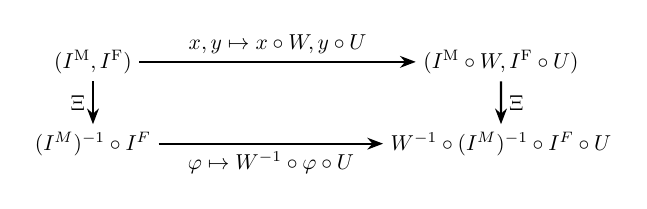
\begin{tikzpicture}[baseline=(current  bounding  box.center),scale=0.78, transform shape,node distance=.7 cm and 4.5cm, auto,
		every edge/.style={draw, -{Stealth[length=2mm]}, thick}]
		% Nodes
		\node (tl) {$(I^\text{M}, I^\text{F})$};
		\node (tr) [right=of tl] {$(I^\text{M} \circ W, I^\text{F} \circ U)$};
		\node (bl) [below=of tl] {$(I^M)^{-1} \circ I^F$};
		\node (br) [below=of tr] {$W ^{-1} \circ (I^M)^{-1} \circ I^F \circ U$};

		% Edges
		\draw (tl) edge node[above] {$x, y \mapsto x \circ W, y \circ U$} (tr);
		\draw (tl) edge node[left] {$\Xi$} (bl);
		\draw (tr) edge node[right] {$\Xi$} (br);
		\draw (bl) edge node[below] {$\varphi \mapsto W^{-1} \circ \varphi \circ U$} (br);
	\end{tikzpicture}
\end{equation}
\noindent
Now, if we have a new registration algorithm $\Phi$, a class of input images and potential transforms, we can check if that particular network is equivariant by checking if for all $W$, $U$ a diagram matching \ref{eqn:equivarianceproperty} holds (if so, the registration algorithm is $[W,U]$ equivariant w.r.t. diffeomorphisms):
\begin{equation}
	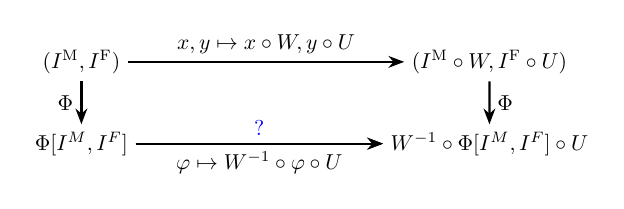
\begin{tikzpicture}[baseline=(current  bounding  box.center),scale=0.78, transform shape,node distance=.7 cm and 4.5cm, auto,
		every edge/.style={draw, -{Stealth[length=2mm]}, thick}]

		% Nodes
		\node (tl) {$(I^\text{M}, I^\text{F})$};
		\node (tr) [right=of tl] {$(I^\text{M} \circ W, I^\text{F} \circ U)$};
		\node (bl) [below=of tl] {$\Phi[I^M , I^F]$};
		\node (br) [below=of tr] {$W ^{-1} \circ \Phi[I^M , I^F] \circ U$};

		% Edges
		\draw (tl) edge node[above] {$x, y \mapsto x \circ W, y \circ U$} (tr);
		\draw (tl) edge node[left] {$\Phi$} (bl);
		\draw (tr) edge node[right] {$\Phi$} (br);
		\draw (bl) edge node[below] {$\varphi \mapsto W^{-1} \circ \varphi \circ U$} (br);        \draw (bl) edge node[above] {{\color{blue}?}} (br);
	\end{tikzpicture}
\end{equation}
In other words, if the registration algorithm results in $\varphi$ for registering $I^{\text{M}}$ to $I^\text{F}$, then it needs to be constructed such that it results in $W^{-1}\circ\varphi\circ U$ if images $I^{\text{M}}$ and $I^{\text{F}}$ are warped by $W$ and $U$, respectively. In that case, $W$ and U will not change the image correspondences.
%We say that a registration algorithm is [W, U] equivariant with respect to
%diffeomorphisms if it obeys that diagram. 

\vskip1ex
In practice, we will often restrict the group from which $W$ and $U$ may be chosen. For example, if for a registration algorithm
$\Phi$, for any translations $W$ and $U$, $\Phi[\ia \circ W, \ib \circ U] =
	W^{-1} \circ \Phi[I^M, I^F] \circ U$, we say that the algorithm $\Phi$ is $[W, U]$
equivariant with respect to translations.

\vskip1ex
Finally, we remark that some registration algorithms
are only equivariant for applying the same transform to both images; that is,
for any transform $U$ from a group of transforms $\mathcal{T}$, $\Phi[\ia \circ
		U, \ib \circ U] = U^{-1} \circ \Phi[I^M, I^F] \circ U$. We say that such an
algorithm is $[U, U]$ equivariant with respect to $\mathcal{T}$. This justifies the definitions we previewed in Sec.~\ref{section:notation}.
%From a practical perspective, a $[U,U]$ equivariant registration network will preserve correspondences under the \emph{same} transformations for the source and target images. Whereas, $[W,U]$ is more general and allows different deformations for the source and target images. In both cases, we know that the resulting map produced by the registration network changes such that spatial point correspondences between images are preserved.

\section{Coordinate attention}
%$\Xi_\theta$: a coordinate attention block than can handle real images}
\label{sec:coordinate_attention_block}

Our central contribution when seeking to realize $[W,U]$ equivariance is what we call \emph{coordinate attention}, \ie, a standard attention block where the value vectors are the coordinates of each voxel. This has the effect of computing the center of mass of the attention mask associated with each query. %, and allows this center of mass computation to be performed using highly optimized kernels, such as flash attention \cite{dao2022flashattention}. 
As an illustrative example in Appendix \ref{subsection:xinetimplementation}, we use coordinate attention to solve the diffeomorphism-to-diffeomorphism registration problem.



\begin{figure}
	\centering
	%\includegraphics[width=.94\columnwidth]{Xi_real_rk.pdf}
	\includegraphics[width=.99\columnwidth]{Xi_theta.drawio.pdf.drawio.pdf}
	\caption{Architecture of $\Xi_\theta$. The specific arrangement of pads and crops allows voxels to be mapped to points outside of $\Omega$ -- this is necessary to represent translation. 
		%$\Xi_\theta$ is similar to $\Xi_\mathcal{F}$ from Fig. \ref{xinet} but the pointwise sinusoidal embedding is replaced by a convolutional encoder. This restricts the class of transforms with respect to which $\Xi_\theta$ is equivariant: while the pointwise sinusoidal embedding of intensity used in $\Xi_\mathcal{F}$  is equivariant to arbitrary diffeomorphisms, the chosen convolutional network in $\Xi_\theta$ is only forced to be equivariant to translations. With this change, there is no longer a requirement that the input images are diffeomorphisms.
	}
	\label{fig:xitheta}
\end{figure}

\vskip0.5ex
For registering medical images, we use an architecture we call $\Xi_\theta$, a combination of coordinate attention with a feature encoder consisting of convolutional layers all operating at the same resolution, some of which are dilated. The encoder is exactly equivariant to integer pixel translations.
%and so coordinate attention with this convolutional encoder, which we call $\Xi_\theta$, is $[W, U]$ equivariant with respect to integer translation where $\Xi_\mathcal{F}$ was to arbitrary diffeomorphisms. 
Edge effects are reduced by padding with zeros before running
images through the feature encoder, and cropping afterwards. The architecture is illustrated in Fig.~\ref{fig:xitheta}. %\textcolor{blue}{(rk: integer)}
%By turning images into features using a translationally equivariant network such as stylegan3's alias free convolution, the resulting network is [W, U] equivariant with respect to translation. If we use a rotationally equivariant network such as spherical harmonic convolution, the resulting registration algorithm is [W, U] equivariant with respect to rigid motions.
It is important that the coordinate attention formulation, which is ``center of mass of $\text{softmax}(QV^\top)$'', can be computed using a standard attention operation instead of a custom set of operations on all pairs of feature vectors. Attention has heavily optimized implementations such as
flash attention~\cite{dao2022flashattention} that only require $\mathcal{O}$(\#voxels) memory and have excellent
cache coherency. While flash attention is $\mathcal{O}$(image side length$^6$),
in practice performance is adequate
%\footnote{Approximately 2.5 trillion operations} 
in our setting when $\Xi_\theta$ is applied to a volume of size $43 \times 43 \times 43$,
which is sufficient for coarse registration. We will show (in Sec.~\ref{twostepproof}) that it is then possible to
add fine-grained registration while preserving $[W, U]$ equivariance. 
\section{Equivariance of Coordinate Attention with convolutional encoders (\texorpdfstring{$\Xi_\theta$)}{XiTheta}}
\label{sec:wuproof}
We assume that the attention mask associated with each query vector has small spatial
support. Finding a training procedure that reliably fulfilled this assumption across different datasets was nontrivial: we find that this assumption is satisfied after regularizing the  network end-to-end with diffusion
regularization for the first several epochs, and using GradICON regularization thereafter. %This is a crucial empirical result that will be a subject of future research and analysis.

We assume that the feature encoders are translation equivariant like
\begin{equation}
	\convo_\theta(I \circ U) = \convo_\theta(I) \circ U
	\label{convdef}\,.
\end{equation}
With these assumptions, we prove that $\Xi_\theta$ is $[W, U]$ equivariant to translations below.

Without positional embeddings or causal masking, (we do not use
either) the attention mechanism is equivariant to permutations as follows: for $P_1, P_2$ permutations; and the output and $K$ (Key), $Q$ (Query), and $V$ (Value) inputs represented each as a function from an index to a vector, and an attention block represented as $\mathbb{T}$,
\begin{equation} \mathbb{T}[K \circ P_1, Q \circ P_2, V \circ P_1] = \mathbb{T}[K, Q, V] \circ P_2\,. \label{transperm}\end{equation}
Additionally, because the attention weights in an attention block sum to 1, for an affine function $f$, we have 
\begin{equation}\mathbb{T}[K, Q, f\circ V] = f \circ \mathbb{T}[K, Q, V]\,. \label{transaff}\end{equation}
A translation $W$ by an integer number of voxels is both affine when seen as an operation on coordinates, $W_{x \mapsto x + r}$, and a permutation of the
voxels when seen as an operation on voxel images $W_{\text{permutation}}$ (as long as we can neglect boundary effects). The map from indices to coordinates, $\text{coords}$, serves as the bridge between these two representations of a transform ($W_{x \mapsto x + r} \circ \text{coords} = \text{coords} \circ W_{\text{permutation}})$. As long as the attention masks have small spatial support, we can suppress boundary effects by padding with zeros before applying the operation. So, for translations $W$ and $U$, we have
\[\Xi_\theta[ I^M, I^F] :=\mathbb{T}[\convo_\theta (I^M ) , \convo_\theta(I^F), \text{coords}]\enspace, \]
from which we establish that $\Xi_\theta$ is $[W, U]$ equivariant with respect to translation as follows: 
\begin{equation}
	\begin{split}
       %& \Xi_\theta[ I^M, I^F] :=\mathbb{T}[\convo_\theta (I^M ) , \convo_\theta(I^F), \text{coords}]          \\
       %& \text{and then}
       %\\
		& \Xi_\theta[ I^M \circ W, I^F \circ U]  \\
        & =\mathbb{T}[\convo_\theta (I^M \circ W) , \convo_\theta(I^F \circ U), \text{coords}]          \\
		& \stackrel{\eqref{convdef}}{=} \mathbb{T}[\convo_\theta (I^M) \circ W , \convo_\theta(I^F) \circ U, \text{coords}] \\
		& \stackrel{\eqref{transaff}}{=} W^{-1} \circ \mathbb{T}[\convo_\theta (I^M) \circ W, \convo_\theta(I^F) \circ U, W \circ \text{coords}] \\
		& = W^{-1} \circ \mathbb{T}[\convo_\theta (I^M) \circ W, \convo_\theta(I^F) \circ U, \text{coords} \circ W]  \\
		& \stackrel{\eqref{transperm}}{=} W^{-1} \circ \mathbb{T}[\convo_\theta (I^M), \convo_\theta(I^F) \circ U, \text{coords}] \\
		& \stackrel{\eqref{transperm}}{=}  W^{-1} \circ \mathbb{T}[\convo_\theta (I^M), \convo_\theta(I^F), \text{coords}] \circ U \\
		& =  W^{-1} \circ \Xi_\theta[ I^M , I^F] \circ U\,.
	\end{split}
\end{equation}
The same argument can also be applied to $[W, U]$ equivariance to axis aligned $\pi$ or $\frac{\pi}{2}$ rotations, provided that $\convo_\theta$ is replaced with an appropriate rotation equivariant encoder.



\subsection{\texorpdfstring{$[U, U]$}{[U,U]} equivariance}
\label{sec:uu_equivariance}
So far, we have pointed out that $\Xi_\theta$ is $[W, U]$ equivariant to translation. Our next goal is to show that our full approach, \emph{Coordinate Attention with Refinement Layers} (CARL), is also $[W, U]$ equivariant to translation. To this end, we (1) show that VoxelMorph-like networks are $[U, U]$ equivariant to translation as they predict displacements, and then (2) show that a multi-step registration algorithm where the first step is $[W, U]$ equivariant and subsequent steps are $[U, U]$ equivariant is overall $[W, U]$ equivariant. Notably, any all-convolutional network is translationally equivariant% as can be seen from the following diagram
\footnote{At
	least, for translations of integer multiples of the least common multiple of all convolution
	strides, and considering the input and output of the convolution to be
	functions.}:
\begin{equation}
	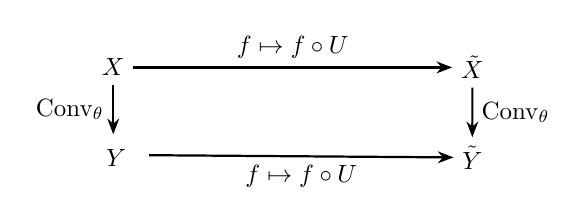
\begin{tikzpicture}[baseline=(current  bounding  box.center),scale=0.9, transform shape,node distance=.7cm and 4.5cm, auto,
		every edge/.style={draw, -{Stealth[length=2mm]}, thick}]
		% Nodes
		\node (tl) {$X$};
		\node (tr) [right=of tl] {$\tilde{X}$};
		\node (bl) [below=of tl] {$\phantom{\hat{Y}}$$Y$\hspace{-0.2cm} $\phantom{\hat{Y}}$};
		\node (br) [below=of tr] {$\tilde{Y}$};
		% Edges
		\draw (tl) edge node[above] {$f \mapsto f \circ U$} (tr);
		\draw (tl) edge node[left] {$\text{Conv}_\theta$} (bl);
		\draw (tr) edge node[right] {$\text{Conv}_\theta$} (br);
		\draw (bl) edge node[below] {$f \mapsto f \circ U$} (br);
	\end{tikzpicture}
	\label{eqn:convequi}
\end{equation}
To apply a convolutional network to registration, first it is made to have two inputs by channel-wise concatenation (cat), and it is chosen to have $D$ output channels. Its output can then be interpreted (via interpolation) as a function from the domain of the input images to $\mathbb{R}^N$. If used to predict coordinates, this has a different equivariance than $[U, U]$ equivariance: to be $[U, U]$ equivariant with respect to translation, a registration algorithm needs to have a bottom arrow $f \mapsto U^{-1} \circ f \circ U$ where Eq.~\eqref{eqn:convequi} has $f \mapsto f \circ U$. This is ameliorated in Quicksilver~\cite{yang2017quicksilver}, VoxelMorph~\cite{balakrishnan2019voxelmorph} and their successors by predicting displacements instead of coordinates. Overall, in VoxelMorph we have
\begin{equation}
	\Phi_\theta[\ia, \ib](\vec{x}) := \text{Conv}_\theta[\text{cat}(\ia, \ib)](\vec{x}) + \vec{x}\enspace,
\end{equation}
and by parameterizing our translation transform $U$ by a vector $\vec{r}$, we can compute
\begin{equation}
	\begin{split}
		\Phi_\theta&[\ia  \circ U, \ib \circ U](\vec{x}) \\ &= \text{Conv}_\theta[\text{cat}(\ia \circ U, \ib \circ U)](\vec{x}) + \vec{x}                       \\
		&= \text{Conv}_\theta[\text{cat}(\ia, \ib) \circ U](\vec{x}) + \vec{x}      \\
		&= \left(\text{Conv}_\theta[\text{cat}(\ia, \ib)] \circ U\right)(\vec{x}) + \vec{x}                  \\
		&= \text{Conv}_\theta[\text{cat}(\ia, \ib)](U(\vec{x})) + \vec{x}                         \\
		& = \text{Conv}_\theta[\text{cat}(\ia, \ib)](U(\vec{x})) + (\vec{x} + \vec{r}) - \vec{r}              \\
		&= U^{-1} \circ \left(\text{Conv}_\theta[\text{cat}(\ia, \ib)](\vec{x}) + \vec{x} \right) \circ U  \\ &= U^{-1} \circ \Phi_\theta[\ia, \ib](\vec{x}) \circ U\enspace.
	\end{split}
\end{equation}
%Hence, we see that predicting displacement fields results in $[U,U]$ equivariance while predicting coordinates would not.
\subsection{Two-step registration}
\label{sec:two_step_registration}
\label{twostepproof}
Multi-step registration is common practice, often using multiple algorithms. For example, ANTs \cite{avants2008symmetric} by default performs affine, then deformable registration, and returns the composition of the resulting transforms. Greer \etal~\cite{greer2021icon} propose a general notation for this scheme: the TwoStep operator, which takes as input two registration algorithms, and yields a composite algorithm as follows:
\begin{align}\text{TwoStep}&\{\Phi, \Psi\}[I^M, I^F] \nonumber \\ &= \Phi[I^M, I^F] \circ \Psi[I^M \circ \Phi[I^M, I^F], I^F]\,.\end{align}
%Assertion: if $\Phi$ is equivariant to transforming $I^M, I^F \rightarrow I^M \circ W, I^F \circ U$ (henceforth [W, U] equivariant) and $\Psi$ is equivariant to transforming $I^M, I^F \rightarrow I^M \circ U, I^F \circ U$ (henceforth [U, U] equivariant) for U and W from a class of transforms $\mathcal{T}$, then $TwoStep\{\Phi, \Psi\}$ is $[W, U]$ equivariant
We show that if $\Phi$ is $[W, U]$ equivariant and $\Psi$ is $[U, U]$ equivariant for $U,W$
from a class of transforms $\mathcal{T}$, then $\text{TwoStep}\{\Phi, \Psi\}$ is
$[W, U]$ equivariant. In particular, application of the definition of $\Phi$ being $[W, U]$ equivariant, see Eq.~\eqref{eqn:WUequiv}, and $\Psi$ being $[U, U]$ equivariant, see Eq.~\eqref{eqn:UUequiv}, yields
\begin{equation}
	\begin{split}
		& \text{TwoStep}\{\Phi, \Psi\}[I^M \circ W, I^F \circ U]  \\                 
		& \vspace{0.5cm}= \Phi\left[I^M \circ W, I^F \circ U\right] \circ \\
        & \vspace{0.5cm}\phantom{=~} \Psi\left[I^M \circ W \circ \Phi[I^M \circ W, I^F \circ U], I^F \circ U\right] \\
        & \vspace{0.5cm}\stackrel{\eqref{eqn:WUequiv}}{=} W^{-1} \circ \Phi[I^M, I^F] \circ U \circ \\
        & \vspace{0.5cm}\phantom{=~} \Psi\left[I^M \circ \Phi[I^M, I^F] \circ U, I^F \circ U\right] \\
        & \vspace{0.5cm}\stackrel{\eqref{eqn:UUequiv}}{=} W^{-1} \circ \Phi[I^M, I^F] \circ \\ 
        & \vspace{0.5cm}\phantom{=~} \Psi\left[I^M \circ \Phi[I^M, I^F], I^F\right] \circ U \\
        &  \vspace{0.5cm}=W^{-1} \circ \text{TwoStep}\{\Phi, \Psi\}[I^M, I^F] \circ U\enspace.
    \end{split}
\end{equation}
% \begin{equation}
% 	\begin{split}
% 		& \text{TwoStep}\{\Phi, \Psi\}[I^M \circ W, I^F \circ U]                                                                        \\
% 		& = \Phi[I^M \circ W, I^F \circ U] \\&\circ \Psi\left[I^M \circ W \circ \Phi[I^M \circ W, I^F \circ U], I^F \circ U\right] \\
% 		%& = W^{-1} \circ \Phi[I^M, I^F] \circ U \circ  \Psi\left[I^M \circ W \circ W^{-1} \circ \Phi[I^M, I^F] \circ U, I^F \circ U\right]
%         &\text{(apply definition of $\Phi$ being [W, U] equivariant)}\\
% 		& = W^{-1} \circ \Phi[I^M, I^F] \circ U \circ \Psi\left[I^M \circ \Phi[I^M, I^F] \circ U, I^F \circ U\right]            \\
% 		%& = W^{-1} \circ \Phi[I^M, I^F] \circ U \circ U^{-1} \circ \Psi\left[I^M \circ \Phi[I^M, I^F], I^F\right] \circ U                                                        \\
%         &\text{(apply definition of $\Psi$ being [U, U] equivariant)}\\
% 		& = W^{-1} \circ \Phi[I^M, I^F] \circ \Psi\left[I^M \circ \Phi[I^M, I^F], I^F\right] \circ U                            \\
% 		& = W^{-1} \circ \text{TwoStep}\{\Phi, \Psi\}[I^M, I^F] \circ U\enspace.
% 	\end{split}
% \end{equation}
%Therefore, $\text{TwoStep}\{\Phi, \Psi\}$ is $[W, U]$ equivariant. 
This construction can be applied recursively for an $N$-step $[W, U]$ equivariant network, and can be combined with the downsampling operator (abbreviated as Down) from \cite{tian2022} (see Appendix \ref{downsample}) to make the early stages operate at coarse resolution and subsequent ones at higher resolutions.

%\subsection{Resolution constraints}
%In 3D, the Equitrans network has computational complexity O(resolution \^6 ), and so can only operate on images up to around 40 x 40 x 40 in 3D, while VoxelMorph-like networks have complexity O(resolution \^3) and so can operate on high resolution medical images, in practice up to ~200 x 200 x 200. Therefore, this hybrid network provides a method for creating a [W, U] equivariant network that operates on 200 x 200 x 200 images, a capacity that would otherwise not be possible.

\section{Experiments}
\label{sec:experiments}
\noindent
\textbf{Architecture.} We propose the architecture \emph{Coordinate Attention with Refinement Layers} (CARL),
\begin{tcolorbox}[top=0mm,bottom=0mm,boxsep=1mm,colback=red!5!white,colframe=red!75!black]
	\begin{align}
		\text{CARL}   & :=\text{TwoStep}\{\text{TwoStep}\{ \text{Down}\{ \text{TwoStep} \{ \nonumber \\
		              & \text{Down} \{  \Xi_\theta\}\}, \Psi_1\}\}, \Psi_2 \nonumber                 \\
		\}, \Psi_3 \} &
		\label{eqn:CARL}
	\end{align}
\end{tcolorbox}
\noindent
where $\Xi_\theta$ is a $[W, U]$ equivariant neural network composed of a
translation-equivariant feature encoder and a coordinate attention layer as proposed, and
$\Psi_i$ are refinement layers: convolutional networks predicting displacements with architecture and feature counts from \cite{greer2021icon, tian2022}, and so are $[U, U]$ equivariant. To facilitate a direct comparison of performance, the specific arrangement of TwoStep and Downsample layers is identical to GradICON: our only change is to replace the lowest resolution displacement predicting network with $\Xi_\theta$. Following the suggestion of GradICON \cite{tian2022}, the final refinement layer $\Psi_3$ is only added after the first 50,000 steps of training. \emph{The overall network is
	$[W, U]$ equivariant with respect to translation.}

\vskip1ex
\noindent
\textbf{Losses.} In all experiments, we train with LNCC image similarity (LNCC=1-local normalized cross correlation). For regularization, we train initially with a diffusion loss for 1,500 steps, \ie,
\begin{equation}
\begin{split}
	\mathcal{L} & = \text{LNCC}\left(I^\text{M} \circ \text{CARL}[\ia, \ib], \ib\right)  \\ &+  \text{LNCC}\left(I^\text{F} \circ \text{CARL}[\ib, \ia], I^\text{M}\right) \\&+ \lambda ||\nabla (\text{CARL}[\ia, \ib]) - \mathbf{I} ||_F^2
    \end{split}
\end{equation}
and then continue training with the GradICON \cite{tian2022} regularizer for 100,000 steps, \ie,
\begin{equation}
\begin{split}
\mathcal{L} & =  \text{LNCC}(I^M \circ \text{CARL}[\ia, \ib], \ib)  \\&+  \text{LNCC}(I^F \circ \text{CARL}[\ib, \ia], I^M)  \\&+ \lambda ||\nabla (\text{CARL}[\ia, \ib] \circ \text{CARL}[\ib, \ia]) - \mathbf{I} ||_F^2\,,
              \label{gradicon_loss}
\end{split}
\end{equation}
where $\mathbf{I}$ is the identity matrix, and $\lambda>0$.
We use regularization parameter $\lambda = 1.5$ and an Adam optimizer with a learning rate of 0.0001. We remark that diffusion regularization is needed in early steps of training for stability, but \text{GradICON} delivers superior final regularity and correspondence by strongly forcing the network towards invertibility while still allowing large deformations.
\vskip1ex
\noindent
\textbf{Instance Optimization (IO).} Following GradICON~\cite{tian2022}, we evaluate with and without 50 steps of Instance Optimization, \ie, since our method does not use human annotations at train time, at deployment we can further optimize Eq.~\eqref{gradicon_loss} on instances of test data to improve performance.

\subsection{Deformed retina images}
\label{retinaexpr}
We first demonstrate the importance of several details of
our implementation on a dataset consisting of synthetically warped retina
segmentations from \cite{tian2022}. In particular, for this experiment,
we train three network variants:
\begin{itemize}
	\item[1)] $\text{TwoStep}\{\text{Down}\{\text{TwoStep}\{\text{Down}\{\Psi_0\},\Psi_1\}\}, \Psi_2 \}$, a multi-step network with each step predicting a displacement field. This is the 1st stage architecture proposed in GradICON~\cite{tian2022}. We expect this network to \emph{not} be $[W, U]$ equivariant w.r.t. translation.
	\item[2)] $\text{Down}\{\text{Down}\{\Xi_\theta\}\}$, a single-step coordinate attention network . We expect this network to be $[W, U]$ equivariant w.r.t translation, but less powerful than 1).
	\item[3)] CARL, Eq.~\eqref{eqn:CARL}. We expect this  network to be powerful and $[W, U]$ equivariant to translation.
\end{itemize}
Each is assessed \emph{without} instance optimization. To assess differences between these network types, we create three variants of the retina dataset:
\begin{itemize}
	\item[1)] {\bf Baseline}. The train
		set is constructed by warping 14 segmentations from the DRIVE dataset \cite{staal2004ridge}, and the
		test set is constructed by warping the remaining 6 segmentations, with elastic warp parameters as suggested in~\cite{tian2022}.
	\item[2)] {\bf Shift}. The same as Baseline, but with fixed images shifted by 200 pixels ($\sim \frac{1}{3}$ of retina diameter).
	\item[3)] {\bf Scale Shift}. The same as Shift, but with fixed images also scaled to 80\% size (See Fig. \ref{fig:synthetic_experiment}).
\end{itemize}

\vskip0.5ex
\noindent
Results for this experiment are shown in Fig.~\ref{fig:synthetic_experiment}. We see that when training/testing on the \textbf{Baseline} dataset, as expected, all three networks have adequate performance, although the importance of the refinement layers is highlighted when $\text{Down}\{\text{Down}\{\Xi_\theta\}\}$ falls meaningfully behind. When trained and tested on the \textbf{Shift} variant, the equivariant networks succeed, while the displacement predicting network fails. Additionally, we see that the equivariant networks \emph{generalize} to the \textbf{Shift} test dataset when trained only on \textbf{Baseline}. Finally, we see that the equivariant networks also learn on, \emph{and generalize to}, the \textbf{Scale Shift} dataset. This result illustrates an important point that we did not prove but observe empirically: while $\Xi_\theta$ is formally only $[W, U]$ equivariant to integer translations, in practice it is $[W, U]$ equivariant to deformations that are locally approximately translations, such as scaling. We do see a large variance \textbf{between training runs} when training CARL on the \textbf{Shift} and \textbf{Scale Shift} datasets. That is, specifically when training on Shift or Scale Shift, most trained CARL networks have high performance across all test examples, but for a small fraction of training runs, performance is poor across the whole test set.

\begin{figure*}[t!]
\centering
\includegraphics[width=1.0\textwidth]{Figures/CVPR_Fig3_rk.pdf}
\caption{\label{fig:synthetic_experiment}Equivariance allows CARL to generalize out-of-distribution. The \emph{left four images} show the performance of CARL on a test set with the same distribution as the training set, where images are \emph{aligned} in scale and translation. The \emph{middle four images} show generalization to a test set \textbf{Scale Shift} where images are \emph{misaligned} in scale and translation. The \emph{right-most} figure shows the mean Dice distribution on the test set, over multiple training runs.}
\vskip-0.5em
\end{figure*}

% \begin{figure}
% 	\centering
% 	\includegraphics[width=.8\columnwidth, trim={0cm 0cm 23.2cm 0cm}, clip]{Figures/retina_rk.pdf}\\
% 	\includegraphics[width=.8\columnwidth, trim={10.5cm 0cm 12.8cm 0cm}, clip]{Figures/retina_rk.pdf}\\
% 	\includegraphics[width=.8\columnwidth, trim={20.6cm 0cm -.3cm 0cm}, clip]{Figures/retina_rk.pdf}
% 	%\includegraphics[width=\columnwidth, trim={2cm 1cm 2cm 1cm}, clip]{Figures/038_hard_mode_generalize_make_hybrid_network_after_registration.png}
% 	%\includegraphics[width=.28\textwidth, trim={2cm 1cm 2cm 1cm}, clip]{Figures/039_hard_mode_generalize_make_hybrid_network_test.png}
% 	%\includegraphics[width=.4\textwidth]{Figures/000_violin.png}
% 	\caption{Equivariance allows CARL to generalize out-of-distribution. The \emph{top} figure shows the performance of CARL on a test set with the same distribution as the training set, where images are \emph{aligned} in scale and translation. The \emph{middle} figure shows generalization to a test set \textbf{Scale Shift} where images are \emph{misaligned} in scale and translation. The \emph{bottom} figure shows the mean Dice distribution on the test set, over multiple training runs.
% 		%There are defects in the transform away from the center of the image which/ can be fixed by increasing the padding.
% 	}
% 	\vskip-0.5em
% \end{figure}

\subsection{Performance comparison to other methods}
We compare our method to existing approaches from the literature on three datasets. First, we
evaluate on the 10 DirLab COPDGene test cases as this is a popular and
difficult lung registration benchmark that allows us to compare our performance to
diverse and highly optimized methods. Second, we evaluate on the HCP brain
dataset, which allows us to directly compare to two existing equivariant
registration methods, EasyReg and KeyMorph. Third, we evaluate on a novel
registration task: registering images from the Abdomen1k dataset without
registration-specific preprocessing. This dataset has large translational
differences and different fields of view, which causes other unsupervised
registration approaches to converge poorly. Our strong equivariance makes this
task possible with the LNCC + regularization loss. We aim to present a picture of how our approach will work when applied as specified to new datasets. To this end, \emph{we use the same hyperparameters for all three datasets}.


\vskip0.5ex
\noindent
\textbf{Lung registration.}
To evaluate CARL against the current state of the art for general registration, we use the DirLab lung registration task, which is well standardized and has gained considerable attention in the community. In particular, we train on 999 inhale/exhale CT pairs of images from the COPDGene dataset, and evaluate based on landmark distance in the 10 standard DirLab pairs. We follow the data preparation and augmentation suggested in GradICON~\cite{tian2022}. Results are listed in Table~\ref{tab:exp_results}, showing the commonly-used mean target registration error (mTRE) score as well as the percentage of negative values for the Jacobian determinant ($\%|J|_{<0}$), indicative of the number of folds. Performance matches state of the art, exceeded significantly only by PTVReg and RRN which have hyper parameters selected specifically for the 10 challenge cases.%Results marked by (io) indicate an additional \emph{instance optimization} step. 

\vskip1ex
\noindent
\textbf{Brain registration.}
\label{brainreg}
The existing equivariant registration methods that we compare to are presented as brain registration methods. We compare to them on T1w MRI images from the Human Connectome Project (HCP) dataset~\cite{van2012human,rushmore2022anatomically,rushmore_r_jarrett_2022_dataset}. In detail, we perform evaluation and preprocessing as in \cite{greer2023inverse}, measuring DICE of midbrain structures \ref{fig:box_hcp} and find that CARL yields state-of-the-art performance. We also artificially translate or rotate one image by varying amounts and re-evaluate performance, verifying that GradICON sharply drops in performance under this shift, while our approach and EasyReg are unaffected (see Fig.~\ref{fig:hcp_translation}).

\vskip1ex
\noindent
\textbf{Abdomen registration.}
Abdominal CT-CT datasets can capture the diversity of fields of view of abdominal CT
scans in clinical practice, and the Abdomen1k~\cite{Abdomen1K9497733} dataset is curated specifically to do so. Since our method is robust to these differences of
field of view because it is $[W, U]$ equivariant to translation, we showcase its
performance for inter-subject registration of the Abdomen1K \cite{Abdomen1K9497733} dataset. We train on the first 800 cases of the Abdomen1K dataset, validate on cases 900-1000, and test on cases 800-900. We opt for a minimalist preprocessing: we resample all images to [175, 175, 175]
\footnote{This leads to nonisometric voxel spacing. We tried isometric voxel spacing, padding with background pixels if necessary, but non-isometric, non padded preprocessing had uniformly better performance}
and then divide by the maximum intensity. We test by randomly sampling 30 image pairs and then computing the mean Dice score over manual annotations of the liver, kidney, pancreas, and spleen. We report (Appendix, \ref{abdomen_fulldata}) the exact pairs to allow future works to compare to our result. The most important comparison is to {GradICON}, as our final network, similarity and regularity loss are identical to GradICON's except that we  replace the first U-Net based $\Psi$ with our custom $\Xi_\theta$. This change produces a dramatic improvement in non-instance-optimization registration accuracy and an improvement in instance-optimized registration accuracy. Results are listed in Table \ref{tab:exp_results}. We also check whether the model trained on the Abdomen1k dataset generalizes to the Learn2Reg Abdomen CT-CT challenge set \cite{hering2022learn2reg}. We find excellent generalization: performance is better than other unsupervised approaches including the keypoint-based SAME++, but does not match the best supervised methods trained using the Learn2Reg CT-CT training set \emph{and segmentations}.

\begin{table*}[htp]
	\centering
	\captionof{table}{Performance comparison on Abdomen1K, HCP, DirLab, and Learn2Reg Abdomen CT-CT dataset.}\label{tab:exp_results}
	\vskip0.1ex
	\begin{adjustbox}{width=\textwidth,center}
		\begin{tabular}{lccp{1em}lccp{1em}lcc}\toprule
			Method                                                    & $\%$DICE$\uparrow$ & $\%|J|_{<0}\downarrow$ & & Method                                                  & mTRE$\downarrow$ & $\%|J|_{<0}\downarrow$                        & & Method                                                        & $\%$DICE$\uparrow$ & Unsupervised \\ \midrule
			\multicolumn{3}{c}{\cellcolor[RGB]{205,224,238}Abdomen1K}                                           & & \multicolumn{3}{c}{\cellcolor[RGB]{255,228,206}DirLab}                                                                     & & \multicolumn{3}{c}{\cellcolor{blue!10}L2R Abd. CTCT Test set}                                              \\
			ANTs~\cite{avants2008symmetric}                           & 45.4           & 0                      & & ANTs~\cite{avants2008symmetric}                         & 1.79             & 0                                             & & ConvexAdam~\cite{siebert2021fast}                             & 69             &                       \\
			VoxelMorph~\cite{balakrishnan2019voxelmorph}              & 59.3           & -                      & & Elastix~\cite{klein2009elastix}                         & 1.32             & -                                             & & LapIRN~\cite{mok2020large}                                    & 67             &                       \\
			GradICON~\cite{tian2022}                                  & 49.6           & 7e-1                   & & VoxelMorph~\cite{balakrishnan2019voxelmorph}            & 9.88             & 0                                             & & Estienne~\cite{estienne2021deep}                              & 69             &                       \\
			GradICON(IO)~\cite{tian2022}                              & 71.0           & 4e-2                   & & LapIRN~\cite{mok2020large}                              & 2.92             & 0                                             & & corrField~\cite{hansen2021graphregnet,heinrich2015estimating} & 49             & yes                             \\
			ConstrICON~\cite{greer2023inverse}                        & 65.2           & 7e-4                   & & RRN~\cite{he2021recursive}                              & 0.83             & -                                             & & PIMed~\cite{hering2022learn2reg}                              & 49             &                              \\
			ConstrICON(IO)~\cite{greer2023inverse}                    & 66.8           & 2e-3                   & & Hering el al~\cite{hering2021cnn}                       & 2.00             & 6e-2                                          & & PDD-Net~\cite{heinrich2019closing}                            & 49             &                              \\
			uniGradICON~\cite{tian2024unigradicon}                    & 43.5           & 9e-1                   & & GraphRegNet~\cite{hansen2021graphregnet}                & 1.34             & -                                             & & Joutard~\cite{hering2022learn2reg}                            & 40             &                              \\
			uniGradICON(IO)~\cite{tian2024unigradicon}                & 54.8              &    2e-3                   & & PLOSL~\cite{wang2022PLOSL}                              & 3.84             & 0                                             & & NiftyReg~\cite{modat2010fast}                                 & 45             & yes                             \\
			\textbf{CARL}                                             & 75.7           & 4e-1                   & & PLOSL(IO)~\cite{wang2022PLOSL}                          & 1.53             & 0                                             & & Gunnarsson~\cite{gunnarsson2020learning}                      & 43             &                              \\
			\textbf{CARL(IO)}                                         & 77.2           & 2e-3                   & & PTVReg~\cite{vishnevskiy2017isotropic}                  & 0.83             & -                                             & & \multicolumn{3}{c}{\cellcolor{blue!10}L2R Abd. CTCT Val. set}                                              \\
			\multicolumn{3}{c}{\cellcolor[RGB]{208,234,208}HCP}                                                 & & GradICON~\cite{tian2022}                                & 1.93             & 3e-4                                          & & ConvexAdam~\cite{siebert2021fast}                             & 71                                              \\
			ANTs~\cite{avants2008symmetric}                           & 77.2           & 0                      & & GradICON(IO)~\cite{tian2022}                            & 1.31             & 2e-4                                          & & Estienne~\cite{estienne2021deep}                              & 65                                              \\
			GradICON~\cite{greer2023inverse}                          & 78.6           & 1e-3                   & & ConstrICON~\cite{greer2023inverse}                      & 2.03             & 7e-6                                          & & Estienne~\cite{estienne2021deep}                              & 52             & yes                            \\
			GradICON(IO)~\cite{greer2023inverse}                      & 80.2           & 5e-4                   & & ConstrICON(IO)~\cite{greer2023inverse}                  & 1.62             & 3e-6                                          & & SAME++(IO)~\cite{Tian2023SAMEAS}                              & 49             & yes                            \\
			ConstrICON~\cite{greer2023inverse}                        & 79.3           & 4e-6                   & & uniGradICON~\cite{tian2024unigradicon}                  & 2.26             & 9e-5                                          & & uniGradICON    ~\cite{tian2024unigradicon}                    & 48             & yes                            \\
			ConstrICON(IO)~\cite{greer2023inverse}                    & 80.1           & 0                      & & uniGradICON(IO)~\cite{tian2024unigradicon}              & 1.40             & 9e-5                                          & & uniGradICON(IO)~\cite{tian2024unigradicon}                    & 52             & yes                            \\
			uniGradICON~\cite{tian2024unigradicon}                    & 76.2           & 6e-5                   & & \textbf{CARL}                                           & 1.88             & 4e-6                                          & & \textbf{CARL}                                                 & 50             & yes                            \\
			uniGradICON(IO)~\cite{tian2024unigradicon}                & 78.9           & 2e-4                   & & \textbf{CARL(IO)}                                       & 1.34             & 6e-6                                          & & \textbf{CARL(IO)}                                             & 56             & yes                            \\
			EasyReg~\cite{iglesias2023ready}                          & 78.8           & -                      & & \multicolumn{3}{c}{\cellcolor{white}}                                                                                      & & \multicolumn{2}{c}{\cellcolor{white}}                                                                           \\
			KeyMorph~\cite{Yu22a}                                     & 67.2           & 0                      & & \multicolumn{3}{c}{\cellcolor{white}}                                                                                      & & \multicolumn{2}{c}{\cellcolor{white}}       \\
                        \textbf{CARL}                                             & 79.6           & 6e-3                   & & \multicolumn{3}{c}{\cellcolor{white}}                                                                                      & & \multicolumn{2}{c}{\cellcolor{white}}\\ 
                        \textbf{CARL(IO)}                                         & 80.4           & 1e-3                   & & \multicolumn{3}{c}{\cellcolor{white}}                                                                                      & & \multicolumn{2}{c}{\cellcolor{white}}\\ 
                        \textbf{CARL\{ROT\}}                                      & 77.8           & 1e-3                   & & \multicolumn{3}{c}{\cellcolor{white}}                                                                                      & & \multicolumn{2}{c}{\cellcolor{white}}\\ 
                        \textbf{CARL\{ROT\}(IO)}                                  & 78.9           & 3e-3                   & & \multicolumn{3}{c}{\cellcolor{white}}                                                                                      & & \multicolumn{2}{c}{\cellcolor{white}}\\ 
   \bottomrule
		\end{tabular}
	\end{adjustbox}
	\vskip-0.1em
\end{table*}


\iffalse
	\noindent\begin{minipage}{0.4\textwidth}
		\centering
		\begin{small}
			\captionof{table}{Results on Abdomen1k. We outperform existing methods when input images are not approximately aligned in translation due to differing CT fields of view.}
			\label{tab:abdomen}
			\begin{tabular}{@{}lcc@{}}
				\toprule
				\textbf{Method}                                & \textbf{DICE} & $\%|J|_{<0}$ \\
				\midrule

				ANTs \cite{avants2008symmetric}                & 45.4          & 0            \\
				%ANTs Affine + SyNAggro                         & -- & -           \\
				%ANTs affine alignment using test labels        & -- & -           \\
				%ANTs affine test prealigned, then SyN          & 51.5 & 0           \\
				%        LapIRN                                                            \\
				VoxelMorph \cite{balakrishnan2019voxelmorph}                                  \\
				GradICON                       \cite{tian2022} & 49.6          & 0.7          \\
				GradICON (io)                                  & 71.0          & 4e-2         \\
				ConstrICON \cite{greer2023inverse}             & 65.2          & 7e-4         \\
				ConstrICON (io)                                & 66.8          & 2e-3         \\
				CARL -- \textbf{Ours}                          & 74.1          & 0.3          \\
				CARL (io) -- \textbf{Ours}                     & 75.9          & 4e-3         \\
				\bottomrule
			\end{tabular}
			% \vskip1ex
		\end{small}

	\end{minipage}\hfill
	\noindent\begin{minipage}{0.59\textwidth}
		\centering
		\begin{small}
			\captionof{table}{Results on DirLab (lung registration). Our method is comparable to the state of the art on an extremely competitive standard task.}
			\label{tab:dirlab}
			\begin{tabular}{@{}lcc|lcc@{}}
				\toprule
				\textbf{Method}                              & \textbf{mTRE} & $\%|J|_{<0}$ &
				\textbf{Method}                              & \textbf{mTRE} & $\%|J|_{<0}$                                                        \\
				\midrule
				ANTs    \cite{avants2008symmetric}           & 1.73          & 0            & PLOSL (io)                             & 1.53 & 0    \\
				Elastix \cite{klein2009elastix}              & 1.32          &              & PTVReg \cite{vishnevskiy2017isotropic} & 0.83 & --   \\
				VoxelMorph \cite{balakrishnan2019voxelmorph} & 9.88          & 0            & GradICON     \cite{tian2022}           & 1.93 & 3e-4 \\
				LapIRN     \cite{mok2020large}               & 2.92          & 0            & GradICON (io)                          & 1.31 & 2e-4 \\
				RRN           \cite{he2021recursive}         & 0.83          &              & ConstrICON \cite{greer2021icon}        & 2.06 & 6e-6 \\
				Hering \etal      \cite{hering2021cnn}       & 2.00          &              & ConstrICON (io)                        & 1.62 & 3e-6 \\
				GraphRegNet \cite{hansen2021graphregnet}     & 1.34          & --           & \text{CARL} -- \textbf{Ours}           & 2.58 & 2e-6 \\
				PLOSL \cite{wang2022plosl}                   & 3.84          & 0            & \text{CARL} (io) -- \textbf{Ours}      & 1.52 & 3e-6 \\
				\bottomrule
			\end{tabular}
			%\vskip1ex
		\end{small}
	\end{minipage}


	\noindent\begin{minipage}{0.4\textwidth}

		\centering
		\captionof{table}{Evaluation on HCP of multiple methods }
		\label{tab:HCP_overall}
		\begin{tabular}{@{}lcc@{}}
			\toprule
			Method                             & DICE & $\%|J|_{<0}$ \\
			\midrule
			ANTs \cite{avants2008symmetric}    & 77.2 & 0            \\
			GradICON \cite{tian2022}           & 78.6 & 1e-3         \\
			GradICON (io)                      & 80.2 & 5e-4         \\
			ConstrICON \cite{greer2023inverse} & 79.3 & 4e-6         \\
			ConstrICON (io)                    & 80.1 & 0            \\
			EasyReg\cite{iglesias2023ready}    & 78.8 & -            \\
			KeyMorph \cite{Yu22a}              &      &              \\
			CARL (ours)                        & 78.8 & 5e-4         \\
			CARL (io)                          & 80.4 & 3e-4         \\
			\bottomrule
		\end{tabular}

	\end{minipage} \hfill
\fi


\begin{figure}[htp]
	\centering
	\includegraphics[width=\columnwidth, trim={0cm 0cm 0cm 0.43cm}, clip]{Figures/translating_one_image.pdf}
	\includegraphics[width=\columnwidth, trim={0cm 0cm 0cm 0.43cm}, clip]{Figures/rotating_one_image.pdf}
	\caption{HCP evaluation while translating or rotating one image. CARL and EasyReg are unaffected by translation due to $[W,U]$ equivariance, and CARL\{ROT\} is additionally unaffected by rotation. GradICON DICE drops significantly when images are transformed differently due to its $[U,U]$ equivariance.}
	\label{fig:hcp_translation}
	\vskip-0.8em
\end{figure}

\subsection{Rotation equivariance}

Our approach is formally $[W, U]$ equivariant to translations. In addition, we find empirically that it can be made nearly $[W, U]$ equivariant to rotations by data augmentation. The following changes to the training procedure are required: \emph{First}, $\Xi_\theta$ is made formally equivariant to axis aligned $\pi$ rotations by evaluating the encoder four times, once for each possible $\pi$ rotation, and averaging. If the encoder is equivariant in the natural sense to transforms from a class $\mathcal{T}$, then $\Xi_\theta$ becomes $[W, U]$ equivariant to that class as mentioned in \ref{sec:coordinate_attention_block}. \emph{Second}, the receptive field of the encoder is broadened by adding an additional dilated convolution to the residual blocks with dilation 8. This empirically stabilizes training, but slightly damages translational equivariance via increased boundary effects. In addition, we change the extrapolation used when evaluating displacement field transforms at locations outside $[0, 1]$ (see \ref{sec:improved_extrapolation} in the Appendix). This change allows the Jacobian of the final transform to be continuous across this boundary when the displacement field represents a large rotation. \emph{Finally}, the dataset is augmented with random rotations from $\text{SO}(3)$. Because this augmentation requires large rotations to align the images, pretraining with naive diffusion regularization (\ie $\mathcal{L}_\text{reg}(\varphi) = ||\nabla \varphi - \boldsymbol{I}||^2_F$) is no longer appropriate as diffusion forbids transforms with Jacobians far from the identity map. During the pretraining step, it is therefore necessary to apply the diffusion regularizer to $R^{-1} \circ \varphi \circ Q$ instead of $\varphi$, where $R$ and $Q$ are the augmentations applied to the input images and $\varphi$ is the output of the overall architecture. As the network becomes $[W, U]$ equivariant to arbitrary rotations, $\nabla (R^{-1} \circ \varphi \circ Q)$ becomes close enough to the identity matrix for diffusion regularization to be appropriate: see \ref{sec:augmentation}. We refer to CARL trained using this procedure as CARL\{ROT\}. While baseline CARL can handle rotations of up to 45 degrees with instance optimization, CARL\{ROT\} performs correct registration when the input images are arbitrarily rotated (\ref{fig:hcp_translation}).

\subsection{Limitations}
\label{subsection:limitations}
%\vspace{-0.1cm}

%While we achieve theoretical and empirical equivariance to translation and empirical equivariance to scale, notably absent from our results are equivariance to rotations. This does not doom CARL, as our driving goal was to accurately register abdominal organs, where the rough rotation is known from the image metadata, and the driving issue is discrepancy in translation. For other areas of application, such as fetal MRI registration as tackled by E-CNN \cite{billot2023equivariant}, translation equivariance is much less important since moments-based initialization works well, and rotational equivariance takes foremost importance as the rough orientation of the fetus with respect to the scanner is initially unknown. Our derivation of $[W, U]$ equivariance to translation (Sec.~\ref{sec:wuproof}) holds for $[W, U]$ equivariance with respect to rotation if $\convo_\theta$ is replaced with a rotation equivariant encoder such as \cite{karras2021alias} or \cite{moyer2021equivariant}, but unlike for translation equivariant encoders, the assumption that attention maps should have small spatial support after training does not hold following any training procedure of a $\Xi_\theta$ with  rotationally equivariant encoders that we have attempted; a dedicated loss to encourage small spatial support may be required.

Registering a pair of images with a forward pass takes 2.1 seconds. Instance optimization (IO) is slower: 209 seconds on an NVIDIA A100 GPU. %, with the majority of this time spent computing flash attention forwards and backwards passes on an 80,000 token sequence
However, we consider the runtime of IO a minor issue at the moment, and focus on accuracy, as we anticipate that hardware and software for computing the flash attention kernel will continue to improve.

\section{Conclusion}
We demonstrated that our proposed multi-step architecture has a novel combination of strong equivariance (by construction to translation and optionally for rotation by judicious data augmentation) and precise handling of complex and high-resolution deformations. We show that it has close to SOTA accuracy on lung registration when compared to a competitive leaderboard, SOTA performance on brain registration with empirically verified equivariance to translations and rotations, and significantly improves registration accuracy over previous unsupervised registration approaches for the challenging registration of raw abdomen scans with differing fields of view. %Further, our approach has moderate memory consumption during training and testing ($\sim$25GB and $\sim$14GB respectively) and allows for fast inference.

% WARNING: do not forget to delete the supplementary pages from your submission 


%


\begin{figure*}[tp!]
    \centering
    \includegraphics[width=.96\textwidth]{Figures/unknown.png}
    \includegraphics[width=.43\textwidth]{Figures/box_label.png}
    \caption{Per structure DICE scores on the HCP dataset. CARL ranks well on most structures.}
    \label{fig:box_hcp}
\end{figure*}
\begin{figure*}[tp!]
    \centering
    \includegraphics[width=.96\textwidth]{Figures/abdomen_box.png}
    \includegraphics[width=.43\textwidth]{Figures/Abdomen_legent.png}
    \caption{Per structure DICE scores on the Abdomen1k dataset. We observe that CARL is dramatically ahead of competing methods on liver, kidney, and spleen registration, but performs meaninfully worse than Voxelmorph on the pancreas.}
    \label{fig:box_abd}
\end{figure*}

\section{Per Structure DICE Box Plot}
To provide a more comprehensive picture of how different registration algorithms perform for different brain structures or organs (instead of purely reporting averages) Figs.~\ref{fig:box_hcp} and~\ref{fig:box_abd} show anatomy-specific boxplots. We observe especially strong performance for CARL on the Abdomen1k dataset (Fig.~\ref{fig:box_abd}) with excellent registration results for liver, kidney, and spleen. 

\section{Resolution, Downsampling \& Coordinates}
\label{downsample}

We use an internal convention that regardless of resolution, images have coordinates ranging from (0, 0, 0) to (1, 1, 1). Thus, a transform, a function from $[0, 1]^D \rightarrow \mathcal{R}^N$, can be applied to an image of any resolution. This allows us to construct a multiresolution, multi-step registration algorithm using TwoStep and the operator Downsample defined in \cite{greer2021icon} as
\begin{align}
&\text{Downsample}\{\Phi\}[\ia, \ib] \nonumber \\
&= \Phi[ \text{averagePool}(\ia, 2), \text{averagePool}(\ib, 2)]\,. \\
&\text{TwoStep}\{\Phi, \Psi\}[I^M, I^F] \nonumber \\ &= \Phi[I^M, I^F] \circ \Psi[I^M \circ \Phi[I^M, I^F], I^F]\,.\end{align}

\section{Implementing the diffeomorphism-to-diffeomorphism case}
\label{subsection:xinetimplementation}

We can use coordinate attention to solve the diffeomorphism-to-diffeomorphism registration problem with a neural network $\Xi_\mathcal{F}$ (shown in the left part of Fig.~\ref{xinet}).

%$\Xi_\mathcal{F}$: an implementation of $\Xi$ using standard neural network components}

\begin{figure*}[htp]
    \centering
    %\includegraphics[width=.8\columnwidth]
 %{Figures/AnalyticalRegTransformer/closed form registration.drawio-1.pdf}
    \includegraphics[width=.5\textwidth]{Figures/AnalyticalRegTransformer/closed_form_registration.drawio-1.pdf}
    \includegraphics[width=.43\textwidth, trim={17cm 0cm 0cm 0cm}, clip]{Figures/AnalyticalRegTransformerPDF/M_F_Xi_rk.pdf}
    %\includegraphics[width=.99\columnwidth]{Figures/AnalyticalRegTransformerPDF/M_F_Xi_rk.pdf}
    \caption{\label{xinet}\emph{Left}: Neural network $\Xi_\mathcal{F}$ implementing $\Xi$. \emph{Right}: Result of registering the 1-dimensional "images" $\ia : [0, 1] \rightarrow[0, 1], x \mapsto \cos(\frac{\pi}{2} x)$ and $\ib : [0, 1] \rightarrow[0, 1], x \mapsto x + 0.07 \sin(3\pi x)$ via $\Xi$ and $\Xi_\mathcal{F}$, illustrating that the resulting maps are equivalent. $\Xi$ is computable here as these images are invertible and smooth. The neural network output (gold) closely matches the analytical solution (i.e., $\Xi[\ia, \ib] = \ia^{-1} \circ \ib = \frac{2}{\pi} \cos^{-1}(x + 0.07 \sin(3\pi x))$, gray).\label{Fig:analytincal} \emph{Best-viewed in color.}}
\end{figure*}
% %We will implement $\Xi := (\ia)^{-1} \circ \ib$ using conventional neural components. 
% Now, we introduce coordinate attention. Coordinate attention is simply a standard attention block where the value vectors are the coordinates of each voxel. This has the effect of computing the center of mass of the attention mask associated with each Query, and allows this center of mass computation to be performed using highly optimized kernels, such as flash attention.

The input functions $I^\text{M}$, $I^\text{F}$, and the output transform are approximated as arrays of voxels. The functional $\Xi$ such that $\Xi[I^M, I^F]:= (I^M)^{-1} \circ I^F$ (which only operates on images that are diffeomorphic) can be directly implemented, without training, using standard neural network components. We refer to this implementation as $\Xi_\mathcal{F}$. The intention is to map each voxel in the moving image into a high dimensional vector that will have a large dot product with the corresponding voxel in the fixed image with the same value, and then compute the attention matrix with the embedded fixed image voxels as the queries and the embedded moving image voxels as the keys. Subsequently, we can compute the center of mass of the attention masks (i.e., where each fixed image voxel matches on the moving image) by setting the \emph{values} to be the raw coordinates of the moving image voxels. We choose for the embedding a $1\times 1$ convolution with large weights followed by a sine-nonlinearity, which has the desired property of two vectors having a large dot product only when their input intensities are similar. Because our images are diffeomorphisms, we know a-priori that the input intensity of our moving image will only be close to intensities of the fixed image in a small region. We verify that this network, without any training, reproduces $\Xi$ when applied to input images that are diffeomorphisms, see~Fig.~\ref{Fig:analytincal} (right).
%with $\ia$ and $\ib$ represented as arrays of pixels containing image values (i.e., the standard representation) and the output transform represented as an array of coordinates. To do this, we need a representation of the identity map: two standard 1x1 convolution layers with shared weights, a $\sin$ nonlinearity, and an attention layer. In plain english, for each input Query an attention layer returns the average of all input Values, weighted by the similarity of their associated Keys to the Query. When this work applies attention, the Value vector is always the the (x, y, z) coordinate of that pixel in the fixed image, hence "Coordinate Attention". The weighted average of coordinates is a center of mass, and so each Query (generated by sampling the features of the encoded moving image) gets mapped to the center of mass of its match to the Key vectors associated with each pixel of the fixed image. This works after random weight initialization, without training, for 1-d images that are diffeomorphisms (\ref{Fig:analytincal}). Because this simple neural network $\Xi_\mathcal{F}$ has the same input-output relationship as the closed form solution $\Xi$, it necessarily has the same equivariances. \textcolor{blue}{rk: I find this paragraph quite confusing at the moment.}
\vspace{-0.2cm}
\subsection{Limitation on equivariance feasibility}

In Sec.~\ref{subsection:xinetimplementation}, we turned images into features using $1\times 1$
convolution followed by a sine nonlinearity which, since it is a function applied pointwise, is perfectly equivariant. This
worked since the images to be registered were diffeomorphisms, and hence each intensity vector was unique. However, since, as we are about to prove, we cannot achieve equivariance to arbitrary diffeomorphisms for registering
real images, we have to sacrifice some equivariance
in order to expand the set of valid inputs. This drives our choice to target translation and rotation equivariance out of the set of possible diffeomorphisms.

\textbf{Claim.} It is impossible to have an algorithm that is $[W, U]$
equivariant to any non-identity class of transforms and can be applied to arbitrary
images.

\vskip1ex
\noindent
\textbf{Counterexample.}  Assume that $\Phi$ is a $[W, U]$ equivariant algorithm for all $W, U \in$ diffeomorphisms, and that is valid for all input images. We ask it to register the images $\ia, \ib := 0$. Then, for a non identity $W$ and  $U$ picked to be identity,
\begin{align}
    \Phi[\ia, \ib] &= W^-1 \circ \Phi[\ia \circ W, \ib \circ U] \circ U\\
    \Phi[\ia, \ib] &= W^-1 \circ \Phi[\ia \circ W, \ib]\\
    \Phi[0, 0] &= W^ {-1} \circ \Phi[0, 0]\\
    id &= W^{-1} ~ ,
    \end{align}where 0 indicates an image that is zero everywhere. This yields a contradiction.

\vskip1ex

\textbf{Claim.} It is impossible to have an algorithm that is $[W, U]$
equivariant to rotations and can be applied to rotationally symmetric images.

\vskip1ex
\noindent
\textbf{Counterexample.}  Assume that $\Phi$ is a $[W, U]$ equivariant algorithm for all $W, U \in$ rotations, and that $\Phi$ is valid for input images including at least one rotationally symmetric image $\ia$ (such that for a non identity $W,~\ia \circ W = \ia$.) We ask it to register the images $\ia, \ib$. Then, for a non identity $W$ with respect to which $\ia$ is symmetric and  $U$ picked to be identity,
\begin{align}
    \Phi[\ia, \ib] &= W^{-1} \circ \Phi[\ia \circ W, \ib \circ U] \circ U\\
    \Phi[\ia, \ib] &= W^{-1} \circ \Phi[\ia \circ W, \ib]\\
    \Phi[\ia, \ib] &= W^ {-1} \circ \Phi[\ia, \ib]\\
    id &= W^{-1} ~ ,
    \end{align} This yields a contradiction, as we assumed W was not identity.


We conclude that there is a tradeoff. If there is a valid input image $I$ and a nonzero transform $T$ such that $I \circ T = I$, then $T$ cannot be in the class of transforms with respect to which $\Phi$ is $[W, U]$ equivariant. For a simple example, an algorithm that registers images of perfect circles cannot be $[W, U]$ equivariant to rotations. For a practical example, since brain-extracted brain images have large areas outside the brain that are exactly zero, algorithms that register such preprocessed brain images cannot be $[W, U]$ equivariant to transforms that are identity everywhere in the brain but have deformations outside the brain. To modify $\Xi_\mathcal{F}$ so that it can apply to a broader class of images other than "images that happen to be diffeomorphisms", we thus have to restrict the transforms with respect to which it is $[W, U]$ equivariant. 

\subsection{Guarantee given equivariance}
\label{guarantee}
While it is unfortunate that we cannot achieve [W, U] equivariance to arbitrary diffeomorphisms for arbitrary input images, there is great advantage to expanding the group of transforms $\mathcal{T}$ with respect to which our algorithm is [W, U] equivariant. The advantage is as follows: for any input image pair $\ia, \ib$ where the images can be made to match exactly by warping $\ia$ by a transform $U$ in $\mathcal{T}$, an algorithm that outputs the identity map when fed a pair of identical images and is $[W, U]$ equivariant with respect to $\mathcal{T}$ will output U for $\ia, \ib$. We see this as follows.

Assume $\Phi$ outputs the identity transform when fed identical fixed and moving images and $[W, U]$ equivariant with respect to $\mathcal{T}$, and $\ia \circ U = \ib$ for a $U \in \mathcal{T}$. Then

\begin{align}
    \Phi[&\ia, \ib] \\
    &= \Phi[\ia, \ia \circ U] \\
    &= \Phi[\ia, \ia] \circ U \\
    &= U\,,
\end{align}
where $\Phi[\ia, \ia \circ U]=\Phi[\ia, \ia] \circ U$ holds because of the $[W,U]$ equivariance with $W$ being the identity transform. 

We note that before training, the CARL architecture emphatically does not have the property of outputting the identity map when fed identical images: instead, it learns this property from the regularizer during training.


\iffalse
\section{Comparison to KeyMorph on IXI brain.}
A strong competitor to our method is KeyMorph \cite{Wang2023ARA}. In Sec~\ref{brainreg} we compared to a version of their model we trained ourselves using the published KeyMorph code. To verify our relative performance, we also train our model on the IXI dataset using the KeyMorph splits, preprocessing and evaluation, and compare to the published KeyMorph pretrained weights. We compare on unimodal registration. Tab.~\ref{tab:ixi} shows that CARL outperforms KeyMorph and ANTs.

Note that KeyMorph evaluates using DICE on segmentations
produced by SynthSeg \cite{billot_synthseg_2023} -- this precludes direct comparison to EasyReg, which uses SynthSeg in its forward pass. With this caveat in mind, by this metric EasyReg has a DICE $82.4$. 
\iffalse
\begin{tabular}[b]
    \centering
 \captionof{table}{We verify equivariance with respect to translation on the IXI dataset. We translate one image before performing registration with our method, and verify that performance does not vary until, at 60px, the brain begins to depart the edge of the image. We verify that our method is not equivariant to rotating one image.}
    \label{tab:my_label}
    \begin{tabular}{@{}lcc@{}}
        \toprule
                       & CARL & GradICON                     \\
        \midrule
        Translation    & DICE                                \\
        \midrule
        0 vx           & 75.5 & \textcolor{red}{65.7 prelim} \\
        30 vx          & 75.6 & \textcolor{red}{63.4 prelim} \\
        60 vx          & 74.4 & \textcolor{red}{34.1 prelim} \\
        \midrule
        Rotation                                             \\
        \midrule
        0 \textdegree           & 75.5 & \textcolor{red}{65.7 prelim} \\
        90 \textdegree & 6.8                                 \\
        \bottomrule
    \end{tabular}
\end{tabular} 
\fi

% \begin{table}
%      \small
%      \centering
%      \captionof{table}{Evaluation on HCP while translating one image}
%      \begin{tabular}{@{}lccccc@{}}
%          \toprule
%                        & CARL & +(io) & GradICON & +(io) & Easyreg           \\
%         \midrule
%         Shift    & & & DICE                                \\
%         \midrule
%         0 vx           & 78.8 & 80.4 & 78.6 & 80.2 & 78.8\\
%         15 vx          &  78.8 & 80.2 & 66.8 & 79.2 & 78.8\\
%         30 vx          & 78.8 & 80.1 & ~~7.0 & 75.8 & 78.8\\
%         45 vx & 78.7 &80.1 & ~~0.2 & ~~9.0 & 78.7\\
%         \midrule
%      \end{tabular}
%      \label{tab:HCP_equivariance}
%  \end{table}

\begin{table}[htp]
    \centering
 \captionof{table}{Results on IXI. CARL performs well compared to KeyMorph. Following KeyMorph's protocol we evaluate using segmentations produced with SynthSeg~\cite{billot_synthseg_2023}, and perform brain extraction using a different U-Net based on \cite{KLEESIEK2016460}. }
    \label{tab:ixi}
    \begin{tabular}{@{}lc@{}}
        \toprule
        Method                              & DICE                     \\
        \midrule
        KeyMorph \cite{Wang2023ARA}         & 68.5                                   % (Fig. 13, 512 keypoints, supervised) 
        \\
        ANTs SyN \cite{avants2008symmetric} & 67.1                                \\
        %EasyReg $\dagger$                             & 82.4                                         \\
        %GradICON \cite{tian2022}            & \textcolor{red}{prelim} & 0.007        \\
        CARL                                & 75.5                                   \\
        CARL (IO)                           & 77.5                                   \\
        %CARL (io + train augmentation) \\
        \bottomrule
        
    \end{tabular}
\end{table}
\fi

\section{Performance implications of two step registration}
We observed in Sec.~\ref{retinaexpr} that $\Xi_\theta$ trains significantly better as the beginning of a multistep algorithm than on its own. Here, we examine why that may be, while removing as much complexity as possible. Our finding suggests that two step registration assists training by functioning as a similarity
measure with better capture radius.

First, we briefly train a single step network $\Phi$ on the \textbf{Baseline} task from Sec.~\ref{retinaexpr}, i.e. we stop training before convergence. Then, we examine the loss
landscape of a trivial "fixedTranslation" neural network $\tau$ to
register \textbf{Baseline}. This network has a single parameter, $t$, and it ignores
its input images and always shifts images to the right by $t$: that is
\begin{equation}
	\tau[\ia, \ib](\vec{r}) = \vec{r} + \begin{bmatrix}t \\ 0\end{bmatrix}\,.
\end{equation}

The optimal value of $t$ is zero since there is no bias towards left or right
shift of images in this dataset- but if we were to train $\tau$ on LNCC similarity, how well would the gradients drive t to zero?

We plot $LNCC(\ia \circ \tau[\ia, \ib], \ib)$ against $t$ compared to $LNCC(\ia
	\circ TwoStep\{\tau, \Phi\}[\ia, \ib], \ib)$. We also plot
$\frac{\partial}{\partial t} LNCC(\ia \circ \tau[\ia, \ib], \ib)$ and
$\frac{\partial}{\partial t}LNCC(\ia \circ TwoStep\{\tau, \Phi\}[\ia, \ib],
	\ib)$ using PyTorch's back-propagation. Fig.~\ref{fig:landscapces} shows the result indicating that multi-step registration results in better capture radius.

We conjecture that when two step network $\text{TwoStep}\{\tau, \Phi\}$ is trained with an LNCC loss, the loss function seen by $\tau$ is not simply LNCC, but instead the loss function seen by $\tau$ is actually the
performance of $\Phi$ (which is measured by LNCC), which is an implicit loss function with a better capture
radius than the original LNCC loss function.

\begin{figure}[htp]
	\centering
	\includegraphics[width=.45\textwidth]{Figures/secondstep_landscape.png}
	\includegraphics[width=.45\textwidth]{Figures/secondstep_gradlandscape.png}
	\caption{The loss of $TwoStep\{\tau, \Phi\}$ (i.e., translation before network) as a function of t is much better behaved than the loss of $\tau$ (i.e., translation) as a function of t. The capture radius of the former is larger and the loss is overall smoother close to the correct solution as shown on the bottom.}
	\label{fig:landscapces}
\end{figure}

\section{Computational Budget}

Each 100,000 step training run of CARL takes 14 days on 4 RTX A6000 GPUs or 6 days on four A100 GPUS. In total, 336 GPU days were spent developing the CARL architecture and training the final models.

An additional 45 GPU days were spent training comparison methods. 14 server days were spent training KeyMorph variants, although the published KeyMorph code is io-bound and did not significantly load the server's GPU.

\section{Comparison Methods Details}

\subsection{Abdomen1k}
For Abdomen1k, we trained all methods using their published code and default hyperparameters.

\subsection{DirLab Lung}
On the DirLab challenge set, all results of comparison methods are taken from the literature. Results of ANTs, Elastix, Voxelmorph, and LapIRN are from \cite{tian2022}. The remainder are from their original publications.

\subsection{HCP}
On HCP, we evaluated ANTs using code from \cite{tian2022}. Results of GradICON, and ConstrICON are from the ConstrICON publication. We evaluated KeyMorph by training a model on the HCP 
Dataset using KeyMorph's published code and hyperparameters for the IXI dataset. We evaluated Easyreg using its published weights, which are advertised to be appropriate for the HCP dataset. We measured the equivariance of the GradICON method using GradICON's published code and weights.



\section{Abdomen 1k Test Pairs}
\label{abdomen_fulldata}

We used the following 30 image pairs to evaluate our abdomen registration experiments.


00817 00872,
00808 00832,
00815 00863,
00857 00860,
00883 00848,
00826 00812,
00862 00803,
00849 00855,
00877 00800,
00857 00834,
00829 00875,
00813 00840,
00803 00802,
00803 00883,
00869 00801,
00848 00887,
00827 00854,
00803 00867,
00828 00856,
00863 00870,
00829 00844,
00829 00886,
00828 00858,
00837 00802,
00853 00871,
00882 00812,
00823 00880,
00837 00815,
00842 00864,
00854 00864

\section{Extension to Rotational Equivariance}
\label{sec:augmentation}

The first solution to obtain a registration network that exhibts rotation equivariance that comes to mind is to simply augment the training dataset with random rotations, and see if the network can still register it. This conceptually works fine for our main training with GradICON regularization, but breaks when directly applied to our diffusion regularized pretraining (which is empirically required for training a coordinate attention layer).
That is , the training loss would look like
\begin{align}
    R, Q &\sim \text{Uniform}(\text{Rotations}) \\
    I^M, I^F &\sim \text{Dataset} \nonumber \\
    \hat{I}^M, \hat{I}^F &:= (I^M \circ R), (I^F \circ Q) \nonumber \\
    \text{minimize}:& ~\lsim(\hat{I}^M \circ \Phi[\hat{I}^M, \hat{I}^F], \hat{I}^F) + \mathcal{L}_\text{reg}(\Phi[\hat{I}^M, \hat{I}^F]) \nonumber
\end{align}
This cannot be reliably trained with a diffusion regularizer, because to align $\hat{I}^M$ to $\hat{I}^F$  will require transforms with Jacobians of the transformation map that are very far from the identity map as they will need to express large-scale rotations. 

Our proposed solution is to move the augmentation "inside" the losses, in the following sense:

First, expand our augmented images $\hat{I}^M, \hat{I}^F$
\begin{align}
    R, Q &\sim \text{Uniform}(\text{Rotations}) \nonumber \\
    I^M, I^F &\sim \text{Dataset} \nonumber \\
    &\text{minimize}:  \nonumber \\
    &\lsim((I^M \circ R) \circ \Phi[I^M \circ R, I^F \circ Q], I^F \circ Q) \nonumber \\
    &+ \mathcal{L}_\text{reg}(\Phi[I^M \circ R, I^F \circ Q])
\end{align}
In this expanded form, change to the following:
\begin{align}
    R, Q &\sim \text{Uniform}(\text{Rotations}) \nonumber \\
    I^M, I^F &\sim \text{Dataset} \nonumber \\
    &\text{minimize}:  \nonumber \\
    &\lsim(I^M \circ (R \circ \Phi[I^M \circ R, I^F \circ Q] \circ Q^{-1}, I^F) \nonumber \\
    &+ \mathcal{L}_\text{reg}(R \circ \Phi[I^M \circ R, I^F \circ Q] \circ Q^{-1})
\end{align}
Then, collect like terms. It becomes clear that the augmentation is now \emph{inside} the loss and connected to the network. 
\begin{align}
    R, Q &\sim \text{Uniform}(\text{Rotations}) \nonumber \\
    I^M, I^F &\sim \text{Dataset} \nonumber \\
    \hat{\Phi}[I^M, I^F] &:= R \circ \Phi[I^M \circ R, I^F \circ Q] \circ Q^{-1} \\   
    \text{minimize}:& ~\lsim(I^M, \hat{\Phi}[I^M, I^F], I^F) + \mathcal{L}_\text{reg}(\hat{\Phi}[I^M, I^F]) \nonumber
\end{align}
Now, while $\Phi$ outputs large rotations, on a rotationally aligned dataset $\hat{\Phi}$ outputs transforms with Jacobians near the identity, and so can be trained with diffusion regularization.

\section{Improved Extrapolation of Displacement Fields}
\label{sec:improved_extrapolation}

Displacement fields $(\text{disp})$ are stored as grids of vectors associated with coordinates in $[0, 1]^D$. In ICON \cite{greer2021icon}, Greer et al. noted that the method of extrapolating when evaluating a transform outside of this region is important when composing transforms, since transforms such as translations and rotations move some coordinates from inside $[0, 1]^D$ to outside it. They propose coordinate by coordinate clipping before interpolating into  \emph{the displacement field}

\begin{equation}
    \varphi_\text{disp}(x) = x + \text{interpolate}(\text{disp}, \text{clip}(x, 0, 1))\,.
\end{equation}

This formulation has a discontinuous Jacobian on the boundary of $[0, 1]^D$, and in particular results in non-invertible transforms on the boundaries for large rotations.

We instead propose 

\begin{align}
\text{clip}(x) &= x - 
    \begin{cases}
     x& \text{if } x < 0\\
    0,              & \text{otherwise}
\end{cases}
    -
    \begin{cases}
     (x - 1)& \text{if } x > 1\\
    0,              & \text{otherwise}
\end{cases}\\
    \text{reflect}(x) &= x - 
    \begin{cases}
     2x& \text{if } x < 0\\
    0,              & \text{otherwise}
\end{cases}
    -
    \begin{cases}
     2(x - 1)& \text{if } x>  1\\
    0,              & \text{otherwise}
\end{cases}\\
    \varphi_\text{disp}(x) &= x + 2~\text{interpolate}(\text{disp}, \text{clip}(x)) \\
    & - \text{interpolate}(\text{disp}, \text{reflect}(x))
\end{align}

which is identical inside $[0, 1]^D$ but has continuous Jacobian over the boundary.

\iffalse
\section{Qualitative observations while training CARL\{ROT\}}
We have blessedly little to report on the process of training translationally equivariant CARL using the presented procedure: Once suitable hyperparameters were found, training was performed on the four datasets (HCP, IXI, COPDGene, and Abdomen1k) with little supervision or intervention, and loss curves were generally smooth. We therefore anticipate that a reader of this paper may train CARL on their own dataset using the published code with little fuss. CARL\{ROT\} is an entirely different story. Initial training using the modified diffusion loss followed an intensely stairstepped loss curve: The model learned first a transform that maps all points to the center of the image, then a transform that mapped all points to a line through the brain from top to bottom, then to a plane bisecting the brain symmetrically, and only finally the correct correspondences. Between each of these transitions, the model would stay at a stable loss value with no visible improvement for several hours. Thus, the model does not output a diffeomorphism or even a transform that is valid whatsover until approximately six hours into training, and so all compute spent up to this point must be provided on faith. Training for the first 50,000 steps with the GradICON loss was unremarkable. Training for the second 50,000 steps, with the final displacement predicting U-Net added to the network, was difficult. The model begain intermittently diverging. Each time, the model was restored to a pre-divergence checkpoint, but was observed to diverge again after the same number of steps. Eventually, the model had its weights reset to the checkpoint before divergence, its optimizer state reset to initial values, and learning rate reduced by a factor of $10$ to $1e-5$. This allowed training to complete without divergence.
\begin{figure*}
    \includegraphics[width=1\textwidth]{all_loss.png}
    \caption{Overall Loss curve for CARL\{ROT\} on HCP, including manual resets.}
\end{figure*}
\fi
\begin{figure}
    \centering
    \includegraphics[width=0.7\linewidth]{Figures/feature_interpretation/train.png}
    \includegraphics[width=0.7\linewidth]{Figures/feature_interpretation/test.png}
    \includegraphics[width=0.7\linewidth]{Figures/feature_interpretation/heat.png}
    \includegraphics[width=0.7\linewidth]{Figures/feature_interpretation/thresh.png}
    \caption{A linear probe is used to aid interpretability of the features learned by the convolutional encoder. The linear probe is trained on one image, and then its output heat maps are visualized on another image. The red, green, and blue channels are used to indicate the liver, kidney, and spleen respectively. The grey channel is used to indicate the pancreas, although no direction is found in the features that segments it.}
    \label{fig:linear_probe_interpretability}
\end{figure}
\section{Investigation of internal features of $\Xi_\theta$}

We use interpretability techniques to investigate the features learned by the convolutional encoder $\convo$ of $\Xi_\theta$. Two images are selected from the Abdomen1k test set, and independently encoded using the convolutional network. We convert these images into features using $\convo$. From these voxelwise features, we train linear probes to segment the kidneys, liver, pancreas, and spleen of a single train image by minimizing least squares error between ground truth and predicted label, and then visualize the probe's output on a second test image. This linear probe suggests (see \ref{fig:linear_probe_interpretability}) that the features, which were learned without any segmentations, include directions that measure liver-ness, spleen-ness, and kidney-ness, but there is no pancreas-direction. This may explain why our model is less accurate at registering the pancreas than the other organs. 


\subsection{Verification that $\Xi_\theta$'s attention masks are compact}

\begin{figure}
    \centering
    \includegraphics[width=.9\linewidth, trim={1cm 0cm 1cm 0cm}, clip]{Figures/feature_interpretation/sample_attention.png}
    \caption{Sample attention masks from inside the coordinate attention block of CARL trained on Abdomen1k. The masks are compact, justifying the claim on which we build \ref{sec:wuproof}.}
    \label{fig:attention_samples}
\end{figure}

%Perspective 2: Attention masks

As an assumption in \ref{sec:wuproof} was that post training, attention masks are spatially compact. We verify this by computing the attention masks associated with the query vectors of 25 random voxels when registering the pair in \ref{fig:linear_probe_interpretability}, maximum intensity projecting them to get 2-D heatmaps, and plotting. As expected, we see in \ref{fig:attention_samples} that each pixel in the moving image attends to a small region in the fixed image. As a result, these attention masks will not immediately interact with the boundary of the padded feature volume when an image is translated. This property is required for [W, U] equivariance.


\onecolumn

\section{Fully elaborated proof that Coordinate attention is [W, U] equivariant}


Previously, we elided the difference between two definitions of an image: a function from $[0, 1]^D \rightarrow \mathbb{R}$ suitable for composition with transforms, and a function from voxel indices to intensities suitable for discrete convolution and attention. Here, we fully make this distinction explicit. We will continue to consider \emph{images} to be continuous, and discretize them as necessary by composing them with or interpolating them at the function coords which maps voxel indices to coordinates in $[0, 1]^D$. This explicit style makes clear that the proof is formally correct, and also more directly maps to the implementation. We use the linear interpolation function $\text{interpolate}(\text{points}, \text{values}, x)$ where x is the spatial location where we evaluate, and points and values are the locations where we know the value of the function (typically a grid). 

\textbf{Assumptions:} We assume that the feature encoders are translation equivariant like
\begin{equation}
	\convo_\theta(I \circ U) = \convo_\theta(I) \circ U\,.
    \label{convperm}
\end{equation}




Without positional embeddings or causal masking, (we do not use
either) the attention mechanism is equivariant to permutations as follows: for $P_1, P_2$ permutations; and the output and $K$ (Key), $Q$ (Query), and $V$ (Value) inputs represented each as a function from an index to a vector, and an attention block represented as $\mathbb{T}$,
\begin{equation} \mathbb{T}[K \circ P_1, Q \circ P_2, V \circ P_1] = \mathbb{T}[K, Q, V] \circ P_2\,. \label{transperm2}\end{equation}

In plain language, changing the order of the queries causes the order of the output of the attention operation to have its order changed in the same way, and changing the order of the keys and values has no effect as long as they are changed together.

Additionally, because the attention weights in an attention block sum to 1, for an affine function $f$, we have 

\textbf{Lemma}:
\begin{equation}\mathbb{T}[K, Q, f\circ V] = f \circ \mathbb{T}[K, Q, V]\,. \label{transaff2}\end{equation}

\textbf{Proof of lemma}: Once attention weights $w_i$ are computed, for each output token we produce a weighting function W

\begin{equation}
    W(\textbf{x}_i \dots) = \sum_j w_j \textbf{x}_j
\end{equation}

where $w_i$ sum to 1.

We also have an affine function f, that is 
\begin{equation}
    f(\textbf{x}) = A\textbf{x} + \textbf{b}
\end{equation}

We then observe that b is preserved and hence $f\circ W = W \circ f$ as long as $w_i$ sum to 1.



Finally, we assume that the attention mask associated with each query vector has small spatial
support. Finding a training procedure that reliably fulfilled this assumption across different datasets was nontrivial: we find that this assumption is satisfied after regularizing the  network end-to-end with diffusion
regularization for the first several epochs, and using GradICON regularization thereafter. This is a crucial empirical result that we find evidence for in \ref{fig:attention_samples}

With these assumptions, we prove that $\Xi_\theta$ is $[W, U]$ equivariant to translations below.


\textbf{Proof}: A translation $W$ by an integer number of voxels is both affine when seen as an operation on coordinates, $W_{x \mapsto x + r}$, and a permutation of the
voxels when seen as an operation on voxel images $W_{\text{permutation}}$ (as long as we can neglect boundary effects). The map from indices to coordinates, $\text{coords}$, serves as the bridge between these two representations of a transform ($W_{x \mapsto x + r} \circ \text{coords} = \text{coords} \circ W_{\text{permutation}})$. As long as the attention masks have small spatial support (and hence do not interact with the boundary), we can suppress boundary effects by padding with zeros before applying the operation. So, for translations $W$ and $U$, we have
\[\Xi_\theta[ I^M, I^F](x) :=\text{interpolate}(\text{coords}, \mathbb{T}[\convo_\theta (I^M \circ \text{coords}) , \convo_\theta(I^F \circ \text{coords}), \text{coords}], x)\enspace, \]
from which we establish that $\Xi_\theta$ is $[W, U]$ equivariant with respect to translation as follows: 
\begin{equation}
	\begin{split}
		& \Xi_\theta[ I^M \circ W, I^F \circ U](x)  =\text{interpolate}(\text{coords}, \mathbb{T}[\convo_\theta (I^M \circ W_{x \mapsto x + r} \circ \text{coords}) , \convo_\theta(I^F \circ U_{x \mapsto x + r} \circ \text{coords}), \text{coords}], x)          \\
        &=\text{interpolate}(\text{coords}, \mathbb{T}[\convo_\theta (I^M \circ \text{coords} \circ W_{\text{permutation}}) , \convo_\theta(I^F \circ \text{coords} \circ U_{\text{permutation}}), \text{coords}], x)          \\
		& \stackrel{\eqref{convperm}}{=} \text{interpolate}(\text{coords}, \mathbb{T}[\convo_\theta (I^M \circ \text{coords}) \circ W_{\text{permutation}} , \convo_\theta(I^F \circ \text{coords}) \circ U_{\text{permutation}}, \text{coords}], x)\\
		& \stackrel{\eqref{transaff2}}{=} \text{interpolate}(\text{coords}, W_{x \mapsto x + r}^{-1} \circ \mathbb{T}[\convo_\theta (I^M\circ \text{coords}) \circ W_{\text{permutation}}, \convo_\theta(I^F\circ \text{coords}) \circ U_{\text{permutation}}, W_{x \mapsto x + r} \circ \text{coords}], x) \\
		&= W_{x \mapsto x + r}^{-1} \circ \text{interpolate}(\text{coords}, \mathbb{T}[\convo_\theta (I^M\circ \text{coords}) \circ W_{\text{permutation}}, \convo_\theta(I^F\circ \text{coords}) \circ U_{\text{permutation}}, W_{x \mapsto x + r} \circ \text{coords}], x) \\
		& = W_{x \mapsto x + r}^{-1} \circ \text{interpolate}(\text{coords},  \mathbb{T}[\convo_\theta (I^M\circ \text{coords}) \circ W_{\text{permutation}}, \convo_\theta(I^F\circ \text{coords}) \circ U_{\text{permutation}}, \text{coords} \circ W_{\text{permutation}}] , x) \\
        & \stackrel{\eqref{transperm2}}{=} W_{x \mapsto x + r}^{-1} \circ \text{interpolate}(\text{coords},  \mathbb{T}[\convo_\theta (I^M\circ \text{coords}), \convo_\theta(I^F\circ \text{coords}) \circ U_{\text{permutation}}, \text{coords} ] , x) \\
        & \stackrel{\eqref{transperm2}}{=} W_{x \mapsto x + r}^{-1} \circ \text{interpolate}(\text{coords},  \mathbb{T}[\convo_\theta (I^M\circ \text{coords}), \convo_\theta(I^F\circ \text{coords}), \text{coords} ] \circ U_\text{permutation}, x) \\
        & = W_{x \mapsto x + r}^{-1} \circ \text{interpolate}(\text{coords} \circ U^{-1}_\text{permutation},  \mathbb{T}[\convo_\theta (I^M\circ \text{coords}), \convo_\theta(I^F\circ \text{coords}), \text{coords} ], x) \\
        & = W_{x \mapsto x + r}^{-1} \circ \text{interpolate}((U_{x \mapsto x + r})^{-1} \circ \text{coords},  \mathbb{T}[\convo_\theta (I^M\circ \text{coords}), \convo_\theta(I^F\circ \text{coords}), \text{coords} ], x) \\
        & = W_{x \mapsto x + r}^{-1} \circ \text{interpolate}(\text{coords},  \mathbb{T}[\convo_\theta (I^M\circ \text{coords}), \convo_\theta(I^F\circ \text{coords}), \text{coords} ], U_{x \mapsto x + r} (x)) \\
		& =  W^{-1} \circ \Xi_\theta[ I^M , I^F] \circ U\,.
	\end{split}
\end{equation}
Again, the same argument can also be applied to $[W, U]$ equivariance to axis aligned $\pi$ or $\frac{\pi}{2}$ rotations, provided that $\convo_\theta$ is replaced with an appropriate rotation equivariant encoder.

\begin{figure}[htp]
	\centering

		\begin{tabular}{cccc}
			Moving Image & Warped (CARL) & Grid (CARL) & Fixed Image   \\ 
			\includegraphics[width=.20\textwidth, trim={0cm 19cm 19cm 1.5cm}, clip]{supfigs/abdomen_A.png}  &
			\includegraphics[width=.20\textwidth, trim={0cm 19cm 19cm 1.5cm}, clip]{supfigs/abdomen_warped_A.png} &
			\includegraphics[width=.20\textwidth, trim={0cm 19cm 19cm 1.5cm}, clip]{supfigs/abdomen_grid_A.png} &
			\includegraphics[width=.20\textwidth, trim={0cm 19cm 19cm 1.5cm}, clip]{supfigs/abdomen_B.png}	\\
            \includegraphics[width=.20\textwidth, trim={0cm 1cm 19cm 20cm}, clip]{supfigs/abdomen_A.png}  &
			\includegraphics[width=.20\textwidth, trim={0cm 1cm 19cm 20cm}, clip]{supfigs/abdomen_warped_A.png} &
			\includegraphics[width=.20\textwidth, trim={0cm 1cm 19cm 20cm}, clip]{supfigs/abdomen_grid_A.png} &
			\includegraphics[width=.20\textwidth, trim={0cm 1cm 19cm 20cm}, clip]{supfigs/abdomen_B.png}	\\
            \includegraphics[width=.20\textwidth, trim={19cm 1cm 1cm 20cm}, clip]{supfigs/abdomen_A.png}  &
			\includegraphics[width=.20\textwidth, trim={19cm 1cm 1cm 20cm}, clip]{supfigs/abdomen_warped_A.png} &
			\includegraphics[width=.20\textwidth, trim={19cm 1cm 1cm 20cm}, clip]{supfigs/abdomen_grid_A.png} &
			\includegraphics[width=.20\textwidth, trim={19cm 1cm 1cm 20cm}, clip]{supfigs/abdomen_B.png}	\\
            \includegraphics[width=.20\textwidth, trim={0cm 19cm 19cm 1.5cm}, clip]{supfigs/lung_A.png}  &
			\includegraphics[width=.20\textwidth, trim={0cm 19cm 19cm 1.5cm}, clip]{supfigs/lung_warped_A.png} &
            \includegraphics[width=.20\textwidth, trim={0cm 19cm 19cm 1.5cm}, clip]{supfigs/lung_grid_A.png} &
            \includegraphics[width=.20\textwidth, trim={0cm 19cm 19cm 1.5cm}, clip]{supfigs/lung_B.png}    \\
            \includegraphics[angle=180, origin=c, width=.20\textwidth, trim={0cm 2cm 19cm 20cm}, clip]{supfigs/lung_A.png}  &
            \includegraphics[angle=180, origin=c, width=.20\textwidth, trim={0cm 2cm 19cm 20cm}, clip]{supfigs/lung_warped_A.png} &
            \includegraphics[angle=180, origin=c, width=.20\textwidth, trim={0cm 2cm 19cm 20cm}, clip]{supfigs/lung_grid_A.png} &
            \includegraphics[angle=180, origin=c, width=.20\textwidth, trim={0cm 2cm 19cm 20cm}, clip]{supfigs/lung_B.png}    \\
            \includegraphics[angle=180, origin=c, width=.20\textwidth, trim={19cm 2cm 1cm 20cm}, clip]{supfigs/lung_A.png}  &
            \includegraphics[angle=180, origin=c, width=.20\textwidth, trim={19cm 2cm 1cm 20cm}, clip]{supfigs/lung_warped_A.png} &
            \includegraphics[angle=180, origin=c, width=.20\textwidth, trim={19cm 2cm 1cm 20cm}, clip]{supfigs/lung_grid_A.png} &
            \includegraphics[angle=180, origin=c, width=.20\textwidth, trim={19cm 2cm 1cm 20cm}, clip]{supfigs/lung_B.png}    \\
		\end{tabular}

	\caption{Detailed figures of our results on Abdomen1k (cases 00817 00872) and DirLAB case 1}
\end{figure}

\begin{figure}[htp]
	\centering

		\begin{tabular}{cccc}
			Moving Image & Warped (CARL\{ROT\} IO) & Grid (CARL\{ROT\} IO) & Fixed Image   \\ 
			\includegraphics[width=.20\textwidth, trim={0cm 19cm 19cm 1.5cm}, clip]{supfigs/hcp_A.png}  &
			\includegraphics[width=.20\textwidth, trim={0cm 19cm 19cm 1.5cm}, clip]{supfigs/hcp_warped_A.png} &
			\includegraphics[width=.20\textwidth, trim={0cm 19cm 19cm 1.5cm}, clip]{supfigs/hcp_grid_A.png} &
			\includegraphics[width=.20\textwidth, trim={0cm 19cm 19cm 1.5cm}, clip]{supfigs/hcp_B.png}	\\
            \includegraphics[width=.20\textwidth, trim={0cm 1cm 19cm 20cm}, clip]{supfigs/hcp_A.png}  &
			\includegraphics[width=.20\textwidth, trim={0cm 1cm 19cm 20cm}, clip]{supfigs/hcp_warped_A.png} &
			\includegraphics[width=.20\textwidth, trim={0cm 1cm 19cm 20cm}, clip]{supfigs/hcp_grid_A.png} &
			\includegraphics[width=.20\textwidth, trim={0cm 1cm 19cm 20cm}, clip]{supfigs/hcp_B.png}	\\
            \includegraphics[width=.20\textwidth, trim={19cm 1cm 1cm 20cm}, clip]{supfigs/hcp_A.png}  &
			\includegraphics[width=.20\textwidth, trim={19cm 1cm 1cm 20cm}, clip]{supfigs/hcp_warped_A.png} &
			\includegraphics[width=.20\textwidth, trim={19cm 1cm 1cm 20cm}, clip]{supfigs/hcp_grid_A.png} &
			\includegraphics[width=.20\textwidth, trim={19cm 1cm 1cm 20cm}, clip]{supfigs/hcp_B.png}	\\
			Moving Image & Warped (CARL IO) & Grid (CARL IO) & Fixed Image   \\ 
            \includegraphics[width=.18\textwidth, trim={0cm 19cm 19cm 1.5cm}, clip]{supfigs/hcp_norot_A.png}  &
			\includegraphics[width=.18\textwidth, trim={0cm 19cm 19cm 1.5cm}, clip]{supfigs/hcp_norot_warped_A.png} &
			\includegraphics[width=.18\textwidth, trim={0cm 19cm 19cm 1.5cm}, clip]{supfigs/hcp_norot_grid_A.png} &
			\includegraphics[width=.18\textwidth, trim={0cm 19cm 19cm 1.5cm}, clip]{supfigs/hcp_norot_B.png}	\\
            \includegraphics[width=.18\textwidth, trim={0cm 1cm 19cm 20cm}, clip]{supfigs/hcp_norot_A.png}  &
			\includegraphics[width=.18\textwidth, trim={0cm 1cm 19cm 20cm}, clip]{supfigs/hcp_norot_warped_A.png} &
			\includegraphics[width=.18\textwidth, trim={0cm 1cm 19cm 20cm}, clip]{supfigs/hcp_norot_grid_A.png} &
			\includegraphics[width=.18\textwidth, trim={0cm 1cm 19cm 20cm}, clip]{supfigs/hcp_norot_B.png}	\\
            \includegraphics[width=.18\textwidth, trim={19cm 1cm 1cm 20cm}, clip]{supfigs/hcp_norot_A.png}  &
			\includegraphics[width=.18\textwidth, trim={19cm 1cm 1cm 20cm}, clip]{supfigs/hcp_norot_warped_A.png} &
			\includegraphics[width=.18\textwidth, trim={19cm 1cm 1cm 20cm}, clip]{supfigs/hcp_norot_grid_A.png} &
			\includegraphics[width=.18\textwidth, trim={19cm 1cm 1cm 20cm}, clip]{supfigs/hcp_norot_B.png}	\\
		\end{tabular}

	\caption{Detailed figures of our results on HCP with the moving image synthetically rotated by 45 degrees. Both CARL(IO) and CARL\{ROT\}(IO) handle a 45 degree rotation well. This is especially remarkable for CARL(IO), which is far out of its training distribution. 45 degrees is empirically the limit of CARL's tolerance for rotations, while CARL\{ROT\}'s DICE is unaffected by arbitrary rotations, as seen in \ref{fig:hcp_translation}. Also, observe that CARL\{ROT\}'s formal equivariance to rotation causes its deformation grid to move rigidly with the brain in the negative space surrounding it.}
\end{figure}

\begin{figure}[htp]
	\centering

		\begin{tabular}{cccc}
			Moving Image & Warped (GradICON IO) & Grid (GradICON IO) & Fixed Image   \\ 
			\includegraphics[width=.20\textwidth, trim={0cm 19cm 19cm 1.5cm}, clip]{supfigs/gradicon_A.png}  &
			\includegraphics[width=.20\textwidth, trim={0cm 19cm 19cm 1.5cm}, clip]{supfigs/gradicon_warped_A.png} &
			\includegraphics[width=.20\textwidth, trim={0cm 19cm 19cm 1.5cm}, clip]{supfigs/gradicon_grid_A.png} &
			\includegraphics[width=.20\textwidth, trim={0cm 19cm 19cm 1.5cm}, clip]{supfigs/gradicon_B.png}	\\
            \includegraphics[width=.20\textwidth, trim={0cm 1cm 19cm 20cm}, clip]{supfigs/gradicon_A.png}  &
			\includegraphics[width=.20\textwidth, trim={0cm 1cm 19cm 20cm}, clip]{supfigs/gradicon_warped_A.png} &
			\includegraphics[width=.20\textwidth, trim={0cm 1cm 19cm 20cm}, clip]{supfigs/gradicon_grid_A.png} &
			\includegraphics[width=.20\textwidth, trim={0cm 1cm 19cm 20cm}, clip]{supfigs/gradicon_B.png}	\\
            \includegraphics[width=.20\textwidth, trim={19cm 1cm 1cm 20cm}, clip]{supfigs/gradicon_A.png}  &
			\includegraphics[width=.20\textwidth, trim={19cm 1cm 1cm 20cm}, clip]{supfigs/gradicon_warped_A.png} &
			\includegraphics[width=.20\textwidth, trim={19cm 1cm 1cm 20cm}, clip]{supfigs/gradicon_grid_A.png} &
			\includegraphics[width=.20\textwidth, trim={19cm 1cm 1cm 20cm}, clip]{supfigs/gradicon_B.png}	\\
			
		\end{tabular}

	\caption{In contrast, GradICON cannot adapt to a 45 degree rotation which was outside its training distribution.}
\end{figure}



%\section{Potential Societal Impacts}
%We consider the potential societal impacts of our work. Potential positive impacts would be mediated through improved medical image registration accuracy. Registration is used in tasks such as cancer treatment planning, population studies, lung volume and motion measurement, and basic research on brain anatomy. There is a risk that a deep model trained to perform a medical task may underperform on marginalized groups. For example, some studies of melanoma classifiers have found that racially homogeneous training sets lead to disparate health impacts on marginalized groups through misdiagnosis \cite{melanomaRacial}. This could be a subject of future registration equity research, using test datasets that are annotated with demographic information.


\bibliographystyle{plain}
\bibliography{references}

\end{document}
